\documentclass[a4paper]{article}
\usepackage[T1]{fontenc}			% \chapter package
\usepackage[english]{babel}
\usepackage[english]{isodate}  		% date format
\usepackage{graphicx}				% manage images
\usepackage{amsfonts}
\usepackage{booktabs}				% high quality tables
\usepackage{amsmath}				% math package
\usepackage{amssymb}				% another math package (e.g. \nexists)
\usepackage{bm}                     % bold math symbols
\usepackage{mathtools}				% emphasize equations
\usepackage{stmaryrd} 				% '\llbracket' and '\rrbracket'
\usepackage{amsthm}					% better theorems
\usepackage{enumitem}				% manage list
\usepackage{pifont}					% nice itemize
\usepackage{cancel}					% cancel math equations
\usepackage{caption}				% custom caption
\usepackage[]{mdframed}				% box text
\usepackage{multirow}				% more lines in a table
\usepackage{textcomp, gensymb}		% degree symbol
\usepackage[x11names]{xcolor}		% RGB color
\usepackage[many]{tcolorbox}		% colorful box
\usepackage{multicol}				% more rows in a table (used for the lists)
\usepackage{listings}
\usepackage{url}
\usepackage{qrcode}
\usepackage{fontawesome5}
\usepackage{ragged2e}
\usepackage{cite}                   % references
\usepackage{imakeidx}               % index
\makeindex[program=makeindex, columns=1,
           title=Index, 
           intoc,
           options={-s index-style.ist}]
\usepackage{fancyhdr}
\usepackage{tikz}
\usepackage{pgf}
\usepackage{lmodern}
\usepackage{svg}

%\pdfcompresslevel=0
%\pdfobjcompresslevel=0

\definecolor{codegreen}{rgb}{0,0.6,0}
\definecolor{codegray}{rgb}{0.5,0.5,0.5}
\definecolor{codepurple}{rgb}{0.58,0,0.82}
\definecolor{backcolour}{rgb}{0.95,0.95,0.92}
\lstdefinestyle{mystyle}{
    backgroundcolor=\color{backcolour},
    commentstyle=\color{codegreen},
    keywordstyle=\color{magenta},
    numberstyle=\tiny\color{codegray},
    stringstyle=\color{codepurple},
    basicstyle=\ttfamily\footnotesize,
    breakatwhitespace=false,
    breaklines=true,
    captionpos=b,
    keepspaces=true,
    numbers=left,
    numbersep=5pt,
    showspaces=false,
    showstringspaces=false,
    showtabs=false,
    tabsize=2
}
\lstset{style=mystyle}


% thanks Mico: https://tex.stackexchange.com/a/60218/312896
\makeatletter
\renewcommand\paragraph{\@startsection{paragraph}{4}{\z@}%
            {-2.5ex\@plus -1ex \@minus -.25ex}%
            {1.25ex \@plus .25ex}%
            {\normalfont\normalsize\bfseries}}
\makeatother
\setcounter{secnumdepth}{4} % how many sectioning levels to assign numbers to
\setcounter{tocdepth}{4}    % how many sectioning levels to show in ToC


% draw a frame around given text
\newcommand{\framedtext}[1]{%
	\par%
	\noindent\fbox{%
		\parbox{\dimexpr\linewidth-2\fboxsep-2\fboxrule}{#1}%
	}%
}


% table of content links
\usepackage{xcolor}
\usepackage[linkcolor=black, citecolor=blue, urlcolor=cyan]{hyperref} % hypertexnames=false
\hypersetup{
	colorlinks=true
}


\newtheorem{theorem}{\textcolor{Red3}{\underline{Theorem}}}
\newtheorem{lemma}[theorem]{\textcolor{Red3}{\underline{Lemma}}}
\renewcommand{\qedsymbol}{QED}
\newcommand{\dquotes}[1]{``#1''}
\newcommand{\longline}{\noindent\rule{\textwidth}{0.4pt}}
\newcommand{\circledtext}[1]{\raisebox{.5pt}{\textcircled{\raisebox{-.9pt}{#1}}}}
\newcommand{\definition}[1]{\textcolor{Red3}{\textbf{#1}}\index{#1}}
\newcommand{\definitionWithSpecificIndex}[2]{\textcolor{Red3}{\textbf{#1}}\index{#2}}
\newcommand{\example}[1]{\textcolor{Green4}{\textbf{#1}}}
\newcommand{\highspace}{\vspace{1.2em}\noindent}
\newcommand{\vectorNormSymbol}{\left|\left|\cdot\right|\right|}
\newcommand{\important}[1]{\textcolor{red}{\textbf{#1}}}
\newcommand{\version}{v0.7.0-dev}
\newcommand{\nnz}{\mathrm{nnz}} % non-zero entries

% development
% \includeonly{
%     sections/domain-decomposition-methods/introduction,
%     sections/domain-decomposition-methods/overlapping-subdomains/alternating-schwarz-method,
%     sections/domain-decomposition-methods/overlapping-subdomains/discretized-schwarz-methods,
%     sections/domain-decomposition-methods/overlapping-subdomains/multiplicative-schwarz-method,
%     sections/domain-decomposition-methods/overlapping-subdomains/additive-schwarz-method
% }


\begin{document}
    \newcounter{definition}[section]
    \newcounter{example}[section]
    \newcounter{exercise}[section]
    
    \newtcolorbox[use counter = definition]{definitionbox}[1][]{%
        breakable,
        enhanced,
        colback=red!5!white,
        colframe=red!75!black,
        fonttitle=\bfseries,
        title={Definition \thetcbcounter#1} %
    }

    \newtcolorbox[use counter = exercise]{exercisebox}[1][]{%
        breakable,
        enhanced,
        colback=Red3!5!white,
        colframe=Red3!75!black,
        fonttitle=\bfseries,
        title={Exercise \thetcbcounter#1} %
    }
    
    \newtcolorbox[use counter = example]{examplebox}[1][]{%
        breakable,
        enhanced,
        colback=Green4!5!white,
        colframe=Green4!75!black,
        fonttitle=\bfseries,
        title={Example \thetcbcounter#1} %
    }

    \newtcolorbox[]{deepeningbox}[1][]{%
        breakable,
        enhanced,
        colback=DarkOrange3!5!white,
        colframe=DarkOrange3!75!black,
        fonttitle=\bfseries,
        title={Deepening#1} %
    }

    %%%%%%%%%%%%%%%
    % Notes cover %
    %%%%%%%%%%%%%%%
    \author{260236}
\title{Parallel Computing - Notes - \version}
\date{\printdayoff\today}
\maketitle

    %%%%%%%%%%%
    % Preface %
    %%%%%%%%%%%
	\section*{Preface}

Every theory section in these notes has been taken from the sources:
\begin{itemize}
    \item Course slides.\cite{numerical-linear-algebra-polimi}
\end{itemize}
About:
\begin{itemize}
    \item[\faIcon{github}] \href{https://github.com/PoliMI-HPC-E-notes-projects-AndreVale69/HPC-E-PoliMI-university-notes}{GitHub repository}
    \begin{center}
        \qrcode{https://github.com/PoliMI-HPC-E-notes-projects-AndreVale69/HPC-E-PoliMI-university-notes}
    \end{center}
\end{itemize}
These notes are an unofficial resource and shouldn't replace the course material or any other book on numerical linear algebra. It is not made for commercial purposes. I've made the following notes to help me improve my knowledge and maybe it can be helpful for everyone.

As I have highlighted, a student should choose the teacher's material or a book on the topic. These notes can only be a helpful material.

\highspace

\subsection*{Correlated Projects}

During the Numerical Linear Algebra for HPC course, I was part of a team where we created a project that included two challenges related to the course. See more details in the corresponding repository:
\begin{itemize}
    \item[\faIcon{github}] \href{https://github.com/PoliMI-HPC-E-notes-projects-AndreVale69/NLA-challenges}{GitHub repository}
    \begin{center}
        \qrcode{https://github.com/PoliMI-HPC-E-notes-projects-AndreVale69/NLA-challenges}
    \end{center}
\end{itemize}

    %%%%%%%%%%%%%%%%%%%%%
    % Table of contents %
    %%%%%%%%%%%%%%%%%%%%%
    \tableofcontents
    \newpage

    %%%%%%%%%%%%%%%%%%%
    % Fancy pagestyle %
    %%%%%%%%%%%%%%%%%%%
    \pagestyle{fancy}
    \fancyhead{} % clear all header fields
    \fancyhead[R]{\nouppercase{\leftmark\hfill\rightmark}}
    
    %%%%%%%%%%%%%%%%%
    % Preliminaries %
    %%%%%%%%%%%%%%%%%
    \section{Preliminaries}

This section introduces some of the basic topics used throughout the course.

\subsection{Notation}

    \subsection{Matrix Operations}

Some basic matrix operations:
\begin{itemize}
	\item \textbf{Inner products}. If $\mathbf{x}, \mathbf{y} \in \mathbb{R}^{n}$ then:
	\begin{equation*}
		\mathbf{x}^{T} \mathbf{y} = \displaystyle\sum_{i = 1, \dots, n} x_{i}y_{i}
	\end{equation*}
	For real vectors, the commutative property is true:
	\begin{equation*}
		\mathbf{x}^{T} \mathbf{y} = \mathbf{y}^{T} \mathbf{x}
	\end{equation*}
	Furthermore, the vectors $\mathbf{x}, \mathbf{y} \in \mathbb{R}^{n}$ are \textbf{orthogonal} if:\index{Orthogonal Vectors}
	\begin{equation*}
		\mathbf{x}^{T} \mathbf{y} = \mathbf{y}^{T} \mathbf{x} = \mathbf{0}
	\end{equation*}
	And finally, some useful properties of matrix multiplication:
	\begin{enumerate}
		\item Multiplication by the \emph{identity} changes nothing.
		\begin{equation*}\index{Matrices Multiplication}
			A \in \mathbb{R}^{n \times m} \: \Rightarrow \: \mathbf{I}_{n} A = A = A\mathbf{I}_{m}
		\end{equation*}
		
		\item Associativity:
		\begin{equation*}\index{Matrix Associativity Property}
			A\left(BC\right) = \left(AB\right)C
		\end{equation*}
		
		\item Distributive:
		\begin{equation*}\index{Matrix Distributive Property}
			A\left(B+D\right) = AB + AD
		\end{equation*}
		
		\item \underline{No} commutativity:
		\begin{equation*}
			AB \ne BA
		\end{equation*}
		
		\item Transpose of product:
		\begin{equation*}\index{Transpose product between matrices}
			\left(AB\right)^{T} = B^{T} A^{T}
		\end{equation*}
	\end{enumerate}
	
	\item \textbf{Matrix powers}. For $A \in \mathbb{R}^{n \times n}$ with $A \ne \mathbf{0}$:
	\begin{equation*}
		A^{0} = \mathbf{I}_{n} \hspace{2em} A^{k} = \underbrace{A \cdots A}_{k\text{ times}} = AA^{k-1} \hspace{2em} k \ge 1
	\end{equation*}
	Furthermore, $A \in \mathbb{R}^{n \times n}$ is:
	\begin{itemize}
		\item \textbf{Idempotent} (projector) $A^{2} = A$ \index{Idempotent Matrices}
		\item \textbf{Nilpotent} $A^{k} = \mathbf{0}$ for some integer $k \ge 1$ \index{Nilpotent Matrices}
	\end{itemize}
	
	\item \textbf{Inverse}. For $A \in \mathbb{R}^{n \times n}$ is \definitionWithSpecificIndex{non-singular}{Non-singular Matrices} (\definitionWithSpecificIndex{invertible}{Invertible Matrices}), if exists $A^{-1}$ with:
	\begin{equation}\label{eq: non-singular matrix}
		AA^{-1} = \mathbf{I}_{n} = A^{-1}A
	\end{equation}
	Inverse and transposition are interchangeable:
	\begin{equation*}
		A^{-T} \triangleq \left(A^{T}\right)^{-1} = \left(A^{-1}\right)^{T}
	\end{equation*}
	Furthermore, an inverse of a product for a matrix $A \in \mathbb{R}^{n \times n}$ can be expressed as:
	\begin{equation*}
		\left(AB\right)^{-1} = B^{-1}A^{-1}
	\end{equation*}
	Finally, remark that if $\mathbf{0} \ne \mathbf{x} \in \mathbb{R}^{n}$ and $A\mathbf{x} = 0$, then $A$ is \definitionWithSpecificIndex{singular}{Singular Matrices}.
	
	\item \textbf{Orthogonal matrices}. Given a matrix $A \in \mathbb{R}^{n \times n}$ that is \emph{invertible}, the matrix $A$ is said to be \definitionWithSpecificIndex{orthogonal}{Orthogonal Matrices} if:
	\begin{equation*}
		A^{-1} = A^{T} \: \Rightarrow \: A^{T}A = \mathbf{I}_{n} = AA^{T}
	\end{equation*}
	
	\item \textbf{Triangular matrices}. There are two types of triangular matrices:
	\begin{enumerate}
		\item \definition{Upper triangular matrix}:
		\begin{equation*}
			\mathbf{U} = \begin{bmatrix}
				u_{1,1} & u_{1,2} & \cdots & u_{1,n} \\
				0 & u_{2,2} & \cdots & u_{2,n} \\
				\vdots & \cdots & \ddots & \vdots \\
				0 & 0 & \cdots & u_{n,n} \\
			\end{bmatrix}
		\end{equation*}
		$\mathbf{U}$ is \textbf{non-singular} if and only if $u_{ii} \ne 0$ for $i = 1, \dots, n$.

		\item \definition{Lower triangular matrix}:
		\begin{equation*}
			\mathbf{L} = \begin{bmatrix}
				l_{1,1} & 0 & \cdots & 0 \\
				l_{2,1} & l_{2,2} & \cdots & 0 \\
				\vdots & \cdots & \ddots & \vdots \\
				l_{n,1} & l_{n,2} & \cdots & l_{n,n} \\
			\end{bmatrix}
		\end{equation*}
		$\mathbf{L}$ is \textbf{non-singular} if and only if $l_{ii} \ne 0$ for $i = 1, \dots, n$.
	\end{enumerate}
	
	\item \textbf{Unitary triangular matrices}. Are matrices similar to the lower and upper matrices, but they have the main diagonal composed of ones.
	\begin{enumerate}
		\item \definition{Unitary upper triangular matrix}:
		\begin{equation*}
			\mathbf{U} = \begin{bmatrix}
				1 & u_{1,2} & \cdots & u_{1,n} \\
				0 & 1 & \cdots & u_{2,n} \\
				\vdots & \cdots & \ddots & \vdots \\
				0 & 0 & \cdots & 1 \\
			\end{bmatrix}
		\end{equation*}

		\item \definition{Unitary lower triangular matrix}:
		\begin{equation*}
			\mathbf{L} = \begin{bmatrix}
				1 & 0 & \cdots & 0 \\
				l_{2,1} & 1 & \cdots & 0 \\
				\vdots & \cdots & \ddots & \vdots \\
				l_{n,1} & l_{n,2} & \cdots & 1 \\
			\end{bmatrix}
		\end{equation*}
	\end{enumerate}
\end{itemize}
    \subsection{Basic matrix decomposition}

In the Numerical Linear Algebra course, we will use three main decomposition:
\begin{itemize}
	\item \underline{\textbf{LU factorization with (partial) pivoting}}. If $A \in \mathbb{R}^{n \times n}$ is a non-singular matrix, then:
	\begin{equation*}
		PA = LU
	\end{equation*}
	Where:
	\begin{itemize}
		\item $P$ is a permutation matrix
		\item $L$ is an unit lower triangular matrix
		\item $U$ is an upper triangular matrix
	\end{itemize}
	Note that the linear system solution:
	\begin{equation*}
		A\mathbf{x} = \mathbf{b}
	\end{equation*}
	Can be solved directly by calculation:
	\begin{equation*}
		PA = LU
	\end{equation*}
	This way the complexity is equal to $O\left(n^{3}\right)$. So a smarter way to reduce complexity is to use the \emph{divide et impera} (or \emph{divide and conquer}) technique. Then solve the system:
	\begin{equation*}
		\begin{cases}
			L\mathbf{y} = P\mathbf{b} & \rightarrow \text{ unit lower triangular system, complexity } O\left(n^{2}\right) \\
			U\mathbf{x} = \mathbf{y}  & \rightarrow \text{ upper triangular system, complexity } O\left(n^{2}\right)
		\end{cases}
	\end{equation*}

	\item \underline{\textbf{Cholesky decomposition}}. If $A \in \mathbb{R}^{n \times n}$ is a symmetric\footnote{$A^{T} = A$} and positive definite\footnote{$\mathbf{z}^{T} A \mathbf{z} > 0 \hspace{2em} \forall \mathbf{z} \ne 0$}, then:
	\begin{equation*}
		A = L^{T}L
	\end{equation*}
	Where $L$ is a lower triangular matrix (with positive entries on the diagonal). Also note that the linear system solution:
	\begin{equation*}
		A\mathbf{x} = \mathbf{b}
	\end{equation*}
	Can be solved directly by calculation:
	\begin{equation*}
		A = L^{T}L
	\end{equation*}
	This way the complexity is equal to $O\left(n^{3}\right)$. So a smarter way to reduce complexity is to use the \emph{divide et impera} (or \emph{divide and conquer}) technique. Then solve the system:
	\begin{equation*}
		\begin{cases}
			L^{T}\mathbf{y} = \mathbf{b} & \rightarrow \text{ lower triangular system, complexity } O\left(n^{2}\right) \\
			L\mathbf{x} = \mathbf{y}  & \rightarrow \text{ upper triangular system, complexity } O\left(n^{2}\right)
		\end{cases}
	\end{equation*}

	\item \underline{\textbf{QR decomposition}}. If $A \in \mathbb{R}^{n \times n}$ is a non-singular matrix, then:
	\begin{equation*}
		A = QR
	\end{equation*}
	Where:
	\begin{itemize}
		\item $Q$ is an orthogonal matrix
		\item $R$ is an upper triangular
	\end{itemize}
	Note that the linear system solution:
	\begin{equation*}
		A\mathbf{x} = \mathbf{b}
	\end{equation*}
	Can be solved directly by calculation:
	\begin{equation*}
		A = QR
	\end{equation*}
	This way the complexity is equal to $O\left(n^{3}\right)$. So a smarter way to reduce complexity is to use the \emph{divide et impera} (or \emph{divide and conquer}) technique. Then:
	\begin{enumerate}
		\item Multiply $\mathbf{c} = Q^{T}\mathbf{b}$, complexity $O\left(n^{2}\right)$
		
		\item Solve the lower triangular system $R\mathbf{x} = \mathbf{c}$, complexity $O\left(n^{2}\right)$
	\end{enumerate}
\end{itemize}
    \subsection{Determinants}

We will assume that the determinant topic is well known. However, in the following enumerated list there are some useful properties about the determinant of a matrix:
\begin{enumerate}
	\item If a general matrix $T \in \mathbb{R}^{n \times n}$ is upper- or lower-triangular, then the determinant is computed as:
	\begin{equation*}
		\det\left(T\right) = \displaystyle\prod_{i = 1}^{n} t_{i,i}
	\end{equation*}
	
	\item Let $A,B \in \mathbb{R}^{n \times n}$, then is true:
	\begin{equation*}
		\det\left(AB\right) = \det\left(A\right) \cdot \det\left(B\right)
	\end{equation*}
	
	\item Let $A \in \mathbb{R}^{n \times n}$, then is true:
	\begin{equation*}
		\det\left(A^{T}\right) = \det\left(A\right)
	\end{equation*}
	
	\item Let $A \in \mathbb{R}^{n \times n}$, then is true:
	\begin{equation*}
		\det\left(A\right) \ne 0 \iff A \text{ is non-singular}
	\end{equation*}
	
	\item \textbf{Computation}. Let $A \in \mathbb{R}^{n \times n}$ be non-singular, then:
	\begin{enumerate}
		\item Factor $PA = LU$
		\item $\det\left(A\right) = \pm\det\left(U\right) = \pm u_{1,1} \dots u_{n,n}$
	\end{enumerate}
\end{enumerate}
    \subsection{Sparse matrices}

A \definitionWithSpecificIndex{sparse matrix}{Sparse Matrix} is a matrix in which most of the elements are zero; roughly speaking, given $A \in \mathbb{R}^{n \times n}$, the number of non-zero entries of $A$ (denoted $\nnz\left(A\right)$) is $O\left(n\right)$, we say that $A$ is \textbf{sparse}.

\highspace
Sparse matrices are so important because when we try to solve:
\begin{equation*}
	A \mathbf{x} = \mathbf{b}
\end{equation*}
The $A$ matrix is often sparse, especially when it comes from the discretization of partial differential equations.

\highspace
Finally, note that the iterative methods (explained in the next section) only use a sparse matrix $A$ in the context of the matrix-vector product. Then we only need to provide the matrix-vector product to the computer.

\longline

\subsubsection{Storage schemes}

Unfortunately, storing a sparse matrix is a waste of memory. Instead of storing a dense array (with many zeros), the main idea is to \textbf{store only the non-zero entries, plus their locations}.

\highspace
This technique allows to save data storage because it will be from $O\left(n^{2}\right)$ to $O\left(\nnz\right)$.

\highspace
The most common sparse storage types are:
\begin{itemize}
	\item \definition{Coordinate format (COO)}. The data structure consists of three arrays (of length $\nnz\left(A\right)$):
	\begin{itemize}
		\item \texttt{AA}: all the values of the non-zero elements of $A$ in any order.
		
		\item \texttt{JR}: integer array containing their row indices.
		
		\item \texttt{JC}: integer array containing their column indices.
	\end{itemize}
	For \example{example}:
	\begin{equation*}
		A = \begin{bmatrix}
			1. & 0. & 0.& 2. & 0. \\
			3. & 4. & 0.& 5. & 0. \\
			6. & 0. & 7.& 8. & 9. \\
			0. & 0. & 10.& 11. & 0. \\
			0. & 0. & 0.& 0. & 12. 
		\end{bmatrix}
	\end{equation*}
	\begin{equation*}
		\begin{array}{rcl}
			\texttt{AA} &=& \left[
				12.\hspace{1em}
				9.\hspace{1em}
				7.\hspace{1em}
				5.\hspace{1em}
				1.\hspace{1em}
				2.\hspace{1em}
				11.\hspace{1em}
				3.\hspace{1em}
				6.\hspace{1em}
				4.\hspace{1em}
				8.\hspace{1em}
				10.
			\right] \\ [.5em]
			\texttt{JR} &=& \left[
				\phantom{1}5\phantom{.}\hspace{1em}
				3\phantom{.}\hspace{1em}
				3\phantom{.}\hspace{1em}
				2\phantom{.}\hspace{1em}
				1\phantom{.}\hspace{1em}
				1\phantom{.}\hspace{1em}
				\phantom{1}4\phantom{.}\hspace{1em}
				2\phantom{.}\hspace{1em}
				3\phantom{.}\hspace{1em}
				2\phantom{.}\hspace{1em}
				3\phantom{.}\hspace{1em}
				\phantom{1}4\phantom{.}
			\right] \\ [.5em]
			\texttt{JC} &=& \left[
				\phantom{1}5\phantom{.}\hspace{1em}
				5\phantom{.}\hspace{1em}
				3\phantom{.}\hspace{1em}
				4\phantom{.}\hspace{1em}
				1\phantom{.}\hspace{1em}
				4\phantom{.}\hspace{1em}
				\phantom{1}4\phantom{.}\hspace{1em}
				1\phantom{.}\hspace{1em}
				1\phantom{.}\hspace{1em}
				2\phantom{.}\hspace{1em}
				4\phantom{.}\hspace{1em}
				\phantom{1}3\phantom{.}
			\right]
		\end{array}
	\end{equation*}
	\newpage
	\begin{figure}[!htp]
		\centering
		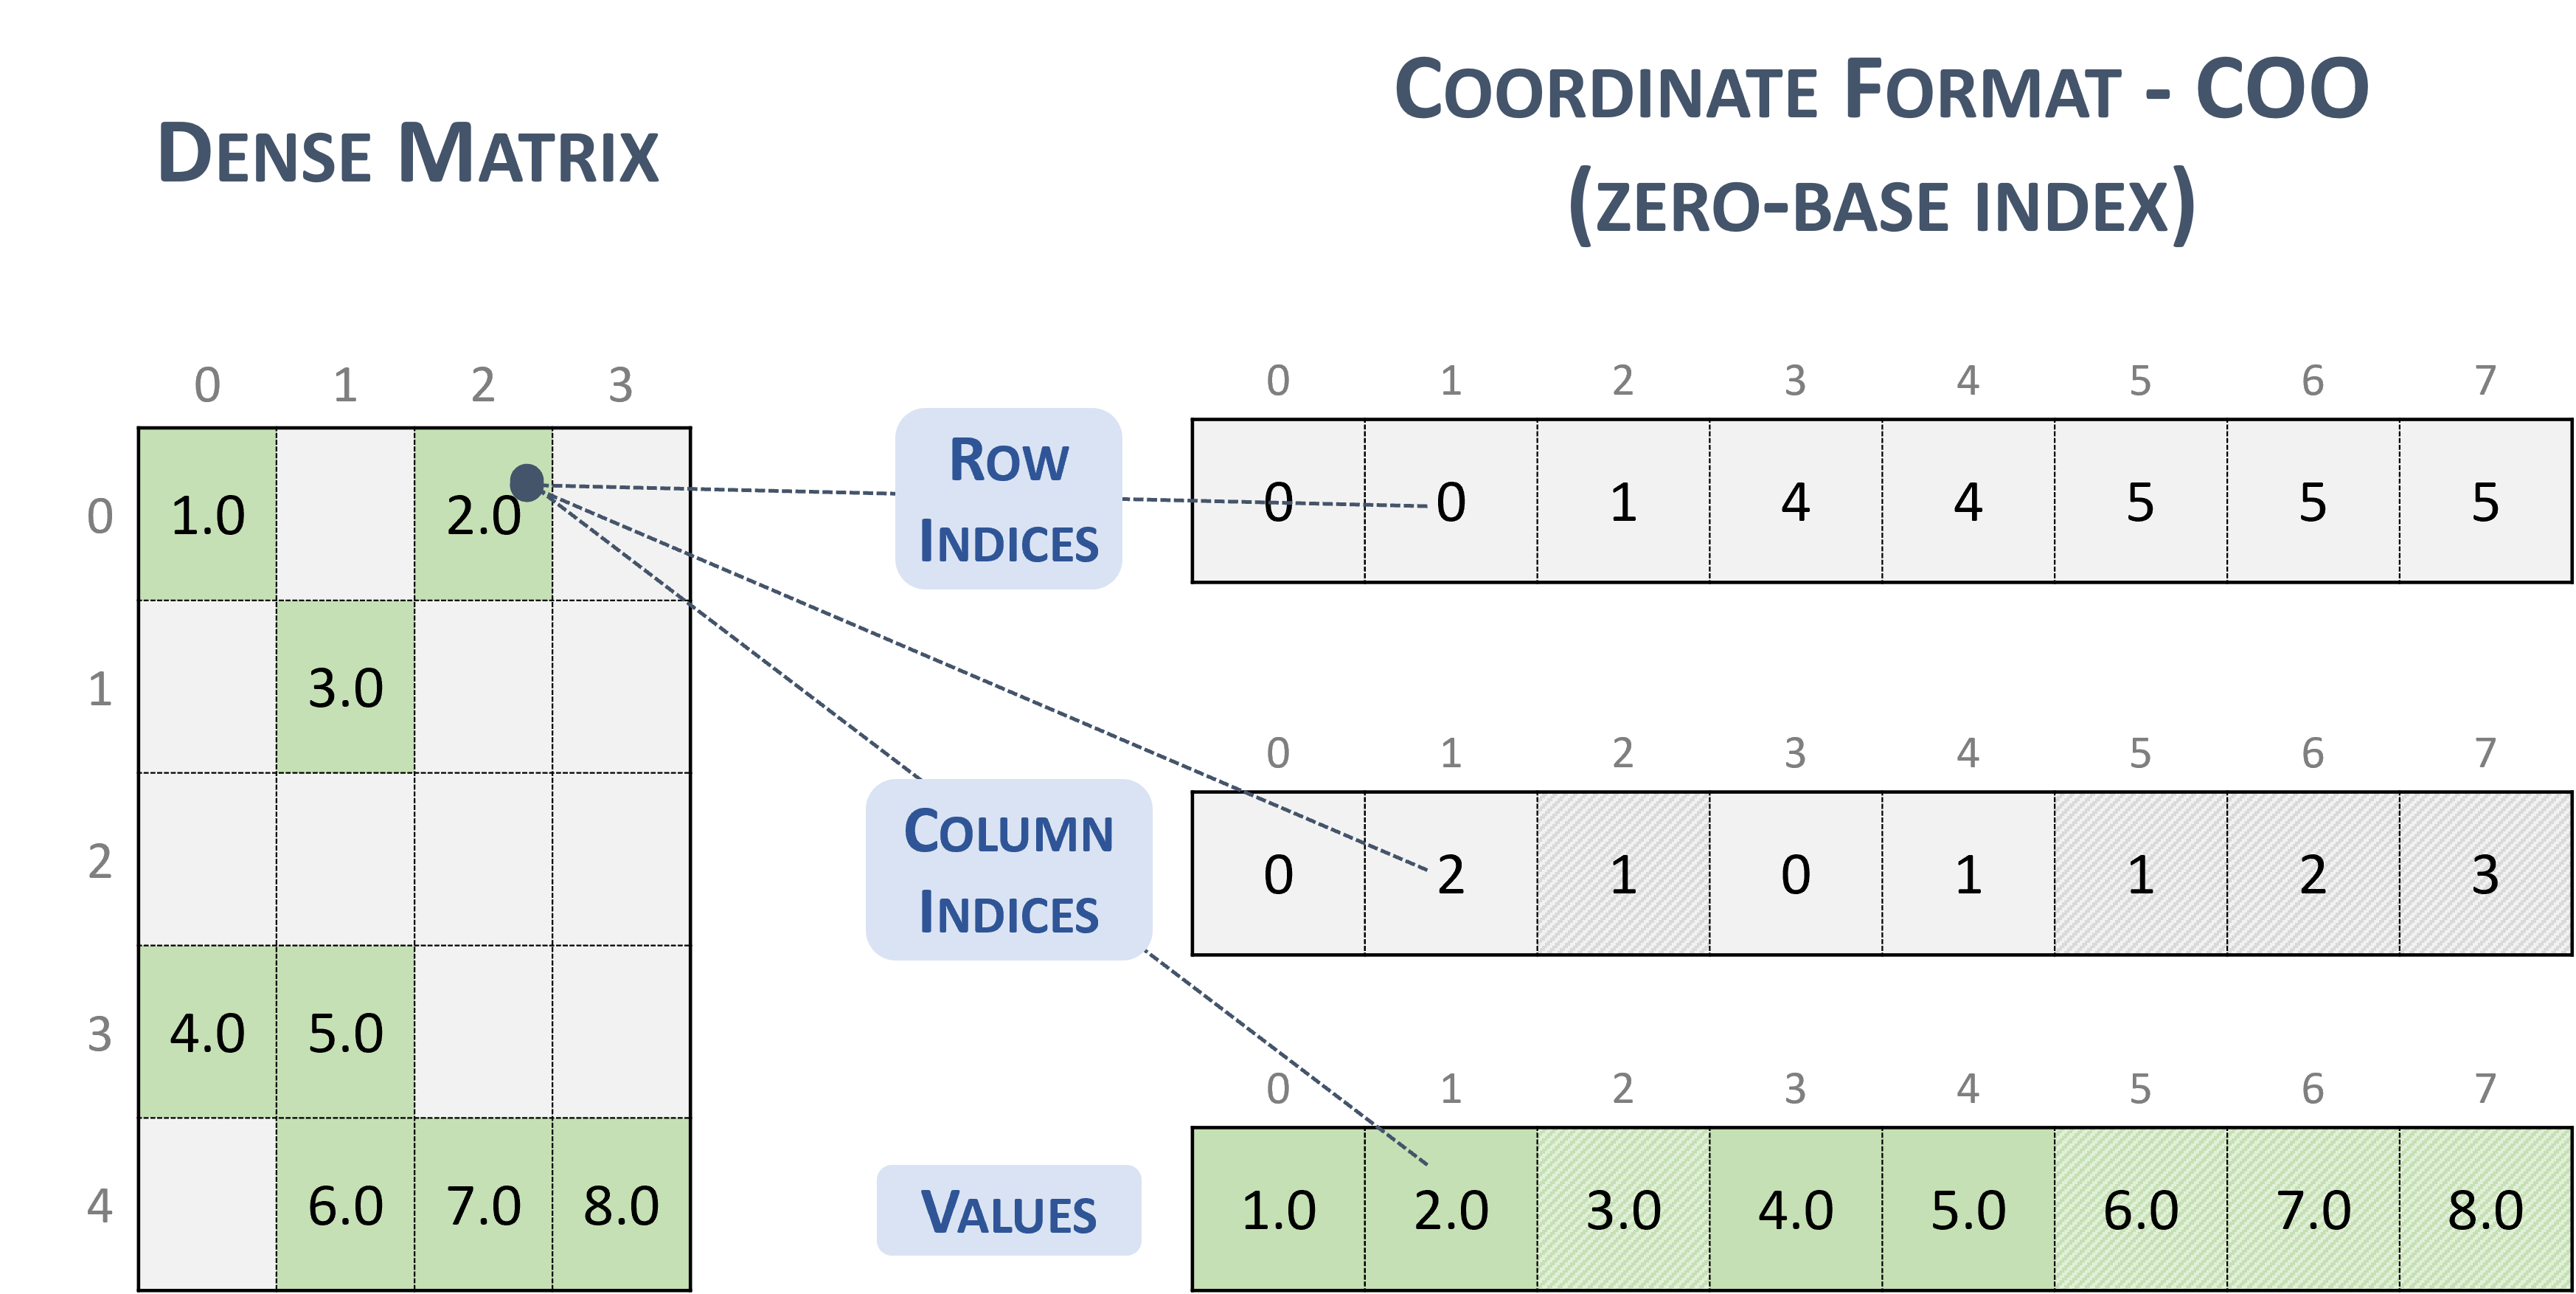
\includegraphics[width=\textwidth]{img/coo.png}
		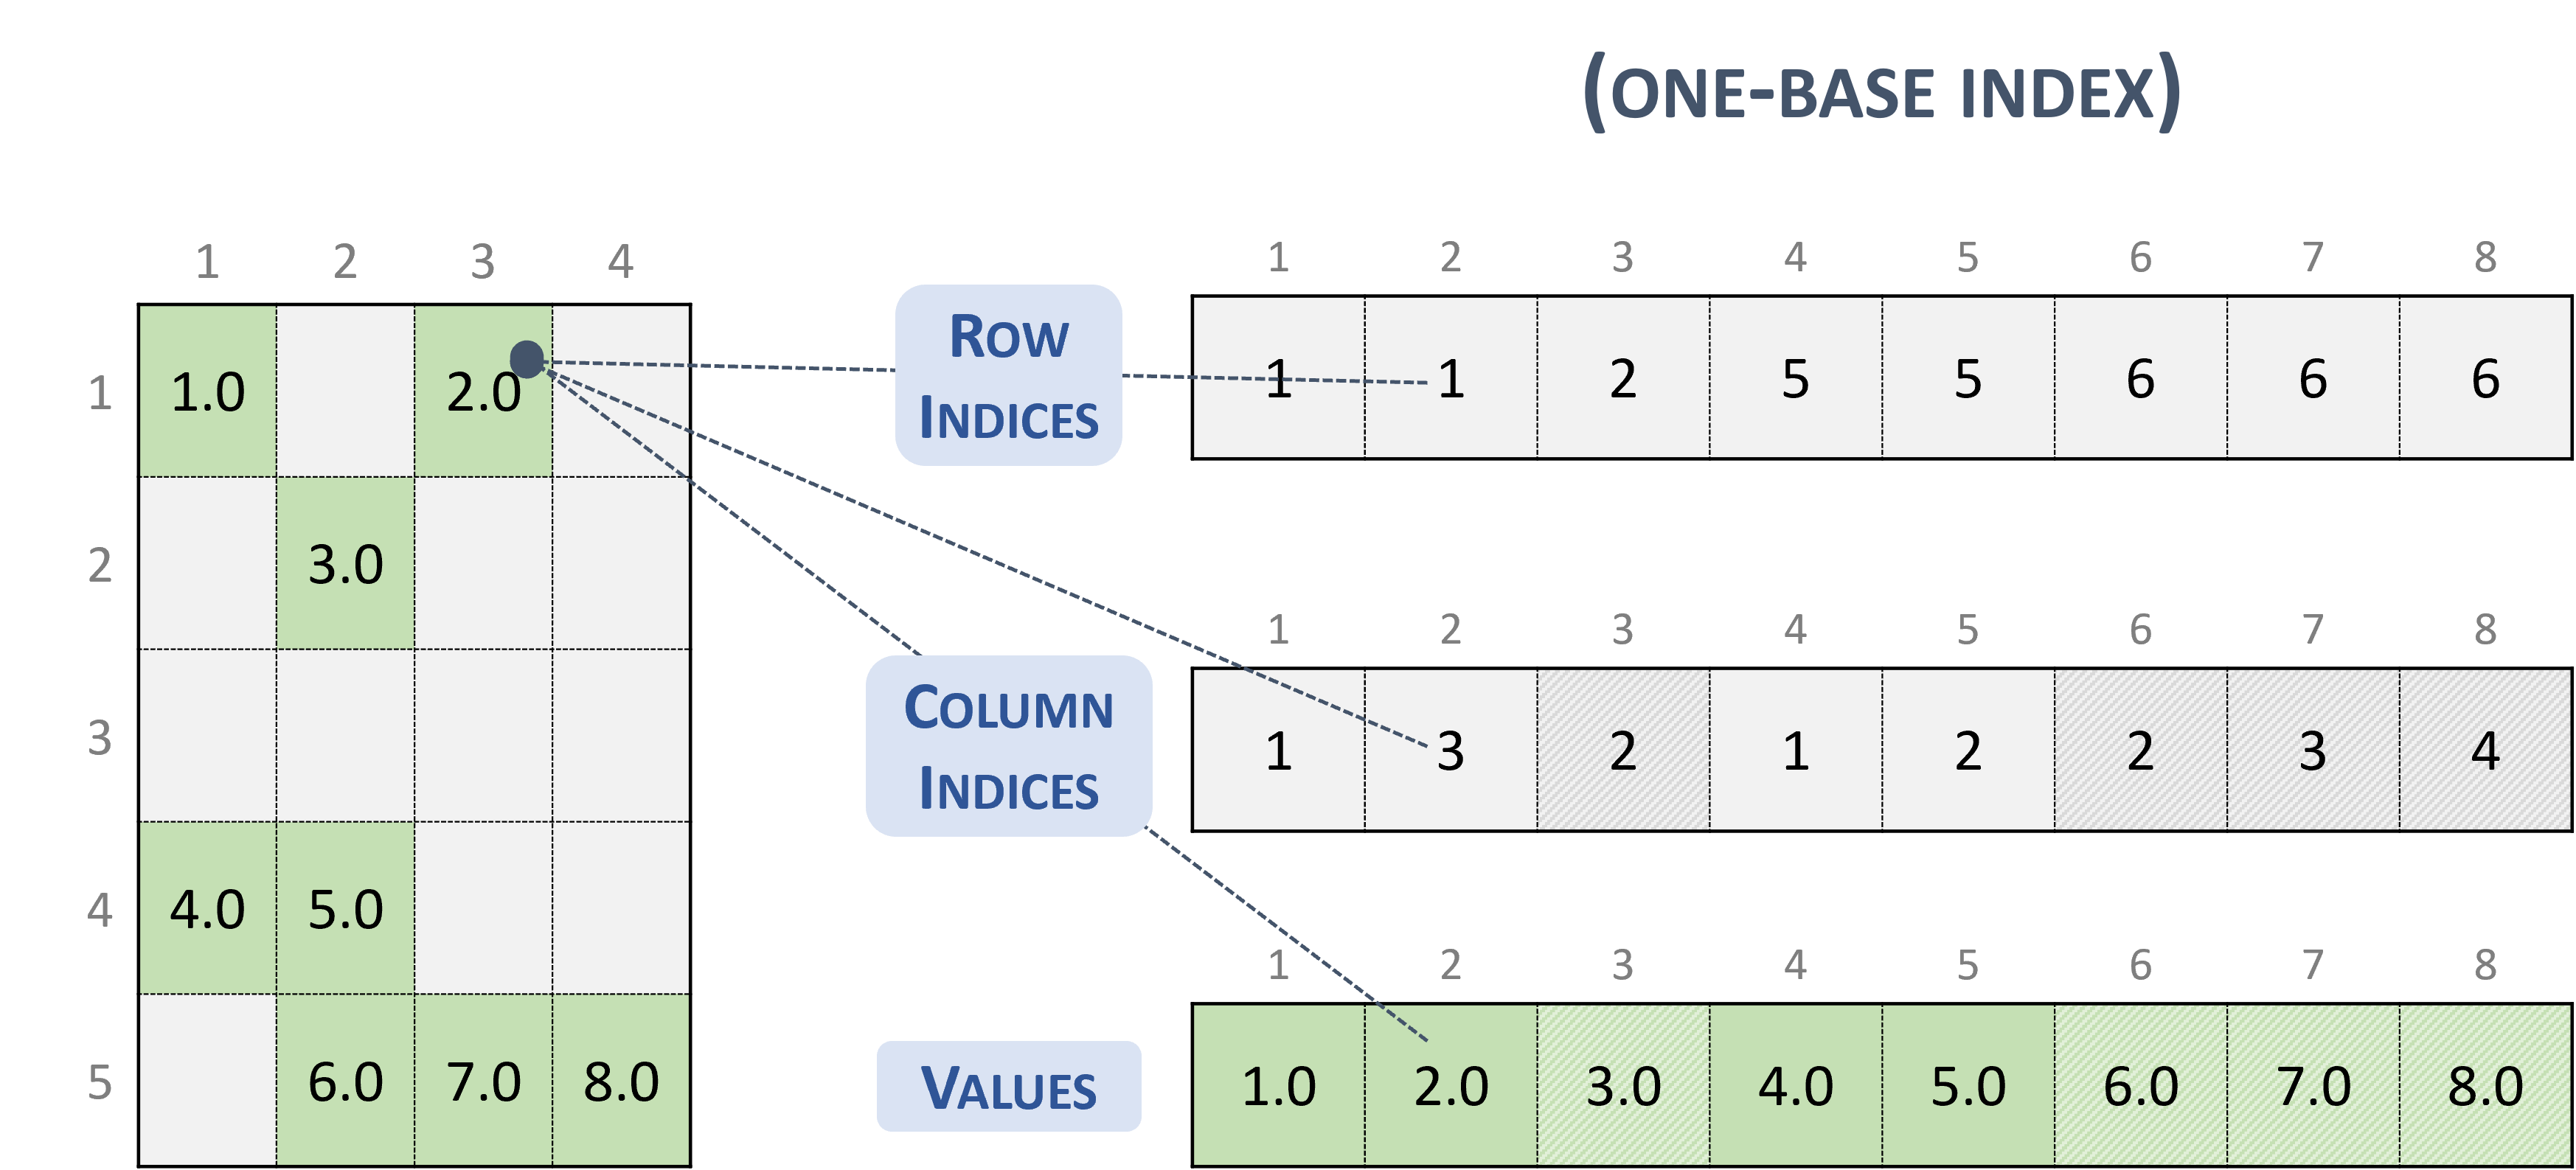
\includegraphics[width=\textwidth]{img/coo_one_base.png}
		\caption{Graphical representation of the coordinate format (COO) technique. From the figure we can see the representation of the \texttt{AA} array, called \emph{values}, the \texttt{JR}, called \emph{row indices}, and finally the \texttt{JC}, called \emph{column indices}. The algorithm is very simple. The figures are taken from the \href{https://docs.nvidia.com/nvpl/_static/sparse/storage_format/sparse_matrix.html}{NVIDIA Performance Libraries Sparse}, which is part of the \href{https://developer.nvidia.com/nvpl}{NVIDIA Performance Libraries}.}
	\end{figure}
	
	\item \definition{Coordinate Compressed Sparse Row format (CSR)}. If the elements of $A$ are listed by row, the array \texttt{JC} might be replaced by an array that points to the beginning of each row.
	\begin{itemize}
		\item \texttt{AA}: all the values of the non-zero elements of $A$, stored row by row from $1, \dots, n$.
		
		\item \texttt{JA}: contains the column indices.
		
		\item \texttt{IA}: contains the pointers to the beginning of each row in the arrays $A$ and \texttt{JA}. Thus \texttt{IA}$\left(i\right)$ contains the position in the arrays \texttt{AA} and \texttt{JA} where the $i$-th row starts. The length of \texttt{IA} is $n+1$, with $\texttt{IA}\left(n+1\right)$ containing the number $A\left(1\right) + \nnz\left(A\right)$. Remember that $n$ is the number of rows.
	\end{itemize}
	For \example{example}:
	\begin{equation*}
		A = \begin{bmatrix}
			1. & 0. & 0.& 2. & 0. \\
			3. & 4. & 0.& 5. & 0. \\
			6. & 0. & 7.& 8. & 9. \\
			0. & 0. & 10.& 11. & 0. \\
			0. & 0. & 0.& 0. & 12. 
		\end{bmatrix}
	\end{equation*}
	\begin{equation*}
		\begin{array}{rcl}
			\texttt{AA} &=& \left[
				1.\hspace{1em}
				2.\hspace{1em}
				3.\hspace{1em}
				\phantom{1}4.\hspace{1em}
				\phantom{1}5.\hspace{1em}
				\phantom{1}6.\hspace{1em}
				7.\hspace{1em}
				8.\hspace{1em}
				9.\hspace{1em}
				10.\hspace{1em}
				11.\hspace{1em}
				12.
			\right] \\ [.5em]
			\texttt{JA} &=& \left[
				1\phantom{.}\hspace{1em}
				4\phantom{.}\hspace{1em}
				1\phantom{.}\hspace{1em}
				\phantom{1}2\phantom{.}\hspace{1em}
				\phantom{1}4\phantom{.}\hspace{1em}
				\phantom{1}1\phantom{.}\hspace{1em}
				3\phantom{.}\hspace{1em}
				4\phantom{.}\hspace{1em}
				5\phantom{.}\hspace{1em}
				\phantom{1}3\phantom{.}\hspace{1em}
				\phantom{1}4\phantom{.}\hspace{1em}
				\phantom{1}5\phantom{.}
			\right] \\ [.5em]
			\texttt{IA} &=& \left[
				1\phantom{.}\hspace{1em}
				3\phantom{.}\hspace{1em}
				6\phantom{.}\hspace{1em}
				10\phantom{.}\hspace{1em}
				12\phantom{.}\hspace{1em}
				13\phantom{.}
			\right]
		\end{array}
	\end{equation*}
	To retrieve each position of the matrix, the algorithm is quite simple. Consider the \texttt{IA} arrays. 
	\begin{enumerate}
		\item We start at position one of the array, then the value 1:
		\begin{equation*}
			\begin{array}{rcl}
				\texttt{AA} &=& \left[
				1.\hspace{1em}
				2.\hspace{1em}
				3.\hspace{1em}
				\phantom{1}4.\hspace{1em}
				\phantom{1}5.\hspace{1em}
				\phantom{1}6.\hspace{1em}
				7.\hspace{1em}
				8.\hspace{1em}
				9.\hspace{1em}
				10.\hspace{1em}
				11.\hspace{1em}
				12.
				\right] \\ [.5em]
				\texttt{JA} &=& \left[
				1\phantom{.}\hspace{1em}
				4\phantom{.}\hspace{1em}
				1\phantom{.}\hspace{1em}
				\phantom{1}2\phantom{.}\hspace{1em}
				\phantom{1}4\phantom{.}\hspace{1em}
				\phantom{1}1\phantom{.}\hspace{1em}
				3\phantom{.}\hspace{1em}
				4\phantom{.}\hspace{1em}
				5\phantom{.}\hspace{1em}
				\phantom{1}3\phantom{.}\hspace{1em}
				\phantom{1}4\phantom{.}\hspace{1em}
				\phantom{1}5\phantom{.}
				\right] \\ [.5em]
				\texttt{IA} &=& \left[
				\circledtext{1}\phantom{.}\hspace{.4em}
				3\phantom{.}\hspace{1em}
				6\phantom{.}\hspace{1em}
				10\phantom{.}\hspace{1em}
				12\phantom{.}\hspace{1em}
				13\phantom{.}
				\right]
			\end{array}
		\end{equation*}
		
		
		\item We use the value one to see the first (index one) position of the array JA, and the value is 1:
		\begin{equation*}
			\begin{array}{rcl}
				\texttt{AA} &=& \left[
				1.\hspace{1em}
				2.\hspace{1em}
				3.\hspace{1em}
				\phantom{1}4.\hspace{1em}
				\phantom{1}5.\hspace{1em}
				\phantom{1}6.\hspace{1em}
				7.\hspace{1em}
				8.\hspace{1em}
				9.\hspace{1em}
				10.\hspace{1em}
				11.\hspace{1em}
				12.
				\right] \\ [.5em]
				\texttt{JA} &=& \left[
				\circledtext{1}\phantom{.}\hspace{.4em}
				4\phantom{.}\hspace{1em}
				1\phantom{.}\hspace{1em}
				\phantom{1}2\phantom{.}\hspace{1em}
				\phantom{1}4\phantom{.}\hspace{1em}
				\phantom{1}1\phantom{.}\hspace{1em}
				3\phantom{.}\hspace{1em}
				4\phantom{.}\hspace{1em}
				5\phantom{.}\hspace{1em}
				\phantom{1}3\phantom{.}\hspace{1em}
				\phantom{1}4\phantom{.}\hspace{1em}
				\phantom{1}5\phantom{.}
				\right] \\ [.5em]
				\texttt{IA} &=& \left[
				1\phantom{.}\hspace{1em}
				3\phantom{.}\hspace{1em}
				6\phantom{.}\hspace{1em}
				10\phantom{.}\hspace{1em}
				12\phantom{.}\hspace{1em}
				13\phantom{.}
				\right]
			\end{array}
		\end{equation*}
		
		\item But with the same index of \texttt{IA}, you also check the array \texttt{AA}, which has a value of 1:
		\begin{equation*}
			\begin{array}{rcl}
				\texttt{AA} &=& \left[
				\circledtext{1.}\hspace{.6em}
				2.\hspace{1em}
				3.\hspace{1em}
				\phantom{1}4.\hspace{1em}
				\phantom{1}5.\hspace{1em}
				\phantom{1}6.\hspace{1em}
				7.\hspace{1em}
				8.\hspace{1em}
				9.\hspace{1em}
				10.\hspace{1em}
				11.\hspace{1em}
				12.
				\right] \\ [.5em]
				\texttt{JA} &=& \left[
				1\phantom{.}\hspace{1em}
				4\phantom{.}\hspace{1em}
				1\phantom{.}\hspace{1em}
				\phantom{1}2\phantom{.}\hspace{1em}
				\phantom{1}4\phantom{.}\hspace{1em}
				\phantom{1}1\phantom{.}\hspace{1em}
				3\phantom{.}\hspace{1em}
				4\phantom{.}\hspace{1em}
				5\phantom{.}\hspace{1em}
				\phantom{1}3\phantom{.}\hspace{1em}
				\phantom{1}4\phantom{.}\hspace{1em}
				\phantom{1}5\phantom{.}
				\right] \\ [.5em]
				\texttt{IA} &=& \left[
				1\phantom{.}\hspace{1em}
				3\phantom{.}\hspace{1em}
				6\phantom{.}\hspace{1em}
				10\phantom{.}\hspace{1em}
				12\phantom{.}\hspace{1em}
				13\phantom{.}
				\right]
			\end{array}
		\end{equation*}
		
		\item Now we can check the next row of the matrix. So we check the array \texttt{IA} at position 2 and get the value 3. But be careful! From 1 (the previously calculated value) to 3 (the value just taken) there is the value 2 in between. So we can assume that the value 2 is also in the first row.
		\begin{equation*}
			\begin{array}{rcl}
				\texttt{AA} &=& \left[
				1.\hspace{1em}
				\circledtext{2.}\hspace{.6em}
				3.\hspace{1em}
				\phantom{1}4.\hspace{1em}
				\phantom{1}5.\hspace{1em}
				\phantom{1}6.\hspace{1em}
				7.\hspace{1em}
				8.\hspace{1em}
				9.\hspace{1em}
				10.\hspace{1em}
				11.\hspace{1em}
				12.
				\right] \\ [.5em]
				\texttt{JA} &=& \left[
				1\phantom{.}\hspace{1em}
				\circledtext{4}\phantom{.}\hspace{.4em}
				1\phantom{.}\hspace{1em}
				\phantom{1}2\phantom{.}\hspace{1em}
				\phantom{1}4\phantom{.}\hspace{1em}
				\phantom{1}1\phantom{.}\hspace{1em}
				3\phantom{.}\hspace{1em}
				4\phantom{.}\hspace{1em}
				5\phantom{.}\hspace{1em}
				\phantom{1}3\phantom{.}\hspace{1em}
				\phantom{1}4\phantom{.}\hspace{1em}
				\phantom{1}5\phantom{.}
				\right] \\ [.5em]
				\texttt{IA} &=& \left[
				1\phantom{.}\hspace{1.3em}
				3\phantom{.}\hspace{.7em}
				6\phantom{.}\hspace{1em}
				10\phantom{.}\hspace{1em}
				12\phantom{.}\hspace{1em}
				13\phantom{.}
				\right]
			\end{array}
		\end{equation*}
	\end{enumerate}
	\newpage
	\begin{figure}[!htp]
		\centering
		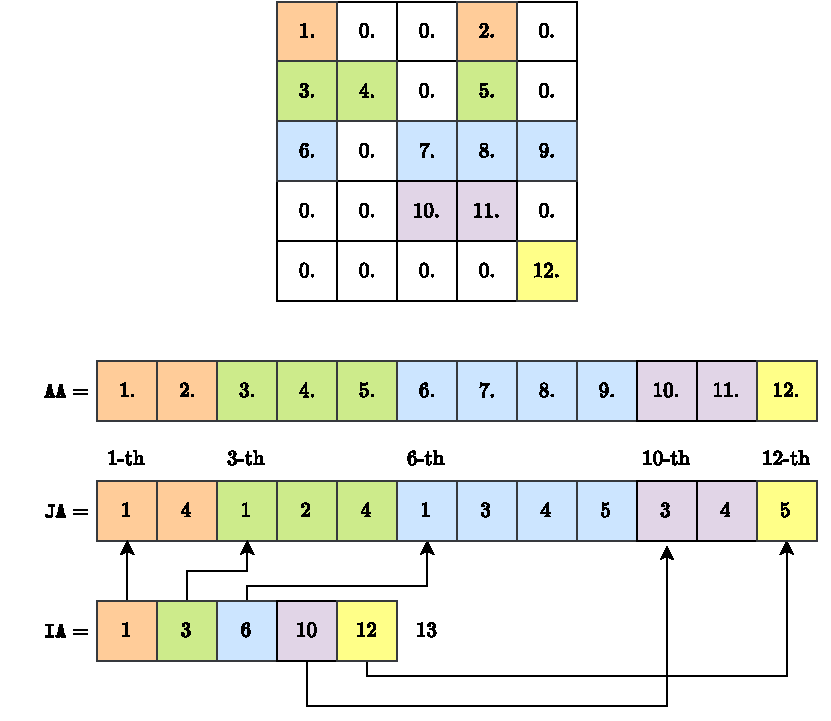
\includegraphics[width=\textwidth]{img/crs.pdf}
		\caption{View an illustration of the CRS technique using colors to improve readability.}
	\end{figure}
	\begin{figure}[!htp]
		\centering
		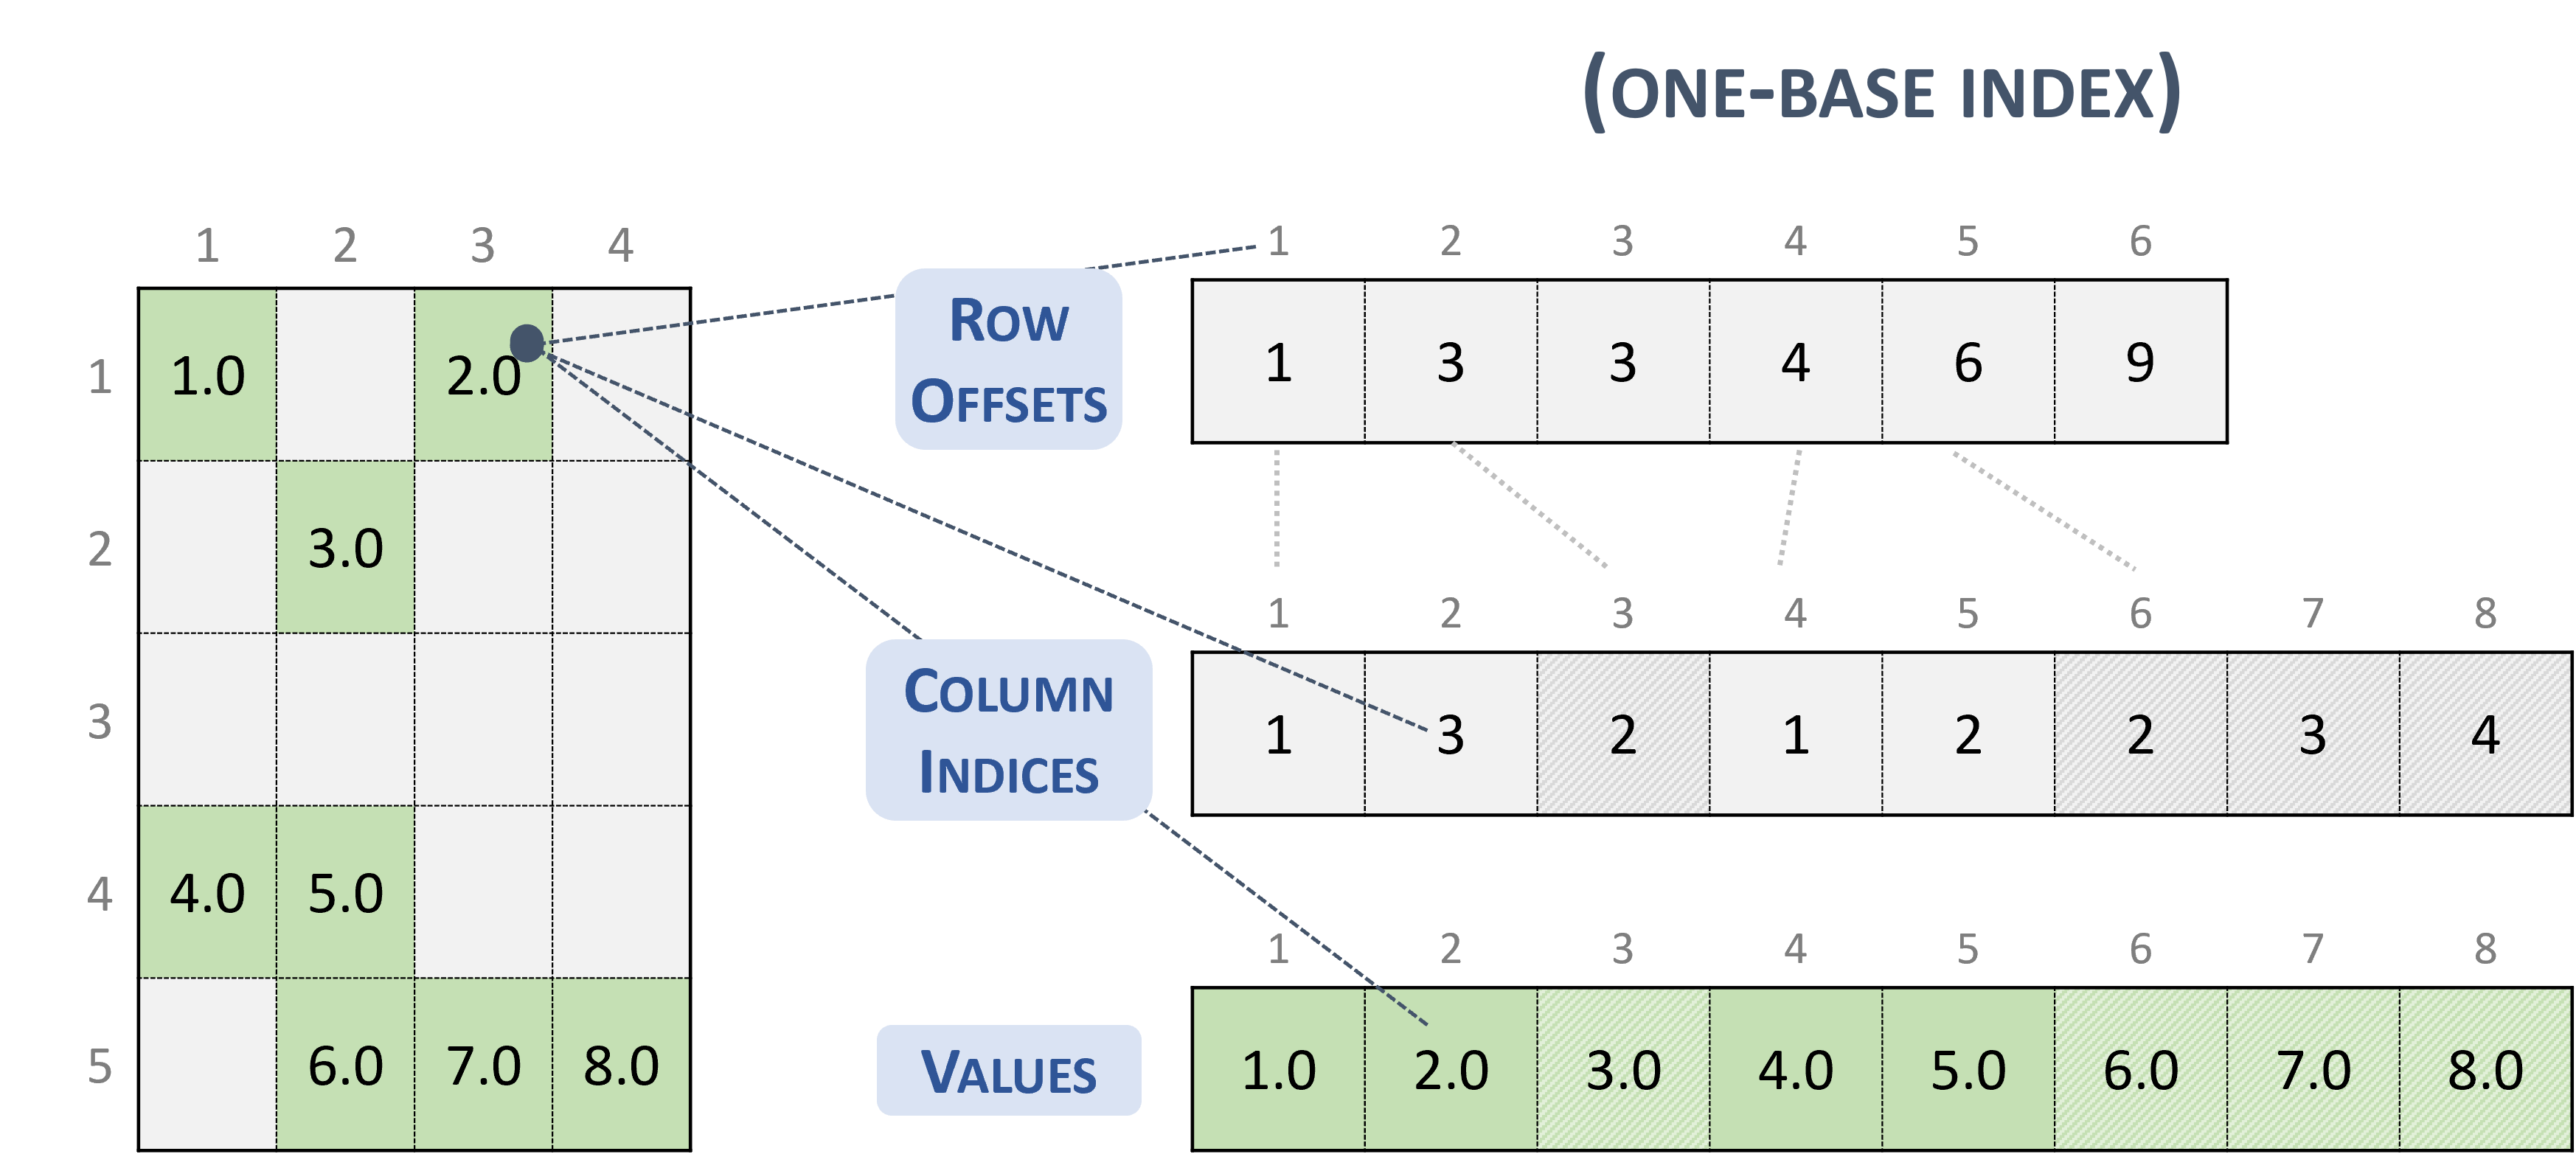
\includegraphics[width=.9\textwidth]{img/csr_one_base.png}
		\caption{Graphical representation of the coordinate compressed sparse row (CSR) technique. From the figure we can see the representation of the \texttt{AA} array, called \emph{values}, the \texttt{IA}, called \emph{row offset}, and finally the \texttt{JA}, called \emph{column indices}.
		It's interesting to see how the empty line case is handled. It copies the previous value of the array.
		The figures are taken from the \href{https://docs.nvidia.com/nvpl/_static/sparse/storage_format/sparse_matrix.html}{NVIDIA Performance Libraries Sparse}, which is part of the \href{https://developer.nvidia.com/nvpl}{NVIDIA Performance Libraries}.}
	\end{figure}
\end{itemize}

    %%%%%%%%%%%%%%%%%%%%%%%%%%%%%%%%%%%%%%%%%%%%%%%%%%%%%
    % Iterative methods for linear systems of equations %
    %%%%%%%%%%%%%%%%%%%%%%%%%%%%%%%%%%%%%%%%%%%%%%%%%%%%%
    \section{Iterative methods for linear systems of equations}

\subsection{Why not use the direct methods?}

Let us considering the following linear system of equations:
\begin{equation*}
    Ax = b
\end{equation*}
Where $A \in \mathbb{R}^{n \times n}$, $b \in \mathbb{R}^{n}$, $x \in \mathbb{R}^{n}$ and $\det\left(A\right) \ne 0$. In general, direct methods are \textbf{not very suitable whenever}:
\begin{itemize}
    \item \textbf{$n$ is large}. Typically, the average cost of direct methods scales as $n^{3}$, except in selected cases. As a trivial example, if peak performance is 1 PetaFLOPS ($10^{15}$ floating point operations per second), then
    \begin{equation*}
        n = 10^{7} \rightarrow \approx 10^{6} \text{ seconds} \approx 11 \text{ days}
    \end{equation*}
    \item \textbf{Matrix $A$ is sparse}. Direct methods suffer from the \emph{fill-in} phenomenon\footnote{The fill-in of a matrix are those entries that change from an initial zero to a non-zero value during the execution of an algorithm. To reduce the memory requirements and the number of arithmetic operations used during an algorithm, it is useful to minimize the fill-in.} (see later). Unfortunately, sparse matrices are very popular in many application problems and we cannot consider them.
\end{itemize}

\highspace
\begin{definitionbox}[: Sparse Matrix]
    Let $A \in \mathbb{R}^{n \times n}$ we say that $A$ is \definitionWithSpecificIndex{sparse}{Sparse Matrix} the number of non-zero elements (abbreviated as $\nnz\left(A\right)$) is approximately equal to the number of rows/columns $n$, i.e. $\nnz\left(A\right) \sim n$.
\end{definitionbox}

\highspace
\begin{flushleft}
    \textcolor{Green3}{\faIcon{question-circle} \textbf{What is an iterative method?}}
\end{flushleft}
It is clear that iterative methods are usually better than direct methods. An \definitionWithSpecificIndex{iterative method}{Iterative Method} is a \textbf{mathematical procedure that uses an initial value to generate a sequence of improving approximate solutions to a class of problems}, where the $i$-th approximation (called an \dquotes{\emph{iteration}}) is derived from the previous ones.

\highspace
More precisely, we introduce a sequence $\mathbf{x}^{\left(k\right)}$ of vectors determined by a recursive relation that identifies the method.
\begin{equation*}
    \mathbf{x}^{\left(0\right)} \rightarrow
    \mathbf{x}^{\left(1\right)} \rightarrow
    \cdots \rightarrow
    \mathbf{x}^{\left(k\right)} \rightarrow
    \mathbf{x}^{\left(k+1\right)} \rightarrow
    \cdots
\end{equation*}
To \dquotes{\emph{initialize}} the iterative process, it is necessary to provide a starting point (\emph{initial vector}, also called \emph{initial guess}) $\mathbf{x}^{\left(0\right)}$, e.g. based on physical/engineering applications.

\newpage

\noindent
After initialization, the core of the process should, sooner or later, produce a result. It is a very complex and long topic, but in general it refers to the process by which an iterative algorithm approaches a fixed point or a solution to a problem after several iterations. An \textbf{iterative method must satisfy the} \definitionWithSpecificIndex{convergence property}{Convergence property}:
\begin{equation}\label{eq: convergence property}
    \lim\limits_{k \rightarrow + \infty} \mathbf{x}^{\left(k\right)} = \mathbf{x}
\end{equation}
It is important to note that the \textbf{convergence \underline{does not depend} on the choice of the initial vector} $x^{\left(0\right)}$.

\highspace
From the property \ref{eq: convergence property}, it should be clear that \textbf{convergence is guaranteed only after an $\infty$ number of iterations}. From a practical point of view, we need to stop the iteration process after a finite number of iterations when we are \emph{sufficiently close} to the solution.

\highspace
In addition to the \emph{problem of convergence} and \dquotes{\emph{when should we stop our convergence method}}, we have to deal with the \emph{numerical error} inevitably introduced by our method.

\highspace
These topics will be explained and faced in the following pages.
    \subsection{Definition}

After a brief discussion of the difference between coherence and consistency terms, and why it is important to understand these concepts, here we present a deeper view of memory consistency. This is because consistency deals with the broader and more complex issue of how all memory operations (across all memory locations) are ordered and observed in a parallel system. It is also necessary to understand the high-level rules that govern the interactions between processors and memory in a multiprocessor environment.

\begin{definitionbox}[: Memory Consistency]
    \definition{Memory Consistency} models define \textbf{how memory operations} (loads and stores) \textbf{performed by different processors are \underline{ordered} and become visible to one another in a multiprocessor system}.
\end{definitionbox}

\highspace
\begin{flushleft}
    \textcolor{Green3}{\faIcon{question-circle} \textbf{Why the order decided by the memory consistency model is important}}
\end{flushleft}
One main reason:
\begin{itemize}
    \item \textbf{Performance}. In multiprocessor systems, memory operations can be reordered to optimize performance. Unfortunately, this \textbf{reordering can result in behavior that seems counterintuitive or unusual from the perspective of a programmer} who expects sequential execution. However, it allows optimizations such as overlapping memory accesses with computations and reducing memory access latency.
\end{itemize}
Most application programmers don't have to deal directly with the effects of memory reordering, because higher-level constructs and synchronization mechanisms handle them. However, understanding memory consistency is critical to writing correct and efficient parallel programs. Developers of system software, such as operating systems and compilers, must deal with these issues to ensure that their low-level code conforms to the hardware's memory consistency model and maintains the correct order of memory operations.

\newpage

\begin{flushleft}
    \hqlabel{flushleft: Memory Operation Ordering}{\textcolor{Green3}{\faIcon{sort-amount-up-alt} \textbf{Memory Operation Ordering}}}
\end{flushleft}
A program defines a sequence of loads and saves. There are \textbf{four types of memory operation sequences}:
\begin{enumerate}
    \item \important{$W_{X} \rightarrow R_{Y}$}: \textbf{Write to $X$ must commit before a subsequent read from $Y$}.

    This means that if a write to memory location $X$ occurs before a read from another memory location $Y$ in the program order, the write must be complete and visible before the read.


    \item \important{$R_{X} \rightarrow R_{Y}$}: \textbf{Read from $X$ must commit before a subsequent read from $Y$}.
   
    This order ensures that if a read from $X$ occurs before a read from $Y$ in the program, the first read must be completed before the second read occurs.


    \item \important{$R_{X} \rightarrow W_{Y}$}: \textbf{Read from $X$ must commit before a subsequent write to $Y$}.
   
    This means that if a read from $X$ occurs before a write to $Y$ in the program order, the read must be completed before the write is performed.


    \item \important{$W_{X} \rightarrow W_{Y}$}: \textbf{Write to $X$ must commit before a subsequent write to $Y$}.
   
    This ordering ensures that if a write to $X$ happens before a write to $Y$ in the program, the first write must be completed before the second write is performed.
\end{enumerate}
The word \dquotes{subsequent} means that each left operation must be completed and its result visible before the right operation can occur.

    \subsubsection{Jacobi method}

Let the problem of solve $Ax = b$, where $A$ is a square matrix, $x$ is the vector of unknowns, and $b$ is the result vector.

\highspace
We start from the $i$-th line of the linear system:
\begin{equation*}
    \displaystyle\sum_{j = 1}^{n} a_{ij}x_{j} = b_{i} \: \rightarrow \: a_{i1}x_{1} + a_{i2}x_{2} + \cdots + a_{in}x_{n} = b_{i}
\end{equation*}
Formally the solution $x_{i}$ for each $i$ si given by:
\begin{equation}
    x_{i} = \dfrac{b_{i}-\displaystyle\sum_{j \ne i} a_{ij}x_{j}}{a_{ii}}
\end{equation}
Obviously the previous identity cannot be used in practice because we do not know $x_{j}$, for $j \ne i$. And here is the \textbf{magic idea} of Jacobi: we could think of introducing an iterative method (Jacobi) that \textbf{updates} $x_{i}^{\left(k+1\right)}$ \textbf{step} $k+1$ \textbf{using the other} $x_{j}^{\left(k\right)}$ \textbf{obtained in the previous step} $k$.
\begin{equation}\label{eq: jacobi x calcolus}
    x_{i} = \dfrac{b_{i}-\displaystyle\sum_{j \ne i} a_{ij}x_{j}}{a_{ii}} \: \xRightarrow{\text{as }x_{j}\text{ is not well known}} \: x_{i}^{\left(k+1\right)} = \dfrac{b_{i}-\displaystyle\sum_{j \ne i} a_{ij}x_{j}^{\left(k\right)}}{a_{ii}}
\end{equation}
Where $\forall i = 1, \dots, n$.

\highspace
\begin{flushleft}
    \textcolor{Green3}{\faIcon{tools} \textbf{Algorithm}}
\end{flushleft}
\begin{enumerate}
    \item \textbf{Start with an initial guess} $\mathbf{x}^{\left(0\right)}$, also zero.
    \item \textbf{Update each component} $\mathbf{x}_{i}^{\left(k+1\right)}$ using the equation \ref{eq: jacobi x calcolus}.
    \item \textbf{Repeat until the changes are less than a specified tolerance} or we haven't found the exact solution (in practice very difficult, almost impossible).
\end{enumerate}

\highspace
\begin{flushleft}
    \textcolor{Red2}{\faIcon{dollar-sign} \textbf{How much does it cost?}}
    \label{general-ref: cost jacobi method}
\end{flushleft}
It depends on the matrix used:
\begin{itemize}
    \item \textbf{Dense matrix} (bad choice). Each iteration costs $\approx n^{2}$ operations, so the Jacobi method is competitive if the number of iteration is less than $n$.
    \item \textbf{Sparse matrix} (good choice). Each iteration costs only $\approx n$ operations.
\end{itemize}

\highspace
\begin{flushleft}
    \textcolor{Green3}{\faIcon{network-wired} \textbf{Can it be parallelized?}}
\end{flushleft}
The parallelization of the Jacobi method is actually \textbf{one of its main advantages} on modern computers. Each update of $x_{i}$ depends only on the previous values of the other $x_{j}$, not on the current iteration values. This independence makes it easy to distribute the work across multiple processors.

    \subsubsection{Gauss-Seidel method}

Given the Jacobi method, the Gauss Seidel method is similar, but with one clever difference: it uses the latest available values during iterations.
\begin{equation}\label{eq: gauss seidel x calcolus}
    x_{i}^{\left(k+1\right)} = \dfrac{b_{i} - \displaystyle\sum_{j < i} a_{ij}x_{j}^{\left(k+1\right)} - \displaystyle\sum_{j > i}a_{ij}x_{j}^{\left(k\right)}}{a_{ii}}
\end{equation}
At iteration $\left(k+1\right)$, let's consider the computation of $x_{i}^{\left(k+1\right)}$. We observe that for $j < i$ (with $i \ge 2$), $x_{j}^{\left(k+1\right)}$ is known (we have already calculated it). We can therefore think of using the quantities at step $\left(k+1\right)$ if $j<i$ and, as in the Jacobi method, those at the previous step $k$ if $j > i$.

\highspace
\begin{flushleft}
    \textcolor{Green3}{\faIcon{tools} \textbf{Algorithm}}
\end{flushleft}
\begin{enumerate}
    \item \textbf{Start with an initial guess} $\mathbf{x}^{\left(0\right)}$, also zero.
    \item \textbf{Iteration}. For each row $i$ from $1$ to $n$ calculate the value of the equation \ref{eq: gauss seidel x calcolus}.
    \item \textbf{Repeat until the changes are less than a specified tolerance}.
\end{enumerate}

\highspace
\begin{flushleft}
    \textcolor{Red2}{\faIcon{dollar-sign} \textbf{How much does it cost?}}
\end{flushleft}
The cost is comparable to the Jacobi method explained on page \pageref{general-ref: cost jacobi method}.

\highspace
\begin{flushleft}
    \textcolor{Green3}{\faIcon{network-wired} \textbf{Can it be parallelized?}}
\end{flushleft}
Unlike the Jacobi method, the Gauss-Seidel method relies on the most recent updates within the same iteration. This sequential dependency \textbf{makes it more difficult to parallelize, as each update depends on the previous ones}.

\highspace
While it's harder to parallelize due to its inherent sequential nature, we can still achieve some degree of parallelism with clever strategies such as red-black ordering. This makes the Gauss-Seidel method less straightforward to parallelize than Jacobi, but not impossible.

    \subsubsection{Convergence of Jacobi and Gauss-Seidel methods}

Let be a general matrix $A$, and :
\begin{itemize}
    \item $D$ the \textbf{diagonal part} of $A$
    \item $-E$ \textbf{lower triangular part} of $A$
    \item $-F$ \textbf{upper triangular part} of $A$
\end{itemize}
\begin{equation*}
    A = \begin{bmatrix}
        & & & & \\
        & \ddots &   & -F     & \\
        &        & D &        & \\
        & -E     &   & \ddots & \\
        & & & &
    \end{bmatrix}
\end{equation*}
The previous Jacobi and Gauss-Seidel methods can be rewritten as:
\begin{itemize}
    \item Jacobi:
    \begin{itemize}
        \item Method:
        \begin{equation*}
            D\mathbf{x}^{\left(k+1\right)} = \left(E+F\right)\mathbf{x}^{\left(k\right)} + \mathbf{b}
        \end{equation*}
        \item Iteration matrix:
        \begin{equation*}
            B_{J} = D^{-1}\left(E+F\right) = D^{-1}\left(D-A\right) = I-D^{-1}A
        \end{equation*}
    \end{itemize}

    \item Gauss-Seidel
    \begin{itemize}
        \item Method:
        \begin{equation*}
            \left(D-E\right)\mathbf{x}^{\left(k+1\right)} = F\mathbf{x}^{k} + \mathbf{b}
        \end{equation*}
        \item Iteration matrix:
        \begin{equation*}
            B_{GS} = \left(D-E\right)^{-1}F
        \end{equation*}
    \end{itemize}
\end{itemize}
We present a theorem which gives us the \textbf{sufficient condition for convergence} of the Jacobi and Gauss-Seidel methods.

\begin{theorem}[\textbf{sufficient condition for convergence of Jacobi and Gauss-Seidel}]
    The following conditions are sufficient for convergence:
    \begin{itemize}
        \item If a matrix $A$ is \textbf{strictly diagonally dominant by \underline{rows}}:
        \begin{equation*}
            \left|a_{ii}\right| > \displaystyle\sum_{j \ne i} \left|a_{ij}\right| \hspace{2em} i = 1, \dots, n
        \end{equation*}
        Then Jacobi and Gauss-Seidel converge.

        \item If a matrix $A$ is \textbf{strictly diagonally dominant by \underline{columns}}:
        \begin{equation*}
            \left|a_{ii}\right| > \displaystyle\sum_{j \ne i} \left|a_{ji}\right| \hspace{2em} i = 1, \dots, n
        \end{equation*}
        Then Jacobi and Gauss-Seidel converge.

        \item If a matrix $A$ is SPD (symmetric positive and definite), then the Gauss-Seidel method is convergent.
        
        \item If a matrix $A$ is tridiagonal\footnote{A matrix is \definitionWithSpecificIndex{tridiagonal}{Tridiagonal matrix} when it has non-zero elements only on the main diagonal, the diagonal above the main diagonal, and the diagonal below the main diagonal.
        \begin{equation*}
            A = \begin{bmatrix}
                a_{1,1} & a_{1,2} & 0       & 0  \\
                a_{2,1} & a_{2,2} & a_{2,3} & 0  \\
                0 & a_{3,2} & a_{3,3} & a_{3,4} \\
                0 & 0 & a_{4,3} & a_{4,4} \\
            \end{bmatrix}
        \end{equation*}
        }, then the square spectral value of the Jacobi iteration matrix is equal to the spectral value of the Gauss-Seidel iteration matrix.
        \begin{equation*}
            \rho^{2}\left(B_{J}\right) = \rho\left(B_{GS}\right)
        \end{equation*}
    \end{itemize}
\end{theorem}

    \subsubsection{The stationary Richardson method}

The stationary Richardson method is a way of refining a guess for solving the general problem $Ax = b$. We \textbf{start with an initial guess for the solution}, then we \textbf{keep adjusting that guess based on how far it is from the actual answer}. The \textbf{adjustments depend on a parameter we choose}, which can speed up or slow down how quickly we get to the right answer. We \textbf{keep doing this until our guess is close enough to the actual solution}.

\highspace
Mathematically, given $\mathbf{x}^{\left(0\right)} \in \mathbb{R}^{n}$, $\alpha \in \mathbb{R}$, the stationary Richardson method is based on the following recursive update:
\begin{equation}\label{eq: stationary richardson x calcolus}
    \mathbf{x}^{\left(k+1\right)} = \mathbf{x}^{\left(k\right)} + \alpha \cdot \underbrace{\left(\mathbf{b} - A\mathbf{x}^{\left(k\right)}\right)}_{\text{residual }\mathbf{r}^{\left(k\right)}}
\end{equation}
The idea is to update the numerical solution by adding a quantity proportional to the residual. Indeed, it is expected that if the residual is \emph{large} (\emph{small}), the solution at step $k$ should be corrected \emph{much} (\emph{little}). Where $\alpha$ is a weighted version of the residual.
\begin{itemize}
    \item Iteration matrix $B_{\alpha}$:
    \begin{equation*}
        B_{\alpha} = I - \alpha A
    \end{equation*}
    \item $\mathbf{f}$:
    \begin{equation*}
        \mathbf{f} = \alpha \mathbf{b}
    \end{equation*}
\end{itemize}
We now ask ourselves \textbf{which value of the parameter} $\alpha$, among those that \textbf{guarantee convergence}, \textbf{maximizes the speed of convergence}. We introduce the following $A$-induced norm where A is SPD:
\begin{equation*}
    {\left|\left|\mathbf{z}\right|\right|}_{A} = \sqrt{
        \displaystyle\sum_{i,j = 1}^{n} a_{ij}z_{i}z_{j}
    }
    \iff
    {\left|\left|\mathbf{z}\right|\right|}_{A} = \sqrt{\left(A\mathbf{z}, \mathbf{z}\right)} = \sqrt{\mathbf{z}^{T} A \mathbf{z}}
\end{equation*}
We look for $0 < \alpha_{\text{opt}} < \dfrac{2}{\lambda_{\max\left(A\right)}}$ such that $\rho\left(B_{\alpha}\right)$ is minimum. That is:
\begin{equation*}
    \alpha_{\text{opt}} = \underset{0 < \alpha < \frac{2}{\lambda_{\max\left(A\right)}}}{\mathrm{argmin}} \left\{\underset{i}{\max} \left|1 - \alpha\lambda_{i}\left(A\right)\right|\right\}
\end{equation*}
To understand which $\alpha$ to choose, we plot the problem. On the \emph{x-axis} are the values of $\alpha$ and on the \emph{y-axis} is the spectral radius equal to $\left|1-\alpha\lambda_{i}\left(A\right)\right|$, with $i = 1, \dots, n$.

\highspace
In the figure \ref{fig: alpha stationary Richardson method} we can see that the upper bound of the spectral radius is equal to 1 (no convergence). Each line represents the possible value of the spectral radius for different values of $\alpha$. In \textbf{green} we see the \textbf{spectral radius equal to} $\rho\left(B_{\alpha}\right)$; it is important because its intersection with the upper bound of $\rho$ represents the right bound of the interval where the \textbf{values of $\alpha$ guarantee convergence}. It can also be seen by the \textbf{red arrow}. The \textbf{lowest point of the curve is where the spectral radius is minimized, indicating the best $\alpha$ for convergence}.

\highspace
In other words, the optimal value is given by the intersection between the curves:
\begin{equation*}
    \left|1 - \alpha \lambda_{1}\left(A\right)\right|
    \cap
    \left|1 - \alpha \lambda_{n}\left(A\right)\right|
\end{equation*}
That gives us the perfect formula:
\begin{equation}
    \alpha_{\text{opt}} = \dfrac{2}{\lambda_{\min}\left(A\right) + \lambda_{\max}\left(A\right)}
\end{equation}
\begin{figure}[!htp]
    \centering
    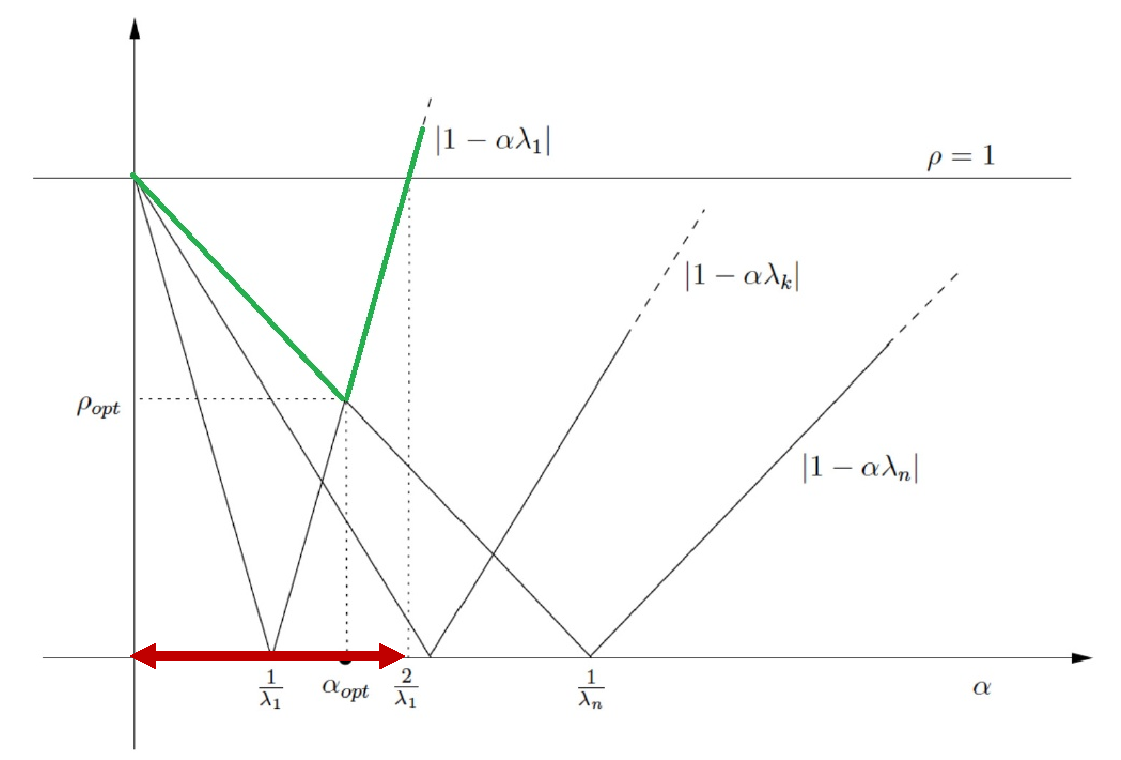
\includegraphics[width=\textwidth]{img/richardson-alpha-opt-1.pdf}
    \caption{Graphical representation of the optimal alpha to choose in the stationary Richardson method.}
    \label{fig: alpha stationary Richardson method}
\end{figure}

\noindent
If A is SPD, the eigenvalues of $A$ (real and positive) are:
\begin{equation*}
    \lambda_{\max}\left(A\right) = \lambda_{1}\left(A\right) \ge \lambda_{2}\left(A\right) \ge \cdots \ge \lambda_{n}\left(A\right) = \lambda_{\min}\left(A\right) > 0
\end{equation*}
\begin{theorem}
    Let A be a symmetric and positive definite matrix. The \textbf{stationary Richardson method is convergent if and only if}:
    \begin{equation}
        0 < \alpha < \dfrac{2}{\lambda_{\max}\left(A\right)}
    \end{equation}
\end{theorem}

\noindent
Since there is a strong correlation between the optimal $\alpha$ and the optimal spectral radius, we can obtain
\begin{equation*}
    \begin{array}{rcl}
        \rho_{\text{opt}} &=& \rho\left(B_{\alpha_{\text{opt}}}\right) \\ [.3em]
        &=& -1+\alpha_{\text{opt}}\lambda_{\max}\left(A\right) \\ [.3em]
        &=& 1-\alpha_{\text{opt}}\lambda_{\min}\left(A\right) \\ [.3em]
        &=& \dfrac{
            \lambda_{\max}\left(A\right) - \lambda_{\min}\left(A\right)
        }{
            \lambda_{\max}\left(A\right) + \lambda_{\min}\left(A\right)
        }
    \end{array}
\end{equation*}
Finally, since $A$ is SPD, we have the Euclidean norm equal to the maximum eigenvalue of A: ${\left|\left|A\right|\right|}_{2} = \lambda_{\max}\left(A\right)$. Moreover, $\lambda_{i}\left(A^{-1}\right) = \frac{1}{\lambda_{i}\left(A\right)}$, $i = 1, \dots, n$:
\begin{equation}
    \rho_{\text{opt}} = \dfrac{
        K\left(A\right)-1
    }{
        K\left(A\right)+1
    }
\end{equation}

\begin{flushleft}
    \textcolor{Green3}{\faIcon{tools} \textbf{Algorithm}}
\end{flushleft}
\begin{enumerate}
    \item \textbf{Start with an initial guess} $x^{\left(0\right)}$ and \textbf{select a parameter} $\alpha$.
    \item \textbf{Iteration}. For each $k$ calculate the value of the equation \ref{eq: stationary richardson x calcolus}.
    \item \textbf{Repeat until the changes are less than a specified tolerance}.
\end{enumerate}

\highspace
\begin{flushleft}
    \textcolor{Red2}{\faIcon{dollar-sign} \textbf{How much does it cost?}}
\end{flushleft}
The cost of each iteration depends by type of matrix:
\begin{itemize}
    \item \textbf{Dense matrix}: the cost of each iteration is about $n^{2}$ \textbf{operations}, where $n$ is the number of unknowns in the linear system.
    \item \textbf{Sparse matrix}: the cost of each iteration is only about $n$ \textbf{operations}.
\end{itemize}

\highspace
\begin{flushleft}
    \textcolor{Green3}{\faIcon{network-wired} \textbf{Can it be parallelized?}}
\end{flushleft}
The stationary Richardson method is not as easily parallelizable as the Jacobi method. Richardson uses the entire solution vector from the previous iteration in each step. This dependency makes it \textbf{more difficult to parallelize}.
    \subsection{Stopping Criteria}

A practical test is needed to determine when to stop the iteration. The \textbf{main idea} is that we stop iterations when:
\begin{equation*}
    \dfrac{\left|\left|\mathbf{x} - \mathbf{x^{\left(k\right)}}\right|\right|}{\left|\left|\mathbf{x}^{\left(k\right)}\right|\right|} \le \varepsilon
\end{equation*}
Where $\varepsilon$ is a \textbf{user defined tolerance}. Meanwhile, the error (left side of the equation) is unknown! There are two criteria we can use to replace it:
\begin{itemize}
    \item \definition{Residual-based stopping criteria}. It looks at the \emph{residual}, which is the difference between the current solution and the one obtained by reapplying the method's equation:
    \begin{equation*}
        r^{\left(k\right)} = b - Ax^{\left(k\right)}
    \end{equation*}
    This residual gets smaller as the solution gets closer to the exact answer. When it's small enough, the iteration stops. This approach works because the residual essentially tracks the behaviour of the error. When the residual is small, the error is usually small.
    
    From a mathematical point of view:
    \begin{equation*}
        \dfrac{\left|\left|\mathbf{x} - \mathbf{x^{\left(k\right)}}\right|\right|}{\left|\left|\mathbf{x}^{\left(k\right)}\right|\right|} \le K\left(A\right) \dfrac{\left|\left|\mathbf{r}^{\left(k\right)}\right|\right|}{\left|\left|\mathbf{b}\right|\right|} \Longrightarrow \dfrac{\left|\left|\mathbf{r}^{\left(k\right)}\right|\right|}{\left|\left|\mathbf{b}\right|\right|} \le \varepsilon
    \end{equation*}
    Where $K\left(A\right)$ is the \definitionWithSpecificIndex{condition number}{Condition Number} of $A$. It is a measure of \textbf{how sensitive the solution of a system of linear equations is to errors in the data or errors in the solution process}.
    \begin{itemize}
        \item A \textbf{low condition number} (close to 1) means that the matrix is well conditioned, and \textbf{small errors in the data will cause only small errors in the solution}.

        \item A \textbf{high condition number} indicates that the matrix is poorly conditioned, and even \textbf{small errors in the data can lead to large errors in the solution}.
    \end{itemize}
    To reduce the condition number and the error, we need to use a preconditioner on the main matrix $A$. So instead of solving the general problem $Ax = b$ directly, we choose a preconditioner $P$ and solve $P^{-1}Ax = P^{-1}b$:
    \begin{equation*}
        \dfrac{\left|\left|\mathbf{x} - \mathbf{x^{\left(k\right)}}\right|\right|}{\left|\left|\mathbf{x}^{\left(k\right)}\right|\right|} \le K\left(P^{-1} A\right) \dfrac{\left|\left|\mathbf{z}^{\left(k\right)}\right|\right|}{\left|\left|\mathbf{b}\right|\right|} \Longrightarrow
        \dfrac{\left|\left|\mathbf{z}^{\left(k\right)}\right|\right|}{\left|\left|\mathbf{b}\right|\right|} \le \varepsilon \hspace{2em} \mathbf{z}^{\left(k\right)} = P^{-1}\mathbf{r^{\left(k\right)}}
    \end{equation*}

    \item \definition{Distance between consecutive iterates criteria}. It looks at \textbf{how much the current iterate (solution) changes compared to the previous one. When this difference becomes small enough, it's a signal that the method is converging and can be stopped}.
    
    Mathematically, define:
    \begin{equation*}
        \mathbf{\delta}^{\left(k\right)} = \mathbf{x}^{\left(k+1\right)} - \mathbf{x}^{\left(k\right)} \Longrightarrow \left|\left|\mathbf{\delta}^{\left(k\right)}\right|\right| \le \varepsilon \Longrightarrow \left|\left|\mathbf{x}^{\left(k+1\right)} - \mathbf{x}^{\left(k\right)}\right|\right|
    \end{equation*}
    With some manipulation, we can also demonstrate the relation between the true error and $\delta^{\left(k\right)}$:
    \begin{equation*}
        \left|\left|\mathbf{e}^{\left(k\right)}\right|\right| \le \dfrac{1}{1 - \rho\left(B\right)} \cdot \left|\left|\mathbf{\delta}^{\left(k\right)}\right|\right|
    \end{equation*}
    Indeed:
    \begin{equation*}
        \begin{array}{rcl}
            \left|\left|\mathbf{e}^{\left(k\right)}\right|\right| &=& \left|\left|\mathbf{x}-\mathbf{x}^{\left(k\right)}\right|\right| \\ [.5em]
            %
            &=& \left|\left|\mathbf{x}-\mathbf{x}^{\left(k+1\right)} + \mathbf{x}^{\left(k+1\right)} - \mathbf{x}^{\left(k\right)}\right|\right| \\ [.5em]
            %
            &=& \left|\left|\mathbf{e}^{\left(k+1\right)} + \mathbf{\delta}^{\left(k\right)}\right|\right| \\ [.5em]
            %
            &\le& \rho\left(B\right) \cdot \left|\left|\mathbf{e}^{\left(k\right)}\right|\right| + \left|\left|\mathbf{\delta}^{\left(k\right)}\right|\right|
        \end{array}
    \end{equation*}
\end{itemize}
    \subsection{Preconditioning techniques}

Preconditioning techniques are used to \textbf{improve the convergence rate} of iterative methods for solving linear systems.

\highspace
The optimal spectral radius $\rho_{\text{opt}}$ (equation \ref{eq: optimal sepctral radius}, page \pageref{eq: optimal sepctral radius}) expresses the maximum convergence speed that can be achieved with a stationary Richardson method. Unfortunately, \textbf{badly conditioned matrices} (where $K\left(A\right) \gg 1$) are characterized by a \textbf{very low convergence rate}. So how can we improve the convergence rate?

\highspace
The main idea is to introduce a symmetric positive definite matrix $P^{-1}$, called a \textbf{preconditioner}. Then the solution of the general problem is equivalent to the following preconditioned system:
\begin{equation}
    A\mathbf{x} = \mathbf{b} \: \equiv \: P^{-\frac{1}{2}} A P^{-\frac{1}{2}} \mathbf{z} = P^{-\frac{1}{2}} \mathbf{b}
\end{equation}
Where $\mathbf{x} = P^{-\frac{1}{2}}\mathbf{z}$. In general, the rule of thumb is to use a $P^{-1}$ such that $K\left(P^{-\frac{1}{2}} A P^{-\frac{1}{2}}\right) \ll K\left(A\right)$.

\highspace
Suppose that $P^{-1}A$ has real and positive eigenvalues. We apply the stationary Richardson method to $P^{-1}A$:
\begin{equation}\label{eq: stationary richardson with preconditioner}
    \mathbf{x}^{\left(k+1\right)} = \mathbf{x}^{\left(k\right)} + \alpha P^{-1}\left(\mathbf{b} - A \mathbf{x}^{\left(k\right)}\right) = \mathbf{x}^{\left(k\right)} + \alpha P^{-1}\mathbf{r}^{\left(k\right)}
\end{equation}
We obtain the same convergence results as in the non-preconditioned case, provided we replace $A$ with $P^{-1}A$:
\begin{itemize}
    \item \textbf{Preconditioned convergence}:
    \begin{equation}
        0 < \alpha < \dfrac{2}{\lambda_{\max}\left(P^{-1}A\right)}
    \end{equation}

    \item \textbf{Preconditioned optimal values}:
    \begin{itemize}
        \item Optimal alpha:
        \begin{equation}
            \alpha_{\text{opt}} = \dfrac{2}{\lambda_{\min}\left(P^{-1}A\right) + \lambda_{\max}\left(P^{-1}A\right)}
        \end{equation}

        \item Optimal spectral radius:
        \begin{equation}
            \rho_{\text{opt}} = \dfrac{
                K\left(P^{-1}A\right)-1
            }{
                K\left(P^{-1}A\right)+1
            }
        \end{equation}
    \end{itemize}
\end{itemize}
Since $K\left(P^{-1}A\right) \ll K\left(A\right)$ we obtain a higher convergence rate, we can conclude that the preconditioner method is faster than the non-preconditioned case? Well, the topic is little more complicated. \textbf{Preconditioning usually makes iterative methods converge faster} because it improves the condition number of the system. However, the effectiveness of preconditioning depends on the specific problem and the preconditioner chosen. In \textbf{some cases}, the \textbf{overhead of applying the preconditioner can offset its benefits}, so while preconditioning generally helps, it's not a guaranteed speedup every time.

\newpage

\subsubsection{Preconditioned Richardson method}

The stationary Richardson method explained on page \pageref{subsubsection: The stationary Richardson method} is the same in this case, but we also choose to apply a preconditioner.

\highspace
Remember that:
\begin{itemize}
    \item The core of the stationary Richardson method defined on page \pageref{eq: stationary richardson with preconditioner} is:
    \begin{equation*}
        \mathbf{x}^{\left(k+1\right)} = \mathbf{x}^{\left(k\right)} + \alpha P^{-1}\left(\mathbf{b} - A \mathbf{x}^{\left(k\right)}\right) = \mathbf{x}^{\left(k\right)} + \alpha P^{-1}\mathbf{r}^{\left(k\right)}
    \end{equation*}

    \item The preconditioned residual:
    \begin{equation*}
        \mathbf{z}^{\left(k\right)} = P^{-1}\mathbf{r}^{\left(k\right)}
    \end{equation*}
\end{itemize}
We define the pseudo-algorithm as follows. For any $k = 0, 1, 2, \dots$:
\begin{enumerate}
    \item \textbf{Compute}
    \begin{equation*}
        \alpha_{\text{opt}} = \dfrac{2}{\lambda_{\min}\left(P^{-1}A\right) + \lambda_{\max}\left(P^{-1}A\right)}
    \end{equation*}

    \item \textbf{Update}
    \begin{equation*}
        \mathbf{r}^{\left(k\right)} = \mathbf{b} - A\mathbf{x}^{\left(k\right)}
    \end{equation*}

    \item \textbf{Solve}
    \begin{equation*}
        P\mathbf{z}^{\left(k\right)} = \mathbf{r}^{\left(k\right)}
    \end{equation*}

    \item \textbf{Update}
    \begin{equation*}
        \mathbf{x}^{\left(k+1\right)} = \mathbf{x}^{\left(k\right)} + \alpha_{\text{opt}} \mathbf{z}^{\left(k\right)}
    \end{equation*}
\end{enumerate}
    \subsection{Gradient method}

The Gradient method \textbf{uses the gradient to find the most efficient path to the minimum}. Although the gradient of a function gives the direction to the maximum of a function, if we go the opposite way, we find the minimum. This is the most basic and general idea.

\begin{flushleft}
    \textcolor{Green3}{\faIcon{tools} \textbf{Algorithm}}
\end{flushleft}
\begin{enumerate}
    \item \textbf{Start with an initial guess} $\mathbf{x}^{\left(0\right)}$ and an \textbf{initial residual} as $\mathbf{r}^{\left(0\right)} = \mathbf{b} - A\mathbf{x}^{\left(0\right)}$.
    \item \textbf{Iteration}. For each $k$ calculate:
    \begin{enumerate}
        \item The parameter $\alpha_{k}$:
        \begin{equation}
            \alpha_{k} = \dfrac{
                \left(\mathbf{r}^{\left(k\right)}\right)^{T}\mathbf{r}^{\left(k\right)}
            }{
                \left(\mathbf{r}^{\left(k\right)}\right)^{T}A\mathbf{r}^{\left(k\right)}
            }
        \end{equation}

        \item The step $k+1$:
        \begin{equation}
            \mathbf{x}^{\left(k+1\right)} = \mathbf{x}^{\left(k\right)} + \alpha_{k}\mathbf{r}^{\left(k\right)}
        \end{equation}

        \item The next residual:
        \begin{equation}
            \mathbf{r}^{\left(k+1\right)} = \left(I-\alpha_{k}A\right)\mathbf{r}^{\left(k\right)}
        \end{equation}
    \end{enumerate}
    \item \textbf{Repeat until the changes are less than a specified tolerance}.
\end{enumerate}
Where the \textbf{convergence rate} is:
\begin{equation}
    {\left|\left|\mathbf{e}^{\left(k\right)}\right|\right|}_{A} \le \left(\dfrac{K\left(A\right)-1}{K\left(A\right)+1}\right)^{k} \cdot {\left|\left|\mathbf{e}^{\left(0\right)}\right|\right|}_{A}
\end{equation}

\highspace
\begin{flushleft}
    \textcolor{Red2}{\faIcon{dollar-sign} \textbf{How much does it cost?}}
\end{flushleft}
The cost of each iteration depends by type of matrix:
\begin{itemize}
    \item \textbf{Dense matrix}: the cost of each iteration is about $n^{2}$ \textbf{operations}.
    \item \textbf{Sparse matrix}: the cost of each iteration is only about $n$ \textbf{operations}.
\end{itemize}

\highspace
\begin{flushleft}
    \textcolor{Green3}{\faIcon{network-wired} \textbf{Can it be parallelized?}}
\end{flushleft}
Parallelizing the gradient method involves distributing the computation of gradients and their applications across multiple processors. Then, yes, it is possible.

    \subsection{Conjugate Gradient method}

The \definition{Conjugate Gradient method (GC)} is essentially an iterative algorithm used to solve large linear systems. It is similar to the gradient method, but instead of just following the steepest path, it chooses directions that are conjugate to each other. This avoids backtracking and converges more quickly.

\highspace
\begin{theorem}
    In exact arithmetic the Conjugate Gradient method (GC) converges to the exact solution in at most $n$ iterations. At each iteration $k$, the error $\mathbf{e}^{\left(k\right)} = \mathbf{x} - \mathbf{x}^{\left(k\right)}$ can be bounded by:
    \begin{equation}\label{eq: bound error conjugate gradient}
        {\left|\left|\mathbf{e}^{\left(k\right)}\right|\right|}_{A} \le \dfrac{
            2c^{k}
        }{
            1+c^{2k}
        }
        \cdot
        {\left|\left|\mathbf{e}^{\left(0\right)}\right|\right|}_{A}
    \end{equation}
    With:
    \begin{equation}\label{eq: bound c conjugate gradient}
        c = \dfrac{
            \sqrt{K\left(A\right)} - 1
        }{
            \sqrt{K\left(A\right)} + 1
        }
    \end{equation}
\end{theorem}

\begin{flushleft}
    \textcolor{Green3}{\faIcon{tools} \textbf{Conjugate Gradient Algorithm}}
\end{flushleft}
\begin{enumerate}
    \item \textbf{Start with an \emph{initial guess}} $\mathbf{x}^{\left(0\right)}$, an \textbf{\emph{initial residual}} as $\mathbf{r}^{\left(0\right)} = \mathbf{b} - A\mathbf{x}^{\left(0\right)}$, and the \textbf{\emph{initial direction}} $\mathbf{d}^{\left(0\right)} = \mathbf{r}^{\left(0\right)}$.
    \item \textbf{Iteration}. For each $k$ calculate:
    \begin{enumerate}
        \item The parameter $\alpha_{k}$:
        \begin{equation}
            \alpha_{k} = \dfrac{
                \left(\mathbf{d}^{\left(k\right)}\right)^{T}\mathbf{r}^{\left(k\right)}
            }{
                \left(\mathbf{d}^{\left(k\right)}\right)^{T}A\mathbf{d}^{\left(k\right)}
            }
        \end{equation}

        \item The step $k+1$ along the direction $k$:
        \begin{equation}
            \mathbf{x}^{\left(k+1\right)} = \mathbf{x}^{\left(k\right)} + \alpha_{k}\mathbf{d}^{\left(k\right)}
        \end{equation}

        \item The next residual $k+1$:
        \begin{equation}
            \mathbf{r}^{\left(k+1\right)} = \mathbf{r}^{\left(k\right)} - \alpha_{k}A\mathbf{d}^{\left(k\right)}
        \end{equation}

        \item The parameter $\beta_{k}$:
        \begin{equation}
            \beta_{k} = \dfrac{
                \left(A\mathbf{d}^{\left(k\right)}\right)^{T}\mathbf{r}^{\left(k+1\right)}
            }{
                \left(A\mathbf{d}^{\left(k\right)}\right)^{T}\mathbf{d}^{\left(k\right)}
            }
        \end{equation}

        \item The new direction $k+1$:
        \begin{equation}
            \mathbf{d}^{\left(k+1\right)} = \mathbf{r}^{\left(k+1\right)} - \beta_{k}\mathbf{d}^{\left(k\right)}
        \end{equation}
    \end{enumerate}
    \item \textbf{Repeat until the changes are less than a specified tolerance}.
\end{enumerate}
Each new direction is orthogonal (or conjugate) to all previous directions. This orthogonality ensures that each step optimally reduces the error without undoing the progress made in previous steps.

\newpage

\begin{flushleft}
    \textcolor{Green3}{\faIcon{tools} \textbf{Preconditioned Conjugate Gradient Algorithm}}
\end{flushleft}
The CG method is modified by introducing $A$ and $P$ as symmetric, positive and definite matrices. The preconditioned system is:
\begin{equation*}
    \underbrace{P^{-1} A P^{-T}}_{\widehat{A}} \underbrace{P^{T} \mathbf{x}}_{\widehat{\mathbf{x}}} = \underbrace{P^{-1}\mathbf{b}}_{\widehat{\mathbf{b}}}
\end{equation*}
\begin{enumerate}
    \item \textbf{Start with an \emph{initial guess}} $\mathbf{x}^{\left(0\right)}$, an \textbf{\emph{initial residual}} as $\mathbf{r}^{\left(0\right)} = \mathbf{b} - A\mathbf{x}^{\left(0\right)}$, and the \textbf{\emph{initial direction}} $\mathbf{d}^{\left(0\right)} = \mathbf{r}^{\left(0\right)}$.
    \item \textbf{Iteration}. For each $k$ calculate:
    \begin{enumerate}
        \item The parameter $\alpha_{k}$:
        \begin{equation}
            \alpha_{k} = \dfrac{
                \left(\mathbf{z}^{\left(k\right)}\right)^{T}\mathbf{r}^{\left(k\right)}
            }{
                \left(A\mathbf{d}^{\left(k\right)}\right)^{T}A\mathbf{d}^{\left(k\right)}
            }
        \end{equation}

        \item The step $k+1$ along the direction $k$:
        \begin{equation}
            \mathbf{x}^{\left(k+1\right)} = \mathbf{x}^{\left(k\right)} + \alpha_{k}\mathbf{d}^{\left(k\right)}
        \end{equation}

        \item The next residual $k+1$:
        \begin{equation}
            \mathbf{r}^{\left(k+1\right)} = \mathbf{r}^{\left(k\right)} - \alpha_{k}A\mathbf{d}^{\left(k\right)}
        \end{equation}

        \item Compute the action of the preconditioner $P$ on $\mathbf{r}^{\left(k+1\right)}$:
        \begin{equation}
            P\mathbf{z}^{\left(k+1\right)} = \mathbf{r}^{\left(k+1\right)}
        \end{equation}

        \item The parameter $\beta_{k}$:
        \begin{equation}
            \beta_{k} = \dfrac{
                \left(A\mathbf{d}^{\left(k\right)}\right)^{T}\mathbf{z}^{\left(k+1\right)}
            }{
                \left(A\mathbf{d}^{\left(k\right)}\right)^{T}\mathbf{d}^{\left(k\right)}
            }
        \end{equation}

        \item The new direction $k+1$:
        \begin{equation}
            \mathbf{d}^{\left(k+1\right)} = \mathbf{z}^{\left(k+1\right)} - \beta_{k}\mathbf{d}^{\left(k\right)}
        \end{equation}
    \end{enumerate}
    \item \textbf{Repeat until the changes are less than a specified tolerance}.
\end{enumerate}
With the equations \ref{eq: bound error conjugate gradient} and \ref{eq: bound c conjugate gradient}, the \textbf{preconditioner is considered good if}:
\begin{equation}
    \dfrac{
        \sqrt{K\left(P^{-1}A\right)}-1
    }{
        \sqrt{K\left(P^{-1}A\right)}+1
    }
    <
    \dfrac{
        \sqrt{K\left(A\right)}-1
    }{
        \sqrt{K\left(A\right)}+1
    }
\end{equation}

\newpage

\begin{flushleft}
    \textcolor{Red2}{\faIcon{dollar-sign} \textbf{How much does it cost?}}
\end{flushleft}
The cost of each iteration depends by type of matrix:
\begin{itemize}
    \item \textbf{Dense matrix}: the cost of each iteration is about $n^{2}$ \textbf{operations}.
    \item \textbf{Sparse matrix}: the cost of each iteration is only about $n$ \textbf{operations}.
\end{itemize}

\highspace
\begin{flushleft}
    \textcolor{Green3}{\faIcon{network-wired} \textbf{Can it be parallelized?}}
\end{flushleft}
The Conjugate Gradient method has some parts that can be parallelized, such as: matrix-vector products, dot products, and vector updates. However, \textbf{some operations} (such as dot products) \textbf{require global synchronization}, which can \textbf{limit the efficiency of parallelization}. So while we can parallelize parts of it, the method as a whole isn't perfectly parallelizable.

    \subsection{Krylov-space}

Krylov space methods are a group of iterative techniques used to solve large linear systems or eigenvalue problems. These methods construct a sequence of subspaces, called Krylov subspaces, which are iteratively expanded to approximate the solution.

\begin{definitionbox}[: Krylov (sub)space]
    Given a nonsingular $A \in \mathbb{R}^{n \times n}$ and $\mathbf{y} \in \mathbb{R}^{n}$, $\mathbf{y} \ne \mathbf{0}$, the $k$th Krylov (sub)space $\mathcal{K}_{k}\left(A, \mathbf{y}\right)$ generated by $A$ from $\mathbf{y}$ is:
    \begin{equation}
        \mathcal{K}_{k}\left(A, \mathbf{y}\right) = \mathrm{span}\left(\mathbf{y}, A\mathbf{y}, \dots, A^{k-1}\mathbf{y}\right)
    \end{equation}
    Clearly, it holds:
    \begin{equation*}
        \mathcal{K}_{1}\left(A, \mathbf{y}\right)
        \subseteq
        \mathcal{K}_{2}\left(A, \mathbf{y}\right)
        \subseteq
        \cdots
    \end{equation*}
\end{definitionbox}

\noindent
It seems clever to choose the $k$th approximate solution $\mathbf{x}^{\left(k\right)}$:
\begin{equation*}
    \mathbf{x}^{\left(k\right)} \in \mathbf{x}^{\left(0\right)} + \mathcal{K}_{k}\left(A, \mathbf{r}^{\left(0\right)}\right)
\end{equation*}
But can we expect to find the exact solution $\mathbf{x}$ of $A\mathbf{x} = \mathbf{b}$ in one of those affine space?
\begin{lemma}
    Let $\mathbf{x}$ be the solution of $A\mathbf{x} = \mathbf{b}$ and let $\mathbf{x}^{\left(0\right)}$ be any initial approximation of it and $\mathbf{r}^{\left(0\right)} = \mathbf{b} - A\mathbf{x}^{\left(0\right)}$ the corresponding residual. Moreover, let $v = v\left(\mathbf{r}^{\left(0\right)}, A\right)$ be the so called \textbf{grade of $\mathbf{r}^{\left(0\right)}$ with respect to $A$}. Then:
    \begin{equation*}
        \mathbf{x} \in \mathbf{x}^{\left(0\right)} + \mathcal{K}_{v}\left(A, \mathbf{r}^{\left(0\right)}\right)
    \end{equation*}
\end{lemma}

\begin{lemma}
    There is a positive integer $\nu = \nu\left(\mathbf{r}^{\left(0\right)}, A\right)$ called \textbf{grade of $\mathbf{y}$ with respect to $A$}, such that:
    \begin{equation*}
        \begin{array}{rcl}
            \dim\left(\mathcal{K}_{s}\left(A, y\right)\right) &=& s \text{ if } s \le \nu\\ [.5em]
            \dim\left(\mathcal{K}_{s}\left(A, y\right)\right) &=& \nu \text{ if } s \ge \nu
        \end{array}
    \end{equation*}
    $\mathcal{K}_{\nu}\left(A, y\right)$ is the smallest $A$-invariant subspace that contains $\mathbf{y}$.
\end{lemma}

\begin{lemma}
    The nonnegative integer $\nu = \nu\left(\mathbf{y}, A\right)$ of $\mathbf{y}$ with respect to $A$ satisfies:
    \begin{equation*}
        \nu\left(\mathbf{y}, A\right) = \min\left\{
            s \: \left| \: A^{-1}\mathbf{y} \in \mathcal{K}_{s}\left(A, y\right) \right.
        \right\}
    \end{equation*}
\end{lemma}

\noindent
The idea behind Krylov space solvers is to \textbf{generate a sequence of approximate solutions} $\mathbf{x}^{\left(k\right)} \in \mathbf{x}^{\left(0\right)} + \mathcal{K}_{k}\left(A, \mathbf{r}^{\left(0\right)}\right)$ of $A\mathbf{x} = \mathbf{b}$ so that the corresponding \textbf{residuals} $\mathbf{r}^{\left(k\right)} \in \mathcal{K}_{k+1}\left(A, \mathbf{r}^{\left(0\right)}\right)$ \textbf{\emph{converge} to the zero vector} $\mathbf{0}$.

\highspace
The \emph{converge} may also \textbf{mean that after a finite number of steps}, $\mathbf{r}^{\left(k\right)} = \mathbf{0}$, so that $\mathbf{x}^{\left(k\right)} = \mathbf{x}$ and the process stops. This is especially true (in exact arithmetic) if a \textbf{method ensures that the residuals are linearly independent}: then $\mathbf{r}^{\left(\nu\right)} = \mathbf{0}$. In this case, we say that the \textbf{method has the property of finite termination}.

\begin{definitionbox}[: (standard) Krylov space]
    A (standard) Krylov space method for solving a linear system $A\mathbf{x} = \mathbf{b}$ or, briefly, a Krylov space solver is an iterative method starting from some initial approximation $\mathbf{x}^{\left(0\right)}$ and the corresponding residual $\mathbf{r}^{\left(0\right)}$ and generating for all, or at least most $k$, until it possibly finds the exact solution, iterates $\mathbf{x}^{\left(k\right)}$ such that:
    \begin{equation}
        \mathbf{x}^{\left(k\right)} = \mathbf{x}^{\left(0\right)} + p_{k-1} \left(A\right)\mathbf{r}^{\left(0\right)}
    \end{equation}
    With a polynomial $p_{k-1}\left(A\right)$ of exact degree $k-1$. For some $k$, $\mathbf{x}^{\left(k\right)}$ may not exist or $p_{k-1}\left(A\right)$ may have lower degree.
\end{definitionbox}

\noindent
The conjugate gradient method is a Krylov space solver.
    \subsubsection{BiConjugate Gradient (BiCG) and BiCGSTAB method}

The \definition{BiConjugate Gradient (BiCG) method} is an iterative algorithm used to \textbf{solve non-symmetric linear systems of equations}, $A\mathbf{x} = \mathbf{b}$. It \textbf{extends the Conjugate Gradient (CG) method to handle matrices that are not symmetric or positive definite}.

\highspace
BiCG has the peculiarity of \textbf{simultaneously solving} the original system $A\mathbf{x} = \mathbf{b}$ (where $A$ is a square matrix and $\mathbf{x}, \mathbf{b}$ are column vectors) and a dual system $\widehat{\mathbf{x}} A^{T} = \widehat{\mathbf{b}}$ (where the $A^{T} \ne A$ and $\widehat{\mathbf{x}}, \widehat{\mathbf{b}}$ are row vectors).

\highspace
While CG has mutually orthogonal residual $\mathbf{r}^{\left(k\right)}$, BiCG constructs in the same spaces residuals that are orthogonal to a dual Krylov space spanned by \dquotes{shadow residuals}:
\begin{equation}
    \begin{array}{rcl}
        \tilde{\mathbf{r}}^{\left(k\right)} &=& p_{k}\left(A^{T}\right) \tilde{\mathbf{r}}^{\left(0\right)} \in \mathrm{span} \left\{ \tilde{\mathbf{r}}^{\left(0\right)}, A^{T}\tilde{\mathbf{r}}^{\left(0\right)}, \dots, \left(A^{T}\right)^{k} \tilde{\mathbf{r}}^{\left(0\right)} \right\} \\ [1em]
        &=& \mathcal{K}_{k+1} \left(A^{T}, \tilde{\mathbf{r}}^{\left(0\right)}\right) \equiv \tilde{\mathcal{K}}_{k+1}
    \end{array}
\end{equation}
The initial shadow residual $\tilde{\mathbf{r}}^{\left(0\right)}$ can be chosen freely. So, BiCG requires two matrix-vector multiplications to extend $\mathcal{K}_{k}$ and $\tilde{\mathcal{K}}_{k}$: one multiplication by $A$ (the original system) and one by $A^{T}$ (the dual system).

\highspace
\begin{flushleft}
    \textcolor{Green3}{\faIcon{tools} \textbf{BiCG Algorithm}}
\end{flushleft}
\begin{enumerate}
    \item \textbf{Initial guess}. Start with an initial guess $\mathbf{x}^{\left(0\right)}$ (column vector), $\widehat{\mathbf{x}}^{\left(0\right)}, \widehat{\mathbf{b}}$ (row vectors).
    
    \item \textbf{Compute initial residual}. Define the residual $\mathbf{r}^{\left(0\right)} = \mathbf{b} - A\mathbf{x}^{\left(0\right)}$ (column vector) and the shadow residual $\widehat{\mathbf{r}}^{\left(0\right)} = \widehat{\mathbf{b}} - \widehat{\mathbf{x}}^{\left(0\right)}A^{T}$ (row vector).
    
    \item \textbf{Initial direction}. The direction is equal to the residual $\mathbf{d}_{0} = \mathbf{r}^{\left(0\right)}$ (column vector), and the shadow direction is equal to the shadow residual $\widehat{\mathbf{d}}_{0} = \widehat{\mathbf{r}}^{\left(0\right)}$ (row vector).

    \item \textbf{Iteration}. Continue to iterate until the stopping criteria is met:
    \begin{enumerate}
        \item Parameter $\alpha_{k}$:
        \begin{equation*}
            \alpha_{k} = \dfrac{
                \widehat{\mathbf{r}}^{\left(k\right)} \mathbf{r}^{\left(k\right)}
            }{
                \widehat{\mathbf{d}}_{k} A \mathbf{d}_{k}
            }
        \end{equation*}

        \item Update the solution for both systems:
        \begin{equation*}
            \begin{array}{rcl}
                \mathbf{x}^{\left(k+1\right)} &=& \mathbf{x}^{\left(k\right)} + \alpha_{k}\mathbf{d}_{k} \\ [.5em]
                \widehat{\mathbf{x}}^{\left(k+1\right)} &=& \widehat{\mathbf{x}}^{\left(k\right)} + \alpha_{k}\widehat{\mathbf{d}}_{k}
            \end{array}
        \end{equation*}

        \item Update the residual for both systems:
        \begin{equation*}
            \begin{array}{rcl}
                \mathbf{r}^{\left(k+1\right)} \left(\equiv \mathbf{b} - A \mathbf{x}^{\left(k+1\right)}\right) &=& \mathbf{r}^{\left(k\right)} + \alpha_{k}A\mathbf{d}_{k} \\ [.5em]
                \widehat{\mathbf{r}}^{\left(k+1\right)} \left(\equiv \widehat{\mathbf{b}} - \widehat{\mathbf{x}}^{\left(k+1\right)} A^{T} \right) &=& \widehat{\mathbf{r}}^{\left(k\right)} - \alpha_{k}\widehat{\mathbf{d}}_{k} A^{T}
            \end{array}
        \end{equation*}

        \item Parameter $\beta_{k}$:
        \begin{equation*}
            \alpha_{k} = \dfrac{
                \widehat{\mathbf{r}}^{\left(k+1\right)} \mathbf{r}^{\left(k+1\right)}
            }{
                \widehat{\mathbf{r}}^{\left(k\right)} \mathbf{r}^{\left(k\right)}
            }
        \end{equation*}

        \item Update the direction:
        \begin{equation*}
            \begin{array}{rcl}
                \mathbf{d}_{k+1}            &=& \mathbf{r}^{\left(k+1\right)} + \beta_{k} + \mathbf{d}_{k} \\ [.5em]
                \widehat{\mathbf{d}}_{k+1}  &=& \widehat{\mathbf{r}}^{\left(k+1\right)} + \beta_{k} + \widehat{\mathbf{d}}_{k}
            \end{array}
        \end{equation*}
    \end{enumerate}
\end{enumerate}
In practice the $\widehat{\mathbf{x}}^{\left(0\right)} = \left[\mathbf{x}^{\left(0\right)}\right]^{T}$ and $\widehat{\mathbf{b}} = \mathbf{b}^{T}$. We also need to make sure that $\widehat{\mathbf{r}}^{\left(0\right)}\mathbf{r}^{\left(0\right)} \ne 0$.

\begin{flushleft}
    \textcolor{Red2}{\faIcon{dollar-sign} \textbf{How much does it cost and why do we need to use BiCGSTAB?}}
\end{flushleft}
Each iteration costs twice as much as a CG iteration:
\begin{itemize}
    \item \textbf{Dense matrix}: the cost of each iteration is about $2n^{2}$ \textbf{operations}.
    \item \textbf{Sparse matrix}: the cost of each iteration is only about $2n$ \textbf{operations}.
\end{itemize}
It also has a \textbf{big problem}: \textbf{numerical stability}. BiCG uses duality, which introduces a level of complexity that can lead to numerical instability, especially because of the \textbf{multiplication of} $A$ and $A^{T}$. Fortunately, the \definition{BiConjugate Gradient Stabilized (BiCGSTAB) method} is a variant of BiCG and has \textbf{faster and smoother convergence than the original BiCG}. The main idea in BiCGSTAB is not to keep track of residuals and search directions, but to use techniques to stabilize the convergence and improve the robustness of the method.

\highspace
\begin{flushleft}
    \textcolor{Green3}{\faIcon{network-wired} \textbf{Can it be parallelized?}}
\end{flushleft}
BiCGSTAB can be \textbf{implemented on GPUs using frameworks like CUDA}. This allows for massive parallelism, as GPUs have thousands of cores that can perform computations simultaneously. BiCGSTAB can also be \textbf{parallelized on distributed memory systems using MPI} (Message Passing Interface). This involves partitioning the matrix and distributing the computations across multiple processors. The communication between processors is managed efficiently to minimize overhead and maximize performance.
    \subsubsection{Generalized Minimum Residual (GMRES) method}

The \definition{Generalized Minimum Residual (GMRES) method} is an iterative technique used to \textbf{solve non-symmetric linear systems} of the form $A\mathbf{x} = \mathbf{b}$. It is particularly \textbf{effective} for systems where $A$ is \textbf{non-symmetric} or even \textbf{non-square}.

\highspace
This method is a projection method. It approximates the solution by the vector in a Krylov subspace with minimal residual. It uses the Arnoldi process to generate an orthonormal basis for the Krylov subspace. This process involves a modified Gram-Schmidt orthogonalization to ensure the basis vectors are orthogonal. The main idea is that approximates the exact solution of $A\mathbf{x} = \mathbf{b}$ by the vector:
\begin{equation}
    \mathbf{x}^{\left(k\right)} \in \mathbf{x}^{\left(0\right)} + \mathcal{K}_{k}\left(A, \mathbf{r}^{\left(0\right)}\right)
\end{equation}
That minimizes the Euclidean norm of the residual $\mathbf{r}^{\left(k\right)}$.

\begin{flushleft}
    \textcolor{Green3}{\faIcon{tools} \textbf{GMRES Algorithm}}
\end{flushleft}
\begin{enumerate}
    \item \textbf{Initialization}. Choose an initial guess $\mathbf{x}^{\left(0\right)}$ and the initial residual $\mathbf{r}^{\left(0\right)} = \mathbf{b} - A\mathbf{x}^{\left(0\right)}$.

    \item \textbf{Initialize orthonormal vector}. Set $\mathbf{q}_{1} = \dfrac{\mathbf{r}^{\left(0\right)}}{{\left|\left|\mathbf{r}^{\left(0\right)}\right|\right|}_{2}}$.

    \item \textbf{Iteration}. Continue to iterate until the stopping criteria is met:
    \begin{enumerate}
        \item Compute the orthonormal $k$ vector $\mathbf{q}_{k}$ with a suitable method.
        \item Form $\mathbf{Q}_{k}$ as the $n \times k$ matrix formed by $\mathbf{q}_{1}, \mathbf{q}_{2}, \dots, \mathbf{q}_{k}$.
        \item Find $\mathbf{y}^{\left(k\right)}$ which minimize ${\left|\left|\mathbf{r}^{\left(k\right)}\right|\right|}_{2}$.
        \item Compute the result $\mathbf{x}^{\left(k+1\right)} = \mathbf{x}^{\left(0\right)} + Q_{k}\mathbf{y}^{\left(k\right)}$.
    \end{enumerate}
\end{enumerate}
About the \textbf{convergence}:
\begin{itemize}
    \item If $A_{S} = \dfrac{\left(A + A^{T}\right)}{2}$ is SPD, then:
    \begin{equation}
        {\left|\left|\mathbf{r}^{\left(k\right)}\right|\right|}_{2} \le \left[1 - \dfrac{
            \lambda^{2}_{\min}\left(A_{S}\right)
        }{
            \lambda_{\max}\left(A^{T}A\right)
        }\right]^{\frac{k}{2}}
        {\left|\left|\mathbf{r}^{\left(0\right)}\right|\right|}_{2}
    \end{equation}

    \item If $A$ is SPD, then:
    \begin{equation}
        {\left|\left|\mathbf{r}^{\left(k\right)}\right|\right|}_{2} \le \left[\dfrac{
            \left[K_{2}\left(A\right)\right]^{2} - 1
        }{
            \left[K_{2}\left(A\right)\right]^{2}
        }\right]^{\frac{k}{2}}
        {\left|\left|\mathbf{r}^{\left(0\right)}\right|\right|}_{2}
    \end{equation}
\end{itemize}

\newpage

\begin{flushleft}
    \textcolor{Red2}{\faIcon{dollar-sign} \textbf{How much does it cost?}}
\end{flushleft}
The cost of each iteration depends by type of matrix:
\begin{itemize}
    \item \textbf{Dense matrix}: the cost of each iteration is about $n^{2}$ \textbf{operations}.
    \item \textbf{Sparse matrix}: the cost of each iteration is only about $n$ \textbf{operations}.
\end{itemize}
In addition to the matrix-vector product, $k \cdot n$ \textbf{operations} must be computed at the $k$-th iteration. Furthermore, the $k$-th iterate minimize the residual in the Krylov subspace $\mathcal{K}_{k}\left(A, \mathbf{r}^{\left(0\right)}\right)$. In exact arithmetic, since every subspace is contained in the next subspace, the residual does not increase. Therefore, after $n = \mathrm{size}\left(A\right)$ iterations, the Krylov space $\mathcal{K}_{n}\left(A, \mathbf{r}^{\left(0\right)}\right)$ is the whole of $\mathbb{R}^{n}$, hence the GMRES method has \textbf{finite termination property}. This, unfortunately, does not happen in practice.

\highspace
\begin{flushleft}
    \textcolor{Green3}{\faIcon{network-wired} \textbf{Can it be parallelized?}}
\end{flushleft}
GMRES \textbf{can be parallelized} on multi-core and many-core architectures, such as CPUs and GPUs.

    %%%%%%%%%%%%%%%%%%%%%%%%%%%%%%%%%%%%%%%%%%%
    % Solving large scale eigenvalue problems %
    %%%%%%%%%%%%%%%%%%%%%%%%%%%%%%%%%%%%%%%%%%%
    \section{Solving large scale eigenvalue problems}

\subsection{Eigenvalue problems}

Eigenvalue problems involve \textbf{finding scalar values (eigenvalues) and corresponding vectors (eigenvectors) that satisfy the equation} $A\mathbf{x} = \lambda \mathbf{x}$, where $A$ is a square matrix, $x$ is the eigenvector, and $\lambda$ is the eigenvalue.

\highspace
Mathematically, the algebraic eigenvalue problem reads as follows. Given a matrix $A \in \mathbb{C}^{n \times n}$, find $\left(\lambda, \mathbf{v}\right) \in \mathbb{C} \times \mathbb{C}^{n} \setminus \left\{\mathbf{0}\right\}$ such that:
\begin{equation}\label{eq: eigenvalue problem equation}
    A\mathbf{v} = \lambda\mathbf{v}
\end{equation}
Where:
\begin{itemize}
    \item $\lambda$ is an eigenvalue of $A$
    \item $\mathbf{v}$ (non-zero) is the corresponding eigenvector
\end{itemize}
Thus, equation \ref{eq: eigenvalue problem equation} represents the \textbf{equation that must be satisfied to solve the eigenvalue problem}. Some features:
\begin{itemize}
    \item The \textbf{set of all the eigenvalues} of a matrix $A$ is called the \definitionWithSpecificIndex{spectrum}{Spectrum of a matrix} of $A$ and is represented as $\sigma\left(A\right)$
    \item The \textbf{maximum modulus of all the eigenvalues} is called the \definitionWithSpecificIndex{spectral radius}{Spectral radius of a matrix} of $A$:
    \begin{equation}
        \rho\left(A\right) = \max\left\{\left|\lambda\right| \: : \: \lambda \in \lambda\left(A\right)\right\}
    \end{equation}
\end{itemize}

\begin{flushleft}
    \textcolor{Green3}{\faIcon{square-root-alt} \textbf{Mathematical background}}
\end{flushleft}
Here is a list of some mathematical concepts that are useful for studying the following chapter.
\begin{itemize}
    \item The problem (equation \ref{eq: eigenvalue problem equation}) $A\mathbf{v} = \lambda \mathbf{v}$ is equivalent to $\left(A - \lambda I\right) \mathbf{v} = 0$.
    
    \item The equation \ref{eq: eigenvalue problem equation} has a nonzero solution $\mathbf{v}$ if and only if its matrix is singular, that is the eigenvalues of $A$ are the values $\lambda$ such that $\det\left(A - \lambda I\right) = 0$.

    \item The $\det\left(A - \lambda I\right) = 0$ is a polynomial of degree $n$ in $\lambda$. It is called the \textbf{characteristic polynomial} of $A$ and its roots are the eigenvalues of $A$.
    
    \item From the Fundamental Theorem of Algebra, an $n \times n$ matrix $A$ always has $n$ eigenvalues $\lambda_{i}$, $i = 1, \dots, n$.

    \item Each $\lambda_{i}$ may be real but in general is a complex number.
    
    \item The eigenvalues $\lambda_{1}, \lambda_{2}, \dots, \lambda_{n}$ may not all have distinct values.
    
    \item Rayleigh quotient: let $\left(\lambda_{i}, \mathbf{v}_{i}\right)$ be an eigenpair of $A$, then:
    \begin{equation*}
        \lambda_{i} = \dfrac{
            \mathbf{v}_{i}^{H} A \mathbf{v}_{i}
        }{
            \mathbf{v}_{i}^{H} \mathbf{v}_{i}
        }
    \end{equation*}
\end{itemize}

\newpage

\begin{flushleft}
    \textcolor{Green3}{\faIcon{tachometer-alt} \textbf{Similarity transformations to simplify eigenvalue problems}}
\end{flushleft}
Similarity transformations are crucial in eigenvalue problems because they simplify matrices, making it easier to find eigenvalues. Of course, they don't change the fundamental nature of the original matrix.

\begin{definitionbox}[: Similar matrices]
    The matrix $B$ is \textbf{similar} to the matrix $A$ if there exists a nonsingular matrix $T$ such that $B = T^{-1} A T$. Note that a matrix is nonsingular if there exists another matrix $C$ such that $TC = CT = I$.
\end{definitionbox}

\begin{proof}
    The above definition is indeed true:
    \begin{equation*}
        \begin{array}{ll}
            & B\mathbf{y} = \lambda\mathbf{y} \\ [.3em]
            \Longrightarrow & T^{-1} A T \mathbf{y} = \lambda\mathbf{y} \\ [.3em]
            \Longrightarrow & A \left(T \mathbf{y}\right) = \lambda\left(T \mathbf{y}\right)
        \end{array}
    \end{equation*}
    So that $A$ and $B$ have the same eigenvalues, and if $\mathbf{y}$ is an eigenvector of $B$, then $\mathbf{v} = T\mathbf{y}$ is an eigenvector of $A$.
\end{proof}

\noindent
A square matrix $A$ is called \definitionWithSpecificIndex{diagonalizable}{Diagonalizable matrix} if it is similar to a diagonal matrix.

\highspace
\begin{flushleft}
    \textcolor{Red2}{\faIcon{exclamation-triangle} \textbf{Similarity transformations limitations}}
\end{flushleft}
The \textbf{similarity transformations preserve only the eigenvalues but not the eigenvectors}. This is not so bad because they can be easily recovered.

\highspace
Furthermore, the eigenvalue problems using the similarity transformation are simplified when we use diagonal matrices. Unfortunately, \textbf{some matrices cannot be transformed into diagonal form by a similarity transformation}.

\highspace
However, the similarity transformation is only a small tool. In the following pages, we present three powerful methods that attempt to simplify the eigenvalue problem.
    \subsection{Power method}

The \definition{Power method} is an iterative technique used to \textbf{find the largest eigenvalue} (in absolute value) of a matrix and \textbf{its corresponding eigenvector}.

\highspace
\begin{flushleft}
    \textcolor{Green3}{\faIcon{tools} \textbf{Algorithm}}
\end{flushleft}
Assume that the matrix $A$ has a unique eigenvalue $\lambda_{1}$ of maximum modulus:
\begin{equation*}
    \left|\lambda_{1}\right| > \left|\lambda_{2}\right| \ge \left|\lambda_{3}\right| \ge \dots \ge \left|\lambda_{n}\right|
\end{equation*}
With corresponding eigenvector $\mathbf{v}_{1}$. The algorithm is:
\begin{enumerate}
    \item \textbf{Start with an initial guess}, a nonzero vector $x^{\left(0\right)}$ such that its norm is one.
    \item \textbf{Iteration}. For each $k \ge 0$:
    \begin{enumerate}
        \item Multiply the current vector by the matrix:
        \begin{equation*}
            \mathbf{y}^{\left(k+1\right)} = A\mathbf{x}^{\left(k\right)}
        \end{equation*}

        \item After each multiplication, normalize the vector to prevent it from growing too large:
        \begin{equation*}
            \mathbf{x}^{\left(k+1\right)} = \dfrac{
                \mathbf{y}^{\left(k+1\right)}
            }{
                \left|\left|\mathbf{y}^{\left(k+1\right)}\right|\right|
            }
        \end{equation*}

        \item Computes the Rayleigh quotient. It is computed to approximate the eigenvalue corresponding to the eigenvector $\mathbf{x}^{\left(k+1\right)}$. It provides an estimate of the eigenvalue associated with the current eigenvector approximation.
        
        We can think of it as a checkpoint that tells us how close our current vector is to being an actual eigenvector, and thus how close our estimate is to the actual eigenvalue. This helps us understand the convergence of the iterative process, and ensures that we are on the right track.
        \begin{equation*}
            \nu^{\left(k+1\right)} = \left[\mathbf{x}^{\left(k+1\right)}\right]^{H} A\mathbf{x}^{\left(k+1\right)}
        \end{equation*}
    \end{enumerate}
    \item \textbf{Repeat until we meet a specific stopping criteria}.
\end{enumerate}
It can be shown that the \textbf{iteration scheme converges to a multiple of} $\mathbf{v}_{1}$, the \textbf{eigenvector corresponding to the dominant eigenvalue} $\lambda_{1}$.

\highspace
The \textbf{\underline{convergence rate}} of the power method depends on the ratio of the largest absolute eigenvalue $\left|\lambda_{1}\right|$ to the second largest absolute eigenvalue $\left|\lambda_{2}\right|$.
\begin{itemize}
    \item $\dfrac{\lambda_{2}}{\lambda_{1}} \ggg 1$, convergence rate high, the method converges \textbf{quickly}.
    \item $\dfrac{\lambda_{2}}{\lambda_{1}} \approx 1$, convergence rate low, the method converges \textbf{slowly}.
\end{itemize}

\highspace
\begin{flushleft}
    \textcolor{Red2}{\faIcon{dollar-sign} \textbf{How much does it cost?}}
\end{flushleft}
It depends on the matrix used:
\begin{itemize}
    \item \textbf{Dense matrix}. Each iteration costs $\approx n^{2}$ operations,.
    \item \textbf{Sparse matrix}. Each iteration costs only $\approx n$ operations.
\end{itemize}

\highspace
\begin{flushleft}
    \textcolor{Green3}{\faIcon{network-wired} \textbf{Can it be parallelized?}}
\end{flushleft}
The power method \textbf{can be parallelized to increase its efficiency}, \textbf{especially for large matrices}. This is one of the reasons it is used to solve large eigenvalue problems. A simple introduction to parallelization:
\begin{itemize}
    \item \emph{Matrix-Vector Multiplication}. The main computational task, multiplying the matrix $A$ by the vector $\mathbf{x}$, can be distributed across multiple processors. Each processor handles a portion of the matrix and vector and performs the multiplication in parallel.

    \item \emph{Normalization}. Vector norming and scaling can also benefit from parallel processing. The norm calculation is a sum of squares that can be computed in parallel.
    
    \item \emph{Rayleigh Quotient}. Computing the Rayleigh quotient for eigenvalue approximation can be parallelized similarly to matrix-vector multiplication.
\end{itemize}

    \subsubsection{Deflation method}

\definitionWithSpecificIndex{Deflation}{Deflation method} is a technique used in conjunction with the Power Method to \textbf{find multiple eigenvalues and eigenvectors of a matrix}. This approach helps isolate and find successive eigenvalues by progressively "deflating" the influence of previously found eigenpairs.

\highspace
\begin{flushleft}
    \textcolor{Green3}{\faIcon{square-root-alt} \textbf{Mathematical point of view}}
\end{flushleft}
Suppose we have computed an eigenvalue $\lambda_{1}$ and corresponding eigenvector $\mathbf{v}_{1}$ (eigenpair) for a matrix $A$. We can compute additional eigenvalues $\lambda_{2}, \dots, \lambda_{n}$ of $A$ using deflation, which removes the known eigenvalue. The \emph{main idea} is: construct a new matrix $B$ with eigenvalues $\lambda_{2}, \dots, \lambda_{n}$, i.e. deflate the matrix $A$ by removing $\lambda_{1}$. Then $\lambda_{2}$ can be obtained by the power method.

\highspace
Now the interesting question is, how can we compute the new matrix $B$? We help us the similarity transformation. Let $S$ be any nonsingular matrix such that $S\mathbf{v}_{1} = \alpha\mathbf{e}_{1}$, that is $S$ is a scalar multiple of the first column $\mathbf{e}_{1}$ of the identity matrix $I$. Then, the similarity transformation determined by $S$ transforms $A$ into the form:
\begin{equation}
    SAS^{-1} = \begin{bmatrix}
        \lambda_{1} & b^{T} \\
        0 & B
    \end{bmatrix}
\end{equation}
We use $B$ to compute next eigenvalue $\lambda_{2}$ and eigenvector $\mathbf{z}_{2}$. Given $\mathbf{z}_{2}$ eigenvector of $B$, we want to compute the second eigenvector $\mathbf{v}_{2}$ of the matrix $A$. We need to add an element to vector $\mathbf{z}_{2}$ (that consist of $n - 1$ elements), that is
\begin{equation*}
    \mathbf{v}_{2} = S^{-1}\begin{pmatrix}
        \alpha \\ \mathbf{z}_{2}
    \end{pmatrix}
    \hspace{2em}
    \alpha = \dfrac{\mathbf{b}^{H} \mathbf{z}_{2}}{\lambda_{1} - \lambda_{2}}
\end{equation*}
Hence, $\mathbf{v}_{2}$ is an eigenvector corresponding to $\lambda_{2}$ for the original matrix $A$. The process can be repeated to find additional eigenvalues and eigenvectors.

\begin{flushleft}
    \textcolor{Green3}{\faIcon{tools} \textbf{Algorithm}}
\end{flushleft}
\begin{enumerate}
    \item \textbf{Find the Dominant Eigenvalue}. We use the Power Method to find the largest eigenvalue $\lambda_{1}$ and its corresponding eigenvector $\mathbf{v}_{1}$.
    
    \item \textbf{\emph{Deflate} the Matrix}. We modify the matrix to \emph{remove} the influence of the found eigenvalue and eigenvector.

    \item \textbf{Repeat}. Apply the Power Method to the deflated matrix to find the next largest eigenvalue.
\end{enumerate}

    \subsection{Inverse power method}

The \definition{Inverse Power method} is used to \textbf{find the smallest eigenvalues of a matrix}, rather than the largest as its brother the Power Method does.

\highspace
\begin{flushleft}
    \textcolor{Green3}{\faIcon{tools} \textbf{Algorithm}}
\end{flushleft}
We use the fact that the eigenvalues of $A^{-1}$ are the reciprocals of those of $A$. Hence the \textbf{smallest eigenvalue of $A$ is the reciprocal of the largest eigenvalue of} $A^{-1}$.
\begin{enumerate}
    \item \textbf{Start with an initial guess}, nonzero vector $\mathbf{q}^{\left(0\right)}$ such that its norm is one $\left|\left|\mathbf{q}^{\left(0\right)}\right|\right| = 1$.
    \item \textbf{Iteration}. For each $k \ge 0$:
    \begin{enumerate}
        \item Solve the system:
        \begin{equation*}
            A\mathbf{z}^{\left(k+1\right)} = \mathbf{q}^{\left(k\right)}
        \end{equation*}

        \item After each system solution, normalize the vector to prevent it from growing too large:
        \begin{equation*}
            \mathbf{q}^{\left(k+1\right)} = \dfrac{
                \mathbf{z}^{\left(k+1\right)}
            }{
                \left|\left|\mathbf{z}^{\left(k+1\right)}\right|\right|
            }
        \end{equation*}

        \item Computes the Rayleigh quotient (see page \pageref{eq: Rayleigh quotient} for more details).
        \begin{equation*}
            \sigma^{\left(k+1\right)} = \left[\mathbf{q}^{\left(k+1\right)}\right]^{H} A\mathbf{q}^{\left(k+1\right)}
        \end{equation*}
    \end{enumerate}
    \item \textbf{Repeat until we meet a specific stopping criteria}.
\end{enumerate}

\highspace
\begin{flushleft}
    \textcolor{Red2}{\faIcon{dollar-sign} \textbf{How much does it cost?}}
\end{flushleft}
It depends on the matrix used:
\begin{itemize}
    \item \textbf{Dense matrix}. Each iteration costs $\approx n^{3}$ operations.
    \item \textbf{Sparse matrix}. Each iteration costs only $\approx n \cdot m$, where $n$ is the number of rows or columns of the square matrix and $m$ the number of non-zero elements.
\end{itemize}

\highspace
\begin{flushleft}
    \textcolor{Green3}{\faIcon{network-wired} \textbf{Can it be parallelized?}}
\end{flushleft}
The overall convergence of the method may be sequential because the result of one iteration is needed to compute the next. Therefore, while some components of the algorithm can be parallelized, the entire method isn't inherently parallel.
    \subsubsection{Inverse power method with shift}

The \definition{Inverse Power method with shift} \emph{extends} the standard inverse power method by improving convergence to certain eigenvalues near a chosen shift value $\mu$. This is particularly useful for \textbf{finding the eigenvalues closest to a given value}.

\highspace
\begin{flushleft}
    \textcolor{Green3}{\faIcon{tools} \textbf{Algorithm}}
\end{flushleft}
\begin{enumerate}
    \item \textbf{Start with an initial guess}, nonzero vector $\mathbf{q}^{\left(0\right)}$ such that its norm is one $\left|\left|\mathbf{q}^{\left(0\right)}\right|\right| = 1$.

    \textbf{Choose a shift} $\mu$ close to the desired eigenvalue.
    
    \textbf{Compose shifted matrix}:
    \begin{equation}
        M_{\mu} = A - \mu I
    \end{equation}

    \item \textbf{Iteration}. For each $k \ge 0$:
    \begin{enumerate}
        \item Solve the system:
        \begin{equation*}
            M_{\mu}\mathbf{z}^{\left(k+1\right)} = \mathbf{q}^{\left(k\right)}
        \end{equation*}

        \item After each system solution, normalize the vector to prevent it from growing too large:
        \begin{equation*}
            \mathbf{q}^{\left(k+1\right)} = \dfrac{
                \mathbf{z}^{\left(k+1\right)}
            }{
                \left|\left|\mathbf{z}^{\left(k+1\right)}\right|\right|
            }
        \end{equation*}

        \item Computes the Rayleigh quotient (see page \pageref{eq: Rayleigh quotient} for more details).
        \begin{equation*}
            \nu^{\left(k+1\right)} = \left[\mathbf{q}^{\left(k+1\right)}\right]^{H} A\mathbf{q}^{\left(k+1\right)}
        \end{equation*}
    \end{enumerate}
    \item \textbf{Repeat until we meet a specific stopping criteria}.
\end{enumerate}
We observe that the eigenvalue $\lambda$ of $A$ which is the closes to $\mu$ is the \textbf{minimum eigenvalue} of $M_{\mu}$.

\highspace
\begin{flushleft}
    \textcolor{Red2}{\faIcon{dollar-sign} \textbf{How much does it cost?}}
\end{flushleft}
It depends on the matrix used, the system to solve ($M_{\mu}\mathbf{z}^{\left(k+1\right)} = \mathbf{q}^{\left(k\right)}$) is the main cost:
\begin{itemize}
    \item \textbf{Dense matrix}. Each iteration costs $\approx n^{3}$ operations.
    \item \textbf{Sparse matrix}. Each iteration costs only $\approx n \cdot m$, where $n$ is the number of rows or columns of the square matrix and $m$ the number of non-zero elements.
\end{itemize}

\highspace
\begin{flushleft}
    \textcolor{Green3}{\faIcon{network-wired} \textbf{Can it be parallelized?}}
\end{flushleft}
The inverse power method with shift can be difficult to parallelize efficiently due to the nature of its iterative steps, but there are parts of the algorithm that can benefit from parallel processing. These include solving the linear system, normalization, and the Rayleigh quotient.
    \subsection{QR Factorization}

\definition{QR Factorization} is a method to \textbf{decompose a matrix into two simpler matrices}: an \emph{orthogonal} matrix $Q$ and an \emph{upper triangular} matrix $R$. We use this method when we want to \textbf{find the eigenvalues and the corresponding eigenvectors of a matrix} $A$.

\begin{flushleft}
    \textcolor{Red2}{\faIcon{exclamation-triangle} \textbf{Required prerequisites}}
\end{flushleft}
\begin{itemize}
    \item The \textbf{rank of a matrix is the maximum number of linearly independent rows or columns} in the matrix. Essentially, it tells us the dimension of the vector space spanned by the rows or columns. When we do Gaussian elimination, the number of non-zero rows represents the rank!
    
    \item An \textbf{orthogonal matrix} is a square matrix $Q$ with the property that its transpose is also its inverse. This means that $Q^{T} Q = Q Q^{T} = I$, where $I$ is the identity matrix. In simpler terms, the rows and columns of an orthogonal matrix are orthonormal vectors, each row and column is orthogonal to the others, and each has a length of 1 (norm equal to one).
    
    \item A \textbf{vector is orthogonal to another vector if their dot product is zero}. If this is true, we say that the orthogonal vectors are \emph{\textbf{perpendicular} to each other}.

    \item An \textbf{orthonormal vector} is a vector that is both orthogonal to other vectors in a set and normalized (meaning it has a unit length of 1, norm equal to one). In a collection of orthonormal vectors, each vector is perpendicular to the others, and each has a length of one.

    \item The \textbf{span of a set of orthonormal vectors} is the set of all possible linear combinations of those vectors. If we have a set of orthonormal vectors $\left\{v_{1}, v_{2}, \dots, v_{k}\right\}$, their span is \textbf{every vector that can be written as}:
    \begin{equation*}
        c_{1}v_{1} + c_{2}v_{2} + \cdots + c_{k}v_{k}
    \end{equation*}
    Where $c_{1}, c_{2}, \dots, c_{k}$ are scalar coefficients.
\end{itemize}

\begin{flushleft}
    \textcolor{Green3}{\faIcon{square-root-alt} \textbf{Mathematical point of view}}
\end{flushleft}
Find orthonormal vectors $\left[\mathbf{q}_{1}, \mathbf{q}_{2}, \dots, \mathbf{q}_{n}\right]$ that span the successive spaces\break spanned by the columns of $A = \left[\mathbf{a}_{1}, \mathbf{a}_{2}, \dots, \mathbf{a}_{n}\right]$:
\begin{equation*}
    <\mathbf{a}_{1}> \: \subseteq \: <\mathbf{a}_{1}, \mathbf{a}_{2}> \dots \: \subseteq \: <\mathbf{a}_{1}, \mathbf{a}_{2}, \dots, \mathbf{a}_{n}>
\end{equation*}
This means that (for full rank $A$):
\begin{equation*}
    <\mathbf{a}_{1}, \mathbf{a}_{2}, \dots, \mathbf{a}_{j}> \: = \: <\mathbf{q}_{1}, \mathbf{q}_{2}, \dots, \mathbf{q}_{j}> \hspace{2em} \forall j = 1, \dots, n
\end{equation*}
A matrix of the previous form will appear:
\begin{equation*}
    \left[\mathbf{a}_{1} \: | \: \mathbf{a}_{2} \: | \: \cdots \: | \: \mathbf{a}_{n}\right]
    =
    \left[\mathbf{q}_{1} \: | \: \mathbf{q}_{2} \: | \: \cdots \: | \: \mathbf{q}_{n}\right]
    \cdot
    \begin{bmatrix}
        r_{11} & r_{12} & \cdots & r_{1n} \\
        0 & r_{22} & \cdots & \vdots \\
        0 & 0 & \ddots & r_{nn}
    \end{bmatrix}
\end{equation*}
That is:
\begin{equation*}
    A = \widehat{Q}\widehat{R}
\end{equation*}
This is called the \textbf{reduced QR factorization}.

\highspace
Let $A$ be an $m \times n$ matrix. The \textbf{full QR factorization} of $A$ is the factorization $A = QR$, where:
\begin{itemize}
    \item $Q$ is $m \times m$ orthogonal $Q Q^{T} = I$
    \item $R$ is $m \times n$ upper-trapezoidal
\end{itemize}
\begin{figure}[!htp]
    \centering
    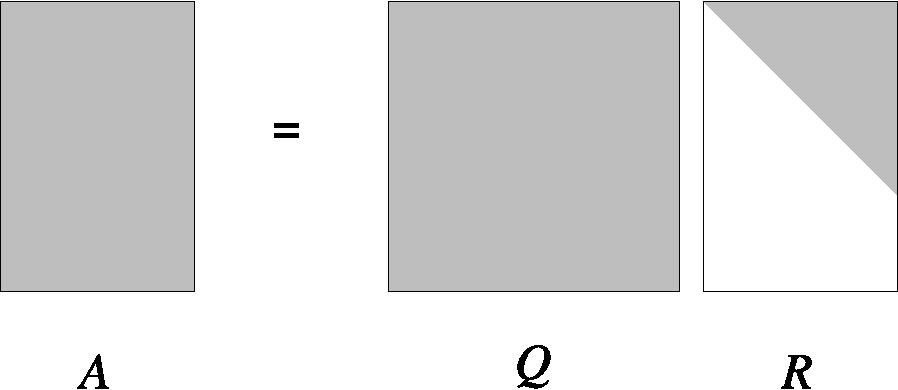
\includegraphics[width=.5\textwidth]{img/full-qr-factorization-1.pdf}
    \caption{Full QR Factorization.}
\end{figure}

\highspace
Let $A$ be an $m \times n$ matrix. The \textbf{reduced QR factorization} of $A$ is the factorization $A = \widehat{Q}\widehat{R}$, where:
\begin{itemize}
    \item $\widehat{Q}$ is $m \times m$
    \item $\widehat{R}$ is $m \times n$ upper-trapezoidal
\end{itemize}
\begin{figure}[!htp]
    \centering
    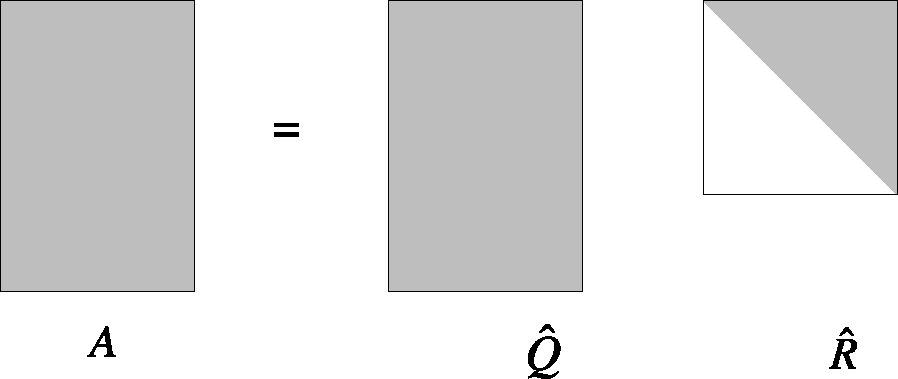
\includegraphics[width=.5\textwidth]{img/reduced-qr-factorization-1.pdf}
    \caption{Reduced QR Factorization.}
\end{figure}

\noindent
Every matrix $A \in \mathbb{C}^{m \times n}$ ($m \ge n$) has a \textbf{full QR factorization and a reduced QR factorization}. Also, every $A$ of \textbf{full rank has a unique reduced QR factorization} with $r_{jj} > 0$, $j = 1, \dots, n$.

\newpage

\begin{flushleft}
    \textcolor{Green3}{\faIcon{question-circle} \textbf{What is Gram-Schmidt orthogonalization and why is it important?}}
\end{flushleft}
After a long mathematical introduction to the full and reduced QR factorization methods, the question is \emph{how can we apply this in practice}? Well, finding a special set of vectors that satisfies some properties cannot be very easy. Fortunately, \definition{Gram-Schmidt orthogonalization} is one of the primary \textbf{methods used to find the orthogonal (or orthonormal) vectors} necessary for QR factorization.

\highspace
The Gram-Schmidt orthogonalization takes as:
\begin{itemize}
    \item \textbf{Input}. A set of vectors (typically the columns of the matrix $A$).
    
    \item \textbf{Output}. An orthogonal set of vectors, which can then be normalized to form an orthonormal set.
\end{itemize}

\highspace
Mathematically, the Gram-Schmidt orthogonalization works as follows. Given the columns of $A$ $\mathbf{a}_{1}, \mathbf{a}_{2}, \dots, \mathbf{a}_{n}$; find new $\mathbf{q}_{j}$ (the $j$-th column of $\widehat{Q}$) orthogonal to $\mathbf{q}_{1}, \dots, \mathbf{q}_{j-1}$ by subtracting components along previous vectors:
\begin{equation*}
    \mathbf{w}_{j} = \mathbf{a}_{j} - \displaystyle\sum_{k=1}^{j-1} \left(\overline{\mathbf{q}}_{k}^{T}\mathbf{a}_{j}\right)\mathbf{q}_{k}
\end{equation*}
Normalize to get $\mathbf{q}_{j} = \dfrac{\mathbf{w}_{j}}{\left|\left|\mathbf{w}_{j}\right|\right|}$, we then obtain a reduced QR factorization with:
\begin{equation}
    r_{ij} = \overline{\mathbf{q}}_{i}^{T}\mathbf{a}_{j} \hspace{2em} i \ne j
\end{equation}
And:
\begin{equation*}
    r_{jj} = \left|\left|\mathbf{a}_{j} - \displaystyle\sum_{i=1}^{j-1} r_{ij}\mathbf{q}_{i}\right|\right|
\end{equation*}
Since the previous equation $r_{ij}$ is numerically unstable because it is too sensitive to rounding errors, the following modification ensures more stability. The previous one is called \definition{Classical Gram-Schmidt (CGS, or simply GS)}, and the following one is called \definition{Classical Gram-Schmidt (CGS, or simply GS)}:
\begin{equation}
    r_{ij} = \overline{\mathbf{q}}_{i}^{T}\mathbf{w}_{j}
\end{equation}
    \subsubsection{Schur decomposition applied to QR algorithm}

Instead of analyzing the classical QR algorithm, which is very general and applicable to any mathematical problem, here we present the powerful \definitionWithSpecificIndex{Schur decomposition}{Schur decomposition applied to QR algorithm}, which is applied with the aim of finding a QR decomposition.

\highspace
\begin{flushleft}
    \textcolor{Green3}{\faIcon{question-circle} \textbf{Why do we need a variant of the QR decomposition algorithm?}}
\end{flushleft}
Before presenting and explaining how to apply it, we think that the motivations are fundamental:
\begin{itemize}
    \item \emph{What is the purpose of using the QR algorithm with the Schur variant?} To transform a matrix into an upper triangular form with eigenvalues on the diagonal.
    
    \item \emph{And why should this be useful? We could get the same result using the theoretical QR decomposition (e.g. Gram-Schmidt).} Obviously, but the Schur decomposition provides \textbf{more numerical stability}. In addition, it is very useful for analyzing eigenvalues and eigenvectors, and it simplifies the computation of matrix functions.
    
    \item \emph{So the Schur decomposition is the best! We will only use that.} Not at all. After explaining the algorithm, we will see why there are other better alternatives.
\end{itemize}

\highspace
\begin{flushleft}
    \textcolor{Red2}{\faIcon{exclamation-triangle} \textbf{Required prerequisites}}
\end{flushleft}
\begin{itemize}
    \item \textbf{Schur decomposition} is a mathematical concept used to transform a square matrix into a quasi-upper triangular form. If $A \in \mathbb{C}^{n \times n}$ then there is a unitary matrix $U \in \mathbb{C}^{n \times n}$ such that:
    \begin{equation*}
        U^{H} A U = T
    \end{equation*}
    And $U$ is upper triangular. The diagonal elements of $T$ are the eigenvalues of $A$. The Schur vectors are $U = \left|\mathbf{u}_{1}, \mathbf{u}_{2}, \dots, \mathbf{u}_{n}\right|$ and they are in general not eigenvectors.

    \item The $k$-th column of $U^{H} A U = T$ read:
    \begin{equation*}
        A\mathbf{u}_{k} = \lambda_{k}\mathbf{u}_{k} + \displaystyle\sum_{i=1}^{k-1} t_{ik}\mathbf{u}_{i}
    \end{equation*}
    That is:
    \begin{equation*}
        A\mathbf{u}_{k} \in \mathrm{span}\left\{\mathbf{u}_{1}, \dots, \mathbf{u}_{k}\right\} \hspace{2em} \forall k
    \end{equation*}
    The first \textbf{Schur vector} $\mathbf{u}_{1}$ is an eigenvector of $A$. The first $k$ Schur vectors $\mathbf{u}_{1}, \dots, \mathbf{u}_{k}$ form an invariant subspace for $A$. The Schur decomposition is not unique.
\end{itemize}

\newpage

\begin{flushleft}
    \textcolor{Green3}{\faIcon{tools} \textbf{Algorithm}}
\end{flushleft}
\textbf{Goal}: let $A \in \mathbb{C}^{n \times n}$, the QR algorithm computes an upper triangular matrix $T$ and a unitary matrix $U$ such that $A = UTU^{H}$ is the Schur decomposition of $A$.
\begin{enumerate}
    \item \textbf{Initialization}. $A$ is the \emph{original matrix} we start with; at the beginning, the initial guess $A^{\left(0\right)}$ is equal to the original $A^{\left(0\right)} = A$. It is transformed iteratively by the QR decompositions and updates. Meanwhile, $U$ is the \emph{accumulation of orthogonal transformations} applied to $A$. Initially, $U$ is set to the identity matrix $U^{\left(0\right)} = I$.
    \begin{equation*}
        \begin{array}{rcl}
            A^{\left(0\right)} &=& A \\ [.3em]
            U^{\left(0\right)} &=& I
        \end{array}
    \end{equation*}

    \item \textbf{Iteration}. For each $k \ge 1$:
    \begin{enumerate}
        \item \textbf{QR Decomposition}. Decompose the matrix $A^{\left(k-1\right)}$ into the product of an orthogonal matrix $Q^{\left(k\right)}$ and an upper triangular matrix $R^{\left(k\right)}$:
        \begin{equation*}
            A^{\left(k-1\right)} = Q^{\left(k\right)} R^{\left(k\right)}
        \end{equation*}

        \item \textbf{Update the matrix $A$} to be used in next iteration by multiplying $R^{\left(k\right)}$ and $Q^{\left(k\right)}$:
        \begin{equation*}
            A^{\left(k\right)} = R^{\left(k\right)} Q^{\left(k\right)}
        \end{equation*}

        \item \textbf{Update the Transformations matrix $U$} to keep track of the cumulative orthogonal transformations:
        \begin{equation*}
            U^{\left(k\right)} = U^{\left(k-1\right)} Q^{\left(k\right)}
        \end{equation*}
    \end{enumerate}

    \item \textbf{Repeat until we meet a specific stopping criteria}.
    
    \item \textbf{Results}. If a certain stopping criterion is met, we have the upper triangular matrix $A^{\left(k\right)}$ and the orthogonal matrix $U^{\left(k\right)}$. The Schur decomposition gives us an important result:
    \begin{equation*}
        T = A^{\left(k\right)} \: \land \: U^{\left(k\right)} = U \: \Longrightarrow \: A = U T U^{H} \: \equiv \: U^{H} A U = T
    \end{equation*}
\end{enumerate}
About the convergence, we need to show some interesting details. Let us assume that all the eigenvalues are isolated:
\begin{equation*}
    \left|\lambda_{1}\right| > \left|\lambda_{2}\right| > \dots > \left|\lambda_{n}\right|
\end{equation*}
Then the elements of $A^{\left(k\right)}$ below the diagonal converge to zero:
\begin{equation*}
    \lim\limits_{k \rightarrow \infty} a_{ij}^{\left(k\right)} = 0 \hspace{2em} \forall i > j
\end{equation*}
Moreover, it can be shown that:
\begin{equation*}
    a_{ij}^{\left(k\right)} = O\left(
        \left|\dfrac{\lambda_{i}}{\lambda_{i}}\right|^{k}
    \right) \hspace{2em} i > j
\end{equation*}
Thus, \textbf{\underline{convergence} is low when the eigenvalues are close}.

\highspace
\begin{flushleft}
    \textcolor{Red2}{\faIcon{dollar-sign} \textbf{How much does it cost?}}
\end{flushleft}
The QR algorithm enhanced with Schur decomposition is powerful for finding eigenvalues and eigenvectors, but the \textbf{high iteration cost} of $\approx n^{3}$ operations is a tradeoff for its robustness and accuracy.

\highspace
\begin{flushleft}
    \textcolor{Green3}{\faIcon{network-wired} \textbf{Can it be parallelized?}}
\end{flushleft}
The Schur decomposition applied to the QR algorithm is \textbf{difficult} to parallelize due to its sequential dependencies.
    \subsubsection{Hessenberg applied to QR algorithm}

A matrix $H \in \mathbb{C}^{n \times n}$ is called a \definition{Hessenberg matrix} if its elements below the lower off-diagonal are zero:
\begin{equation*}
    h_{ij} = 0 \hspace{2em} i > j + 1
\end{equation*}
For example:
\begin{equation*}
    H = \begin{bmatrix}
        * & * & * & * & * & * \\
        * & * & * & * & * & * \\
        0 & * & * & * & * & * \\
        0 & 0 & * & * & * & * \\
        0 & 0 & 0 & * & * & * \\
        0 & 0 & 0 & 0 & * & *
    \end{bmatrix}
\end{equation*}

\highspace
\begin{flushleft}
    \textcolor{Green3}{\faIcon{question-circle} \textbf{Why do we use Hessenberg?}}
\end{flushleft}
Apply the QR method to a Hessenberg matrix can be decrease the number of operations from $n^{3}$ (Schur decomposition, page \pageref{subsubsection: Schur decomposition applied to QR algorithm}) to $n^{2}$ \textbf{operations}.

\highspace
\begin{flushleft}
    \textcolor{Green3}{\faIcon{tools} \textbf{Algorithm}}
\end{flushleft}
\textbf{Goal}: compute a Hessenberg matrix $H$ and an orthogonal matrix $U$ such that $A = UHU^{H}$ is the QR decomposition of $A$. Such  a reduction can be done with a finite number of operations.
\begin{enumerate}
    \item \textbf{Initial Transformation to Hessenberg Form}. Take as input the matrix $A$, we convert $A$ to a Hessenberg matrix $H$ using similarity transformations techniques.
    
    \item \textbf{Initial guess and initial accumulation of orthogonal transformations}. The first guess is the first Hessenberg form we got from the previous step, and for the $U^{\left(0\right)}$ we take the identity as always:
    \begin{equation*}
        \begin{array}{rcl}
            H^{\left(0\right)} &=& H \\ [.3em]
            U^{\left(0\right)} &=& I
        \end{array}
    \end{equation*}

    \item \textbf{Iteration}. For each $k \ge 1$:
    \begin{enumerate}
        \item \textbf{Hessenberg QR Decomposition}. Decompose the matrix $H^{\left(k-1\right)}$ into the product of an orthogonal matrix $Q^{\left(k\right)}$ and an upper triangular matrix $R^{\left(k\right)}$:
        \begin{equation*}
            H^{\left(k-1\right)} = Q^{\left(k\right)} R^{\left(k\right)}
        \end{equation*}

        \item \textbf{Update the Hessenberg matrix $H$} to be used in next iteration by multiplying $R^{\left(k\right)}$ and $Q^{\left(k\right)}$:
        \begin{equation*}
            H^{\left(k\right)} = R^{\left(k\right)} Q^{\left(k\right)}
        \end{equation*}

        \item \textbf{Update the Transformations matrix $U$} to keep track of the cumulative orthogonal transformations:
        \begin{equation*}
            U^{\left(k\right)} = U^{\left(k-1\right)} Q^{\left(k\right)}
        \end{equation*}
    \end{enumerate}

    \item \textbf{Repeat until we meet a specific stopping criteria}.
    
    \item \textbf{Results}. If a certain stopping criterion is met, we have the upper triangular matrix $H^{\left(k\right)}$ and the orthogonal matrix $U^{\left(k\right)}$. The Schur decomposition using the Hessenberg matrix gives us an important result:
    \begin{equation*}
        H = H^{\left(k\right)} \: \land \: U^{\left(k\right)} = U \: \Longrightarrow \: A = U H U^{H} \: \equiv \: U^{H} A U = H
    \end{equation*}
\end{enumerate}

\highspace
\begin{flushleft}
    \textcolor{Red2}{\faIcon{dollar-sign} \textbf{How much does it cost?}}
\end{flushleft}
As we have already said, the Hessenberg matrix \textbf{reduces the computational cost to} $n^{2}$, which is more competitive than the Schur decomposition ($n^{3}$).

\highspace
\begin{flushleft}
    \textcolor{Green3}{\faIcon{network-wired} \textbf{Can it be parallelized?}}
\end{flushleft}
As we have seen with the other QR methods, parallelization is still \textbf{difficult}. It can be achieved with some very optimized libraries, but in general it is complicated due to its dependencies.
    \subsection{Lanczos method}

The \definition{Lanczos algorithm} is an iterative method for \textbf{finding the eigenvalues and eigenvectors} of a large, sparse, symmetric (or Hermitian) matrix. It's particularly \textbf{useful for computing the extremal (largest or smallest) eigenvalues and their corresponding eigenvectors}. The algorithm generates a sequence of vectors, called \emph{Lanczos vectors}, which are used to form a tridiagonal matrix that approximates the original matrix. Finally, this method is also used to \textbf{find a low-rank approximation} of the input matrix; by low-rank, we mean a \textbf{technique} used in numerical linear algebra to simplify a matrix while preserving its most important properties. It is particularly useful \textbf{for reducing the complexity of large data sets, compressing information, and speeding up computations}.

\begin{flushleft}
    \textcolor{Green3}{\faIcon{check} \textbf{Good prerequisites of the matrix}}
\end{flushleft}
Some good prerequisites necessary to get the best performance with the Lanczos algorithm are:
\begin{itemize}
    \item Sparse matrix;
    \item Symmetric (or Hermitian) matrix;
    \item Square matrix, then a size of $n \times n$.
\end{itemize}

\highspace
\begin{flushleft}
    \textcolor{Green3}{\faIcon{square-root-alt} \textbf{Mathematical point of view}}
\end{flushleft}
Let a symmetric matrix $A$ of size $n \times n$, the Lanczos algorithm is based on computing the following decomposition of $A$:
\begin{equation}
    A = QTQ^{T}
\end{equation}
Where $Q$ is an orthonormal basis of vectors $\mathbf{q}_{1}, \dots, \mathbf{q}_{n}$ and $T$ is tri-diagonal:
\begin{equation*}
    Q = \left[\mathbf{q}_{1}, \mathbf{q}_{2}, \dots, \mathbf{q}_{n}\right] \hspace{2em} T = \begin{bmatrix}
        \alpha_{1} & \beta_{1} & 0 & \cdots & 0 \\
        \beta_{1} & \alpha_{2} & \beta_{2} & \cdots & 0 \\
        0 & \ddots & \ddots & \ddots & 0 \\
        0 & \ddots & \ddots & \ddots & \beta_{n-1} \\
        0 & \cdots & 0 & \beta_{n-1} & \alpha_{n}
    \end{bmatrix}
\end{equation*}
The \textbf{decomposition always exists} and is \textbf{unique} if $\mathbf{q}_{1}$ was specified. 

Since we know that $T = Q^{T} A Q$ which gives:
\begin{equation*}
    \alpha_{k} = \mathbf{q}_{k}^{T} A \mathbf{q}_{k} \hspace{2em} \beta_{k} = \mathbf{q}_{k+1}^{T} A \mathbf{q}_{k}
\end{equation*}
The full decomposition is obtained by imposing $AQ = QT$:
\begin{gather*}
    \left[A\mathbf{q}_{1}, A\mathbf{q}_{2}, \dots, A\mathbf{q}_{n}\right] = \\
    [
        \underbrace{\alpha_{1}\mathbf{q}_{1} + \beta_{1}\mathbf{q}_{2}}_{\text{1st row}}, \:
        \underbrace{\beta_{1}\mathbf{q}_{1} + \alpha_{2}\mathbf{q}_{2} + \beta_{2}\mathbf{q}_{3}}_{\text{\text{2nd row}}}, \:
        \dots, \:
        \underbrace{\beta_{n-1}\mathbf{q}_{n-1} + \alpha_{n}\mathbf{q}_{n}}_{n \text{ row}}
    ]
\end{gather*}

\newpage

\begin{flushleft}
    \textcolor{Green3}{\faIcon{tools} \textbf{Algorithm}}
\end{flushleft}
Note that at iteration $k$, the algorithm generates intermediate matrices $Q_{k}$ and $T_{k}$ satisfying $T_{k} = Q_{k}^{T} A Q_{k}$.
\begin{enumerate}
    \item \textbf{Residual, Lanczos vector and scalar initialization}. We set the residual to the value of the lanczos vector $\mathbf{q}_{1}$ which is set randomly; the Lanczos vector is set to zero and finally the scalar $\beta$ is set to one.
    \begin{equation*}
        \mathbf{r}_{0} = \mathbf{q}_{1}
        \hspace{2em}
        \mathbf{q}_{0} = \mathbf{0}
        \hspace{2em}
        \beta = 1
    \end{equation*}

    \item \textbf{Iteration}. For each $k = 1, \dots, n$:
    \begin{enumerate}
        \item \textbf{Check if the previously calculated $\beta$ is zero}. If zero, stop the algorithm, otherwise continue the iteration.

        \item \textbf{Compute Lanczos vector $\mathbf{q}_{k}$}:
        \begin{equation*}
            \mathbf{q}_{k} = \dfrac{\mathbf{r}_{k-1}}{\beta_{k-1}}
        \end{equation*}

        \item \textbf{Compute scalar $\alpha_{k}$}:
        \begin{equation*}
            \alpha_{k} = \mathbf{q}_{k}^{T} \mathbf{A} \mathbf{q}_{k}
        \end{equation*}

        \item \textbf{Compute the residual $\mathbf{r}_{k}$}:
        \begin{equation*}
            \mathbf{r}_{k} = \left(\mathbf{A} - \alpha_{k}\right)\mathbf{q}_{k} - \beta_{k-1}\mathbf{q}_{k-1}
        \end{equation*}

        \item \textbf{Compute scalar $\beta_{k}$}:
        \begin{equation*}
            \beta_{k} = \left|\mathbf{r}_{k}\right|
        \end{equation*}
    \end{enumerate}

    \item \textbf{Results}. It produces the tridiagonal symmetric matrix $T$ that is an approximation of the original matrix $A$ and the orthonormal basis $Q_{k}$.
\end{enumerate}
At iteration $k$, the $k$-th Lanczos vector $\mathbf{q}_{k}$ is proven to maximize the left hand side of:
\begin{equation*}
    \underset{\mathbf{y} \ne \mathbf{0}}{\max} \dfrac{
        \mathbf{y}^{T} \left(Q_{k}^{T}A Q_{k}\right) \mathbf{y}
    }{
        \mathbf{y}^{T} \mathbf{y}
    }
    =
    \lambda_{1}\left(T_{k}\right) \le \lambda_{1}\left(A\right) = \lambda_{1}\left(T\right)
\end{equation*}
And to simultaneously minimize the left hand side of:
\begin{equation*}
    \underset{\mathbf{y} \ne \mathbf{0}}{\min} \dfrac{
        \mathbf{y}^{T} \left(Q_{k}^{T}A Q_{k}\right) \mathbf{y}
    }{
        \mathbf{y}^{T} \mathbf{y}
    }
    =
    \lambda_{n}\left(T_{k}\right) \le \lambda_{n}\left(A\right) = \lambda_{n}\left(T\right)
\end{equation*}
Where:
\begin{itemize}
    \item $\lambda_{1}\left(A\right)$ is the \textbf{\emph{maximum} eigenvalue} of $A$;
    \item $\lambda_{n}\left(A\right)$ is the \textbf{\emph{minimum} eigenvalue} of $A$.
\end{itemize}

\newpage

\begin{flushleft}
    \textcolor{Red2}{\faIcon{dollar-sign} \textbf{How much does it cost?}}
\end{flushleft}
Although the algorithm is quite complex to understand, the computational cost is very competitive. If we respect all the prerequisites that we have said, then for \textbf{large}, \textbf{symmetric}, \textbf{sparse} and \textbf{square matrices}, the primary cost is proportional to the \textbf{number of non-zero elements} in the matrix. Thus, the cost of each iteration is only $\approx \nnz\left(A\right)$ \textbf{operations} (where $A$ is the input matrix).

\highspace
The reasoning changes for \textbf{dense matrices}, although still feasible, the cost can be higher due to the $\approx n^{2}$ \textbf{operations}.

\highspace
\begin{flushleft}
    \textcolor{Green3}{\faIcon{network-wired} \textbf{Can it be parallelized?}}
\end{flushleft}
The Lanczos method is widely used in practice, and obviously it \textbf{fits very well with parallel patterns}. The Lanczos parallelization focuses on matrix-vector multiplication and orthogonalization steps. If the reader wants to delve deeper into this parallelization, we suggest an interesting scientific paper:
\begin{center}
    \href{https://link.springer.com/chapter/10.1007/978-3-642-11322-2_25}{Parallelization of the Lanczos Algorithm on Multi-core Platforms} \qrcode{https://link.springer.com/chapter/10.1007/978-3-642-11322-2_25}

    \highspace
    \href{https://cse.iitkgp.ac.in/~abhij/publications/ParLanczos10.pdf}{Link to the paper} \hspace{2em} \qrcode{https://cse.iitkgp.ac.in/~abhij/publications/ParLanczos10.pdf}
\end{center}

    %%%%%%%%%%%%%%%%%%%%%%%%%%%%%%%%%%%%%%%%%%%%%%%%%%%%%%%%%%%%%%%
    % Numerical methods for overdetermined linear systems and SVD %
    %%%%%%%%%%%%%%%%%%%%%%%%%%%%%%%%%%%%%%%%%%%%%%%%%%%%%%%%%%%%%%%
    \section{Numerical methods for overdetermined linear systems and SVD}

\subsection{Overdetermined systems and Least Squares}

An \definition{Overdetermined linear system} is a \textbf{system of linear equations in which there are more equations than unknowns}. In other words, there are more constraints than variables, which often makes it \emph{impossible to satisfy all the equations simultaneously}. This often happens in practical applications where we have more measurements or constraints than variables.

\highspace
The solution method is \definitionWithSpecificIndex{Least Squares}{Least Squares method}; it finds an approximate \textbf{solution by minimizing the sum of the squares of the residuals} (the differences between the left and right sides of the equations). A practical implementation is Singular Value Decomposition (SVD).

\highspace
\begin{flushleft}
    \textcolor{Green3}{\faIcon{square-root-alt} \textbf{Mathematical point of view}}
\end{flushleft}
The mathematical problem reads: given $A \in \mathbb{R}^{m \times n}$, with $m \ge n$ and $\mathbf{b} \in \mathbb{R}^{m}$, find $\mathbf{x} \in \mathbb{R}^{n}$ such that: $A\mathbf{x} = \mathbf{b}$.

\begin{figure}[!htp]
    \centering
    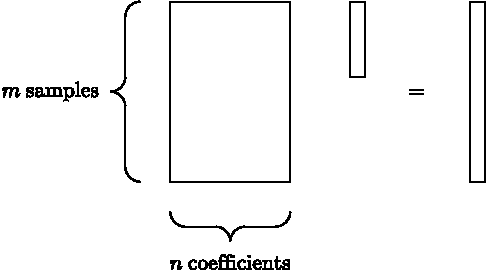
\includegraphics[width=.6\textwidth]{img/overdetermined-linear-systems-1.pdf}
\end{figure}

\noindent
Note that the above problems generally have no solution unless the right side $\mathbf{b}$ is an element of $\mathrm{range}\left(A\right)$ (all possible linear combinations of the columns of $A$). So the basic approach is to look for a $\mathbf{x}$ that makes $A\mathbf{x}$ \dquotes{close} to $\mathbf{b}$.

\highspace
We compute the solution using least-squares. Given $A \in \mathbb{R}^{m \times n}$, $m \ge n$, we say that $\mathbf{x}^{*} \in \mathbb{R}^{n}$ is a solution of the linear system $A\mathbf{x} = \mathbf{b}$ in the least-squares sense if:
\begin{equation}
    \Phi\left(\mathbf{x}^{*}\right) = \underset{\mathbf{y} \in \mathbb{R}^{n}}{\min} \Phi\left(\mathbf{y}\right)
\end{equation}
Where:
\begin{equation}
    \Phi\left(\mathbf{y}\right) = {\left|\left|A\mathbf{y} - \mathbf{b}\right|\right|}_{2}^{2}
\end{equation}
The problem thus consists of minimizing the Euclidean norm of the residual. The \textbf{solution} $\mathbf{x}^{*}$ can be \textbf{found by imposing the condition that the gradient of the function} $\Phi\left(\cdot\right)$ \textbf{must be equal to zero at} $\mathbf{x}^{*}$. From the definition we have:
\begin{equation*}
    \begin{array}{rcl}
        \Phi\left(\mathbf{y}\right) &=& \left(A\mathbf{y} - \mathbf{b}\right)^{T}\left(A\mathbf{y} - \mathbf{b}\right) \\ [.3em]
        %
        &=& \mathbf{y}^{T}A^{T}A\mathbf{y} - 2\mathbf{y}^{T} A \mathbf{b} + \mathbf{b}^{T}\mathbf{b}
    \end{array}
\end{equation*}
Therefore:
\begin{equation*}
    \nabla\Phi\left(\mathbf{y}\right) = 2A^{T} A \mathbf{y} - 2A^{T}\mathbf{b}
\end{equation*}
From which it follows that $\mathbf{x}^{*}$ must be the solution of the square system:
\begin{equation}
    A^{T}A\mathbf{x}^{*} = A^{T}\mathbf{b}
\end{equation}

\highspace
The system of normal equations is nonsingular if $A$ has \textbf{full rank} and, in such a case, the least-squares \textbf{solution exists and is unique}.

\begin{theorem}
    Let $A \in \mathbb{R}^{m \times n}$, with $m \ge n$, be a full rank matrix. Then the \textbf{unique solution} in the least-square sense $\mathbf{x}^{*}$ of $A\mathbf{x}^{*} = \mathbf{b}$ is given by $\mathbf{x}^{*} = \widehat{R}^{-1}\widehat{Q}^{T}\mathbf{b}$, where $\widehat{R} \in \mathbb{R}^{n \times n}$ and $\widehat{Q} \in \mathbb{R}^{m \times n}$ are the matrices of the reduced QR factorization of A. Moreover, the minimum of $\Phi\left(\cdot\right)$ is given by:
    \begin{equation*}
        \Phi\left(\mathbf{x}^{*}\right) = \displaystyle\sum_{i = n+1}^{m} \left[\left(Q^{T}b\right)_{i}\right]^{2}
    \end{equation*}
\end{theorem}

\noindent
If $A$ has full rank, then since the solution exists in the least squares sense and is unique, it must necessarily have \textbf{minimal Euclidean norm}:
\begin{equation}\label{eq: minimal Euclidean norm}
    {\left|\left|A \mathbf{x}^{*} - \mathbf{b}\right|\right|}_{2}^{2} \le \underset{\mathbf{x} \in \mathbb{R}^{n}}{\min} {\left|\left|A\mathbf{x} - \mathbf{b}\right|\right|}_{2}^{2}
\end{equation}

\highspace
In other words, given an overdetermined system $A\mathbf{x} = \mathbf{b}$, the least squares method finds $\mathbf{x}$ that minimizes the quantity ${\left|\left|A\mathbf{x} - \mathbf{b}\right|\right|}_{2}^{2}$. These problems can be solved using the SVD method.

    \subsection{Singular Value Decomposition (SVD)}

\definition{Singular Value Decomposition (SVD)} is a factorization of a matrix into three other matrices. For any $m \times n$ matrix $A$, the SVD is given by:
\begin{equation}\label{eq: singular value decomposition}
    A = U \Sigma V^{T}
\end{equation}
It \textbf{provides a solution to Least Squares techniques}. Where:
\begin{itemize}
    \item $U$ is an $m \times m$ orthogonal matrix, called \textbf{left singular vectors}. These vectors form an \emph{orthonormal basis} for the column space of $A$.

    \item $\Sigma$ is a $m \times n$ diagonal matrix with non-negative real numbers on the diagonal, called \textbf{singular values}. These values are sorted in \textbf{descending order} (from largest to smallest), and the number of values is guaranteed by the minimum between the number of columns and the number of rows; if $A$ is $m \times n$, there are $\min\left(m,n\right)$ singular values.
    
    These values are important because keeping only the largest singular values can reduce the dimensions of the data while preserving important features. It also compresses the image, if the matrix represents an image, and filters out noise.

    \item $V$ is an $n \times n$ orthogonal matrix, called \textbf{right singular vectors}. These vectors form an orthonormal basis for the row space of $A$.
\end{itemize}

\begin{theorem}
    Let $A \in \mathbb{R}^{m \times n}$. There exist two orthogonal matrices $U \in \mathbb{R}^{m \times m}$ and $V \in \mathbb{R}^{n \times n}$ such that:
    \begin{equation}\label{eq: SVD theorem}
        U^{T} A V = \Sigma = \mathrm{diag}\left(\sigma_{1}, \dots, \sigma_{p}\right) \in \mathbb{R}^{m \times n}
    \end{equation}
    With $p = \min\left(m, n\right)$ and $\sigma_{1} \ge \dots \ge \sigma_{p} \ge 0$.
\end{theorem}

\noindent
This method is a robust mathematical tool commonly employed in machine learning for tasks such as dimensionality reduction, data compression and feature extraction. It is especially effective in handling high-dimensional datasets, helping to lower computational complexity and enhance the efficiency of machine learning algorithms.
\begin{itemize}
    \item[\ding{51}] Singular Value Decomposition (SVD) is an \textbf{alternative to Eigenvalue Decomposition}, which is \textbf{generally better} for rank-deficient and ill-conditioned matrices.
    \item[\ding{51}] Computing the \textbf{SVD is always numerically stable} for any matrix but is typically \textbf{more expensive than other decompositions}.
    \item[\ding{51}] SVD can be used to \textbf{compute low-rank approximations} to a matrix via Principal Component Analysis (PCA has many practical applications, and usually large sparse matrices arise).
\end{itemize}

\newpage
\begin{flushleft}
    \textcolor{Green3}{\faIcon{square-root-alt} \textbf{SVD features}}
\end{flushleft}
\begin{itemize}
    \item If $A$ is a real-valued matrix, $U$ and $V$ will also be real-valued and in the equation \ref{eq: SVD theorem}, $U^{T}$ must be written instead of $U^{H}$.

    \item The singular values holds:
    \begin{equation}
        \sigma_{i}\left(A\right) = \sqrt{\lambda_{i}\left(A^{T} A\right)} \hspace{2em} i = 1, \dots, p
    \end{equation}

    \item Since $AA^{T}$ and $A^{T}A$ are symmetric matrices, the columns of $U$ turn out to be the eigenvectors of $A^{T}A$ and, therefore, they are not uniquely defined. The same holds for the columns of $V$, which are the right singular vectors of $A$.

    \item As far as the $\mathrm{rank}\left(A\right)$ is concerned, if:
    \begin{equation*}
        \sigma_{1} \ge \sigma_{2} \ge \dots \ge \sigma_{r} > 0 \hspace{2em} \text{and} \hspace{2em} \sigma_{r+1} = \dots = \sigma_{p} = 0
    \end{equation*}
    Then the rank of $A$ is $r$, the kernel of $A$ is the span of the column vectors of $V$, $\left\{\mathbf{v}_{r+1}, \dots, \mathbf{v}_{n}\right\}$, and the range of $A$ is the span of the column vectors of $U$, $\left\{\mathbf{u}_{1}, \dots, \mathbf{u}_{p}\right\}$.
\end{itemize}

\highspace
\begin{flushleft}
    \textcolor{Green3}{\faIcon{bookmark} \textbf{Generalized inverse}}
\end{flushleft}
The \definition{Generalized Inverse of a matrix} $A$ is a matrix that can provide \textbf{solutions to systems of linear equations} that may not have unique solutions or may not be solvable using the regular inverse (such as least squares problems). There are different types of generalized inverses, but one of the most commonly used is the \textbf{Moore-Penrose pseudo-inverse}, denoted as $A^{\dagger}$.

\begin{definitionbox}[: Moore-Penrose]
    Suppose that $A \in \mathbb{R}^{m \times n}$ has rank equal to $r$ and that it admits a SVD of the type $U^{T} A V = \Sigma$. The matrix:
    \begin{equation}
        A^{\dagger} = V \Sigma^{\dagger} U^{T}
    \end{equation}
    Is called the \definition{Moore-Penrose pseudo-inverse matrix}, being:
    \begin{equation}
        \Sigma^{\dagger} = \mathrm{diag}\left\{
            \dfrac{1}{\sigma_{1}},
            \dots,
            \dfrac{1}{\sigma_{p}},
            0,
            \dots,
            0
        \right\}
    \end{equation}
    The matrix $A^{\dagger}$ is also called the \textbf{generalized inverse of $A$}. Also, if $n = m = \mathrm{rank}\left(A\right)$, then $A^{\dagger} = A^{-1}$.
\end{definitionbox}

\noindent
The Moore-Penrose pseudo-inverse matrix is used in the SVD method to \textbf{solve the overdetermined systems} using the least squares technique.

\begin{theorem}
    Let $A \in \mathbb{R}^{m \times n}$ with SVD given by $A = U \Sigma V^{T}$. Then the unique solution to the equation \ref{eq: minimal Euclidean norm} is:
    \begin{equation}
        \mathbf{x}^{*} = A^{\dagger}\mathbf{b}
    \end{equation}
    Where $A^{\dagger}$ is the pseudo-inverse of $A$.
\end{theorem}

\highspace
\begin{flushleft}
    \textcolor{Green3}{\faIcon{tools} \textbf{How to calculate SVD}}
\end{flushleft}
The \definition{Householder reflection} (or Householder transformation) is a method used in linear algebra to zero out the subdiagonal elements of a matrix, transforming it into a simpler form such as an upper triangular matrix or a bidiagonal matrix. 

\highspace
The use of Householder reflections is \textbf{recommended} because they provide a \textbf{numerically stable and efficient way to reduce a matrix to bidiagonal form}. This reduction makes the subsequent \textbf{steps of the SVD calculation easier and more computationally efficient}.
\begin{equation*}
    U_{1}^{T}AV_{1} = B = \begin{bmatrix}
        d_{1} & f_{1} & \cdots & \cdots & 0_{n} \\
        0 & d_{2} & f_{2} & \cdots & \vdots \\
        \vdots & \vdots & \ddots & \ddots & \vdots \\
        \vdots & \vdots & \vdots & d_{n-1} & f_{n-1} \\
        0 & 0 & \cdots & 0 & d_{n}
    \end{bmatrix}
\end{equation*}
It follows that $T = B^{T}B$ is symmetric and tridiagonal. We could then apply the QR algorithm directly to $B$.

    %%%%%%%%%%%%%%%%%%%%%
    % Multigrid methods %
    %%%%%%%%%%%%%%%%%%%%%
    \section{Multigrid methods}

\subsection{Idea of MG methods}

The \definition{multigrid (MG) methods} are efficient \textbf{algorithms for solving large systems of linear equations}, particularly those \textbf{arising from the discretization of partial differential equations} (PDEs). They're especially useful for problems that exhibit behavior on multiple scales.

\highspace
A multigrid (MG) method is an iterative algorithm of the form:
\begin{equation}
    \mathbf{x}^{\left(k+1\right)} = \mathrm{MG}\left(\mathbf{x}^{\left(k\right)}\right) \hspace{2em} k \ge 0
\end{equation}
For solving the (typically) sparse linear systems of equations stemming from the numerical discretization of differential equations. The \textbf{MG methods are based on}:
\begin{itemize}
    \item \textbf{\emph{Hierarchy of levels}} (associated with a hierarchy of discretization):
    \begin{itemize}
        \item \textbf{\underline{Fine Grid}}. The finest grid \textbf{captures the most detailed features} of the problem. This is where the original problem is defined and where the final solution needs to be accurate.
        
        \item \textbf{\underline{Coarse Grids}}. They are lower resolution versions of the fine grid. They \textbf{capture broader}, \textbf{large-scale features} of the problem. The coarser the grid, the \textbf{fewer the details}, but \textbf{computations are cheaper and faster}.
        
        Coarse grids help in correcting the errors that are hard to eliminate on finer grids due to their global nature.
    \end{itemize}

    \item \textbf{\emph{MG cycles}} reduce all error components by a fixed amount (bounded well below one), regardless of the dimension $n$ of the system.
\end{itemize}
The \textbf{main idea} of MG is to \textbf{accelerate the convergence of a basic iterative method} by a global correction of the fine grid solution approximation accomplished by solving a coarse problem. The coarse-level problem should be \emph{similar} to the fine grid problem. The cost of (direct) solution of the coarse problem should be negligible compared to the cost of one relaxation sweep on the fine grid.

\highspace
In other words, the main goal of the multigrid method is to speed up the convergence of an iterative method for solving systems of linear equations. This acceleration is achieved by globally correcting the solution approximation on the fine grid by solving a similar problem on a coarser grid.
    \subsection{How it works}

\subsubsection{Computation}

A single \textbf{processor} of the PRAM, at each computation, is \textbf{composed of 5 phases} (carried out in parallel by all the processors):
\begin{enumerate}
    \item \textbf{Reads a value from one of the cells} $X\left(1\right), \dots, X\left(N\right)$
    \item Reads one of the shared memory cells $A\left(1\right), A\left(2\right), \dots$
    \item Performs some internal computation
    \item \textbf{May write into one of the output cells} $Y\left(1\right), Y\left(2\right), \dots$
    \item May write into one of the shared memory cells $A\left(1\right), A\left(2\right), \dots$
\end{enumerate}

\longline

\subsubsection{PRAM Classificiation}

During execution, a subset of processors may remain idle. Also, some processors can read from the same cell at the same time (not really a problem), but they could also try to write to the same cell at the same time (\textbf{write conflict}). For these reasons, PRAMs are classified according to their read/write capabilities (realistic and useful):
\begin{itemize}
    \item \definition{Exclusive Read (ER)}. All processors can simultaneously read from distinct memory locations.
    
    \item \definition{Exclusive Write (EW)}. All processors can simultaneously write to distinct memory locations.
    
    \item \definition{Concurrent Read (CR)}. All processors can simultaneously read from any memory location.

    \item \definition{Concurrent Write (CW)}. All processors can write to any memory location.
    \begin{flushleft}
        \textcolor{Green3}{\faIcon{question-circle} \textbf{But what value is ultimately written?}}
    \end{flushleft}
    It depends on the mode we choose:
    \begin{itemize}
        \item \definition{Priority Concurrent Write}. Processors have priority based on which value is decided, the \textbf{highest priority is allowed to complete write}.

        \item \definition{Common Concurrent Write}. All processors are allowed to complete write \textbf{if and only if all the value to be written are equal}.
        
        Any \textbf{algorithm} for this model has to \textbf{make sure that this condition is satisfied}. \textbf{Otherwise}, the \textbf{algorithm is illegal} and the \textbf{machine state will be undefined}.

        \item \definitionWithSpecificIndex{Arbitrary/Random Concurrent Write}{Arbitrary Concurrent Write}{Random Concurrent Write}. One \textbf{randomly} chosen \textbf{processor is allowed to complete write}.
    \end{itemize}
\end{itemize}

\subsubsection{Strengths of PRAM}

PRAM is attractive and important model for designers of parallel algorithms because:
\begin{itemize}
    \item It is \textbf{natural}. The number of operations executed per one cycle on $P$ processors is at most $P$ (equal to $P$ is the ideal case).

    \item It is \textbf{strong}. Any processor can read/write any shared memory cell in unit time.

    \item It is \textbf{simple}. It abstracts from any communication or synchronization overhead, which makes the complexity and correctness of PRAM algorithm easier.

    \item It can be used as a \textbf{benchmark}. If a problem has no feasible/efficient solution on PRAM, it has no feasible/efficient solution for any parallel machine.
\end{itemize}

\longline

\subsubsection{How to compare PRAM models}

Consider two generic PRAMs, models $A$ and $B$. Model $A$ is \textbf{computationally stronger} than model $B$ ($A \ge B$) \textbf{if and only if} \textbf{any algorithm} written for model $B$ will \textbf{run unchanged} on model $A$ in the \textbf{same parallel time} and with the \textbf{same basic properties}.

\highspace
However, there are some useful metrics that can be used to compare models:
\begin{itemize}
    \item \textbf{Time to solve problem} of \textbf{input size} $n$ on \textbf{\underline{one} processor}, using \textbf{best \underline{sequential} algorithm}:
    \begin{equation}
        T^{*}\left(n\right)
    \end{equation}

    \item \textbf{Time} to solve problem of input size $n$ on \underline{$\mathbf{p}$} \textbf{processors}:
    \begin{equation}
        T_{p}\left(n\right)
    \end{equation}

    \item \textbf{Speedup on $\mathbf{p}$ processors}:
    \begin{equation}
        \mathrm{SU}_{p}\left(n\right) = \dfrac{T^{*}\left(n\right)}{T_{p}\left(n\right)}
    \end{equation}

    \item \textbf{Efficiency}, which is the work done by a processor to solve a problem of input size $n$ divided by the work done by $p$ processors:
    \begin{equation}
        E_{p}\left(n\right) = \dfrac{T_{1}\left(n\right)}{pT_{p}\left(n\right)}
    \end{equation}

    \item \textbf{Shortest run time} on any process $p$:
    \begin{equation}
        T_{\infty}\left(n\right)
    \end{equation}

    \item \textbf{Cost}, equal to processors and time:
    \begin{equation}
        C\left(n\right) = P\left(n\right) \cdot T\left(n\right)
    \end{equation}

    \item \textbf{Work}, equal to the total \textbf{number of operations}:
    \begin{equation}
        W\left(n\right)
    \end{equation}
\end{itemize}
Some properties on the metrics:
\begin{itemize}
    \item The time to solve a problem of input $n$ on a single processor using the best sequential algorithm \emph{is not equal to} the time to solve a problem of input $n$ in parallel using one of the $p$ processors available. In other words, \textbf{the problem should not be solvable on a single processor on a parallel machine} (otherwise, what would be the point of using a parallel model?)
    \begin{equation*}
        T^{*} \ne T_{1}
    \end{equation*}

    \item $\mathrm{SU}_{P} \le P$

    \item $\mathrm{SU}_{P} \le \dfrac{T_{1}}{T_{\infty}}$

    \item $E_{p} \le 1$

    \item $T_{1} \ge T^{*} \ge T_{p} \ge T_{\infty}$

    \item $T^{*} \approx T_{1} \Rightarrow E_{p} \approx \dfrac{T^{*}}{pT_{p}} = \dfrac{\mathrm{SU}_{p}}{p}$

    \item $E_{p} = \dfrac{T_{1}}{pT_{p}} \le \dfrac{T_{1}}{pT_{\infty}}$

    \item $T_{1} \in O\left(C\right),  T_{p} \in O\left(\dfrac{C}{p}\right)$

    \item $W \le C$

    \item $p \approx \text{AREA} \hspace{1em} W \approx \text{ENERGY} \hspace{1em} \dfrac{W}{T_{p}} \approx \text{POWER}$
\end{itemize}
    \subsubsection{Coarse Grids}\label{subsubsection: Coarse Grids}

\textbf{\underline{Purpose}}. Simplifies the problem by \textbf{reducing the number of grid points}, capturing broad features, and addressing low-frequency errors. In other words, reduce the grids with fewer points and greater spacing between them compared to the fine grid.

\highspace
Before we go any further, we need to understand the \textbf{difference between Coarse and Fine Grid}. This can be done from an image point of view, for example, an image where we can see the simplification of details:
\begin{figure}[!htp]
    \centering
    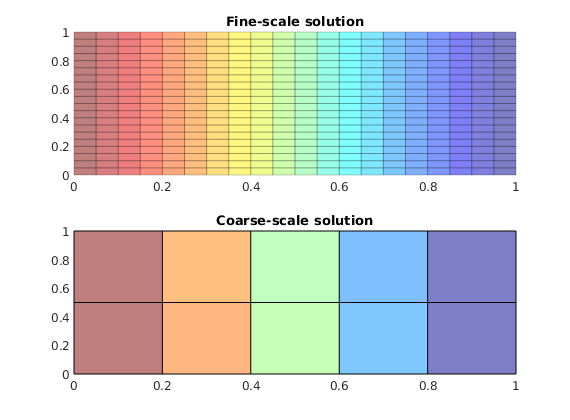
\includegraphics[width=\textwidth]{img/coarsegrid-1.png}
    \caption{Difference between Coarse and Fine Grid.}
\end{figure}

\noindent
But to understand frequency, we have to look at the problem from a one-dimensional point of view, looking at frequencies.
\begin{itemize}
    \item \textbf{Fine Grid} has a high resolution, then many closely spaced points.
    \begin{center}
        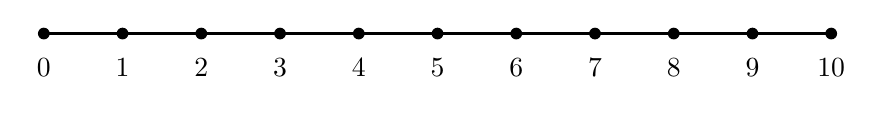
\begin{tikzpicture}
            \def\n{10}
            \foreach \i in {0,...,\n} {
                \node[circle, fill=black, inner sep=1.5pt] at (\i,0) {};
                \node[below] at (\i,-0.2) {\i};
                \ifnum\i>0
                    \draw[thick] (\i-1,0) -- (\i,0);
                \fi
            }
        \end{tikzpicture}
    \end{center}

    \item \textbf{Coarse Grid} has a lower resolution, then fewer points spaced farther apart.
    \begin{center}
        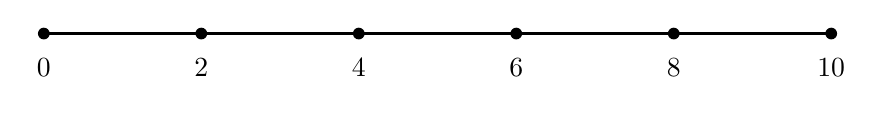
\begin{tikzpicture}
            \foreach \i/\label in {0/0, 1/2, 2/4, 3/6, 4/8, 5/10} {
                \node[circle, fill=black, inner sep=1.5pt] at (\i*2,0) {};
                \node[below] at (\i*2,-0.2) {\label};
                \ifnum\i>0
                    \draw[thick] (\i*2-2,0) -- (\i*2,0);
                \fi
            }
        \end{tikzpicture}
    \end{center}
\end{itemize}

\newpage

\noindent
As we \textbf{move from the fine grid to the coarse grid, the mode becomes more oscillatory because the same error pattern spans fewer points, increasing its apparent frequency}. The term \dquotes{mode} refers to the different error patterns or components in the solution. See the following illustration for a 100\% understanding.

\highspace
Consider a wave function on the fine grid $w_{j} = \sin\left(\dfrac{j \pi}{n+1} i \right)$ (where $j$ determines the frequency, $n$ is the number of points, and $i$ is the index of the grid point), its 1D representation, and the signal:
\begin{center}
    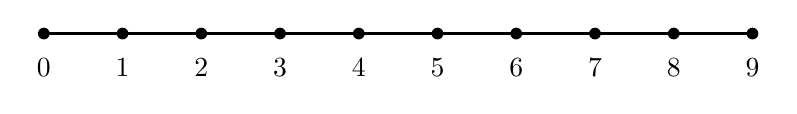
\begin{tikzpicture}
        \def\n{9}
        \foreach \i in {0,...,\n} {
            \node[circle, fill=black, inner sep=1.5pt] at (\i,0) {};
            \node[below] at (\i,-0.2) {\i};
            \ifnum\i>0
                \draw[thick] (\i-1,0) -- (\i,0);
            \fi
        }
    \end{tikzpicture}
\end{center}
\begin{center}
    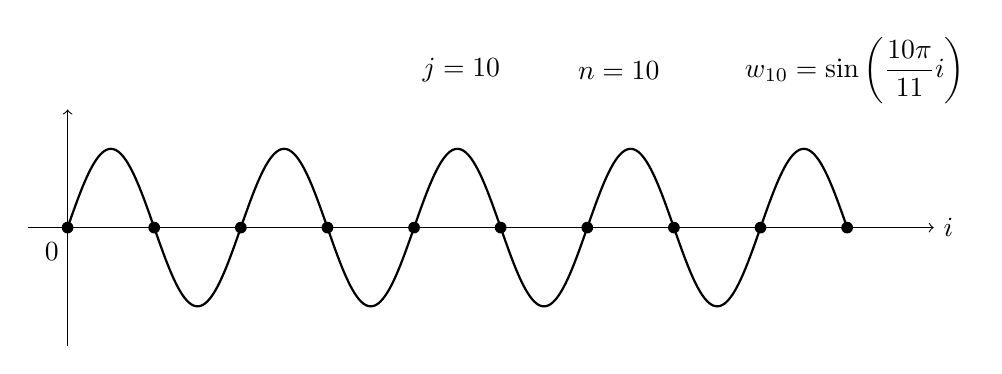
\begin{tikzpicture}
        \draw[->] (-0.5,0) -- (11,0) node[right] {$i$};
        \draw[->] (0,-1.5) -- (0,1.5);
        \node at (-0.2, -0.3) {$0$};

        \draw[thick] plot[domain=0:9.9,samples=1000] (\x,{sin(deg(10*\x*pi/11))});
        
        \foreach \k in {0, 1.1, 2.2, 3.3, 4.4, 5.5, 6.6, 7.7, 8.8, 9.9} {
            \node[circle, fill=black, inner sep=1.5pt] at (\k,0) {};
        }

        \node at (10,2) {$w_{10} = \sin\left(\dfrac{10 \pi}{11} i \right)$};
        \node at (7,2) {$n = 10$};
        \node at (5,2) {$j = 10$};
    \end{tikzpicture}
\end{center}

\noindent
If we pass from the Fine Grid to Coarse Grid reducing the number of points, for example from 10 to 6, we obtain an increase of the oscillatory and also the same error pattern is repeated several times:
\begin{center}
    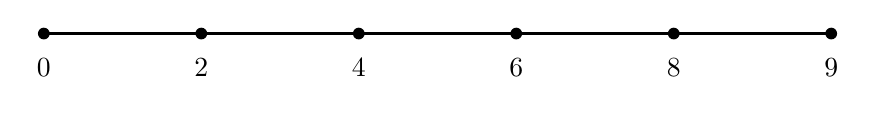
\begin{tikzpicture}
        \foreach \i/\label in {0/0, 1/2, 2/4, 3/6, 4/8, 5/9} {
            \node[circle, fill=black, inner sep=1.5pt] at (\i*2,0) {};
            \node[below] at (\i*2,-0.2) {\label};
            \ifnum\i>0
                \draw[thick] (\i*2-2,0) -- (\i*2,0);
            \fi
        }
    \end{tikzpicture}
\end{center}
\begin{center}
    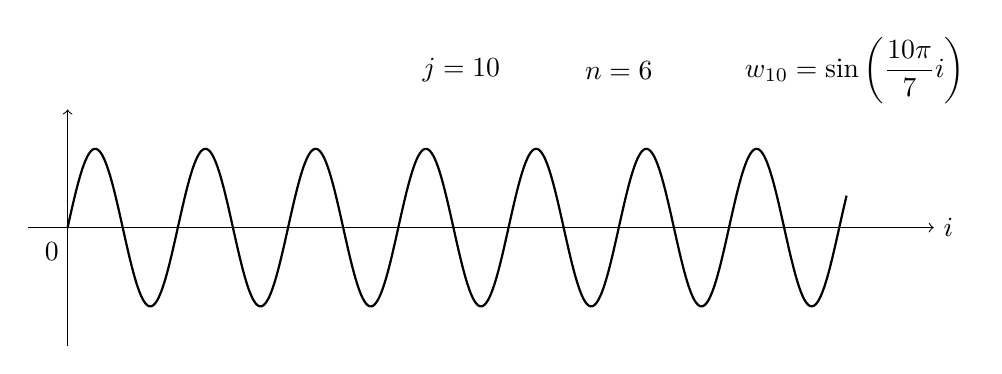
\begin{tikzpicture}
        \draw[->] (-0.5,0) -- (11,0) node[right] {$i$};
        \draw[->] (0,-1.5) -- (0,1.5);
        \node at (-0.2, -0.3) {$0$};

        \draw[thick] plot[domain=0:9.9,samples=1000] (\x,{sin(deg(10*\x*pi/7))});

        \node at (10,2) {$w_{10} = \sin\left(\dfrac{10 \pi}{7} i \right)$};
        \node at (7,2) {$n = 6$};
        \node at (5,2) {$j = 10$};
    \end{tikzpicture}
\end{center}
\newpage
\begin{center}
    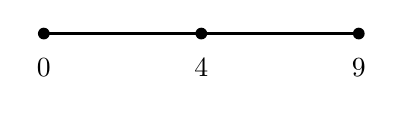
\begin{tikzpicture}
        \foreach \i/\label in {0/0, 1/4, 2/9} {
            \node[circle, fill=black, inner sep=1.5pt] at (\i*2,0) {};
            \node[below] at (\i*2,-0.2) {\label};
            \ifnum\i>0
                \draw[thick] (\i*2-2,0) -- (\i*2,0);
            \fi
        }
    \end{tikzpicture}
\end{center}
\begin{center}
    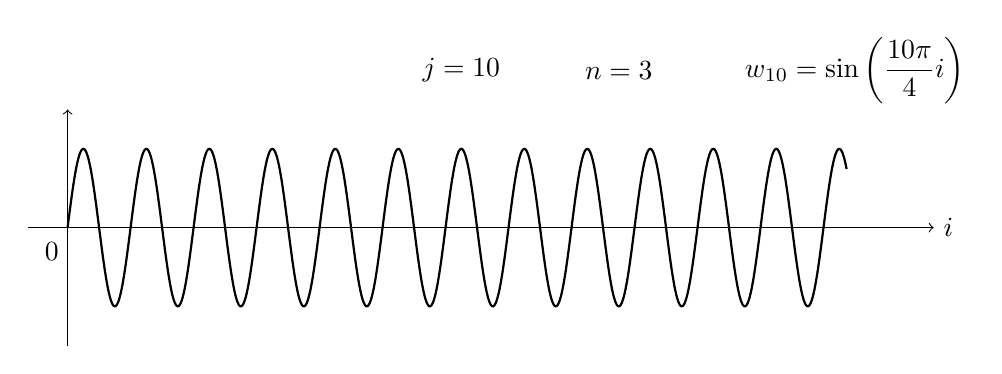
\begin{tikzpicture}
        \draw[->] (-0.5,0) -- (11,0) node[right] {$i$};
        \draw[->] (0,-1.5) -- (0,1.5);
        \node at (-0.2, -0.3) {$0$};

        \draw[thick] plot[domain=0:9.9,samples=1000] (\x,{sin(deg(10*\x*pi/4))});

        \node at (10,2) {$w_{10} = \sin\left(\dfrac{10 \pi}{4} i \right)$};
        \node at (7,2) {$n = 3$};
        \node at (5,2) {$j = 10$};
    \end{tikzpicture}
\end{center}

\noindent
Obviously, \textbf{smooth modes on a Fine Grid will look less smooth on a Coarse Grid}.
    \subsubsection{Correction}\label{subsubsection: Correction}
    \subsubsection{Interpolation Operator}\label{subsubsection: Interpolation Operator}

\textbf{\underline{Purpose}}. The Interpolation Operator transfers corrections from the coarse grid back to the fine grid, refining the fine grid solution with broader adjustments. In other words, it is a powerful operator for \textbf{mapping values from a coarse grid} $\mathcal{F}_{2h}$ \textbf{to a fine grid} $\mathcal{F}_{h}$. This process is essential to transfer the error corrections or residuals from a coarse grid back to a fine grid, thereby increasing the accuracy of the solution.

\highspace
Mathematically, the interpolation operator is a linear operator and it is \textbf{denoted} as a matrix $I^{h}_{2h}$:
\begin{equation}
    \begin{array}{rcl}
        I^{h}_{2h}: \mathcal{F}_{2h} & \longrightarrow & \mathcal{F}_{h} \\ [.5em]
        \mathbb{R}^{n} & \longrightarrow & \mathbb{R}^{m}
    \end{array}
\end{equation}
And it is multiplied by the coarse grid $\mathbf{v}_{2h}$ to get the fine grid with the interpolated values $\mathbf{v}_{h}$:
\begin{equation}
    I^{h}_{2h} \mathbf{v}_{2h} = \mathbf{v}_{h}
\end{equation}
It isn't a simply multiplication, because each position of the fine grid is given by:
\begin{equation*}
    \mathbf{v}_{h,i} = \begin{cases}
        \mathbf{v}_{2h,i} & \text{if the node } i \text{ is common node of both } \mathcal{F}_{h} \text{ and } \mathcal{F}_{2h} \vspace{.8em}\\
        \dfrac{
            \mathbf{v}_{2h,i}^{+} + \mathbf{v}_{2h,i}^{-}
        }{2} & \text{if the node } i \text{ in } \mathcal{F}_{h} \text{ is not a node in } \mathcal{F}_{2h}
    \end{cases}
\end{equation*}
Perhaps this discussion is easier to understand graphically. As we can see, for nodes that exist only in the fine grid and not in the coarse grid, the value is interpolated as the average of the neighboring coarse grid nodes.
\begin{figure}[!htp]
    \centering
    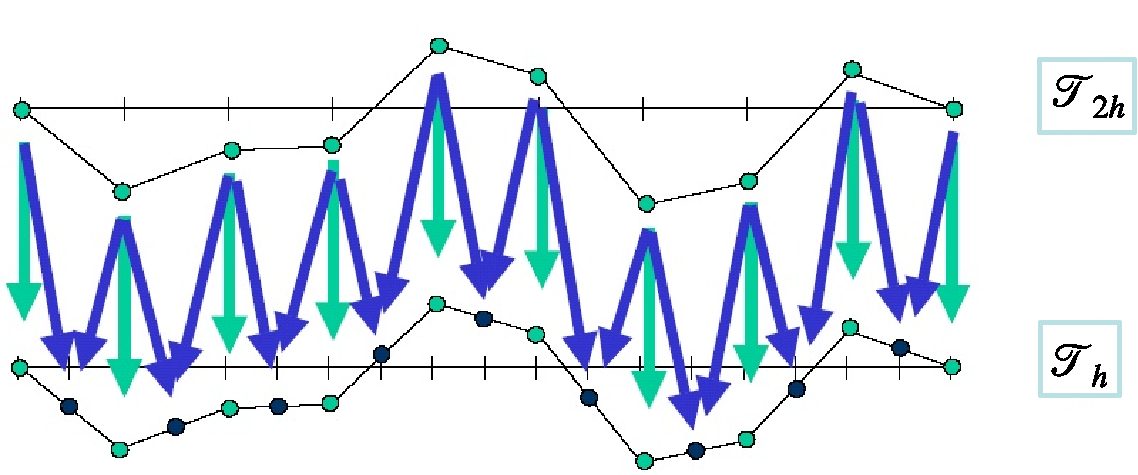
\includegraphics[width=.8\textwidth]{img/interpolation-operator-1.pdf}
\end{figure}

\newpage

\begin{flushleft}
    \textcolor{Green3}{\faIcon{balance-scale} \textbf{Smooth vs Oscillatory errors}}
\end{flushleft}
To fully understand the MG method, it is important to understand when to use it. The interpolation operator highlights when and why the method can be effective or ineffective. \textbf{If the exact error on the fine grid} $\mathcal{F}_{h}$ is:
\begin{itemize}
    \item[\textcolor{Green3}{\faIcon{check-circle}}] \textcolor{Green3}{\textbf{Smooth}}: an interpolation of the coarse grid error $\mathbf{e}_{2h}$ should give a \textbf{good representation} of the exact error.
    
    The smooth errors are errors that change gradually over the grid. So if we interpolate a smooth error from a coarse grid to a fine grid (using the interpolation operator), the interpolation will be accurate. This is because the changes in the error are well captured by the averaging, so that the interpolated fine grid values are very similar to the original smooth error. See the Figure \ref{fig: smooth error} to see why this is a good representation of the exact error.
    
    \begin{figure}[!htp]
    	\centering
    	\resizebox{.9\textwidth}{!}{%% Creator: Matplotlib, PGF backend
%%
%% To include the figure in your LaTeX document, write
%%   \input{<filename>.pgf}
%%
%% Make sure the required packages are loaded in your preamble
%%   \usepackage{pgf}
%%
%% Also ensure that all the required font packages are loaded; for instance,
%% the lmodern package is sometimes necessary when using math font.
%%   \usepackage{lmodern}
%%
%% Figures using additional raster images can only be included by \input if
%% they are in the same directory as the main LaTeX file. For loading figures
%% from other directories you can use the `import` package
%%   \usepackage{import}
%%
%% and then include the figures with
%%   \import{<path to file>}{<filename>.pgf}
%%
%% Matplotlib used the following preamble
%%   \def\mathdefault#1{#1}
%%   \everymath=\expandafter{\the\everymath\displaystyle}
%%   
%%   \ifdefined\pdftexversion\else  % non-pdftex case.
%%     \usepackage{fontspec}
%%     \setmainfont{DejaVuSerif.ttf}[Path=\detokenize{/home/andrevale69/.virtualenvs/test/lib/python3.12/site-packages/matplotlib/mpl-data/fonts/ttf/}]
%%     \setsansfont{DejaVuSans.ttf}[Path=\detokenize{/home/andrevale69/.virtualenvs/test/lib/python3.12/site-packages/matplotlib/mpl-data/fonts/ttf/}]
%%     \setmonofont{DejaVuSansMono.ttf}[Path=\detokenize{/home/andrevale69/.virtualenvs/test/lib/python3.12/site-packages/matplotlib/mpl-data/fonts/ttf/}]
%%   \fi
%%   \makeatletter\@ifpackageloaded{underscore}{}{\usepackage[strings]{underscore}}\makeatother
%%
\begingroup%
\makeatletter%
\begin{pgfpicture}%
\pgfpathrectangle{\pgfpointorigin}{\pgfqpoint{6.000000in}{6.000000in}}%
\pgfusepath{use as bounding box, clip}%
\begin{pgfscope}%
\pgfsetbuttcap%
\pgfsetmiterjoin%
\definecolor{currentfill}{rgb}{1.000000,1.000000,1.000000}%
\pgfsetfillcolor{currentfill}%
\pgfsetlinewidth{0.000000pt}%
\definecolor{currentstroke}{rgb}{1.000000,1.000000,1.000000}%
\pgfsetstrokecolor{currentstroke}%
\pgfsetdash{}{0pt}%
\pgfpathmoveto{\pgfqpoint{0.000000in}{0.000000in}}%
\pgfpathlineto{\pgfqpoint{6.000000in}{0.000000in}}%
\pgfpathlineto{\pgfqpoint{6.000000in}{6.000000in}}%
\pgfpathlineto{\pgfqpoint{0.000000in}{6.000000in}}%
\pgfpathlineto{\pgfqpoint{0.000000in}{0.000000in}}%
\pgfpathclose%
\pgfusepath{fill}%
\end{pgfscope}%
\begin{pgfscope}%
\pgfsetbuttcap%
\pgfsetmiterjoin%
\definecolor{currentfill}{rgb}{1.000000,1.000000,1.000000}%
\pgfsetfillcolor{currentfill}%
\pgfsetlinewidth{0.000000pt}%
\definecolor{currentstroke}{rgb}{0.000000,0.000000,0.000000}%
\pgfsetstrokecolor{currentstroke}%
\pgfsetstrokeopacity{0.000000}%
\pgfsetdash{}{0pt}%
\pgfpathmoveto{\pgfqpoint{0.670972in}{1.235556in}}%
\pgfpathlineto{\pgfqpoint{5.850000in}{1.235556in}}%
\pgfpathlineto{\pgfqpoint{5.850000in}{5.626667in}}%
\pgfpathlineto{\pgfqpoint{0.670972in}{5.626667in}}%
\pgfpathlineto{\pgfqpoint{0.670972in}{1.235556in}}%
\pgfpathclose%
\pgfusepath{fill}%
\end{pgfscope}%
\begin{pgfscope}%
\pgfsetbuttcap%
\pgfsetroundjoin%
\definecolor{currentfill}{rgb}{0.000000,0.000000,0.000000}%
\pgfsetfillcolor{currentfill}%
\pgfsetlinewidth{0.803000pt}%
\definecolor{currentstroke}{rgb}{0.000000,0.000000,0.000000}%
\pgfsetstrokecolor{currentstroke}%
\pgfsetdash{}{0pt}%
\pgfsys@defobject{currentmarker}{\pgfqpoint{0.000000in}{-0.048611in}}{\pgfqpoint{0.000000in}{0.000000in}}{%
\pgfpathmoveto{\pgfqpoint{0.000000in}{0.000000in}}%
\pgfpathlineto{\pgfqpoint{0.000000in}{-0.048611in}}%
\pgfusepath{stroke,fill}%
}%
\begin{pgfscope}%
\pgfsys@transformshift{0.906383in}{1.235556in}%
\pgfsys@useobject{currentmarker}{}%
\end{pgfscope}%
\end{pgfscope}%
\begin{pgfscope}%
\definecolor{textcolor}{rgb}{0.000000,0.000000,0.000000}%
\pgfsetstrokecolor{textcolor}%
\pgfsetfillcolor{textcolor}%
\pgftext[x=0.906383in,y=1.138333in,,top]{\color{textcolor}{\sffamily\fontsize{10.000000}{12.000000}\selectfont\catcode`\^=\active\def^{\ifmmode\sp\else\^{}\fi}\catcode`\%=\active\def%{\%}0}}%
\end{pgfscope}%
\begin{pgfscope}%
\pgfsetbuttcap%
\pgfsetroundjoin%
\definecolor{currentfill}{rgb}{0.000000,0.000000,0.000000}%
\pgfsetfillcolor{currentfill}%
\pgfsetlinewidth{0.803000pt}%
\definecolor{currentstroke}{rgb}{0.000000,0.000000,0.000000}%
\pgfsetstrokecolor{currentstroke}%
\pgfsetdash{}{0pt}%
\pgfsys@defobject{currentmarker}{\pgfqpoint{0.000000in}{-0.048611in}}{\pgfqpoint{0.000000in}{0.000000in}}{%
\pgfpathmoveto{\pgfqpoint{0.000000in}{0.000000in}}%
\pgfpathlineto{\pgfqpoint{0.000000in}{-0.048611in}}%
\pgfusepath{stroke,fill}%
}%
\begin{pgfscope}%
\pgfsys@transformshift{1.848024in}{1.235556in}%
\pgfsys@useobject{currentmarker}{}%
\end{pgfscope}%
\end{pgfscope}%
\begin{pgfscope}%
\definecolor{textcolor}{rgb}{0.000000,0.000000,0.000000}%
\pgfsetstrokecolor{textcolor}%
\pgfsetfillcolor{textcolor}%
\pgftext[x=1.848024in,y=1.138333in,,top]{\color{textcolor}{\sffamily\fontsize{10.000000}{12.000000}\selectfont\catcode`\^=\active\def^{\ifmmode\sp\else\^{}\fi}\catcode`\%=\active\def%{\%}2}}%
\end{pgfscope}%
\begin{pgfscope}%
\pgfsetbuttcap%
\pgfsetroundjoin%
\definecolor{currentfill}{rgb}{0.000000,0.000000,0.000000}%
\pgfsetfillcolor{currentfill}%
\pgfsetlinewidth{0.803000pt}%
\definecolor{currentstroke}{rgb}{0.000000,0.000000,0.000000}%
\pgfsetstrokecolor{currentstroke}%
\pgfsetdash{}{0pt}%
\pgfsys@defobject{currentmarker}{\pgfqpoint{0.000000in}{-0.048611in}}{\pgfqpoint{0.000000in}{0.000000in}}{%
\pgfpathmoveto{\pgfqpoint{0.000000in}{0.000000in}}%
\pgfpathlineto{\pgfqpoint{0.000000in}{-0.048611in}}%
\pgfusepath{stroke,fill}%
}%
\begin{pgfscope}%
\pgfsys@transformshift{2.789665in}{1.235556in}%
\pgfsys@useobject{currentmarker}{}%
\end{pgfscope}%
\end{pgfscope}%
\begin{pgfscope}%
\definecolor{textcolor}{rgb}{0.000000,0.000000,0.000000}%
\pgfsetstrokecolor{textcolor}%
\pgfsetfillcolor{textcolor}%
\pgftext[x=2.789665in,y=1.138333in,,top]{\color{textcolor}{\sffamily\fontsize{10.000000}{12.000000}\selectfont\catcode`\^=\active\def^{\ifmmode\sp\else\^{}\fi}\catcode`\%=\active\def%{\%}4}}%
\end{pgfscope}%
\begin{pgfscope}%
\pgfsetbuttcap%
\pgfsetroundjoin%
\definecolor{currentfill}{rgb}{0.000000,0.000000,0.000000}%
\pgfsetfillcolor{currentfill}%
\pgfsetlinewidth{0.803000pt}%
\definecolor{currentstroke}{rgb}{0.000000,0.000000,0.000000}%
\pgfsetstrokecolor{currentstroke}%
\pgfsetdash{}{0pt}%
\pgfsys@defobject{currentmarker}{\pgfqpoint{0.000000in}{-0.048611in}}{\pgfqpoint{0.000000in}{0.000000in}}{%
\pgfpathmoveto{\pgfqpoint{0.000000in}{0.000000in}}%
\pgfpathlineto{\pgfqpoint{0.000000in}{-0.048611in}}%
\pgfusepath{stroke,fill}%
}%
\begin{pgfscope}%
\pgfsys@transformshift{3.731307in}{1.235556in}%
\pgfsys@useobject{currentmarker}{}%
\end{pgfscope}%
\end{pgfscope}%
\begin{pgfscope}%
\definecolor{textcolor}{rgb}{0.000000,0.000000,0.000000}%
\pgfsetstrokecolor{textcolor}%
\pgfsetfillcolor{textcolor}%
\pgftext[x=3.731307in,y=1.138333in,,top]{\color{textcolor}{\sffamily\fontsize{10.000000}{12.000000}\selectfont\catcode`\^=\active\def^{\ifmmode\sp\else\^{}\fi}\catcode`\%=\active\def%{\%}6}}%
\end{pgfscope}%
\begin{pgfscope}%
\pgfsetbuttcap%
\pgfsetroundjoin%
\definecolor{currentfill}{rgb}{0.000000,0.000000,0.000000}%
\pgfsetfillcolor{currentfill}%
\pgfsetlinewidth{0.803000pt}%
\definecolor{currentstroke}{rgb}{0.000000,0.000000,0.000000}%
\pgfsetstrokecolor{currentstroke}%
\pgfsetdash{}{0pt}%
\pgfsys@defobject{currentmarker}{\pgfqpoint{0.000000in}{-0.048611in}}{\pgfqpoint{0.000000in}{0.000000in}}{%
\pgfpathmoveto{\pgfqpoint{0.000000in}{0.000000in}}%
\pgfpathlineto{\pgfqpoint{0.000000in}{-0.048611in}}%
\pgfusepath{stroke,fill}%
}%
\begin{pgfscope}%
\pgfsys@transformshift{4.672948in}{1.235556in}%
\pgfsys@useobject{currentmarker}{}%
\end{pgfscope}%
\end{pgfscope}%
\begin{pgfscope}%
\definecolor{textcolor}{rgb}{0.000000,0.000000,0.000000}%
\pgfsetstrokecolor{textcolor}%
\pgfsetfillcolor{textcolor}%
\pgftext[x=4.672948in,y=1.138333in,,top]{\color{textcolor}{\sffamily\fontsize{10.000000}{12.000000}\selectfont\catcode`\^=\active\def^{\ifmmode\sp\else\^{}\fi}\catcode`\%=\active\def%{\%}8}}%
\end{pgfscope}%
\begin{pgfscope}%
\pgfsetbuttcap%
\pgfsetroundjoin%
\definecolor{currentfill}{rgb}{0.000000,0.000000,0.000000}%
\pgfsetfillcolor{currentfill}%
\pgfsetlinewidth{0.803000pt}%
\definecolor{currentstroke}{rgb}{0.000000,0.000000,0.000000}%
\pgfsetstrokecolor{currentstroke}%
\pgfsetdash{}{0pt}%
\pgfsys@defobject{currentmarker}{\pgfqpoint{0.000000in}{-0.048611in}}{\pgfqpoint{0.000000in}{0.000000in}}{%
\pgfpathmoveto{\pgfqpoint{0.000000in}{0.000000in}}%
\pgfpathlineto{\pgfqpoint{0.000000in}{-0.048611in}}%
\pgfusepath{stroke,fill}%
}%
\begin{pgfscope}%
\pgfsys@transformshift{5.614590in}{1.235556in}%
\pgfsys@useobject{currentmarker}{}%
\end{pgfscope}%
\end{pgfscope}%
\begin{pgfscope}%
\definecolor{textcolor}{rgb}{0.000000,0.000000,0.000000}%
\pgfsetstrokecolor{textcolor}%
\pgfsetfillcolor{textcolor}%
\pgftext[x=5.614590in,y=1.138333in,,top]{\color{textcolor}{\sffamily\fontsize{10.000000}{12.000000}\selectfont\catcode`\^=\active\def^{\ifmmode\sp\else\^{}\fi}\catcode`\%=\active\def%{\%}10}}%
\end{pgfscope}%
\begin{pgfscope}%
\pgfsetbuttcap%
\pgfsetroundjoin%
\definecolor{currentfill}{rgb}{0.000000,0.000000,0.000000}%
\pgfsetfillcolor{currentfill}%
\pgfsetlinewidth{0.803000pt}%
\definecolor{currentstroke}{rgb}{0.000000,0.000000,0.000000}%
\pgfsetstrokecolor{currentstroke}%
\pgfsetdash{}{0pt}%
\pgfsys@defobject{currentmarker}{\pgfqpoint{-0.048611in}{0.000000in}}{\pgfqpoint{-0.000000in}{0.000000in}}{%
\pgfpathmoveto{\pgfqpoint{-0.000000in}{0.000000in}}%
\pgfpathlineto{\pgfqpoint{-0.048611in}{0.000000in}}%
\pgfusepath{stroke,fill}%
}%
\begin{pgfscope}%
\pgfsys@transformshift{0.670972in}{1.434809in}%
\pgfsys@useobject{currentmarker}{}%
\end{pgfscope}%
\end{pgfscope}%
\begin{pgfscope}%
\definecolor{textcolor}{rgb}{0.000000,0.000000,0.000000}%
\pgfsetstrokecolor{textcolor}%
\pgfsetfillcolor{textcolor}%
\pgftext[x=0.156480in, y=1.382048in, left, base]{\color{textcolor}{\sffamily\fontsize{10.000000}{12.000000}\selectfont\catcode`\^=\active\def^{\ifmmode\sp\else\^{}\fi}\catcode`\%=\active\def%{\%}\ensuremath{-}1.00}}%
\end{pgfscope}%
\begin{pgfscope}%
\pgfsetbuttcap%
\pgfsetroundjoin%
\definecolor{currentfill}{rgb}{0.000000,0.000000,0.000000}%
\pgfsetfillcolor{currentfill}%
\pgfsetlinewidth{0.803000pt}%
\definecolor{currentstroke}{rgb}{0.000000,0.000000,0.000000}%
\pgfsetstrokecolor{currentstroke}%
\pgfsetdash{}{0pt}%
\pgfsys@defobject{currentmarker}{\pgfqpoint{-0.048611in}{0.000000in}}{\pgfqpoint{-0.000000in}{0.000000in}}{%
\pgfpathmoveto{\pgfqpoint{-0.000000in}{0.000000in}}%
\pgfpathlineto{\pgfqpoint{-0.048611in}{0.000000in}}%
\pgfusepath{stroke,fill}%
}%
\begin{pgfscope}%
\pgfsys@transformshift{0.670972in}{1.934320in}%
\pgfsys@useobject{currentmarker}{}%
\end{pgfscope}%
\end{pgfscope}%
\begin{pgfscope}%
\definecolor{textcolor}{rgb}{0.000000,0.000000,0.000000}%
\pgfsetstrokecolor{textcolor}%
\pgfsetfillcolor{textcolor}%
\pgftext[x=0.156480in, y=1.881558in, left, base]{\color{textcolor}{\sffamily\fontsize{10.000000}{12.000000}\selectfont\catcode`\^=\active\def^{\ifmmode\sp\else\^{}\fi}\catcode`\%=\active\def%{\%}\ensuremath{-}0.75}}%
\end{pgfscope}%
\begin{pgfscope}%
\pgfsetbuttcap%
\pgfsetroundjoin%
\definecolor{currentfill}{rgb}{0.000000,0.000000,0.000000}%
\pgfsetfillcolor{currentfill}%
\pgfsetlinewidth{0.803000pt}%
\definecolor{currentstroke}{rgb}{0.000000,0.000000,0.000000}%
\pgfsetstrokecolor{currentstroke}%
\pgfsetdash{}{0pt}%
\pgfsys@defobject{currentmarker}{\pgfqpoint{-0.048611in}{0.000000in}}{\pgfqpoint{-0.000000in}{0.000000in}}{%
\pgfpathmoveto{\pgfqpoint{-0.000000in}{0.000000in}}%
\pgfpathlineto{\pgfqpoint{-0.048611in}{0.000000in}}%
\pgfusepath{stroke,fill}%
}%
\begin{pgfscope}%
\pgfsys@transformshift{0.670972in}{2.433830in}%
\pgfsys@useobject{currentmarker}{}%
\end{pgfscope}%
\end{pgfscope}%
\begin{pgfscope}%
\definecolor{textcolor}{rgb}{0.000000,0.000000,0.000000}%
\pgfsetstrokecolor{textcolor}%
\pgfsetfillcolor{textcolor}%
\pgftext[x=0.156480in, y=2.381068in, left, base]{\color{textcolor}{\sffamily\fontsize{10.000000}{12.000000}\selectfont\catcode`\^=\active\def^{\ifmmode\sp\else\^{}\fi}\catcode`\%=\active\def%{\%}\ensuremath{-}0.50}}%
\end{pgfscope}%
\begin{pgfscope}%
\pgfsetbuttcap%
\pgfsetroundjoin%
\definecolor{currentfill}{rgb}{0.000000,0.000000,0.000000}%
\pgfsetfillcolor{currentfill}%
\pgfsetlinewidth{0.803000pt}%
\definecolor{currentstroke}{rgb}{0.000000,0.000000,0.000000}%
\pgfsetstrokecolor{currentstroke}%
\pgfsetdash{}{0pt}%
\pgfsys@defobject{currentmarker}{\pgfqpoint{-0.048611in}{0.000000in}}{\pgfqpoint{-0.000000in}{0.000000in}}{%
\pgfpathmoveto{\pgfqpoint{-0.000000in}{0.000000in}}%
\pgfpathlineto{\pgfqpoint{-0.048611in}{0.000000in}}%
\pgfusepath{stroke,fill}%
}%
\begin{pgfscope}%
\pgfsys@transformshift{0.670972in}{2.933340in}%
\pgfsys@useobject{currentmarker}{}%
\end{pgfscope}%
\end{pgfscope}%
\begin{pgfscope}%
\definecolor{textcolor}{rgb}{0.000000,0.000000,0.000000}%
\pgfsetstrokecolor{textcolor}%
\pgfsetfillcolor{textcolor}%
\pgftext[x=0.156480in, y=2.880579in, left, base]{\color{textcolor}{\sffamily\fontsize{10.000000}{12.000000}\selectfont\catcode`\^=\active\def^{\ifmmode\sp\else\^{}\fi}\catcode`\%=\active\def%{\%}\ensuremath{-}0.25}}%
\end{pgfscope}%
\begin{pgfscope}%
\pgfsetbuttcap%
\pgfsetroundjoin%
\definecolor{currentfill}{rgb}{0.000000,0.000000,0.000000}%
\pgfsetfillcolor{currentfill}%
\pgfsetlinewidth{0.803000pt}%
\definecolor{currentstroke}{rgb}{0.000000,0.000000,0.000000}%
\pgfsetstrokecolor{currentstroke}%
\pgfsetdash{}{0pt}%
\pgfsys@defobject{currentmarker}{\pgfqpoint{-0.048611in}{0.000000in}}{\pgfqpoint{-0.000000in}{0.000000in}}{%
\pgfpathmoveto{\pgfqpoint{-0.000000in}{0.000000in}}%
\pgfpathlineto{\pgfqpoint{-0.048611in}{0.000000in}}%
\pgfusepath{stroke,fill}%
}%
\begin{pgfscope}%
\pgfsys@transformshift{0.670972in}{3.432851in}%
\pgfsys@useobject{currentmarker}{}%
\end{pgfscope}%
\end{pgfscope}%
\begin{pgfscope}%
\definecolor{textcolor}{rgb}{0.000000,0.000000,0.000000}%
\pgfsetstrokecolor{textcolor}%
\pgfsetfillcolor{textcolor}%
\pgftext[x=0.264505in, y=3.380089in, left, base]{\color{textcolor}{\sffamily\fontsize{10.000000}{12.000000}\selectfont\catcode`\^=\active\def^{\ifmmode\sp\else\^{}\fi}\catcode`\%=\active\def%{\%}0.00}}%
\end{pgfscope}%
\begin{pgfscope}%
\pgfsetbuttcap%
\pgfsetroundjoin%
\definecolor{currentfill}{rgb}{0.000000,0.000000,0.000000}%
\pgfsetfillcolor{currentfill}%
\pgfsetlinewidth{0.803000pt}%
\definecolor{currentstroke}{rgb}{0.000000,0.000000,0.000000}%
\pgfsetstrokecolor{currentstroke}%
\pgfsetdash{}{0pt}%
\pgfsys@defobject{currentmarker}{\pgfqpoint{-0.048611in}{0.000000in}}{\pgfqpoint{-0.000000in}{0.000000in}}{%
\pgfpathmoveto{\pgfqpoint{-0.000000in}{0.000000in}}%
\pgfpathlineto{\pgfqpoint{-0.048611in}{0.000000in}}%
\pgfusepath{stroke,fill}%
}%
\begin{pgfscope}%
\pgfsys@transformshift{0.670972in}{3.932361in}%
\pgfsys@useobject{currentmarker}{}%
\end{pgfscope}%
\end{pgfscope}%
\begin{pgfscope}%
\definecolor{textcolor}{rgb}{0.000000,0.000000,0.000000}%
\pgfsetstrokecolor{textcolor}%
\pgfsetfillcolor{textcolor}%
\pgftext[x=0.264505in, y=3.879599in, left, base]{\color{textcolor}{\sffamily\fontsize{10.000000}{12.000000}\selectfont\catcode`\^=\active\def^{\ifmmode\sp\else\^{}\fi}\catcode`\%=\active\def%{\%}0.25}}%
\end{pgfscope}%
\begin{pgfscope}%
\pgfsetbuttcap%
\pgfsetroundjoin%
\definecolor{currentfill}{rgb}{0.000000,0.000000,0.000000}%
\pgfsetfillcolor{currentfill}%
\pgfsetlinewidth{0.803000pt}%
\definecolor{currentstroke}{rgb}{0.000000,0.000000,0.000000}%
\pgfsetstrokecolor{currentstroke}%
\pgfsetdash{}{0pt}%
\pgfsys@defobject{currentmarker}{\pgfqpoint{-0.048611in}{0.000000in}}{\pgfqpoint{-0.000000in}{0.000000in}}{%
\pgfpathmoveto{\pgfqpoint{-0.000000in}{0.000000in}}%
\pgfpathlineto{\pgfqpoint{-0.048611in}{0.000000in}}%
\pgfusepath{stroke,fill}%
}%
\begin{pgfscope}%
\pgfsys@transformshift{0.670972in}{4.431871in}%
\pgfsys@useobject{currentmarker}{}%
\end{pgfscope}%
\end{pgfscope}%
\begin{pgfscope}%
\definecolor{textcolor}{rgb}{0.000000,0.000000,0.000000}%
\pgfsetstrokecolor{textcolor}%
\pgfsetfillcolor{textcolor}%
\pgftext[x=0.264505in, y=4.379110in, left, base]{\color{textcolor}{\sffamily\fontsize{10.000000}{12.000000}\selectfont\catcode`\^=\active\def^{\ifmmode\sp\else\^{}\fi}\catcode`\%=\active\def%{\%}0.50}}%
\end{pgfscope}%
\begin{pgfscope}%
\pgfsetbuttcap%
\pgfsetroundjoin%
\definecolor{currentfill}{rgb}{0.000000,0.000000,0.000000}%
\pgfsetfillcolor{currentfill}%
\pgfsetlinewidth{0.803000pt}%
\definecolor{currentstroke}{rgb}{0.000000,0.000000,0.000000}%
\pgfsetstrokecolor{currentstroke}%
\pgfsetdash{}{0pt}%
\pgfsys@defobject{currentmarker}{\pgfqpoint{-0.048611in}{0.000000in}}{\pgfqpoint{-0.000000in}{0.000000in}}{%
\pgfpathmoveto{\pgfqpoint{-0.000000in}{0.000000in}}%
\pgfpathlineto{\pgfqpoint{-0.048611in}{0.000000in}}%
\pgfusepath{stroke,fill}%
}%
\begin{pgfscope}%
\pgfsys@transformshift{0.670972in}{4.931382in}%
\pgfsys@useobject{currentmarker}{}%
\end{pgfscope}%
\end{pgfscope}%
\begin{pgfscope}%
\definecolor{textcolor}{rgb}{0.000000,0.000000,0.000000}%
\pgfsetstrokecolor{textcolor}%
\pgfsetfillcolor{textcolor}%
\pgftext[x=0.264505in, y=4.878620in, left, base]{\color{textcolor}{\sffamily\fontsize{10.000000}{12.000000}\selectfont\catcode`\^=\active\def^{\ifmmode\sp\else\^{}\fi}\catcode`\%=\active\def%{\%}0.75}}%
\end{pgfscope}%
\begin{pgfscope}%
\pgfsetbuttcap%
\pgfsetroundjoin%
\definecolor{currentfill}{rgb}{0.000000,0.000000,0.000000}%
\pgfsetfillcolor{currentfill}%
\pgfsetlinewidth{0.803000pt}%
\definecolor{currentstroke}{rgb}{0.000000,0.000000,0.000000}%
\pgfsetstrokecolor{currentstroke}%
\pgfsetdash{}{0pt}%
\pgfsys@defobject{currentmarker}{\pgfqpoint{-0.048611in}{0.000000in}}{\pgfqpoint{-0.000000in}{0.000000in}}{%
\pgfpathmoveto{\pgfqpoint{-0.000000in}{0.000000in}}%
\pgfpathlineto{\pgfqpoint{-0.048611in}{0.000000in}}%
\pgfusepath{stroke,fill}%
}%
\begin{pgfscope}%
\pgfsys@transformshift{0.670972in}{5.430892in}%
\pgfsys@useobject{currentmarker}{}%
\end{pgfscope}%
\end{pgfscope}%
\begin{pgfscope}%
\definecolor{textcolor}{rgb}{0.000000,0.000000,0.000000}%
\pgfsetstrokecolor{textcolor}%
\pgfsetfillcolor{textcolor}%
\pgftext[x=0.264505in, y=5.378130in, left, base]{\color{textcolor}{\sffamily\fontsize{10.000000}{12.000000}\selectfont\catcode`\^=\active\def^{\ifmmode\sp\else\^{}\fi}\catcode`\%=\active\def%{\%}1.00}}%
\end{pgfscope}%
\begin{pgfscope}%
\pgfpathrectangle{\pgfqpoint{0.670972in}{1.235556in}}{\pgfqpoint{5.179028in}{4.391111in}}%
\pgfusepath{clip}%
\pgfsetrectcap%
\pgfsetroundjoin%
\pgfsetlinewidth{1.505625pt}%
\definecolor{currentstroke}{rgb}{0.121569,0.466667,0.705882}%
\pgfsetstrokecolor{currentstroke}%
\pgfsetdash{}{0pt}%
\pgfpathmoveto{\pgfqpoint{0.906383in}{3.432851in}}%
\pgfpathlineto{\pgfqpoint{1.848024in}{5.249665in}}%
\pgfpathlineto{\pgfqpoint{2.789665in}{1.920728in}}%
\pgfpathlineto{\pgfqpoint{3.731307in}{2.874567in}}%
\pgfpathlineto{\pgfqpoint{4.672948in}{5.409629in}}%
\pgfpathlineto{\pgfqpoint{5.614590in}{2.345874in}}%
\pgfusepath{stroke}%
\end{pgfscope}%
\begin{pgfscope}%
\pgfpathrectangle{\pgfqpoint{0.670972in}{1.235556in}}{\pgfqpoint{5.179028in}{4.391111in}}%
\pgfusepath{clip}%
\pgfsetbuttcap%
\pgfsetroundjoin%
\definecolor{currentfill}{rgb}{0.121569,0.466667,0.705882}%
\pgfsetfillcolor{currentfill}%
\pgfsetlinewidth{1.003750pt}%
\definecolor{currentstroke}{rgb}{0.121569,0.466667,0.705882}%
\pgfsetstrokecolor{currentstroke}%
\pgfsetdash{}{0pt}%
\pgfsys@defobject{currentmarker}{\pgfqpoint{-0.041667in}{-0.041667in}}{\pgfqpoint{0.041667in}{0.041667in}}{%
\pgfpathmoveto{\pgfqpoint{0.000000in}{-0.041667in}}%
\pgfpathcurveto{\pgfqpoint{0.011050in}{-0.041667in}}{\pgfqpoint{0.021649in}{-0.037276in}}{\pgfqpoint{0.029463in}{-0.029463in}}%
\pgfpathcurveto{\pgfqpoint{0.037276in}{-0.021649in}}{\pgfqpoint{0.041667in}{-0.011050in}}{\pgfqpoint{0.041667in}{0.000000in}}%
\pgfpathcurveto{\pgfqpoint{0.041667in}{0.011050in}}{\pgfqpoint{0.037276in}{0.021649in}}{\pgfqpoint{0.029463in}{0.029463in}}%
\pgfpathcurveto{\pgfqpoint{0.021649in}{0.037276in}}{\pgfqpoint{0.011050in}{0.041667in}}{\pgfqpoint{0.000000in}{0.041667in}}%
\pgfpathcurveto{\pgfqpoint{-0.011050in}{0.041667in}}{\pgfqpoint{-0.021649in}{0.037276in}}{\pgfqpoint{-0.029463in}{0.029463in}}%
\pgfpathcurveto{\pgfqpoint{-0.037276in}{0.021649in}}{\pgfqpoint{-0.041667in}{0.011050in}}{\pgfqpoint{-0.041667in}{0.000000in}}%
\pgfpathcurveto{\pgfqpoint{-0.041667in}{-0.011050in}}{\pgfqpoint{-0.037276in}{-0.021649in}}{\pgfqpoint{-0.029463in}{-0.029463in}}%
\pgfpathcurveto{\pgfqpoint{-0.021649in}{-0.037276in}}{\pgfqpoint{-0.011050in}{-0.041667in}}{\pgfqpoint{0.000000in}{-0.041667in}}%
\pgfpathlineto{\pgfqpoint{0.000000in}{-0.041667in}}%
\pgfpathclose%
\pgfusepath{stroke,fill}%
}%
\begin{pgfscope}%
\pgfsys@transformshift{0.906383in}{3.432851in}%
\pgfsys@useobject{currentmarker}{}%
\end{pgfscope}%
\begin{pgfscope}%
\pgfsys@transformshift{1.848024in}{5.249665in}%
\pgfsys@useobject{currentmarker}{}%
\end{pgfscope}%
\begin{pgfscope}%
\pgfsys@transformshift{2.789665in}{1.920728in}%
\pgfsys@useobject{currentmarker}{}%
\end{pgfscope}%
\begin{pgfscope}%
\pgfsys@transformshift{3.731307in}{2.874567in}%
\pgfsys@useobject{currentmarker}{}%
\end{pgfscope}%
\begin{pgfscope}%
\pgfsys@transformshift{4.672948in}{5.409629in}%
\pgfsys@useobject{currentmarker}{}%
\end{pgfscope}%
\begin{pgfscope}%
\pgfsys@transformshift{5.614590in}{2.345874in}%
\pgfsys@useobject{currentmarker}{}%
\end{pgfscope}%
\end{pgfscope}%
\begin{pgfscope}%
\pgfpathrectangle{\pgfqpoint{0.670972in}{1.235556in}}{\pgfqpoint{5.179028in}{4.391111in}}%
\pgfusepath{clip}%
\pgfsetrectcap%
\pgfsetroundjoin%
\pgfsetlinewidth{1.505625pt}%
\definecolor{currentstroke}{rgb}{1.000000,0.498039,0.054902}%
\pgfsetstrokecolor{currentstroke}%
\pgfsetdash{}{0pt}%
\pgfpathmoveto{\pgfqpoint{0.906383in}{3.432851in}}%
\pgfpathlineto{\pgfqpoint{1.002468in}{3.837790in}}%
\pgfpathlineto{\pgfqpoint{1.098554in}{4.225921in}}%
\pgfpathlineto{\pgfqpoint{1.194640in}{4.581137in}}%
\pgfpathlineto{\pgfqpoint{1.290726in}{4.888693in}}%
\pgfpathlineto{\pgfqpoint{1.386812in}{5.135824in}}%
\pgfpathlineto{\pgfqpoint{1.482898in}{5.312274in}}%
\pgfpathlineto{\pgfqpoint{1.578984in}{5.410718in}}%
\pgfpathlineto{\pgfqpoint{1.675069in}{5.427071in}}%
\pgfpathlineto{\pgfqpoint{1.771155in}{5.360653in}}%
\pgfpathlineto{\pgfqpoint{1.867241in}{5.214223in}}%
\pgfpathlineto{\pgfqpoint{1.963327in}{4.993856in}}%
\pgfpathlineto{\pgfqpoint{2.059413in}{4.708701in}}%
\pgfpathlineto{\pgfqpoint{2.155499in}{4.370591in}}%
\pgfpathlineto{\pgfqpoint{2.251585in}{3.993560in}}%
\pgfpathlineto{\pgfqpoint{2.347670in}{3.593257in}}%
\pgfpathlineto{\pgfqpoint{2.443756in}{3.186296in}}%
\pgfpathlineto{\pgfqpoint{2.539842in}{2.789569in}}%
\pgfpathlineto{\pgfqpoint{2.635928in}{2.419540in}}%
\pgfpathlineto{\pgfqpoint{2.732014in}{2.091570in}}%
\pgfpathlineto{\pgfqpoint{2.828100in}{1.819269in}}%
\pgfpathlineto{\pgfqpoint{2.924186in}{1.613940in}}%
\pgfpathlineto{\pgfqpoint{3.020271in}{1.484104in}}%
\pgfpathlineto{\pgfqpoint{3.116357in}{1.435152in}}%
\pgfpathlineto{\pgfqpoint{3.212443in}{1.469113in}}%
\pgfpathlineto{\pgfqpoint{3.308529in}{1.584580in}}%
\pgfpathlineto{\pgfqpoint{3.404615in}{1.776759in}}%
\pgfpathlineto{\pgfqpoint{3.500701in}{2.037673in}}%
\pgfpathlineto{\pgfqpoint{3.596787in}{2.356495in}}%
\pgfpathlineto{\pgfqpoint{3.692872in}{2.719991in}}%
\pgfpathlineto{\pgfqpoint{3.788958in}{3.113074in}}%
\pgfpathlineto{\pgfqpoint{3.885044in}{3.519429in}}%
\pgfpathlineto{\pgfqpoint{3.981130in}{3.922191in}}%
\pgfpathlineto{\pgfqpoint{4.077216in}{4.304643in}}%
\pgfpathlineto{\pgfqpoint{4.173302in}{4.650911in}}%
\pgfpathlineto{\pgfqpoint{4.269388in}{4.946624in}}%
\pgfpathlineto{\pgfqpoint{4.365473in}{5.179507in}}%
\pgfpathlineto{\pgfqpoint{4.461559in}{5.339896in}}%
\pgfpathlineto{\pgfqpoint{4.557645in}{5.421132in}}%
\pgfpathlineto{\pgfqpoint{4.653731in}{5.419846in}}%
\pgfpathlineto{\pgfqpoint{4.749817in}{5.336089in}}%
\pgfpathlineto{\pgfqpoint{4.845903in}{5.173338in}}%
\pgfpathlineto{\pgfqpoint{4.941989in}{4.938348in}}%
\pgfpathlineto{\pgfqpoint{5.038074in}{4.640873in}}%
\pgfpathlineto{\pgfqpoint{5.134160in}{4.293259in}}%
\pgfpathlineto{\pgfqpoint{5.230246in}{3.909934in}}%
\pgfpathlineto{\pgfqpoint{5.326332in}{3.506807in}}%
\pgfpathlineto{\pgfqpoint{5.422418in}{3.100611in}}%
\pgfpathlineto{\pgfqpoint{5.518504in}{2.708204in}}%
\pgfpathlineto{\pgfqpoint{5.614590in}{2.345874in}}%
\pgfusepath{stroke}%
\end{pgfscope}%
\begin{pgfscope}%
\pgfpathrectangle{\pgfqpoint{0.670972in}{1.235556in}}{\pgfqpoint{5.179028in}{4.391111in}}%
\pgfusepath{clip}%
\pgfsetbuttcap%
\pgfsetroundjoin%
\definecolor{currentfill}{rgb}{1.000000,0.498039,0.054902}%
\pgfsetfillcolor{currentfill}%
\pgfsetlinewidth{1.003750pt}%
\definecolor{currentstroke}{rgb}{1.000000,0.498039,0.054902}%
\pgfsetstrokecolor{currentstroke}%
\pgfsetdash{}{0pt}%
\pgfsys@defobject{currentmarker}{\pgfqpoint{-0.041667in}{-0.041667in}}{\pgfqpoint{0.041667in}{0.041667in}}{%
\pgfpathmoveto{\pgfqpoint{-0.041667in}{-0.041667in}}%
\pgfpathlineto{\pgfqpoint{0.041667in}{0.041667in}}%
\pgfpathmoveto{\pgfqpoint{-0.041667in}{0.041667in}}%
\pgfpathlineto{\pgfqpoint{0.041667in}{-0.041667in}}%
\pgfusepath{stroke,fill}%
}%
\begin{pgfscope}%
\pgfsys@transformshift{0.906383in}{3.432851in}%
\pgfsys@useobject{currentmarker}{}%
\end{pgfscope}%
\begin{pgfscope}%
\pgfsys@transformshift{1.002468in}{3.837790in}%
\pgfsys@useobject{currentmarker}{}%
\end{pgfscope}%
\begin{pgfscope}%
\pgfsys@transformshift{1.098554in}{4.225921in}%
\pgfsys@useobject{currentmarker}{}%
\end{pgfscope}%
\begin{pgfscope}%
\pgfsys@transformshift{1.194640in}{4.581137in}%
\pgfsys@useobject{currentmarker}{}%
\end{pgfscope}%
\begin{pgfscope}%
\pgfsys@transformshift{1.290726in}{4.888693in}%
\pgfsys@useobject{currentmarker}{}%
\end{pgfscope}%
\begin{pgfscope}%
\pgfsys@transformshift{1.386812in}{5.135824in}%
\pgfsys@useobject{currentmarker}{}%
\end{pgfscope}%
\begin{pgfscope}%
\pgfsys@transformshift{1.482898in}{5.312274in}%
\pgfsys@useobject{currentmarker}{}%
\end{pgfscope}%
\begin{pgfscope}%
\pgfsys@transformshift{1.578984in}{5.410718in}%
\pgfsys@useobject{currentmarker}{}%
\end{pgfscope}%
\begin{pgfscope}%
\pgfsys@transformshift{1.675069in}{5.427071in}%
\pgfsys@useobject{currentmarker}{}%
\end{pgfscope}%
\begin{pgfscope}%
\pgfsys@transformshift{1.771155in}{5.360653in}%
\pgfsys@useobject{currentmarker}{}%
\end{pgfscope}%
\begin{pgfscope}%
\pgfsys@transformshift{1.867241in}{5.214223in}%
\pgfsys@useobject{currentmarker}{}%
\end{pgfscope}%
\begin{pgfscope}%
\pgfsys@transformshift{1.963327in}{4.993856in}%
\pgfsys@useobject{currentmarker}{}%
\end{pgfscope}%
\begin{pgfscope}%
\pgfsys@transformshift{2.059413in}{4.708701in}%
\pgfsys@useobject{currentmarker}{}%
\end{pgfscope}%
\begin{pgfscope}%
\pgfsys@transformshift{2.155499in}{4.370591in}%
\pgfsys@useobject{currentmarker}{}%
\end{pgfscope}%
\begin{pgfscope}%
\pgfsys@transformshift{2.251585in}{3.993560in}%
\pgfsys@useobject{currentmarker}{}%
\end{pgfscope}%
\begin{pgfscope}%
\pgfsys@transformshift{2.347670in}{3.593257in}%
\pgfsys@useobject{currentmarker}{}%
\end{pgfscope}%
\begin{pgfscope}%
\pgfsys@transformshift{2.443756in}{3.186296in}%
\pgfsys@useobject{currentmarker}{}%
\end{pgfscope}%
\begin{pgfscope}%
\pgfsys@transformshift{2.539842in}{2.789569in}%
\pgfsys@useobject{currentmarker}{}%
\end{pgfscope}%
\begin{pgfscope}%
\pgfsys@transformshift{2.635928in}{2.419540in}%
\pgfsys@useobject{currentmarker}{}%
\end{pgfscope}%
\begin{pgfscope}%
\pgfsys@transformshift{2.732014in}{2.091570in}%
\pgfsys@useobject{currentmarker}{}%
\end{pgfscope}%
\begin{pgfscope}%
\pgfsys@transformshift{2.828100in}{1.819269in}%
\pgfsys@useobject{currentmarker}{}%
\end{pgfscope}%
\begin{pgfscope}%
\pgfsys@transformshift{2.924186in}{1.613940in}%
\pgfsys@useobject{currentmarker}{}%
\end{pgfscope}%
\begin{pgfscope}%
\pgfsys@transformshift{3.020271in}{1.484104in}%
\pgfsys@useobject{currentmarker}{}%
\end{pgfscope}%
\begin{pgfscope}%
\pgfsys@transformshift{3.116357in}{1.435152in}%
\pgfsys@useobject{currentmarker}{}%
\end{pgfscope}%
\begin{pgfscope}%
\pgfsys@transformshift{3.212443in}{1.469113in}%
\pgfsys@useobject{currentmarker}{}%
\end{pgfscope}%
\begin{pgfscope}%
\pgfsys@transformshift{3.308529in}{1.584580in}%
\pgfsys@useobject{currentmarker}{}%
\end{pgfscope}%
\begin{pgfscope}%
\pgfsys@transformshift{3.404615in}{1.776759in}%
\pgfsys@useobject{currentmarker}{}%
\end{pgfscope}%
\begin{pgfscope}%
\pgfsys@transformshift{3.500701in}{2.037673in}%
\pgfsys@useobject{currentmarker}{}%
\end{pgfscope}%
\begin{pgfscope}%
\pgfsys@transformshift{3.596787in}{2.356495in}%
\pgfsys@useobject{currentmarker}{}%
\end{pgfscope}%
\begin{pgfscope}%
\pgfsys@transformshift{3.692872in}{2.719991in}%
\pgfsys@useobject{currentmarker}{}%
\end{pgfscope}%
\begin{pgfscope}%
\pgfsys@transformshift{3.788958in}{3.113074in}%
\pgfsys@useobject{currentmarker}{}%
\end{pgfscope}%
\begin{pgfscope}%
\pgfsys@transformshift{3.885044in}{3.519429in}%
\pgfsys@useobject{currentmarker}{}%
\end{pgfscope}%
\begin{pgfscope}%
\pgfsys@transformshift{3.981130in}{3.922191in}%
\pgfsys@useobject{currentmarker}{}%
\end{pgfscope}%
\begin{pgfscope}%
\pgfsys@transformshift{4.077216in}{4.304643in}%
\pgfsys@useobject{currentmarker}{}%
\end{pgfscope}%
\begin{pgfscope}%
\pgfsys@transformshift{4.173302in}{4.650911in}%
\pgfsys@useobject{currentmarker}{}%
\end{pgfscope}%
\begin{pgfscope}%
\pgfsys@transformshift{4.269388in}{4.946624in}%
\pgfsys@useobject{currentmarker}{}%
\end{pgfscope}%
\begin{pgfscope}%
\pgfsys@transformshift{4.365473in}{5.179507in}%
\pgfsys@useobject{currentmarker}{}%
\end{pgfscope}%
\begin{pgfscope}%
\pgfsys@transformshift{4.461559in}{5.339896in}%
\pgfsys@useobject{currentmarker}{}%
\end{pgfscope}%
\begin{pgfscope}%
\pgfsys@transformshift{4.557645in}{5.421132in}%
\pgfsys@useobject{currentmarker}{}%
\end{pgfscope}%
\begin{pgfscope}%
\pgfsys@transformshift{4.653731in}{5.419846in}%
\pgfsys@useobject{currentmarker}{}%
\end{pgfscope}%
\begin{pgfscope}%
\pgfsys@transformshift{4.749817in}{5.336089in}%
\pgfsys@useobject{currentmarker}{}%
\end{pgfscope}%
\begin{pgfscope}%
\pgfsys@transformshift{4.845903in}{5.173338in}%
\pgfsys@useobject{currentmarker}{}%
\end{pgfscope}%
\begin{pgfscope}%
\pgfsys@transformshift{4.941989in}{4.938348in}%
\pgfsys@useobject{currentmarker}{}%
\end{pgfscope}%
\begin{pgfscope}%
\pgfsys@transformshift{5.038074in}{4.640873in}%
\pgfsys@useobject{currentmarker}{}%
\end{pgfscope}%
\begin{pgfscope}%
\pgfsys@transformshift{5.134160in}{4.293259in}%
\pgfsys@useobject{currentmarker}{}%
\end{pgfscope}%
\begin{pgfscope}%
\pgfsys@transformshift{5.230246in}{3.909934in}%
\pgfsys@useobject{currentmarker}{}%
\end{pgfscope}%
\begin{pgfscope}%
\pgfsys@transformshift{5.326332in}{3.506807in}%
\pgfsys@useobject{currentmarker}{}%
\end{pgfscope}%
\begin{pgfscope}%
\pgfsys@transformshift{5.422418in}{3.100611in}%
\pgfsys@useobject{currentmarker}{}%
\end{pgfscope}%
\begin{pgfscope}%
\pgfsys@transformshift{5.518504in}{2.708204in}%
\pgfsys@useobject{currentmarker}{}%
\end{pgfscope}%
\begin{pgfscope}%
\pgfsys@transformshift{5.614590in}{2.345874in}%
\pgfsys@useobject{currentmarker}{}%
\end{pgfscope}%
\end{pgfscope}%
\begin{pgfscope}%
\pgfsetrectcap%
\pgfsetmiterjoin%
\pgfsetlinewidth{0.803000pt}%
\definecolor{currentstroke}{rgb}{0.000000,0.000000,0.000000}%
\pgfsetstrokecolor{currentstroke}%
\pgfsetdash{}{0pt}%
\pgfpathmoveto{\pgfqpoint{0.670972in}{1.235556in}}%
\pgfpathlineto{\pgfqpoint{0.670972in}{5.626667in}}%
\pgfusepath{stroke}%
\end{pgfscope}%
\begin{pgfscope}%
\pgfsetrectcap%
\pgfsetmiterjoin%
\pgfsetlinewidth{0.803000pt}%
\definecolor{currentstroke}{rgb}{0.000000,0.000000,0.000000}%
\pgfsetstrokecolor{currentstroke}%
\pgfsetdash{}{0pt}%
\pgfpathmoveto{\pgfqpoint{5.850000in}{1.235556in}}%
\pgfpathlineto{\pgfqpoint{5.850000in}{5.626667in}}%
\pgfusepath{stroke}%
\end{pgfscope}%
\begin{pgfscope}%
\pgfsetrectcap%
\pgfsetmiterjoin%
\pgfsetlinewidth{0.803000pt}%
\definecolor{currentstroke}{rgb}{0.000000,0.000000,0.000000}%
\pgfsetstrokecolor{currentstroke}%
\pgfsetdash{}{0pt}%
\pgfpathmoveto{\pgfqpoint{0.670972in}{1.235556in}}%
\pgfpathlineto{\pgfqpoint{5.850000in}{1.235556in}}%
\pgfusepath{stroke}%
\end{pgfscope}%
\begin{pgfscope}%
\pgfsetrectcap%
\pgfsetmiterjoin%
\pgfsetlinewidth{0.803000pt}%
\definecolor{currentstroke}{rgb}{0.000000,0.000000,0.000000}%
\pgfsetstrokecolor{currentstroke}%
\pgfsetdash{}{0pt}%
\pgfpathmoveto{\pgfqpoint{0.670972in}{5.626667in}}%
\pgfpathlineto{\pgfqpoint{5.850000in}{5.626667in}}%
\pgfusepath{stroke}%
\end{pgfscope}%
\begin{pgfscope}%
\definecolor{textcolor}{rgb}{0.000000,0.000000,0.000000}%
\pgfsetstrokecolor{textcolor}%
\pgfsetfillcolor{textcolor}%
\pgftext[x=3.260486in,y=5.710000in,,base]{\color{textcolor}{\sffamily\fontsize{12.000000}{14.400000}\selectfont\catcode`\^=\active\def^{\ifmmode\sp\else\^{}\fi}\catcode`\%=\active\def%{\%}Smooth Error}}%
\end{pgfscope}%
\begin{pgfscope}%
\pgfsetbuttcap%
\pgfsetmiterjoin%
\definecolor{currentfill}{rgb}{1.000000,1.000000,1.000000}%
\pgfsetfillcolor{currentfill}%
\pgfsetfillopacity{0.800000}%
\pgfsetlinewidth{1.003750pt}%
\definecolor{currentstroke}{rgb}{0.800000,0.800000,0.800000}%
\pgfsetstrokecolor{currentstroke}%
\pgfsetstrokeopacity{0.800000}%
\pgfsetdash{}{0pt}%
\pgfpathmoveto{\pgfqpoint{2.227819in}{0.207222in}}%
\pgfpathlineto{\pgfqpoint{4.293153in}{0.207222in}}%
\pgfpathquadraticcurveto{\pgfqpoint{4.320931in}{0.207222in}}{\pgfqpoint{4.320931in}{0.235000in}}%
\pgfpathlineto{\pgfqpoint{4.320931in}{0.628826in}}%
\pgfpathquadraticcurveto{\pgfqpoint{4.320931in}{0.656603in}}{\pgfqpoint{4.293153in}{0.656603in}}%
\pgfpathlineto{\pgfqpoint{2.227819in}{0.656603in}}%
\pgfpathquadraticcurveto{\pgfqpoint{2.200041in}{0.656603in}}{\pgfqpoint{2.200041in}{0.628826in}}%
\pgfpathlineto{\pgfqpoint{2.200041in}{0.235000in}}%
\pgfpathquadraticcurveto{\pgfqpoint{2.200041in}{0.207222in}}{\pgfqpoint{2.227819in}{0.207222in}}%
\pgfpathlineto{\pgfqpoint{2.227819in}{0.207222in}}%
\pgfpathclose%
\pgfusepath{stroke,fill}%
\end{pgfscope}%
\begin{pgfscope}%
\pgfsetrectcap%
\pgfsetroundjoin%
\pgfsetlinewidth{1.505625pt}%
\definecolor{currentstroke}{rgb}{0.121569,0.466667,0.705882}%
\pgfsetstrokecolor{currentstroke}%
\pgfsetdash{}{0pt}%
\pgfpathmoveto{\pgfqpoint{2.255597in}{0.544136in}}%
\pgfpathlineto{\pgfqpoint{2.394485in}{0.544136in}}%
\pgfpathlineto{\pgfqpoint{2.533374in}{0.544136in}}%
\pgfusepath{stroke}%
\end{pgfscope}%
\begin{pgfscope}%
\pgfsetbuttcap%
\pgfsetroundjoin%
\definecolor{currentfill}{rgb}{0.121569,0.466667,0.705882}%
\pgfsetfillcolor{currentfill}%
\pgfsetlinewidth{1.003750pt}%
\definecolor{currentstroke}{rgb}{0.121569,0.466667,0.705882}%
\pgfsetstrokecolor{currentstroke}%
\pgfsetdash{}{0pt}%
\pgfsys@defobject{currentmarker}{\pgfqpoint{-0.041667in}{-0.041667in}}{\pgfqpoint{0.041667in}{0.041667in}}{%
\pgfpathmoveto{\pgfqpoint{0.000000in}{-0.041667in}}%
\pgfpathcurveto{\pgfqpoint{0.011050in}{-0.041667in}}{\pgfqpoint{0.021649in}{-0.037276in}}{\pgfqpoint{0.029463in}{-0.029463in}}%
\pgfpathcurveto{\pgfqpoint{0.037276in}{-0.021649in}}{\pgfqpoint{0.041667in}{-0.011050in}}{\pgfqpoint{0.041667in}{0.000000in}}%
\pgfpathcurveto{\pgfqpoint{0.041667in}{0.011050in}}{\pgfqpoint{0.037276in}{0.021649in}}{\pgfqpoint{0.029463in}{0.029463in}}%
\pgfpathcurveto{\pgfqpoint{0.021649in}{0.037276in}}{\pgfqpoint{0.011050in}{0.041667in}}{\pgfqpoint{0.000000in}{0.041667in}}%
\pgfpathcurveto{\pgfqpoint{-0.011050in}{0.041667in}}{\pgfqpoint{-0.021649in}{0.037276in}}{\pgfqpoint{-0.029463in}{0.029463in}}%
\pgfpathcurveto{\pgfqpoint{-0.037276in}{0.021649in}}{\pgfqpoint{-0.041667in}{0.011050in}}{\pgfqpoint{-0.041667in}{0.000000in}}%
\pgfpathcurveto{\pgfqpoint{-0.041667in}{-0.011050in}}{\pgfqpoint{-0.037276in}{-0.021649in}}{\pgfqpoint{-0.029463in}{-0.029463in}}%
\pgfpathcurveto{\pgfqpoint{-0.021649in}{-0.037276in}}{\pgfqpoint{-0.011050in}{-0.041667in}}{\pgfqpoint{0.000000in}{-0.041667in}}%
\pgfpathlineto{\pgfqpoint{0.000000in}{-0.041667in}}%
\pgfpathclose%
\pgfusepath{stroke,fill}%
}%
\begin{pgfscope}%
\pgfsys@transformshift{2.394485in}{0.544136in}%
\pgfsys@useobject{currentmarker}{}%
\end{pgfscope}%
\end{pgfscope}%
\begin{pgfscope}%
\definecolor{textcolor}{rgb}{0.000000,0.000000,0.000000}%
\pgfsetstrokecolor{textcolor}%
\pgfsetfillcolor{textcolor}%
\pgftext[x=2.644485in,y=0.495525in,left,base]{\color{textcolor}{\sffamily\fontsize{10.000000}{12.000000}\selectfont\catcode`\^=\active\def^{\ifmmode\sp\else\^{}\fi}\catcode`\%=\active\def%{\%}Coarse Grid}}%
\end{pgfscope}%
\begin{pgfscope}%
\pgfsetrectcap%
\pgfsetroundjoin%
\pgfsetlinewidth{1.505625pt}%
\definecolor{currentstroke}{rgb}{1.000000,0.498039,0.054902}%
\pgfsetstrokecolor{currentstroke}%
\pgfsetdash{}{0pt}%
\pgfpathmoveto{\pgfqpoint{2.255597in}{0.340279in}}%
\pgfpathlineto{\pgfqpoint{2.394485in}{0.340279in}}%
\pgfpathlineto{\pgfqpoint{2.533374in}{0.340279in}}%
\pgfusepath{stroke}%
\end{pgfscope}%
\begin{pgfscope}%
\pgfsetbuttcap%
\pgfsetroundjoin%
\definecolor{currentfill}{rgb}{1.000000,0.498039,0.054902}%
\pgfsetfillcolor{currentfill}%
\pgfsetlinewidth{1.003750pt}%
\definecolor{currentstroke}{rgb}{1.000000,0.498039,0.054902}%
\pgfsetstrokecolor{currentstroke}%
\pgfsetdash{}{0pt}%
\pgfsys@defobject{currentmarker}{\pgfqpoint{-0.041667in}{-0.041667in}}{\pgfqpoint{0.041667in}{0.041667in}}{%
\pgfpathmoveto{\pgfqpoint{-0.041667in}{-0.041667in}}%
\pgfpathlineto{\pgfqpoint{0.041667in}{0.041667in}}%
\pgfpathmoveto{\pgfqpoint{-0.041667in}{0.041667in}}%
\pgfpathlineto{\pgfqpoint{0.041667in}{-0.041667in}}%
\pgfusepath{stroke,fill}%
}%
\begin{pgfscope}%
\pgfsys@transformshift{2.394485in}{0.340279in}%
\pgfsys@useobject{currentmarker}{}%
\end{pgfscope}%
\end{pgfscope}%
\begin{pgfscope}%
\definecolor{textcolor}{rgb}{0.000000,0.000000,0.000000}%
\pgfsetstrokecolor{textcolor}%
\pgfsetfillcolor{textcolor}%
\pgftext[x=2.644485in,y=0.291667in,left,base]{\color{textcolor}{\sffamily\fontsize{10.000000}{12.000000}\selectfont\catcode`\^=\active\def^{\ifmmode\sp\else\^{}\fi}\catcode`\%=\active\def%{\%}Fine Grid (Interpolated)}}%
\end{pgfscope}%
\end{pgfpicture}%
\makeatother%
\endgroup%
}
    	\caption{The figure shows what happens when we encounter a smooth error. As we can see, the coarse grid error gives a good representation of the exact error of the fine grid. As the error changes gradually, the application of the interpolation from the coarse grid to the fine grid guarantees the preservation of the smoothness, so that the interpolated values accurately represent the true error.}
    	\label{fig: smooth error}
    \end{figure}
    
    \newpage
    
    \item[\textcolor{Red2}{\faIcon{times-circle}}] \textcolor{Red2}{\textbf{Oscillatory}}: an interpolation of the coarse grid error $\mathbf{e}_{2h}$ should give a \textbf{poor representation} of the exact error.
    
    The oscillatory errors are errors that change rapidly and frequently over the grid. So if we interpolate an oscillatory error from a coarse grid to a fine grid (using the interpolation operator), the interpolation might not be accurate. This is caused because the rapid changes in the error are not captured well by simple averaging, leading to a less accurate representation. See the Figure \ref{fig: oscillatory error} to see why this is a poor representation of the exact error.
    
    \begin{figure}[!htp]
    	\centering
    	\resizebox{.9\textwidth}{!}{%% Creator: Matplotlib, PGF backend
%%
%% To include the figure in your LaTeX document, write
%%   \input{<filename>.pgf}
%%
%% Make sure the required packages are loaded in your preamble
%%   \usepackage{pgf}
%%
%% Also ensure that all the required font packages are loaded; for instance,
%% the lmodern package is sometimes necessary when using math font.
%%   \usepackage{lmodern}
%%
%% Figures using additional raster images can only be included by \input if
%% they are in the same directory as the main LaTeX file. For loading figures
%% from other directories you can use the `import` package
%%   \usepackage{import}
%%
%% and then include the figures with
%%   \import{<path to file>}{<filename>.pgf}
%%
%% Matplotlib used the following preamble
%%   \def\mathdefault#1{#1}
%%   \everymath=\expandafter{\the\everymath\displaystyle}
%%   
%%   \ifdefined\pdftexversion\else  % non-pdftex case.
%%     \usepackage{fontspec}
%%     \setmainfont{DejaVuSerif.ttf}[Path=\detokenize{/home/andrevale69/.virtualenvs/test/lib/python3.12/site-packages/matplotlib/mpl-data/fonts/ttf/}]
%%     \setsansfont{DejaVuSans.ttf}[Path=\detokenize{/home/andrevale69/.virtualenvs/test/lib/python3.12/site-packages/matplotlib/mpl-data/fonts/ttf/}]
%%     \setmonofont{DejaVuSansMono.ttf}[Path=\detokenize{/home/andrevale69/.virtualenvs/test/lib/python3.12/site-packages/matplotlib/mpl-data/fonts/ttf/}]
%%   \fi
%%   \makeatletter\@ifpackageloaded{underscore}{}{\usepackage[strings]{underscore}}\makeatother
%%
\begingroup%
\makeatletter%
\begin{pgfpicture}%
\pgfpathrectangle{\pgfpointorigin}{\pgfqpoint{6.000000in}{6.000000in}}%
\pgfusepath{use as bounding box, clip}%
\begin{pgfscope}%
\pgfsetbuttcap%
\pgfsetmiterjoin%
\definecolor{currentfill}{rgb}{1.000000,1.000000,1.000000}%
\pgfsetfillcolor{currentfill}%
\pgfsetlinewidth{0.000000pt}%
\definecolor{currentstroke}{rgb}{1.000000,1.000000,1.000000}%
\pgfsetstrokecolor{currentstroke}%
\pgfsetdash{}{0pt}%
\pgfpathmoveto{\pgfqpoint{0.000000in}{0.000000in}}%
\pgfpathlineto{\pgfqpoint{6.000000in}{0.000000in}}%
\pgfpathlineto{\pgfqpoint{6.000000in}{6.000000in}}%
\pgfpathlineto{\pgfqpoint{0.000000in}{6.000000in}}%
\pgfpathlineto{\pgfqpoint{0.000000in}{0.000000in}}%
\pgfpathclose%
\pgfusepath{fill}%
\end{pgfscope}%
\begin{pgfscope}%
\pgfsetbuttcap%
\pgfsetmiterjoin%
\definecolor{currentfill}{rgb}{1.000000,1.000000,1.000000}%
\pgfsetfillcolor{currentfill}%
\pgfsetlinewidth{0.000000pt}%
\definecolor{currentstroke}{rgb}{0.000000,0.000000,0.000000}%
\pgfsetstrokecolor{currentstroke}%
\pgfsetstrokeopacity{0.000000}%
\pgfsetdash{}{0pt}%
\pgfpathmoveto{\pgfqpoint{0.670972in}{1.235556in}}%
\pgfpathlineto{\pgfqpoint{5.850000in}{1.235556in}}%
\pgfpathlineto{\pgfqpoint{5.850000in}{5.626667in}}%
\pgfpathlineto{\pgfqpoint{0.670972in}{5.626667in}}%
\pgfpathlineto{\pgfqpoint{0.670972in}{1.235556in}}%
\pgfpathclose%
\pgfusepath{fill}%
\end{pgfscope}%
\begin{pgfscope}%
\pgfsetbuttcap%
\pgfsetroundjoin%
\definecolor{currentfill}{rgb}{0.000000,0.000000,0.000000}%
\pgfsetfillcolor{currentfill}%
\pgfsetlinewidth{0.803000pt}%
\definecolor{currentstroke}{rgb}{0.000000,0.000000,0.000000}%
\pgfsetstrokecolor{currentstroke}%
\pgfsetdash{}{0pt}%
\pgfsys@defobject{currentmarker}{\pgfqpoint{0.000000in}{-0.048611in}}{\pgfqpoint{0.000000in}{0.000000in}}{%
\pgfpathmoveto{\pgfqpoint{0.000000in}{0.000000in}}%
\pgfpathlineto{\pgfqpoint{0.000000in}{-0.048611in}}%
\pgfusepath{stroke,fill}%
}%
\begin{pgfscope}%
\pgfsys@transformshift{0.906383in}{1.235556in}%
\pgfsys@useobject{currentmarker}{}%
\end{pgfscope}%
\end{pgfscope}%
\begin{pgfscope}%
\definecolor{textcolor}{rgb}{0.000000,0.000000,0.000000}%
\pgfsetstrokecolor{textcolor}%
\pgfsetfillcolor{textcolor}%
\pgftext[x=0.906383in,y=1.138333in,,top]{\color{textcolor}{\sffamily\fontsize{10.000000}{12.000000}\selectfont\catcode`\^=\active\def^{\ifmmode\sp\else\^{}\fi}\catcode`\%=\active\def%{\%}0}}%
\end{pgfscope}%
\begin{pgfscope}%
\pgfsetbuttcap%
\pgfsetroundjoin%
\definecolor{currentfill}{rgb}{0.000000,0.000000,0.000000}%
\pgfsetfillcolor{currentfill}%
\pgfsetlinewidth{0.803000pt}%
\definecolor{currentstroke}{rgb}{0.000000,0.000000,0.000000}%
\pgfsetstrokecolor{currentstroke}%
\pgfsetdash{}{0pt}%
\pgfsys@defobject{currentmarker}{\pgfqpoint{0.000000in}{-0.048611in}}{\pgfqpoint{0.000000in}{0.000000in}}{%
\pgfpathmoveto{\pgfqpoint{0.000000in}{0.000000in}}%
\pgfpathlineto{\pgfqpoint{0.000000in}{-0.048611in}}%
\pgfusepath{stroke,fill}%
}%
\begin{pgfscope}%
\pgfsys@transformshift{1.848024in}{1.235556in}%
\pgfsys@useobject{currentmarker}{}%
\end{pgfscope}%
\end{pgfscope}%
\begin{pgfscope}%
\definecolor{textcolor}{rgb}{0.000000,0.000000,0.000000}%
\pgfsetstrokecolor{textcolor}%
\pgfsetfillcolor{textcolor}%
\pgftext[x=1.848024in,y=1.138333in,,top]{\color{textcolor}{\sffamily\fontsize{10.000000}{12.000000}\selectfont\catcode`\^=\active\def^{\ifmmode\sp\else\^{}\fi}\catcode`\%=\active\def%{\%}2}}%
\end{pgfscope}%
\begin{pgfscope}%
\pgfsetbuttcap%
\pgfsetroundjoin%
\definecolor{currentfill}{rgb}{0.000000,0.000000,0.000000}%
\pgfsetfillcolor{currentfill}%
\pgfsetlinewidth{0.803000pt}%
\definecolor{currentstroke}{rgb}{0.000000,0.000000,0.000000}%
\pgfsetstrokecolor{currentstroke}%
\pgfsetdash{}{0pt}%
\pgfsys@defobject{currentmarker}{\pgfqpoint{0.000000in}{-0.048611in}}{\pgfqpoint{0.000000in}{0.000000in}}{%
\pgfpathmoveto{\pgfqpoint{0.000000in}{0.000000in}}%
\pgfpathlineto{\pgfqpoint{0.000000in}{-0.048611in}}%
\pgfusepath{stroke,fill}%
}%
\begin{pgfscope}%
\pgfsys@transformshift{2.789665in}{1.235556in}%
\pgfsys@useobject{currentmarker}{}%
\end{pgfscope}%
\end{pgfscope}%
\begin{pgfscope}%
\definecolor{textcolor}{rgb}{0.000000,0.000000,0.000000}%
\pgfsetstrokecolor{textcolor}%
\pgfsetfillcolor{textcolor}%
\pgftext[x=2.789665in,y=1.138333in,,top]{\color{textcolor}{\sffamily\fontsize{10.000000}{12.000000}\selectfont\catcode`\^=\active\def^{\ifmmode\sp\else\^{}\fi}\catcode`\%=\active\def%{\%}4}}%
\end{pgfscope}%
\begin{pgfscope}%
\pgfsetbuttcap%
\pgfsetroundjoin%
\definecolor{currentfill}{rgb}{0.000000,0.000000,0.000000}%
\pgfsetfillcolor{currentfill}%
\pgfsetlinewidth{0.803000pt}%
\definecolor{currentstroke}{rgb}{0.000000,0.000000,0.000000}%
\pgfsetstrokecolor{currentstroke}%
\pgfsetdash{}{0pt}%
\pgfsys@defobject{currentmarker}{\pgfqpoint{0.000000in}{-0.048611in}}{\pgfqpoint{0.000000in}{0.000000in}}{%
\pgfpathmoveto{\pgfqpoint{0.000000in}{0.000000in}}%
\pgfpathlineto{\pgfqpoint{0.000000in}{-0.048611in}}%
\pgfusepath{stroke,fill}%
}%
\begin{pgfscope}%
\pgfsys@transformshift{3.731307in}{1.235556in}%
\pgfsys@useobject{currentmarker}{}%
\end{pgfscope}%
\end{pgfscope}%
\begin{pgfscope}%
\definecolor{textcolor}{rgb}{0.000000,0.000000,0.000000}%
\pgfsetstrokecolor{textcolor}%
\pgfsetfillcolor{textcolor}%
\pgftext[x=3.731307in,y=1.138333in,,top]{\color{textcolor}{\sffamily\fontsize{10.000000}{12.000000}\selectfont\catcode`\^=\active\def^{\ifmmode\sp\else\^{}\fi}\catcode`\%=\active\def%{\%}6}}%
\end{pgfscope}%
\begin{pgfscope}%
\pgfsetbuttcap%
\pgfsetroundjoin%
\definecolor{currentfill}{rgb}{0.000000,0.000000,0.000000}%
\pgfsetfillcolor{currentfill}%
\pgfsetlinewidth{0.803000pt}%
\definecolor{currentstroke}{rgb}{0.000000,0.000000,0.000000}%
\pgfsetstrokecolor{currentstroke}%
\pgfsetdash{}{0pt}%
\pgfsys@defobject{currentmarker}{\pgfqpoint{0.000000in}{-0.048611in}}{\pgfqpoint{0.000000in}{0.000000in}}{%
\pgfpathmoveto{\pgfqpoint{0.000000in}{0.000000in}}%
\pgfpathlineto{\pgfqpoint{0.000000in}{-0.048611in}}%
\pgfusepath{stroke,fill}%
}%
\begin{pgfscope}%
\pgfsys@transformshift{4.672948in}{1.235556in}%
\pgfsys@useobject{currentmarker}{}%
\end{pgfscope}%
\end{pgfscope}%
\begin{pgfscope}%
\definecolor{textcolor}{rgb}{0.000000,0.000000,0.000000}%
\pgfsetstrokecolor{textcolor}%
\pgfsetfillcolor{textcolor}%
\pgftext[x=4.672948in,y=1.138333in,,top]{\color{textcolor}{\sffamily\fontsize{10.000000}{12.000000}\selectfont\catcode`\^=\active\def^{\ifmmode\sp\else\^{}\fi}\catcode`\%=\active\def%{\%}8}}%
\end{pgfscope}%
\begin{pgfscope}%
\pgfsetbuttcap%
\pgfsetroundjoin%
\definecolor{currentfill}{rgb}{0.000000,0.000000,0.000000}%
\pgfsetfillcolor{currentfill}%
\pgfsetlinewidth{0.803000pt}%
\definecolor{currentstroke}{rgb}{0.000000,0.000000,0.000000}%
\pgfsetstrokecolor{currentstroke}%
\pgfsetdash{}{0pt}%
\pgfsys@defobject{currentmarker}{\pgfqpoint{0.000000in}{-0.048611in}}{\pgfqpoint{0.000000in}{0.000000in}}{%
\pgfpathmoveto{\pgfqpoint{0.000000in}{0.000000in}}%
\pgfpathlineto{\pgfqpoint{0.000000in}{-0.048611in}}%
\pgfusepath{stroke,fill}%
}%
\begin{pgfscope}%
\pgfsys@transformshift{5.614590in}{1.235556in}%
\pgfsys@useobject{currentmarker}{}%
\end{pgfscope}%
\end{pgfscope}%
\begin{pgfscope}%
\definecolor{textcolor}{rgb}{0.000000,0.000000,0.000000}%
\pgfsetstrokecolor{textcolor}%
\pgfsetfillcolor{textcolor}%
\pgftext[x=5.614590in,y=1.138333in,,top]{\color{textcolor}{\sffamily\fontsize{10.000000}{12.000000}\selectfont\catcode`\^=\active\def^{\ifmmode\sp\else\^{}\fi}\catcode`\%=\active\def%{\%}10}}%
\end{pgfscope}%
\begin{pgfscope}%
\pgfsetbuttcap%
\pgfsetroundjoin%
\definecolor{currentfill}{rgb}{0.000000,0.000000,0.000000}%
\pgfsetfillcolor{currentfill}%
\pgfsetlinewidth{0.803000pt}%
\definecolor{currentstroke}{rgb}{0.000000,0.000000,0.000000}%
\pgfsetstrokecolor{currentstroke}%
\pgfsetdash{}{0pt}%
\pgfsys@defobject{currentmarker}{\pgfqpoint{-0.048611in}{0.000000in}}{\pgfqpoint{-0.000000in}{0.000000in}}{%
\pgfpathmoveto{\pgfqpoint{-0.000000in}{0.000000in}}%
\pgfpathlineto{\pgfqpoint{-0.048611in}{0.000000in}}%
\pgfusepath{stroke,fill}%
}%
\begin{pgfscope}%
\pgfsys@transformshift{0.670972in}{1.430509in}%
\pgfsys@useobject{currentmarker}{}%
\end{pgfscope}%
\end{pgfscope}%
\begin{pgfscope}%
\definecolor{textcolor}{rgb}{0.000000,0.000000,0.000000}%
\pgfsetstrokecolor{textcolor}%
\pgfsetfillcolor{textcolor}%
\pgftext[x=0.156480in, y=1.377747in, left, base]{\color{textcolor}{\sffamily\fontsize{10.000000}{12.000000}\selectfont\catcode`\^=\active\def^{\ifmmode\sp\else\^{}\fi}\catcode`\%=\active\def%{\%}\ensuremath{-}1.00}}%
\end{pgfscope}%
\begin{pgfscope}%
\pgfsetbuttcap%
\pgfsetroundjoin%
\definecolor{currentfill}{rgb}{0.000000,0.000000,0.000000}%
\pgfsetfillcolor{currentfill}%
\pgfsetlinewidth{0.803000pt}%
\definecolor{currentstroke}{rgb}{0.000000,0.000000,0.000000}%
\pgfsetstrokecolor{currentstroke}%
\pgfsetdash{}{0pt}%
\pgfsys@defobject{currentmarker}{\pgfqpoint{-0.048611in}{0.000000in}}{\pgfqpoint{-0.000000in}{0.000000in}}{%
\pgfpathmoveto{\pgfqpoint{-0.000000in}{0.000000in}}%
\pgfpathlineto{\pgfqpoint{-0.048611in}{0.000000in}}%
\pgfusepath{stroke,fill}%
}%
\begin{pgfscope}%
\pgfsys@transformshift{0.670972in}{1.930098in}%
\pgfsys@useobject{currentmarker}{}%
\end{pgfscope}%
\end{pgfscope}%
\begin{pgfscope}%
\definecolor{textcolor}{rgb}{0.000000,0.000000,0.000000}%
\pgfsetstrokecolor{textcolor}%
\pgfsetfillcolor{textcolor}%
\pgftext[x=0.156480in, y=1.877336in, left, base]{\color{textcolor}{\sffamily\fontsize{10.000000}{12.000000}\selectfont\catcode`\^=\active\def^{\ifmmode\sp\else\^{}\fi}\catcode`\%=\active\def%{\%}\ensuremath{-}0.75}}%
\end{pgfscope}%
\begin{pgfscope}%
\pgfsetbuttcap%
\pgfsetroundjoin%
\definecolor{currentfill}{rgb}{0.000000,0.000000,0.000000}%
\pgfsetfillcolor{currentfill}%
\pgfsetlinewidth{0.803000pt}%
\definecolor{currentstroke}{rgb}{0.000000,0.000000,0.000000}%
\pgfsetstrokecolor{currentstroke}%
\pgfsetdash{}{0pt}%
\pgfsys@defobject{currentmarker}{\pgfqpoint{-0.048611in}{0.000000in}}{\pgfqpoint{-0.000000in}{0.000000in}}{%
\pgfpathmoveto{\pgfqpoint{-0.000000in}{0.000000in}}%
\pgfpathlineto{\pgfqpoint{-0.048611in}{0.000000in}}%
\pgfusepath{stroke,fill}%
}%
\begin{pgfscope}%
\pgfsys@transformshift{0.670972in}{2.429686in}%
\pgfsys@useobject{currentmarker}{}%
\end{pgfscope}%
\end{pgfscope}%
\begin{pgfscope}%
\definecolor{textcolor}{rgb}{0.000000,0.000000,0.000000}%
\pgfsetstrokecolor{textcolor}%
\pgfsetfillcolor{textcolor}%
\pgftext[x=0.156480in, y=2.376925in, left, base]{\color{textcolor}{\sffamily\fontsize{10.000000}{12.000000}\selectfont\catcode`\^=\active\def^{\ifmmode\sp\else\^{}\fi}\catcode`\%=\active\def%{\%}\ensuremath{-}0.50}}%
\end{pgfscope}%
\begin{pgfscope}%
\pgfsetbuttcap%
\pgfsetroundjoin%
\definecolor{currentfill}{rgb}{0.000000,0.000000,0.000000}%
\pgfsetfillcolor{currentfill}%
\pgfsetlinewidth{0.803000pt}%
\definecolor{currentstroke}{rgb}{0.000000,0.000000,0.000000}%
\pgfsetstrokecolor{currentstroke}%
\pgfsetdash{}{0pt}%
\pgfsys@defobject{currentmarker}{\pgfqpoint{-0.048611in}{0.000000in}}{\pgfqpoint{-0.000000in}{0.000000in}}{%
\pgfpathmoveto{\pgfqpoint{-0.000000in}{0.000000in}}%
\pgfpathlineto{\pgfqpoint{-0.048611in}{0.000000in}}%
\pgfusepath{stroke,fill}%
}%
\begin{pgfscope}%
\pgfsys@transformshift{0.670972in}{2.929275in}%
\pgfsys@useobject{currentmarker}{}%
\end{pgfscope}%
\end{pgfscope}%
\begin{pgfscope}%
\definecolor{textcolor}{rgb}{0.000000,0.000000,0.000000}%
\pgfsetstrokecolor{textcolor}%
\pgfsetfillcolor{textcolor}%
\pgftext[x=0.156480in, y=2.876514in, left, base]{\color{textcolor}{\sffamily\fontsize{10.000000}{12.000000}\selectfont\catcode`\^=\active\def^{\ifmmode\sp\else\^{}\fi}\catcode`\%=\active\def%{\%}\ensuremath{-}0.25}}%
\end{pgfscope}%
\begin{pgfscope}%
\pgfsetbuttcap%
\pgfsetroundjoin%
\definecolor{currentfill}{rgb}{0.000000,0.000000,0.000000}%
\pgfsetfillcolor{currentfill}%
\pgfsetlinewidth{0.803000pt}%
\definecolor{currentstroke}{rgb}{0.000000,0.000000,0.000000}%
\pgfsetstrokecolor{currentstroke}%
\pgfsetdash{}{0pt}%
\pgfsys@defobject{currentmarker}{\pgfqpoint{-0.048611in}{0.000000in}}{\pgfqpoint{-0.000000in}{0.000000in}}{%
\pgfpathmoveto{\pgfqpoint{-0.000000in}{0.000000in}}%
\pgfpathlineto{\pgfqpoint{-0.048611in}{0.000000in}}%
\pgfusepath{stroke,fill}%
}%
\begin{pgfscope}%
\pgfsys@transformshift{0.670972in}{3.428864in}%
\pgfsys@useobject{currentmarker}{}%
\end{pgfscope}%
\end{pgfscope}%
\begin{pgfscope}%
\definecolor{textcolor}{rgb}{0.000000,0.000000,0.000000}%
\pgfsetstrokecolor{textcolor}%
\pgfsetfillcolor{textcolor}%
\pgftext[x=0.264505in, y=3.376102in, left, base]{\color{textcolor}{\sffamily\fontsize{10.000000}{12.000000}\selectfont\catcode`\^=\active\def^{\ifmmode\sp\else\^{}\fi}\catcode`\%=\active\def%{\%}0.00}}%
\end{pgfscope}%
\begin{pgfscope}%
\pgfsetbuttcap%
\pgfsetroundjoin%
\definecolor{currentfill}{rgb}{0.000000,0.000000,0.000000}%
\pgfsetfillcolor{currentfill}%
\pgfsetlinewidth{0.803000pt}%
\definecolor{currentstroke}{rgb}{0.000000,0.000000,0.000000}%
\pgfsetstrokecolor{currentstroke}%
\pgfsetdash{}{0pt}%
\pgfsys@defobject{currentmarker}{\pgfqpoint{-0.048611in}{0.000000in}}{\pgfqpoint{-0.000000in}{0.000000in}}{%
\pgfpathmoveto{\pgfqpoint{-0.000000in}{0.000000in}}%
\pgfpathlineto{\pgfqpoint{-0.048611in}{0.000000in}}%
\pgfusepath{stroke,fill}%
}%
\begin{pgfscope}%
\pgfsys@transformshift{0.670972in}{3.928453in}%
\pgfsys@useobject{currentmarker}{}%
\end{pgfscope}%
\end{pgfscope}%
\begin{pgfscope}%
\definecolor{textcolor}{rgb}{0.000000,0.000000,0.000000}%
\pgfsetstrokecolor{textcolor}%
\pgfsetfillcolor{textcolor}%
\pgftext[x=0.264505in, y=3.875691in, left, base]{\color{textcolor}{\sffamily\fontsize{10.000000}{12.000000}\selectfont\catcode`\^=\active\def^{\ifmmode\sp\else\^{}\fi}\catcode`\%=\active\def%{\%}0.25}}%
\end{pgfscope}%
\begin{pgfscope}%
\pgfsetbuttcap%
\pgfsetroundjoin%
\definecolor{currentfill}{rgb}{0.000000,0.000000,0.000000}%
\pgfsetfillcolor{currentfill}%
\pgfsetlinewidth{0.803000pt}%
\definecolor{currentstroke}{rgb}{0.000000,0.000000,0.000000}%
\pgfsetstrokecolor{currentstroke}%
\pgfsetdash{}{0pt}%
\pgfsys@defobject{currentmarker}{\pgfqpoint{-0.048611in}{0.000000in}}{\pgfqpoint{-0.000000in}{0.000000in}}{%
\pgfpathmoveto{\pgfqpoint{-0.000000in}{0.000000in}}%
\pgfpathlineto{\pgfqpoint{-0.048611in}{0.000000in}}%
\pgfusepath{stroke,fill}%
}%
\begin{pgfscope}%
\pgfsys@transformshift{0.670972in}{4.428042in}%
\pgfsys@useobject{currentmarker}{}%
\end{pgfscope}%
\end{pgfscope}%
\begin{pgfscope}%
\definecolor{textcolor}{rgb}{0.000000,0.000000,0.000000}%
\pgfsetstrokecolor{textcolor}%
\pgfsetfillcolor{textcolor}%
\pgftext[x=0.264505in, y=4.375280in, left, base]{\color{textcolor}{\sffamily\fontsize{10.000000}{12.000000}\selectfont\catcode`\^=\active\def^{\ifmmode\sp\else\^{}\fi}\catcode`\%=\active\def%{\%}0.50}}%
\end{pgfscope}%
\begin{pgfscope}%
\pgfsetbuttcap%
\pgfsetroundjoin%
\definecolor{currentfill}{rgb}{0.000000,0.000000,0.000000}%
\pgfsetfillcolor{currentfill}%
\pgfsetlinewidth{0.803000pt}%
\definecolor{currentstroke}{rgb}{0.000000,0.000000,0.000000}%
\pgfsetstrokecolor{currentstroke}%
\pgfsetdash{}{0pt}%
\pgfsys@defobject{currentmarker}{\pgfqpoint{-0.048611in}{0.000000in}}{\pgfqpoint{-0.000000in}{0.000000in}}{%
\pgfpathmoveto{\pgfqpoint{-0.000000in}{0.000000in}}%
\pgfpathlineto{\pgfqpoint{-0.048611in}{0.000000in}}%
\pgfusepath{stroke,fill}%
}%
\begin{pgfscope}%
\pgfsys@transformshift{0.670972in}{4.927630in}%
\pgfsys@useobject{currentmarker}{}%
\end{pgfscope}%
\end{pgfscope}%
\begin{pgfscope}%
\definecolor{textcolor}{rgb}{0.000000,0.000000,0.000000}%
\pgfsetstrokecolor{textcolor}%
\pgfsetfillcolor{textcolor}%
\pgftext[x=0.264505in, y=4.874869in, left, base]{\color{textcolor}{\sffamily\fontsize{10.000000}{12.000000}\selectfont\catcode`\^=\active\def^{\ifmmode\sp\else\^{}\fi}\catcode`\%=\active\def%{\%}0.75}}%
\end{pgfscope}%
\begin{pgfscope}%
\pgfsetbuttcap%
\pgfsetroundjoin%
\definecolor{currentfill}{rgb}{0.000000,0.000000,0.000000}%
\pgfsetfillcolor{currentfill}%
\pgfsetlinewidth{0.803000pt}%
\definecolor{currentstroke}{rgb}{0.000000,0.000000,0.000000}%
\pgfsetstrokecolor{currentstroke}%
\pgfsetdash{}{0pt}%
\pgfsys@defobject{currentmarker}{\pgfqpoint{-0.048611in}{0.000000in}}{\pgfqpoint{-0.000000in}{0.000000in}}{%
\pgfpathmoveto{\pgfqpoint{-0.000000in}{0.000000in}}%
\pgfpathlineto{\pgfqpoint{-0.048611in}{0.000000in}}%
\pgfusepath{stroke,fill}%
}%
\begin{pgfscope}%
\pgfsys@transformshift{0.670972in}{5.427219in}%
\pgfsys@useobject{currentmarker}{}%
\end{pgfscope}%
\end{pgfscope}%
\begin{pgfscope}%
\definecolor{textcolor}{rgb}{0.000000,0.000000,0.000000}%
\pgfsetstrokecolor{textcolor}%
\pgfsetfillcolor{textcolor}%
\pgftext[x=0.264505in, y=5.374458in, left, base]{\color{textcolor}{\sffamily\fontsize{10.000000}{12.000000}\selectfont\catcode`\^=\active\def^{\ifmmode\sp\else\^{}\fi}\catcode`\%=\active\def%{\%}1.00}}%
\end{pgfscope}%
\begin{pgfscope}%
\pgfpathrectangle{\pgfqpoint{0.670972in}{1.235556in}}{\pgfqpoint{5.179028in}{4.391111in}}%
\pgfusepath{clip}%
\pgfsetrectcap%
\pgfsetroundjoin%
\pgfsetlinewidth{1.505625pt}%
\definecolor{currentstroke}{rgb}{0.121569,0.466667,0.705882}%
\pgfsetstrokecolor{currentstroke}%
\pgfsetdash{}{0pt}%
\pgfpathmoveto{\pgfqpoint{0.906383in}{3.428864in}}%
\pgfpathlineto{\pgfqpoint{1.848024in}{2.341717in}}%
\pgfpathlineto{\pgfqpoint{2.789665in}{5.253253in}}%
\pgfpathlineto{\pgfqpoint{3.731307in}{1.454426in}}%
\pgfpathlineto{\pgfqpoint{4.672948in}{4.917865in}}%
\pgfpathlineto{\pgfqpoint{5.614590in}{2.904546in}}%
\pgfusepath{stroke}%
\end{pgfscope}%
\begin{pgfscope}%
\pgfpathrectangle{\pgfqpoint{0.670972in}{1.235556in}}{\pgfqpoint{5.179028in}{4.391111in}}%
\pgfusepath{clip}%
\pgfsetbuttcap%
\pgfsetroundjoin%
\definecolor{currentfill}{rgb}{0.121569,0.466667,0.705882}%
\pgfsetfillcolor{currentfill}%
\pgfsetlinewidth{1.003750pt}%
\definecolor{currentstroke}{rgb}{0.121569,0.466667,0.705882}%
\pgfsetstrokecolor{currentstroke}%
\pgfsetdash{}{0pt}%
\pgfsys@defobject{currentmarker}{\pgfqpoint{-0.041667in}{-0.041667in}}{\pgfqpoint{0.041667in}{0.041667in}}{%
\pgfpathmoveto{\pgfqpoint{0.000000in}{-0.041667in}}%
\pgfpathcurveto{\pgfqpoint{0.011050in}{-0.041667in}}{\pgfqpoint{0.021649in}{-0.037276in}}{\pgfqpoint{0.029463in}{-0.029463in}}%
\pgfpathcurveto{\pgfqpoint{0.037276in}{-0.021649in}}{\pgfqpoint{0.041667in}{-0.011050in}}{\pgfqpoint{0.041667in}{0.000000in}}%
\pgfpathcurveto{\pgfqpoint{0.041667in}{0.011050in}}{\pgfqpoint{0.037276in}{0.021649in}}{\pgfqpoint{0.029463in}{0.029463in}}%
\pgfpathcurveto{\pgfqpoint{0.021649in}{0.037276in}}{\pgfqpoint{0.011050in}{0.041667in}}{\pgfqpoint{0.000000in}{0.041667in}}%
\pgfpathcurveto{\pgfqpoint{-0.011050in}{0.041667in}}{\pgfqpoint{-0.021649in}{0.037276in}}{\pgfqpoint{-0.029463in}{0.029463in}}%
\pgfpathcurveto{\pgfqpoint{-0.037276in}{0.021649in}}{\pgfqpoint{-0.041667in}{0.011050in}}{\pgfqpoint{-0.041667in}{0.000000in}}%
\pgfpathcurveto{\pgfqpoint{-0.041667in}{-0.011050in}}{\pgfqpoint{-0.037276in}{-0.021649in}}{\pgfqpoint{-0.029463in}{-0.029463in}}%
\pgfpathcurveto{\pgfqpoint{-0.021649in}{-0.037276in}}{\pgfqpoint{-0.011050in}{-0.041667in}}{\pgfqpoint{0.000000in}{-0.041667in}}%
\pgfpathlineto{\pgfqpoint{0.000000in}{-0.041667in}}%
\pgfpathclose%
\pgfusepath{stroke,fill}%
}%
\begin{pgfscope}%
\pgfsys@transformshift{0.906383in}{3.428864in}%
\pgfsys@useobject{currentmarker}{}%
\end{pgfscope}%
\begin{pgfscope}%
\pgfsys@transformshift{1.848024in}{2.341717in}%
\pgfsys@useobject{currentmarker}{}%
\end{pgfscope}%
\begin{pgfscope}%
\pgfsys@transformshift{2.789665in}{5.253253in}%
\pgfsys@useobject{currentmarker}{}%
\end{pgfscope}%
\begin{pgfscope}%
\pgfsys@transformshift{3.731307in}{1.454426in}%
\pgfsys@useobject{currentmarker}{}%
\end{pgfscope}%
\begin{pgfscope}%
\pgfsys@transformshift{4.672948in}{4.917865in}%
\pgfsys@useobject{currentmarker}{}%
\end{pgfscope}%
\begin{pgfscope}%
\pgfsys@transformshift{5.614590in}{2.904546in}%
\pgfsys@useobject{currentmarker}{}%
\end{pgfscope}%
\end{pgfscope}%
\begin{pgfscope}%
\pgfpathrectangle{\pgfqpoint{0.670972in}{1.235556in}}{\pgfqpoint{5.179028in}{4.391111in}}%
\pgfusepath{clip}%
\pgfsetrectcap%
\pgfsetroundjoin%
\pgfsetlinewidth{1.505625pt}%
\definecolor{currentstroke}{rgb}{1.000000,0.498039,0.054902}%
\pgfsetstrokecolor{currentstroke}%
\pgfsetdash{}{0pt}%
\pgfpathmoveto{\pgfqpoint{0.906383in}{3.428864in}}%
\pgfpathlineto{\pgfqpoint{1.002468in}{5.132105in}}%
\pgfpathlineto{\pgfqpoint{1.098554in}{5.210516in}}%
\pgfpathlineto{\pgfqpoint{1.194640in}{3.589295in}}%
\pgfpathlineto{\pgfqpoint{1.290726in}{1.815029in}}%
\pgfpathlineto{\pgfqpoint{1.386812in}{1.580303in}}%
\pgfpathlineto{\pgfqpoint{1.482898in}{3.109037in}}%
\pgfpathlineto{\pgfqpoint{1.578984in}{4.942875in}}%
\pgfpathlineto{\pgfqpoint{1.675069in}{5.332401in}}%
\pgfpathlineto{\pgfqpoint{1.771155in}{3.906022in}}%
\pgfpathlineto{\pgfqpoint{1.867241in}{2.024451in}}%
\pgfpathlineto{\pgfqpoint{1.963327in}{1.482640in}}%
\pgfpathlineto{\pgfqpoint{2.059413in}{2.797455in}}%
\pgfpathlineto{\pgfqpoint{2.155499in}{4.714612in}}%
\pgfpathlineto{\pgfqpoint{2.251585in}{5.405212in}}%
\pgfpathlineto{\pgfqpoint{2.347670in}{4.210447in}}%
\pgfpathlineto{\pgfqpoint{2.443756in}{2.270081in}}%
\pgfpathlineto{\pgfqpoint{2.539842in}{1.435152in}}%
\pgfpathlineto{\pgfqpoint{2.635928in}{2.502152in}}%
\pgfpathlineto{\pgfqpoint{2.732014in}{4.453202in}}%
\pgfpathlineto{\pgfqpoint{2.828100in}{5.427071in}}%
\pgfpathlineto{\pgfqpoint{2.924186in}{4.494723in}}%
\pgfpathlineto{\pgfqpoint{3.020271in}{2.545584in}}%
\pgfpathlineto{\pgfqpoint{3.116357in}{1.439062in}}%
\pgfpathlineto{\pgfqpoint{3.212443in}{2.230740in}}%
\pgfpathlineto{\pgfqpoint{3.308529in}{4.165384in}}%
\pgfpathlineto{\pgfqpoint{3.404615in}{5.397415in}}%
\pgfpathlineto{\pgfqpoint{3.500701in}{4.751520in}}%
\pgfpathlineto{\pgfqpoint{3.596787in}{2.843859in}}%
\pgfpathlineto{\pgfqpoint{3.692872in}{1.494272in}}%
\pgfpathlineto{\pgfqpoint{3.788958in}{1.990216in}}%
\pgfpathlineto{\pgfqpoint{3.885044in}{3.858578in}}%
\pgfpathlineto{\pgfqpoint{3.981130in}{5.317009in}}%
\pgfpathlineto{\pgfqpoint{4.077216in}{4.974218in}}%
\pgfpathlineto{\pgfqpoint{4.173302in}{3.157215in}}%
\pgfpathlineto{\pgfqpoint{4.269388in}{1.599356in}}%
\pgfpathlineto{\pgfqpoint{4.365473in}{1.786781in}}%
\pgfpathlineto{\pgfqpoint{4.461559in}{3.540694in}}%
\pgfpathlineto{\pgfqpoint{4.557645in}{5.187925in}}%
\pgfpathlineto{\pgfqpoint{4.653731in}{5.157076in}}%
\pgfpathlineto{\pgfqpoint{4.749817in}{3.477575in}}%
\pgfpathlineto{\pgfqpoint{4.845903in}{1.751606in}}%
\pgfpathlineto{\pgfqpoint{4.941989in}{1.625680in}}%
\pgfpathlineto{\pgfqpoint{5.038074in}{3.219927in}}%
\pgfpathlineto{\pgfqpoint{5.134160in}{5.013492in}}%
\pgfpathlineto{\pgfqpoint{5.230246in}{5.295380in}}%
\pgfpathlineto{\pgfqpoint{5.326332in}{3.796679in}}%
\pgfpathlineto{\pgfqpoint{5.422418in}{1.947096in}}%
\pgfpathlineto{\pgfqpoint{5.518504in}{1.511066in}}%
\pgfpathlineto{\pgfqpoint{5.614590in}{2.904546in}}%
\pgfusepath{stroke}%
\end{pgfscope}%
\begin{pgfscope}%
\pgfpathrectangle{\pgfqpoint{0.670972in}{1.235556in}}{\pgfqpoint{5.179028in}{4.391111in}}%
\pgfusepath{clip}%
\pgfsetbuttcap%
\pgfsetroundjoin%
\definecolor{currentfill}{rgb}{1.000000,0.498039,0.054902}%
\pgfsetfillcolor{currentfill}%
\pgfsetlinewidth{1.003750pt}%
\definecolor{currentstroke}{rgb}{1.000000,0.498039,0.054902}%
\pgfsetstrokecolor{currentstroke}%
\pgfsetdash{}{0pt}%
\pgfsys@defobject{currentmarker}{\pgfqpoint{-0.041667in}{-0.041667in}}{\pgfqpoint{0.041667in}{0.041667in}}{%
\pgfpathmoveto{\pgfqpoint{-0.041667in}{-0.041667in}}%
\pgfpathlineto{\pgfqpoint{0.041667in}{0.041667in}}%
\pgfpathmoveto{\pgfqpoint{-0.041667in}{0.041667in}}%
\pgfpathlineto{\pgfqpoint{0.041667in}{-0.041667in}}%
\pgfusepath{stroke,fill}%
}%
\begin{pgfscope}%
\pgfsys@transformshift{0.906383in}{3.428864in}%
\pgfsys@useobject{currentmarker}{}%
\end{pgfscope}%
\begin{pgfscope}%
\pgfsys@transformshift{1.002468in}{5.132105in}%
\pgfsys@useobject{currentmarker}{}%
\end{pgfscope}%
\begin{pgfscope}%
\pgfsys@transformshift{1.098554in}{5.210516in}%
\pgfsys@useobject{currentmarker}{}%
\end{pgfscope}%
\begin{pgfscope}%
\pgfsys@transformshift{1.194640in}{3.589295in}%
\pgfsys@useobject{currentmarker}{}%
\end{pgfscope}%
\begin{pgfscope}%
\pgfsys@transformshift{1.290726in}{1.815029in}%
\pgfsys@useobject{currentmarker}{}%
\end{pgfscope}%
\begin{pgfscope}%
\pgfsys@transformshift{1.386812in}{1.580303in}%
\pgfsys@useobject{currentmarker}{}%
\end{pgfscope}%
\begin{pgfscope}%
\pgfsys@transformshift{1.482898in}{3.109037in}%
\pgfsys@useobject{currentmarker}{}%
\end{pgfscope}%
\begin{pgfscope}%
\pgfsys@transformshift{1.578984in}{4.942875in}%
\pgfsys@useobject{currentmarker}{}%
\end{pgfscope}%
\begin{pgfscope}%
\pgfsys@transformshift{1.675069in}{5.332401in}%
\pgfsys@useobject{currentmarker}{}%
\end{pgfscope}%
\begin{pgfscope}%
\pgfsys@transformshift{1.771155in}{3.906022in}%
\pgfsys@useobject{currentmarker}{}%
\end{pgfscope}%
\begin{pgfscope}%
\pgfsys@transformshift{1.867241in}{2.024451in}%
\pgfsys@useobject{currentmarker}{}%
\end{pgfscope}%
\begin{pgfscope}%
\pgfsys@transformshift{1.963327in}{1.482640in}%
\pgfsys@useobject{currentmarker}{}%
\end{pgfscope}%
\begin{pgfscope}%
\pgfsys@transformshift{2.059413in}{2.797455in}%
\pgfsys@useobject{currentmarker}{}%
\end{pgfscope}%
\begin{pgfscope}%
\pgfsys@transformshift{2.155499in}{4.714612in}%
\pgfsys@useobject{currentmarker}{}%
\end{pgfscope}%
\begin{pgfscope}%
\pgfsys@transformshift{2.251585in}{5.405212in}%
\pgfsys@useobject{currentmarker}{}%
\end{pgfscope}%
\begin{pgfscope}%
\pgfsys@transformshift{2.347670in}{4.210447in}%
\pgfsys@useobject{currentmarker}{}%
\end{pgfscope}%
\begin{pgfscope}%
\pgfsys@transformshift{2.443756in}{2.270081in}%
\pgfsys@useobject{currentmarker}{}%
\end{pgfscope}%
\begin{pgfscope}%
\pgfsys@transformshift{2.539842in}{1.435152in}%
\pgfsys@useobject{currentmarker}{}%
\end{pgfscope}%
\begin{pgfscope}%
\pgfsys@transformshift{2.635928in}{2.502152in}%
\pgfsys@useobject{currentmarker}{}%
\end{pgfscope}%
\begin{pgfscope}%
\pgfsys@transformshift{2.732014in}{4.453202in}%
\pgfsys@useobject{currentmarker}{}%
\end{pgfscope}%
\begin{pgfscope}%
\pgfsys@transformshift{2.828100in}{5.427071in}%
\pgfsys@useobject{currentmarker}{}%
\end{pgfscope}%
\begin{pgfscope}%
\pgfsys@transformshift{2.924186in}{4.494723in}%
\pgfsys@useobject{currentmarker}{}%
\end{pgfscope}%
\begin{pgfscope}%
\pgfsys@transformshift{3.020271in}{2.545584in}%
\pgfsys@useobject{currentmarker}{}%
\end{pgfscope}%
\begin{pgfscope}%
\pgfsys@transformshift{3.116357in}{1.439062in}%
\pgfsys@useobject{currentmarker}{}%
\end{pgfscope}%
\begin{pgfscope}%
\pgfsys@transformshift{3.212443in}{2.230740in}%
\pgfsys@useobject{currentmarker}{}%
\end{pgfscope}%
\begin{pgfscope}%
\pgfsys@transformshift{3.308529in}{4.165384in}%
\pgfsys@useobject{currentmarker}{}%
\end{pgfscope}%
\begin{pgfscope}%
\pgfsys@transformshift{3.404615in}{5.397415in}%
\pgfsys@useobject{currentmarker}{}%
\end{pgfscope}%
\begin{pgfscope}%
\pgfsys@transformshift{3.500701in}{4.751520in}%
\pgfsys@useobject{currentmarker}{}%
\end{pgfscope}%
\begin{pgfscope}%
\pgfsys@transformshift{3.596787in}{2.843859in}%
\pgfsys@useobject{currentmarker}{}%
\end{pgfscope}%
\begin{pgfscope}%
\pgfsys@transformshift{3.692872in}{1.494272in}%
\pgfsys@useobject{currentmarker}{}%
\end{pgfscope}%
\begin{pgfscope}%
\pgfsys@transformshift{3.788958in}{1.990216in}%
\pgfsys@useobject{currentmarker}{}%
\end{pgfscope}%
\begin{pgfscope}%
\pgfsys@transformshift{3.885044in}{3.858578in}%
\pgfsys@useobject{currentmarker}{}%
\end{pgfscope}%
\begin{pgfscope}%
\pgfsys@transformshift{3.981130in}{5.317009in}%
\pgfsys@useobject{currentmarker}{}%
\end{pgfscope}%
\begin{pgfscope}%
\pgfsys@transformshift{4.077216in}{4.974218in}%
\pgfsys@useobject{currentmarker}{}%
\end{pgfscope}%
\begin{pgfscope}%
\pgfsys@transformshift{4.173302in}{3.157215in}%
\pgfsys@useobject{currentmarker}{}%
\end{pgfscope}%
\begin{pgfscope}%
\pgfsys@transformshift{4.269388in}{1.599356in}%
\pgfsys@useobject{currentmarker}{}%
\end{pgfscope}%
\begin{pgfscope}%
\pgfsys@transformshift{4.365473in}{1.786781in}%
\pgfsys@useobject{currentmarker}{}%
\end{pgfscope}%
\begin{pgfscope}%
\pgfsys@transformshift{4.461559in}{3.540694in}%
\pgfsys@useobject{currentmarker}{}%
\end{pgfscope}%
\begin{pgfscope}%
\pgfsys@transformshift{4.557645in}{5.187925in}%
\pgfsys@useobject{currentmarker}{}%
\end{pgfscope}%
\begin{pgfscope}%
\pgfsys@transformshift{4.653731in}{5.157076in}%
\pgfsys@useobject{currentmarker}{}%
\end{pgfscope}%
\begin{pgfscope}%
\pgfsys@transformshift{4.749817in}{3.477575in}%
\pgfsys@useobject{currentmarker}{}%
\end{pgfscope}%
\begin{pgfscope}%
\pgfsys@transformshift{4.845903in}{1.751606in}%
\pgfsys@useobject{currentmarker}{}%
\end{pgfscope}%
\begin{pgfscope}%
\pgfsys@transformshift{4.941989in}{1.625680in}%
\pgfsys@useobject{currentmarker}{}%
\end{pgfscope}%
\begin{pgfscope}%
\pgfsys@transformshift{5.038074in}{3.219927in}%
\pgfsys@useobject{currentmarker}{}%
\end{pgfscope}%
\begin{pgfscope}%
\pgfsys@transformshift{5.134160in}{5.013492in}%
\pgfsys@useobject{currentmarker}{}%
\end{pgfscope}%
\begin{pgfscope}%
\pgfsys@transformshift{5.230246in}{5.295380in}%
\pgfsys@useobject{currentmarker}{}%
\end{pgfscope}%
\begin{pgfscope}%
\pgfsys@transformshift{5.326332in}{3.796679in}%
\pgfsys@useobject{currentmarker}{}%
\end{pgfscope}%
\begin{pgfscope}%
\pgfsys@transformshift{5.422418in}{1.947096in}%
\pgfsys@useobject{currentmarker}{}%
\end{pgfscope}%
\begin{pgfscope}%
\pgfsys@transformshift{5.518504in}{1.511066in}%
\pgfsys@useobject{currentmarker}{}%
\end{pgfscope}%
\begin{pgfscope}%
\pgfsys@transformshift{5.614590in}{2.904546in}%
\pgfsys@useobject{currentmarker}{}%
\end{pgfscope}%
\end{pgfscope}%
\begin{pgfscope}%
\pgfsetrectcap%
\pgfsetmiterjoin%
\pgfsetlinewidth{0.803000pt}%
\definecolor{currentstroke}{rgb}{0.000000,0.000000,0.000000}%
\pgfsetstrokecolor{currentstroke}%
\pgfsetdash{}{0pt}%
\pgfpathmoveto{\pgfqpoint{0.670972in}{1.235556in}}%
\pgfpathlineto{\pgfqpoint{0.670972in}{5.626667in}}%
\pgfusepath{stroke}%
\end{pgfscope}%
\begin{pgfscope}%
\pgfsetrectcap%
\pgfsetmiterjoin%
\pgfsetlinewidth{0.803000pt}%
\definecolor{currentstroke}{rgb}{0.000000,0.000000,0.000000}%
\pgfsetstrokecolor{currentstroke}%
\pgfsetdash{}{0pt}%
\pgfpathmoveto{\pgfqpoint{5.850000in}{1.235556in}}%
\pgfpathlineto{\pgfqpoint{5.850000in}{5.626667in}}%
\pgfusepath{stroke}%
\end{pgfscope}%
\begin{pgfscope}%
\pgfsetrectcap%
\pgfsetmiterjoin%
\pgfsetlinewidth{0.803000pt}%
\definecolor{currentstroke}{rgb}{0.000000,0.000000,0.000000}%
\pgfsetstrokecolor{currentstroke}%
\pgfsetdash{}{0pt}%
\pgfpathmoveto{\pgfqpoint{0.670972in}{1.235556in}}%
\pgfpathlineto{\pgfqpoint{5.850000in}{1.235556in}}%
\pgfusepath{stroke}%
\end{pgfscope}%
\begin{pgfscope}%
\pgfsetrectcap%
\pgfsetmiterjoin%
\pgfsetlinewidth{0.803000pt}%
\definecolor{currentstroke}{rgb}{0.000000,0.000000,0.000000}%
\pgfsetstrokecolor{currentstroke}%
\pgfsetdash{}{0pt}%
\pgfpathmoveto{\pgfqpoint{0.670972in}{5.626667in}}%
\pgfpathlineto{\pgfqpoint{5.850000in}{5.626667in}}%
\pgfusepath{stroke}%
\end{pgfscope}%
\begin{pgfscope}%
\definecolor{textcolor}{rgb}{0.000000,0.000000,0.000000}%
\pgfsetstrokecolor{textcolor}%
\pgfsetfillcolor{textcolor}%
\pgftext[x=3.260486in,y=5.710000in,,base]{\color{textcolor}{\sffamily\fontsize{12.000000}{14.400000}\selectfont\catcode`\^=\active\def^{\ifmmode\sp\else\^{}\fi}\catcode`\%=\active\def%{\%}Oscillatory Error}}%
\end{pgfscope}%
\begin{pgfscope}%
\pgfsetbuttcap%
\pgfsetmiterjoin%
\definecolor{currentfill}{rgb}{1.000000,1.000000,1.000000}%
\pgfsetfillcolor{currentfill}%
\pgfsetfillopacity{0.800000}%
\pgfsetlinewidth{1.003750pt}%
\definecolor{currentstroke}{rgb}{0.800000,0.800000,0.800000}%
\pgfsetstrokecolor{currentstroke}%
\pgfsetstrokeopacity{0.800000}%
\pgfsetdash{}{0pt}%
\pgfpathmoveto{\pgfqpoint{2.227819in}{0.207222in}}%
\pgfpathlineto{\pgfqpoint{4.293153in}{0.207222in}}%
\pgfpathquadraticcurveto{\pgfqpoint{4.320931in}{0.207222in}}{\pgfqpoint{4.320931in}{0.235000in}}%
\pgfpathlineto{\pgfqpoint{4.320931in}{0.628826in}}%
\pgfpathquadraticcurveto{\pgfqpoint{4.320931in}{0.656603in}}{\pgfqpoint{4.293153in}{0.656603in}}%
\pgfpathlineto{\pgfqpoint{2.227819in}{0.656603in}}%
\pgfpathquadraticcurveto{\pgfqpoint{2.200041in}{0.656603in}}{\pgfqpoint{2.200041in}{0.628826in}}%
\pgfpathlineto{\pgfqpoint{2.200041in}{0.235000in}}%
\pgfpathquadraticcurveto{\pgfqpoint{2.200041in}{0.207222in}}{\pgfqpoint{2.227819in}{0.207222in}}%
\pgfpathlineto{\pgfqpoint{2.227819in}{0.207222in}}%
\pgfpathclose%
\pgfusepath{stroke,fill}%
\end{pgfscope}%
\begin{pgfscope}%
\pgfsetrectcap%
\pgfsetroundjoin%
\pgfsetlinewidth{1.505625pt}%
\definecolor{currentstroke}{rgb}{0.121569,0.466667,0.705882}%
\pgfsetstrokecolor{currentstroke}%
\pgfsetdash{}{0pt}%
\pgfpathmoveto{\pgfqpoint{2.255597in}{0.544136in}}%
\pgfpathlineto{\pgfqpoint{2.394485in}{0.544136in}}%
\pgfpathlineto{\pgfqpoint{2.533374in}{0.544136in}}%
\pgfusepath{stroke}%
\end{pgfscope}%
\begin{pgfscope}%
\pgfsetbuttcap%
\pgfsetroundjoin%
\definecolor{currentfill}{rgb}{0.121569,0.466667,0.705882}%
\pgfsetfillcolor{currentfill}%
\pgfsetlinewidth{1.003750pt}%
\definecolor{currentstroke}{rgb}{0.121569,0.466667,0.705882}%
\pgfsetstrokecolor{currentstroke}%
\pgfsetdash{}{0pt}%
\pgfsys@defobject{currentmarker}{\pgfqpoint{-0.041667in}{-0.041667in}}{\pgfqpoint{0.041667in}{0.041667in}}{%
\pgfpathmoveto{\pgfqpoint{0.000000in}{-0.041667in}}%
\pgfpathcurveto{\pgfqpoint{0.011050in}{-0.041667in}}{\pgfqpoint{0.021649in}{-0.037276in}}{\pgfqpoint{0.029463in}{-0.029463in}}%
\pgfpathcurveto{\pgfqpoint{0.037276in}{-0.021649in}}{\pgfqpoint{0.041667in}{-0.011050in}}{\pgfqpoint{0.041667in}{0.000000in}}%
\pgfpathcurveto{\pgfqpoint{0.041667in}{0.011050in}}{\pgfqpoint{0.037276in}{0.021649in}}{\pgfqpoint{0.029463in}{0.029463in}}%
\pgfpathcurveto{\pgfqpoint{0.021649in}{0.037276in}}{\pgfqpoint{0.011050in}{0.041667in}}{\pgfqpoint{0.000000in}{0.041667in}}%
\pgfpathcurveto{\pgfqpoint{-0.011050in}{0.041667in}}{\pgfqpoint{-0.021649in}{0.037276in}}{\pgfqpoint{-0.029463in}{0.029463in}}%
\pgfpathcurveto{\pgfqpoint{-0.037276in}{0.021649in}}{\pgfqpoint{-0.041667in}{0.011050in}}{\pgfqpoint{-0.041667in}{0.000000in}}%
\pgfpathcurveto{\pgfqpoint{-0.041667in}{-0.011050in}}{\pgfqpoint{-0.037276in}{-0.021649in}}{\pgfqpoint{-0.029463in}{-0.029463in}}%
\pgfpathcurveto{\pgfqpoint{-0.021649in}{-0.037276in}}{\pgfqpoint{-0.011050in}{-0.041667in}}{\pgfqpoint{0.000000in}{-0.041667in}}%
\pgfpathlineto{\pgfqpoint{0.000000in}{-0.041667in}}%
\pgfpathclose%
\pgfusepath{stroke,fill}%
}%
\begin{pgfscope}%
\pgfsys@transformshift{2.394485in}{0.544136in}%
\pgfsys@useobject{currentmarker}{}%
\end{pgfscope}%
\end{pgfscope}%
\begin{pgfscope}%
\definecolor{textcolor}{rgb}{0.000000,0.000000,0.000000}%
\pgfsetstrokecolor{textcolor}%
\pgfsetfillcolor{textcolor}%
\pgftext[x=2.644485in,y=0.495525in,left,base]{\color{textcolor}{\sffamily\fontsize{10.000000}{12.000000}\selectfont\catcode`\^=\active\def^{\ifmmode\sp\else\^{}\fi}\catcode`\%=\active\def%{\%}Coarse Grid}}%
\end{pgfscope}%
\begin{pgfscope}%
\pgfsetrectcap%
\pgfsetroundjoin%
\pgfsetlinewidth{1.505625pt}%
\definecolor{currentstroke}{rgb}{1.000000,0.498039,0.054902}%
\pgfsetstrokecolor{currentstroke}%
\pgfsetdash{}{0pt}%
\pgfpathmoveto{\pgfqpoint{2.255597in}{0.340279in}}%
\pgfpathlineto{\pgfqpoint{2.394485in}{0.340279in}}%
\pgfpathlineto{\pgfqpoint{2.533374in}{0.340279in}}%
\pgfusepath{stroke}%
\end{pgfscope}%
\begin{pgfscope}%
\pgfsetbuttcap%
\pgfsetroundjoin%
\definecolor{currentfill}{rgb}{1.000000,0.498039,0.054902}%
\pgfsetfillcolor{currentfill}%
\pgfsetlinewidth{1.003750pt}%
\definecolor{currentstroke}{rgb}{1.000000,0.498039,0.054902}%
\pgfsetstrokecolor{currentstroke}%
\pgfsetdash{}{0pt}%
\pgfsys@defobject{currentmarker}{\pgfqpoint{-0.041667in}{-0.041667in}}{\pgfqpoint{0.041667in}{0.041667in}}{%
\pgfpathmoveto{\pgfqpoint{-0.041667in}{-0.041667in}}%
\pgfpathlineto{\pgfqpoint{0.041667in}{0.041667in}}%
\pgfpathmoveto{\pgfqpoint{-0.041667in}{0.041667in}}%
\pgfpathlineto{\pgfqpoint{0.041667in}{-0.041667in}}%
\pgfusepath{stroke,fill}%
}%
\begin{pgfscope}%
\pgfsys@transformshift{2.394485in}{0.340279in}%
\pgfsys@useobject{currentmarker}{}%
\end{pgfscope}%
\end{pgfscope}%
\begin{pgfscope}%
\definecolor{textcolor}{rgb}{0.000000,0.000000,0.000000}%
\pgfsetstrokecolor{textcolor}%
\pgfsetfillcolor{textcolor}%
\pgftext[x=2.644485in,y=0.291667in,left,base]{\color{textcolor}{\sffamily\fontsize{10.000000}{12.000000}\selectfont\catcode`\^=\active\def^{\ifmmode\sp\else\^{}\fi}\catcode`\%=\active\def%{\%}Fine Grid (Interpolated)}}%
\end{pgfscope}%
\end{pgfpicture}%
\makeatother%
\endgroup%
}
    	\caption{The figure shows what happens when we encounter an oscillatory error. As we can see, the coarse grid error is a very poor representation of the exact fine grid error. This is because the oscillatory errors are smoothed out when interpolating from the coarse grid. The averaging process inherent in the interpolation can't fully capture the high frequency changes, resulting in a loss of accuracy in representing the true error.}
    	\label{fig: oscillatory error}
    \end{figure}
\end{itemize}

\newpage

\noindent
The Python code used to generate the plots. It requires numpy and matplotlib to be installed:
\begin{center}
	\texttt{pip install numpy matplotlib}
\end{center}
\begin{lstlisting}[language=Python]
import numpy as np
import matplotlib.pyplot as plt

# Coarse grid
coarse_x = np.linspace(0, 10, 6)
smooth_coarse_y = np.sin(coarse_x)
oscillatory_coarse_y = np.sin(5 * coarse_x)

# Fine grid
fine_x = np.linspace(0, 10, 50)
smooth_fine_y = np.sin(fine_x)
oscillatory_fine_y = np.sin(5 * fine_x)

plt.figure(figsize=(12, 6))

# Smooth error
plt.subplot(1, 2, 1)
plt.plot(coarse_x, smooth_coarse_y, 'o-', label='Coarse Grid')
plt.plot(fine_x, smooth_fine_y, 'x-', label='Fine Grid (Interpolated)')
plt.title('Smooth Error')
plt.legend(loc='lower center', bbox_to_anchor=(0.5, -0.25))

# Oscillatory error
plt.subplot(1, 2, 2)
plt.plot(coarse_x, oscillatory_coarse_y, 'o-', label='Coarse Grid')
plt.plot(fine_x, oscillatory_fine_y, 'x-', label='Fine Grid (Interpolated)')
plt.title('Oscillatory Error')
plt.legend(loc='lower center', bbox_to_anchor=(0.5, -0.25))

plt.tight_layout()
plt.show()
\end{lstlisting}
    \subsubsection{Restriction Operator}\label{subsubsection: Restriction Operator}

\textbf{\underline{Purpose}}. The Restriction Operator \textbf{transfers data from a fine grid to a coarse grid}. It can be thought of as the opposite of the interpolation operator (page \pageref{subsubsection: Interpolation Operator}).

\highspace
Mathematically, the restriction operator is a linear operator and it is \textbf{denoted} as a matrix $I_{h}^{2h}$:
\begin{equation}
	\begin{array}{rcl}
		I^{2h}_{h}: \mathcal{F}_{h} & \longrightarrow & \mathcal{F}_{2h} \\ [.5em]
		\mathbb{R}^{n} & \longrightarrow & \mathbb{R}^{m}
	\end{array}
\end{equation}
Unlike the interpolation operator, we have more problems here. Because to apply this tool and to guarantee that the coarse grid construction reflects the fine grid problem, we cannot use a simple system. There are \textbf{two ways to apply the restriction operator}:
\begin{itemize}
	\item \underline{\textbf{Injection}}. It is the simple form of restriction where \textbf{coarse grid values are directly taken from the corresponding fine grid values}. It transfers the value without any averaging. Mathematically it is expressed with the equation:
	\begin{equation}
		I^{2h}_{h} \mathbf{w}_{h} = \mathbf{w}_{2h}
	\end{equation}
	\begin{flushleft}
		\textcolor{Green3}{\faIcon{check} \textbf{Pros}}
	\end{flushleft}
	\begin{itemize}
		\item Very \textbf{simple}.
		\item Computationally \textbf{inexpensive}.
	\end{itemize}
	\begin{flushleft}
		\textcolor{Red2}{\faIcon{times} \textbf{Cons}}
	\end{flushleft}
	\begin{itemize}
		\item It can \textbf{miss fundamental details} of the solution.
		\item \textbf{Less accurate} error correction.
		\item Very \textbf{poor overall results}.
	\end{itemize}
	
	\newpage
	
	\item \underline{\textbf{Galerkin condition}}. It ensures that the coarse grid operator $A_{2h}$ accurately represents the fine grid operator $A_{h}$. This means that the solution on the \textbf{coarse grid is a reasonable approximation of the solution on the fine grid}. The Galerkin condition is expressed by the following equation:
	\begin{equation}
		A_{2h} = I_{h}^{2h} A_{h} I_{2h}^{h}
	\end{equation}
	Where:
	\begin{itemize}
		\item $I_{h}^{2h}$ is the \emph{interpolation operator} (page \pageref{subsubsection: Interpolation Operator});
		\item $I_{2h}^{h}$ is the \emph{restriction operator};
		\item $A_{h}$ is the \emph{fine grid};
		\item $A_{2h}$ is the result \emph{coarse grid} that we obtain.
	\end{itemize}
	The Galerkin condition can be viewed as a scaled transpose of the interpolation operator:
	\begin{equation}
		I_{h}^{2h} = c \left( I_{2h}^{h} \right)^{T}
	\end{equation}
	Where $c$ is a scalar factor in the real numbers $\mathbb{R}$, it adjusts the magnitude of the values when the restriction operator is applied.
	\begin{flushleft}
		\textcolor{Green3}{\faIcon{check} \textbf{Pros}}
	\end{flushleft}
	\begin{itemize}
		\item Ensures mathematical consistency.
		\item Ensures accurate representation of the fine grid problem on the coarse grid.
		\item Leads to effective error correction and greater accuracy in solutions.
	\end{itemize}
	\begin{flushleft}
		\textcolor{Red2}{\faIcon{times} \textbf{Cons}}
	\end{flushleft}
	\begin{itemize}
		\item Slightly more complex and computationally intensive than injection.
	\end{itemize}
\end{itemize}
    \subsubsection{Two-Grid Scheme}\label{subsubsection: Two-Grid Scheme}

\textbf{\underline{Purpose}}. The Two-Grid Scheme is a simple strategy that \textbf{uses only two levels} (a fine grid and a coarse grid) \textbf{to iteratively improve the solution}. The general idea is:
\begin{enumerate}
    \item Given an initial guess $\mathbf{x}_{h}^{\left(0\right)}$;
    \item While the stopping criteria is met:
        \begin{enumerate}
            \item Compute:
            \begin{equation}
                \mathbf{x}_{h}^{\left(k+1\right)} = \mathrm{MG}\left(\mathbf{x}_{h}^{\left(k\right)}, \mathbf{b}_{h}, \nu_{1}, \nu_{2}\right)
            \end{equation}
        \end{enumerate} 
\end{enumerate}
The $\mathrm{MG}$ method is invoked and the algorithm is:
\begin{enumerate}
    \item \textbf{Apply our favorite method for $\nu_{1}$ times}. Do $\nu_{1}$ iterations using a chosen method (e.g. Jacobi) on the system $A_{h}\mathbf{x}_{h} = \mathbf{b}_{h}$ starting with the initial guess $\mathbf{x}_{h}^{\left(k\right)}$. The solution after these iterations is $\mathbf{y}_{h}^{\left(\nu_{1}\right)}$.
    \begin{equation*}
        \mathbf{y}_{h}^{\left(\nu_{1}\right)} \leftarrow \text{Relax } \nu_{1} \text{ times on } A_{h}\mathbf{x}_{h} = \mathbf{b}_{h}
    \end{equation*}

    \item \textbf{Compute Fine Grid Residual}. Calculate the residual on the fine grid $\mathbf{r}_{h}^{\left(\nu_{1}\right)} = \mathbf{b}_{h} - A_{h}\mathbf{y}_{h}^{\left(\nu_{1}\right)}$:
    \begin{equation*}
        \mathbf{r}_{h}^{\left(\nu_{1}\right)} \leftarrow \mathbf{b}_{h} - A_{h}\mathbf{y}_{h}^{\left(\nu_{1}\right)}
    \end{equation*}

    \item \textbf{Restriction to Coarse Grid}. Move the residual $\mathbf{r}_{h}^{\left(\nu_{1}\right)}$ from the fine grid to the coarse grid to obtain the residual $\mathbf{r}_{2h}^{\left(\nu_{1}\right)} = I_{h}^{2h} \mathbf{r}_{h}^{\left(\nu_{1}\right)}$:
    \begin{equation*}
        \mathbf{r}_{2h}^{\left(\nu_{1}\right)} = I_{h}^{2h} \mathbf{r}_{h}^{\left(\nu_{1}\right)}
    \end{equation*}

    \item \textbf{Solve on Coarse Grid}. Solve the residual equations $A_{2h}\mathbf{e}_{2h} = \mathbf{r}_{2h}^{\left(\nu_{1}\right)}$ on the coarse grid. Where $\mathbf{e}_{2h}$ is the error estimate. This can be helpful because lower frequency errors are harder to smooth on the fine grid.
    \begin{equation}
        A_{2h}\mathbf{e}_{2h} = \mathbf{r}_{2h}^{\left(\nu_{1}\right)}
    \end{equation}

    \item \textbf{Return to Fine Grid}. Move the error calculated previously $\mathbf{e_{2h}}$ from the coarse grid to the fine grid to obtain $\mathbf{e}_{h}$:
    \begin{equation*}
        \mathbf{e}_{h} = I_{2h}^{h}\mathbf{e}_{2h}
    \end{equation*}

    \item \textbf{Update and apply correction}. Correct the approximation obtained on the fine grid with the error estimate obtained on the coarse grid. Applying this correction refines the solution on the fine grid, reducing the overall error:
    \begin{equation*}
        \mathbf{y}_{h}^{\left(\nu_{1}+1\right)} \leftarrow \mathbf{y}_{h}^{\left(\nu_{1}\right)} + \mathbf{e}_{h}
    \end{equation*}

    \item \textbf{Apply $\nu_{2}$ smoothing iterations}. Do $\nu_{2}$ iterations using a chosen\break smoother (e.g. Jacobi) on the system $A_{h}\mathbf{x}_{h} = \mathbf{b}_{h}$ starting with the updated solution (initial guess) $\mathbf{y}_{h}^{\left(\nu_{1}+1\right)}$. The solution after these iterations is $\mathbf{y}_{h}^{\left(\nu_{1}+1+\nu_{2}\right)}$.
    
    These additional smoothing iterations are essential to refine the solution and ensure that both high and low frequency errors are adequately addressed. It can also help stabilize the solution by ensuring that any residual errors are minimized.
    \begin{equation*}
        \mathbf{y}_{h}^{\left(\nu_{1} + 1 + \nu_{2}\right)} \leftarrow \text{Relax } \nu_{2} \text{ times on } A_{h}\mathbf{x}_{h} = \mathbf{b}_{h}
    \end{equation*}

    \item \textbf{Return the result}. The final updated solution $\mathbf{x}_{h}^{\left(k+1\right)}$ is set to $\mathbf{y}_{h}^{\left(\nu_{1} + 1 + \nu_{2}\right)}$.
    \begin{equation*}
        \mathbf{x}_{h}^{\left(k+1\right)} \leftarrow \mathbf{y}_{h}^{\left(\nu_{1} + 1 + \nu_{2}\right)}
    \end{equation*}
\end{enumerate}

\begin{figure}[!htp]
    \centering
    \resizebox{\textwidth}{!}{%% Creator: Matplotlib, PGF backend
%%
%% To include the figure in your LaTeX document, write
%%   \input{<filename>.pgf}
%%
%% Make sure the required packages are loaded in your preamble
%%   \usepackage{pgf}
%%
%% Also ensure that all the required font packages are loaded; for instance,
%% the lmodern package is sometimes necessary when using math font.
%%   \usepackage{lmodern}
%%
%% Figures using additional raster images can only be included by \input if
%% they are in the same directory as the main LaTeX file. For loading figures
%% from other directories you can use the `import` package
%%   \usepackage{import}
%%
%% and then include the figures with
%%   \import{<path to file>}{<filename>.pgf}
%%
%% Matplotlib used the following preamble
%%   \def\mathdefault#1{#1}
%%   \everymath=\expandafter{\the\everymath\displaystyle}
%%   
%%   \ifdefined\pdftexversion\else  % non-pdftex case.
%%     \usepackage{fontspec}
%%     \setmainfont{DejaVuSerif.ttf}[Path=\detokenize{/home/andrevale69/.virtualenvs/test/lib/python3.12/site-packages/matplotlib/mpl-data/fonts/ttf/}]
%%     \setsansfont{DejaVuSans.ttf}[Path=\detokenize{/home/andrevale69/.virtualenvs/test/lib/python3.12/site-packages/matplotlib/mpl-data/fonts/ttf/}]
%%     \setmonofont{DejaVuSansMono.ttf}[Path=\detokenize{/home/andrevale69/.virtualenvs/test/lib/python3.12/site-packages/matplotlib/mpl-data/fonts/ttf/}]
%%   \fi
%%   \makeatletter\@ifpackageloaded{underscore}{}{\usepackage[strings]{underscore}}\makeatother
%%
\begingroup%
\makeatletter%
\begin{pgfpicture}%
\pgfpathrectangle{\pgfpointorigin}{\pgfqpoint{10.000000in}{6.000000in}}%
\pgfusepath{use as bounding box, clip}%
\begin{pgfscope}%
\pgfsetbuttcap%
\pgfsetmiterjoin%
\definecolor{currentfill}{rgb}{1.000000,1.000000,1.000000}%
\pgfsetfillcolor{currentfill}%
\pgfsetlinewidth{0.000000pt}%
\definecolor{currentstroke}{rgb}{1.000000,1.000000,1.000000}%
\pgfsetstrokecolor{currentstroke}%
\pgfsetdash{}{0pt}%
\pgfpathmoveto{\pgfqpoint{0.000000in}{0.000000in}}%
\pgfpathlineto{\pgfqpoint{10.000000in}{0.000000in}}%
\pgfpathlineto{\pgfqpoint{10.000000in}{6.000000in}}%
\pgfpathlineto{\pgfqpoint{0.000000in}{6.000000in}}%
\pgfpathlineto{\pgfqpoint{0.000000in}{0.000000in}}%
\pgfpathclose%
\pgfusepath{fill}%
\end{pgfscope}%
\begin{pgfscope}%
\pgfsetbuttcap%
\pgfsetmiterjoin%
\definecolor{currentfill}{rgb}{1.000000,1.000000,1.000000}%
\pgfsetfillcolor{currentfill}%
\pgfsetlinewidth{0.000000pt}%
\definecolor{currentstroke}{rgb}{0.000000,0.000000,0.000000}%
\pgfsetstrokecolor{currentstroke}%
\pgfsetstrokeopacity{0.000000}%
\pgfsetdash{}{0pt}%
\pgfpathmoveto{\pgfqpoint{1.250000in}{0.660000in}}%
\pgfpathlineto{\pgfqpoint{9.000000in}{0.660000in}}%
\pgfpathlineto{\pgfqpoint{9.000000in}{5.280000in}}%
\pgfpathlineto{\pgfqpoint{1.250000in}{5.280000in}}%
\pgfpathlineto{\pgfqpoint{1.250000in}{0.660000in}}%
\pgfpathclose%
\pgfusepath{fill}%
\end{pgfscope}%
\begin{pgfscope}%
\pgfpathrectangle{\pgfqpoint{1.250000in}{0.660000in}}{\pgfqpoint{7.750000in}{4.620000in}}%
\pgfusepath{clip}%
\pgfsetbuttcap%
\pgfsetroundjoin%
\definecolor{currentfill}{rgb}{0.678431,0.847059,0.901961}%
\pgfsetfillcolor{currentfill}%
\pgfsetfillopacity{0.300000}%
\pgfsetlinewidth{1.003750pt}%
\definecolor{currentstroke}{rgb}{0.678431,0.847059,0.901961}%
\pgfsetstrokecolor{currentstroke}%
\pgfsetstrokeopacity{0.300000}%
\pgfsetdash{}{0pt}%
\pgfsys@defobject{currentmarker}{\pgfqpoint{1.602273in}{0.870000in}}{\pgfqpoint{8.647727in}{5.070000in}}{%
\pgfpathmoveto{\pgfqpoint{1.602273in}{5.070000in}}%
\pgfpathlineto{\pgfqpoint{1.602273in}{2.970000in}}%
\pgfpathlineto{\pgfqpoint{3.950758in}{0.870000in}}%
\pgfpathlineto{\pgfqpoint{6.299242in}{0.870000in}}%
\pgfpathlineto{\pgfqpoint{8.647727in}{2.970000in}}%
\pgfpathlineto{\pgfqpoint{8.647727in}{5.070000in}}%
\pgfpathlineto{\pgfqpoint{8.647727in}{5.070000in}}%
\pgfpathlineto{\pgfqpoint{6.299242in}{5.070000in}}%
\pgfpathlineto{\pgfqpoint{3.950758in}{5.070000in}}%
\pgfpathlineto{\pgfqpoint{1.602273in}{5.070000in}}%
\pgfpathlineto{\pgfqpoint{1.602273in}{5.070000in}}%
\pgfpathclose%
\pgfusepath{stroke,fill}%
}%
\begin{pgfscope}%
\pgfsys@transformshift{0.000000in}{0.000000in}%
\pgfsys@useobject{currentmarker}{}%
\end{pgfscope}%
\end{pgfscope}%
\begin{pgfscope}%
\pgfpathrectangle{\pgfqpoint{1.250000in}{0.660000in}}{\pgfqpoint{7.750000in}{4.620000in}}%
\pgfusepath{clip}%
\pgfsetrectcap%
\pgfsetroundjoin%
\pgfsetlinewidth{0.803000pt}%
\definecolor{currentstroke}{rgb}{0.690196,0.690196,0.690196}%
\pgfsetstrokecolor{currentstroke}%
\pgfsetdash{}{0pt}%
\pgfpathmoveto{\pgfqpoint{1.602273in}{0.660000in}}%
\pgfpathlineto{\pgfqpoint{1.602273in}{5.280000in}}%
\pgfusepath{stroke}%
\end{pgfscope}%
\begin{pgfscope}%
\pgfsetbuttcap%
\pgfsetroundjoin%
\definecolor{currentfill}{rgb}{0.000000,0.000000,0.000000}%
\pgfsetfillcolor{currentfill}%
\pgfsetlinewidth{0.803000pt}%
\definecolor{currentstroke}{rgb}{0.000000,0.000000,0.000000}%
\pgfsetstrokecolor{currentstroke}%
\pgfsetdash{}{0pt}%
\pgfsys@defobject{currentmarker}{\pgfqpoint{0.000000in}{-0.048611in}}{\pgfqpoint{0.000000in}{0.000000in}}{%
\pgfpathmoveto{\pgfqpoint{0.000000in}{0.000000in}}%
\pgfpathlineto{\pgfqpoint{0.000000in}{-0.048611in}}%
\pgfusepath{stroke,fill}%
}%
\begin{pgfscope}%
\pgfsys@transformshift{1.602273in}{0.660000in}%
\pgfsys@useobject{currentmarker}{}%
\end{pgfscope}%
\end{pgfscope}%
\begin{pgfscope}%
\definecolor{textcolor}{rgb}{0.000000,0.000000,0.000000}%
\pgfsetstrokecolor{textcolor}%
\pgfsetfillcolor{textcolor}%
\pgftext[x=1.602273in,y=0.562778in,,top]{\color{textcolor}{\sffamily\fontsize{16.000000}{19.200000}\selectfont\catcode`\^=\active\def^{\ifmmode\sp\else\^{}\fi}\catcode`\%=\active\def%{\%}0}}%
\end{pgfscope}%
\begin{pgfscope}%
\pgfpathrectangle{\pgfqpoint{1.250000in}{0.660000in}}{\pgfqpoint{7.750000in}{4.620000in}}%
\pgfusepath{clip}%
\pgfsetrectcap%
\pgfsetroundjoin%
\pgfsetlinewidth{0.803000pt}%
\definecolor{currentstroke}{rgb}{0.690196,0.690196,0.690196}%
\pgfsetstrokecolor{currentstroke}%
\pgfsetdash{}{0pt}%
\pgfpathmoveto{\pgfqpoint{3.950758in}{0.660000in}}%
\pgfpathlineto{\pgfqpoint{3.950758in}{5.280000in}}%
\pgfusepath{stroke}%
\end{pgfscope}%
\begin{pgfscope}%
\pgfsetbuttcap%
\pgfsetroundjoin%
\definecolor{currentfill}{rgb}{0.000000,0.000000,0.000000}%
\pgfsetfillcolor{currentfill}%
\pgfsetlinewidth{0.803000pt}%
\definecolor{currentstroke}{rgb}{0.000000,0.000000,0.000000}%
\pgfsetstrokecolor{currentstroke}%
\pgfsetdash{}{0pt}%
\pgfsys@defobject{currentmarker}{\pgfqpoint{0.000000in}{-0.048611in}}{\pgfqpoint{0.000000in}{0.000000in}}{%
\pgfpathmoveto{\pgfqpoint{0.000000in}{0.000000in}}%
\pgfpathlineto{\pgfqpoint{0.000000in}{-0.048611in}}%
\pgfusepath{stroke,fill}%
}%
\begin{pgfscope}%
\pgfsys@transformshift{3.950758in}{0.660000in}%
\pgfsys@useobject{currentmarker}{}%
\end{pgfscope}%
\end{pgfscope}%
\begin{pgfscope}%
\definecolor{textcolor}{rgb}{0.000000,0.000000,0.000000}%
\pgfsetstrokecolor{textcolor}%
\pgfsetfillcolor{textcolor}%
\pgftext[x=3.950758in,y=0.562778in,,top]{\color{textcolor}{\sffamily\fontsize{16.000000}{19.200000}\selectfont\catcode`\^=\active\def^{\ifmmode\sp\else\^{}\fi}\catcode`\%=\active\def%{\%}1}}%
\end{pgfscope}%
\begin{pgfscope}%
\pgfpathrectangle{\pgfqpoint{1.250000in}{0.660000in}}{\pgfqpoint{7.750000in}{4.620000in}}%
\pgfusepath{clip}%
\pgfsetrectcap%
\pgfsetroundjoin%
\pgfsetlinewidth{0.803000pt}%
\definecolor{currentstroke}{rgb}{0.690196,0.690196,0.690196}%
\pgfsetstrokecolor{currentstroke}%
\pgfsetdash{}{0pt}%
\pgfpathmoveto{\pgfqpoint{6.299242in}{0.660000in}}%
\pgfpathlineto{\pgfqpoint{6.299242in}{5.280000in}}%
\pgfusepath{stroke}%
\end{pgfscope}%
\begin{pgfscope}%
\pgfsetbuttcap%
\pgfsetroundjoin%
\definecolor{currentfill}{rgb}{0.000000,0.000000,0.000000}%
\pgfsetfillcolor{currentfill}%
\pgfsetlinewidth{0.803000pt}%
\definecolor{currentstroke}{rgb}{0.000000,0.000000,0.000000}%
\pgfsetstrokecolor{currentstroke}%
\pgfsetdash{}{0pt}%
\pgfsys@defobject{currentmarker}{\pgfqpoint{0.000000in}{-0.048611in}}{\pgfqpoint{0.000000in}{0.000000in}}{%
\pgfpathmoveto{\pgfqpoint{0.000000in}{0.000000in}}%
\pgfpathlineto{\pgfqpoint{0.000000in}{-0.048611in}}%
\pgfusepath{stroke,fill}%
}%
\begin{pgfscope}%
\pgfsys@transformshift{6.299242in}{0.660000in}%
\pgfsys@useobject{currentmarker}{}%
\end{pgfscope}%
\end{pgfscope}%
\begin{pgfscope}%
\definecolor{textcolor}{rgb}{0.000000,0.000000,0.000000}%
\pgfsetstrokecolor{textcolor}%
\pgfsetfillcolor{textcolor}%
\pgftext[x=6.299242in,y=0.562778in,,top]{\color{textcolor}{\sffamily\fontsize{16.000000}{19.200000}\selectfont\catcode`\^=\active\def^{\ifmmode\sp\else\^{}\fi}\catcode`\%=\active\def%{\%}2}}%
\end{pgfscope}%
\begin{pgfscope}%
\pgfpathrectangle{\pgfqpoint{1.250000in}{0.660000in}}{\pgfqpoint{7.750000in}{4.620000in}}%
\pgfusepath{clip}%
\pgfsetrectcap%
\pgfsetroundjoin%
\pgfsetlinewidth{0.803000pt}%
\definecolor{currentstroke}{rgb}{0.690196,0.690196,0.690196}%
\pgfsetstrokecolor{currentstroke}%
\pgfsetdash{}{0pt}%
\pgfpathmoveto{\pgfqpoint{8.647727in}{0.660000in}}%
\pgfpathlineto{\pgfqpoint{8.647727in}{5.280000in}}%
\pgfusepath{stroke}%
\end{pgfscope}%
\begin{pgfscope}%
\pgfsetbuttcap%
\pgfsetroundjoin%
\definecolor{currentfill}{rgb}{0.000000,0.000000,0.000000}%
\pgfsetfillcolor{currentfill}%
\pgfsetlinewidth{0.803000pt}%
\definecolor{currentstroke}{rgb}{0.000000,0.000000,0.000000}%
\pgfsetstrokecolor{currentstroke}%
\pgfsetdash{}{0pt}%
\pgfsys@defobject{currentmarker}{\pgfqpoint{0.000000in}{-0.048611in}}{\pgfqpoint{0.000000in}{0.000000in}}{%
\pgfpathmoveto{\pgfqpoint{0.000000in}{0.000000in}}%
\pgfpathlineto{\pgfqpoint{0.000000in}{-0.048611in}}%
\pgfusepath{stroke,fill}%
}%
\begin{pgfscope}%
\pgfsys@transformshift{8.647727in}{0.660000in}%
\pgfsys@useobject{currentmarker}{}%
\end{pgfscope}%
\end{pgfscope}%
\begin{pgfscope}%
\definecolor{textcolor}{rgb}{0.000000,0.000000,0.000000}%
\pgfsetstrokecolor{textcolor}%
\pgfsetfillcolor{textcolor}%
\pgftext[x=8.647727in,y=0.562778in,,top]{\color{textcolor}{\sffamily\fontsize{16.000000}{19.200000}\selectfont\catcode`\^=\active\def^{\ifmmode\sp\else\^{}\fi}\catcode`\%=\active\def%{\%}3}}%
\end{pgfscope}%
\begin{pgfscope}%
\definecolor{textcolor}{rgb}{0.000000,0.000000,0.000000}%
\pgfsetstrokecolor{textcolor}%
\pgfsetfillcolor{textcolor}%
\pgftext[x=5.125000in,y=0.292162in,,top]{\color{textcolor}{\sffamily\fontsize{16.000000}{19.200000}\selectfont\catcode`\^=\active\def^{\ifmmode\sp\else\^{}\fi}\catcode`\%=\active\def%{\%}Iterations}}%
\end{pgfscope}%
\begin{pgfscope}%
\pgfpathrectangle{\pgfqpoint{1.250000in}{0.660000in}}{\pgfqpoint{7.750000in}{4.620000in}}%
\pgfusepath{clip}%
\pgfsetrectcap%
\pgfsetroundjoin%
\pgfsetlinewidth{0.803000pt}%
\definecolor{currentstroke}{rgb}{0.690196,0.690196,0.690196}%
\pgfsetstrokecolor{currentstroke}%
\pgfsetdash{}{0pt}%
\pgfpathmoveto{\pgfqpoint{1.250000in}{2.970000in}}%
\pgfpathlineto{\pgfqpoint{9.000000in}{2.970000in}}%
\pgfusepath{stroke}%
\end{pgfscope}%
\begin{pgfscope}%
\pgfsetbuttcap%
\pgfsetroundjoin%
\definecolor{currentfill}{rgb}{0.000000,0.000000,0.000000}%
\pgfsetfillcolor{currentfill}%
\pgfsetlinewidth{0.803000pt}%
\definecolor{currentstroke}{rgb}{0.000000,0.000000,0.000000}%
\pgfsetstrokecolor{currentstroke}%
\pgfsetdash{}{0pt}%
\pgfsys@defobject{currentmarker}{\pgfqpoint{-0.048611in}{0.000000in}}{\pgfqpoint{-0.000000in}{0.000000in}}{%
\pgfpathmoveto{\pgfqpoint{-0.000000in}{0.000000in}}%
\pgfpathlineto{\pgfqpoint{-0.048611in}{0.000000in}}%
\pgfusepath{stroke,fill}%
}%
\begin{pgfscope}%
\pgfsys@transformshift{1.250000in}{2.970000in}%
\pgfsys@useobject{currentmarker}{}%
\end{pgfscope}%
\end{pgfscope}%
\begin{pgfscope}%
\definecolor{textcolor}{rgb}{0.000000,0.000000,0.000000}%
\pgfsetstrokecolor{textcolor}%
\pgfsetfillcolor{textcolor}%
\pgftext[x=1.011393in, y=2.885582in, left, base]{\color{textcolor}{\sffamily\fontsize{16.000000}{19.200000}\selectfont\catcode`\^=\active\def^{\ifmmode\sp\else\^{}\fi}\catcode`\%=\active\def%{\%}1}}%
\end{pgfscope}%
\begin{pgfscope}%
\pgfpathrectangle{\pgfqpoint{1.250000in}{0.660000in}}{\pgfqpoint{7.750000in}{4.620000in}}%
\pgfusepath{clip}%
\pgfsetrectcap%
\pgfsetroundjoin%
\pgfsetlinewidth{0.803000pt}%
\definecolor{currentstroke}{rgb}{0.690196,0.690196,0.690196}%
\pgfsetstrokecolor{currentstroke}%
\pgfsetdash{}{0pt}%
\pgfpathmoveto{\pgfqpoint{1.250000in}{0.870000in}}%
\pgfpathlineto{\pgfqpoint{9.000000in}{0.870000in}}%
\pgfusepath{stroke}%
\end{pgfscope}%
\begin{pgfscope}%
\pgfsetbuttcap%
\pgfsetroundjoin%
\definecolor{currentfill}{rgb}{0.000000,0.000000,0.000000}%
\pgfsetfillcolor{currentfill}%
\pgfsetlinewidth{0.803000pt}%
\definecolor{currentstroke}{rgb}{0.000000,0.000000,0.000000}%
\pgfsetstrokecolor{currentstroke}%
\pgfsetdash{}{0pt}%
\pgfsys@defobject{currentmarker}{\pgfqpoint{-0.048611in}{0.000000in}}{\pgfqpoint{-0.000000in}{0.000000in}}{%
\pgfpathmoveto{\pgfqpoint{-0.000000in}{0.000000in}}%
\pgfpathlineto{\pgfqpoint{-0.048611in}{0.000000in}}%
\pgfusepath{stroke,fill}%
}%
\begin{pgfscope}%
\pgfsys@transformshift{1.250000in}{0.870000in}%
\pgfsys@useobject{currentmarker}{}%
\end{pgfscope}%
\end{pgfscope}%
\begin{pgfscope}%
\definecolor{textcolor}{rgb}{0.000000,0.000000,0.000000}%
\pgfsetstrokecolor{textcolor}%
\pgfsetfillcolor{textcolor}%
\pgftext[x=1.011393in, y=0.785582in, left, base]{\color{textcolor}{\sffamily\fontsize{16.000000}{19.200000}\selectfont\catcode`\^=\active\def^{\ifmmode\sp\else\^{}\fi}\catcode`\%=\active\def%{\%}2}}%
\end{pgfscope}%
\begin{pgfscope}%
\definecolor{textcolor}{rgb}{0.000000,0.000000,0.000000}%
\pgfsetstrokecolor{textcolor}%
\pgfsetfillcolor{textcolor}%
\pgftext[x=0.955838in,y=2.970000in,,bottom,rotate=90.000000]{\color{textcolor}{\sffamily\fontsize{16.000000}{19.200000}\selectfont\catcode`\^=\active\def^{\ifmmode\sp\else\^{}\fi}\catcode`\%=\active\def%{\%}Grid Levels}}%
\end{pgfscope}%
\begin{pgfscope}%
\pgfpathrectangle{\pgfqpoint{1.250000in}{0.660000in}}{\pgfqpoint{7.750000in}{4.620000in}}%
\pgfusepath{clip}%
\pgfsetrectcap%
\pgfsetroundjoin%
\pgfsetlinewidth{1.505625pt}%
\definecolor{currentstroke}{rgb}{0.000000,0.000000,1.000000}%
\pgfsetstrokecolor{currentstroke}%
\pgfsetdash{}{0pt}%
\pgfpathmoveto{\pgfqpoint{1.602273in}{2.970000in}}%
\pgfpathlineto{\pgfqpoint{3.950758in}{0.870000in}}%
\pgfpathlineto{\pgfqpoint{6.299242in}{0.870000in}}%
\pgfpathlineto{\pgfqpoint{8.647727in}{2.970000in}}%
\pgfusepath{stroke}%
\end{pgfscope}%
\begin{pgfscope}%
\pgfpathrectangle{\pgfqpoint{1.250000in}{0.660000in}}{\pgfqpoint{7.750000in}{4.620000in}}%
\pgfusepath{clip}%
\pgfsetbuttcap%
\pgfsetroundjoin%
\definecolor{currentfill}{rgb}{0.000000,0.000000,1.000000}%
\pgfsetfillcolor{currentfill}%
\pgfsetlinewidth{1.003750pt}%
\definecolor{currentstroke}{rgb}{0.000000,0.000000,1.000000}%
\pgfsetstrokecolor{currentstroke}%
\pgfsetdash{}{0pt}%
\pgfsys@defobject{currentmarker}{\pgfqpoint{-0.041667in}{-0.041667in}}{\pgfqpoint{0.041667in}{0.041667in}}{%
\pgfpathmoveto{\pgfqpoint{0.000000in}{-0.041667in}}%
\pgfpathcurveto{\pgfqpoint{0.011050in}{-0.041667in}}{\pgfqpoint{0.021649in}{-0.037276in}}{\pgfqpoint{0.029463in}{-0.029463in}}%
\pgfpathcurveto{\pgfqpoint{0.037276in}{-0.021649in}}{\pgfqpoint{0.041667in}{-0.011050in}}{\pgfqpoint{0.041667in}{0.000000in}}%
\pgfpathcurveto{\pgfqpoint{0.041667in}{0.011050in}}{\pgfqpoint{0.037276in}{0.021649in}}{\pgfqpoint{0.029463in}{0.029463in}}%
\pgfpathcurveto{\pgfqpoint{0.021649in}{0.037276in}}{\pgfqpoint{0.011050in}{0.041667in}}{\pgfqpoint{0.000000in}{0.041667in}}%
\pgfpathcurveto{\pgfqpoint{-0.011050in}{0.041667in}}{\pgfqpoint{-0.021649in}{0.037276in}}{\pgfqpoint{-0.029463in}{0.029463in}}%
\pgfpathcurveto{\pgfqpoint{-0.037276in}{0.021649in}}{\pgfqpoint{-0.041667in}{0.011050in}}{\pgfqpoint{-0.041667in}{0.000000in}}%
\pgfpathcurveto{\pgfqpoint{-0.041667in}{-0.011050in}}{\pgfqpoint{-0.037276in}{-0.021649in}}{\pgfqpoint{-0.029463in}{-0.029463in}}%
\pgfpathcurveto{\pgfqpoint{-0.021649in}{-0.037276in}}{\pgfqpoint{-0.011050in}{-0.041667in}}{\pgfqpoint{0.000000in}{-0.041667in}}%
\pgfpathlineto{\pgfqpoint{0.000000in}{-0.041667in}}%
\pgfpathclose%
\pgfusepath{stroke,fill}%
}%
\begin{pgfscope}%
\pgfsys@transformshift{1.602273in}{2.970000in}%
\pgfsys@useobject{currentmarker}{}%
\end{pgfscope}%
\begin{pgfscope}%
\pgfsys@transformshift{3.950758in}{0.870000in}%
\pgfsys@useobject{currentmarker}{}%
\end{pgfscope}%
\begin{pgfscope}%
\pgfsys@transformshift{6.299242in}{0.870000in}%
\pgfsys@useobject{currentmarker}{}%
\end{pgfscope}%
\begin{pgfscope}%
\pgfsys@transformshift{8.647727in}{2.970000in}%
\pgfsys@useobject{currentmarker}{}%
\end{pgfscope}%
\end{pgfscope}%
\begin{pgfscope}%
\pgfsetrectcap%
\pgfsetmiterjoin%
\pgfsetlinewidth{0.803000pt}%
\definecolor{currentstroke}{rgb}{0.000000,0.000000,0.000000}%
\pgfsetstrokecolor{currentstroke}%
\pgfsetdash{}{0pt}%
\pgfpathmoveto{\pgfqpoint{1.250000in}{0.660000in}}%
\pgfpathlineto{\pgfqpoint{1.250000in}{5.280000in}}%
\pgfusepath{stroke}%
\end{pgfscope}%
\begin{pgfscope}%
\pgfsetrectcap%
\pgfsetmiterjoin%
\pgfsetlinewidth{0.803000pt}%
\definecolor{currentstroke}{rgb}{0.000000,0.000000,0.000000}%
\pgfsetstrokecolor{currentstroke}%
\pgfsetdash{}{0pt}%
\pgfpathmoveto{\pgfqpoint{9.000000in}{0.660000in}}%
\pgfpathlineto{\pgfqpoint{9.000000in}{5.280000in}}%
\pgfusepath{stroke}%
\end{pgfscope}%
\begin{pgfscope}%
\pgfsetrectcap%
\pgfsetmiterjoin%
\pgfsetlinewidth{0.803000pt}%
\definecolor{currentstroke}{rgb}{0.000000,0.000000,0.000000}%
\pgfsetstrokecolor{currentstroke}%
\pgfsetdash{}{0pt}%
\pgfpathmoveto{\pgfqpoint{1.250000in}{0.660000in}}%
\pgfpathlineto{\pgfqpoint{9.000000in}{0.660000in}}%
\pgfusepath{stroke}%
\end{pgfscope}%
\begin{pgfscope}%
\pgfsetrectcap%
\pgfsetmiterjoin%
\pgfsetlinewidth{0.803000pt}%
\definecolor{currentstroke}{rgb}{0.000000,0.000000,0.000000}%
\pgfsetstrokecolor{currentstroke}%
\pgfsetdash{}{0pt}%
\pgfpathmoveto{\pgfqpoint{1.250000in}{5.280000in}}%
\pgfpathlineto{\pgfqpoint{9.000000in}{5.280000in}}%
\pgfusepath{stroke}%
\end{pgfscope}%
\begin{pgfscope}%
\definecolor{textcolor}{rgb}{0.000000,0.000000,0.000000}%
\pgfsetstrokecolor{textcolor}%
\pgfsetfillcolor{textcolor}%
\pgftext[x=2.541667in,y=3.180000in,,base]{\color{textcolor}{\sffamily\fontsize{16.000000}{19.200000}\selectfont\catcode`\^=\active\def^{\ifmmode\sp\else\^{}\fi}\catcode`\%=\active\def%{\%}Fine Grid Smoothing}}%
\end{pgfscope}%
\begin{pgfscope}%
\definecolor{textcolor}{rgb}{0.000000,0.000000,0.000000}%
\pgfsetstrokecolor{textcolor}%
\pgfsetfillcolor{textcolor}%
\pgftext[x=2.893939in,y=1.080000in,,base]{\color{textcolor}{\sffamily\fontsize{16.000000}{19.200000}\selectfont\catcode`\^=\active\def^{\ifmmode\sp\else\^{}\fi}\catcode`\%=\active\def%{\%}Restriction to Coarse Grid}}%
\end{pgfscope}%
\begin{pgfscope}%
\definecolor{textcolor}{rgb}{0.000000,0.000000,0.000000}%
\pgfsetstrokecolor{textcolor}%
\pgfsetfillcolor{textcolor}%
\pgftext[x=7.238636in,y=1.080000in,,base]{\color{textcolor}{\sffamily\fontsize{16.000000}{19.200000}\selectfont\catcode`\^=\active\def^{\ifmmode\sp\else\^{}\fi}\catcode`\%=\active\def%{\%}Coarse Grid Correction}}%
\end{pgfscope}%
\begin{pgfscope}%
\definecolor{textcolor}{rgb}{0.000000,0.000000,0.000000}%
\pgfsetstrokecolor{textcolor}%
\pgfsetfillcolor{textcolor}%
\pgftext[x=7.473485in,y=3.180000in,,base]{\color{textcolor}{\sffamily\fontsize{16.000000}{19.200000}\selectfont\catcode`\^=\active\def^{\ifmmode\sp\else\^{}\fi}\catcode`\%=\active\def%{\%}Interpolation to Fine Grid}}%
\end{pgfscope}%
\begin{pgfscope}%
\definecolor{textcolor}{rgb}{0.000000,0.000000,0.000000}%
\pgfsetstrokecolor{textcolor}%
\pgfsetfillcolor{textcolor}%
\pgftext[x=5.125000in,y=5.363333in,,base]{\color{textcolor}{\sffamily\fontsize{20.000000}{24.000000}\selectfont\catcode`\^=\active\def^{\ifmmode\sp\else\^{}\fi}\catcode`\%=\active\def%{\%}Two-Grid Correction Scheme in Multigrid Methods}}%
\end{pgfscope}%
\end{pgfpicture}%
\makeatother%
\endgroup%
}
    \caption{Graphical representation of the Two-Grid Scheme.}
\end{figure}
    \subsubsection{V-Cycle Scheme}\label{subsubsection: V-Cycle Scheme}
    \subsection{Classical Algebraic Multigrid (AMG)}

\definition{Classical Algebraic Multigrid (AMG)} is a numerical \textbf{method for solving large systems of equations}, especially those arising from the \textbf{discretization of partial differential equations}.

\highspace
It is a \textbf{type of multigrid method that uses matrix coefficients to construct a hierarchy of grids} rather than relying on geometric information (such as the V-cycle scheme). It aims to speed up the convergence of iterative methods by combining smoothing operations with coarse grid corrections.

\highspace
\begin{flushleft}
    \textcolor{Green3}{\faIcon{check-circle} \textbf{Why is AMG one of the best MG methods?}}
\end{flushleft}
When we think about how the V-cycle works, we notice an interesting thing. Each MG tool presented in the previous pages requires an interpretation of the geometric properties of the problems. Unfortunately, especially in the real world, it is very difficult to understand the geometric relationship, and mainly it avoids the coding necessary for a true multigrid implementation (we mean an implementation of "how can we geometrically pass from a fine to a coarse grid without losing important details or conditions?).

\highspace
The \textbf{main goal of the AMG method is its \emph{geometric independence}}. Unlike geometric multigrid methods, which rely on the geometric structure of the problem (grid spacing, shape, etc.), AMG \textbf{constructs its grid hierarchies based purely on the algebraic structure of the system matrix}. This makes it highly versatile and applicable to a wide range of problems, including those with complex geometries or unstructured grids. This is one of the most important differences, but the AMG also has other good points (efficiency, applicability, etc.).

\highspace
\begin{flushleft}
    \textcolor{Green3}{\faIcon{tools} \textbf{AMG Basis}}
\end{flushleft}
The method is divided into several theoretical concepts:
\begin{enumerate}
    \item Algebraic Multigrid (AMG) makes extensive use of \textbf{\underline{graph-based}} concepts. The \textbf{system matrix} (representing the discretized problem) can be viewed as a \textbf{graph}. Each \textbf{node in the graph corresponds to a grid point}, and each \textbf{edge represents a connection} (or interaction) \textbf{between grid points}. For example, the following sparse matrix has the corresponding graph.
    \begin{equation*}
        A = \begin{bmatrix}
            * & * & * & * & * & * \\
            * & * & * & 0 & 0 & 0 \\
            * & * & * & * & * & 0 \\
            * & 0 & * & * & * & 0 \\
            * & 0 & * & * & * & 0 \\
            * & 0 & 0 & 0 & 0 & *
        \end{bmatrix}
    \end{equation*}
    
    \begin{center}
        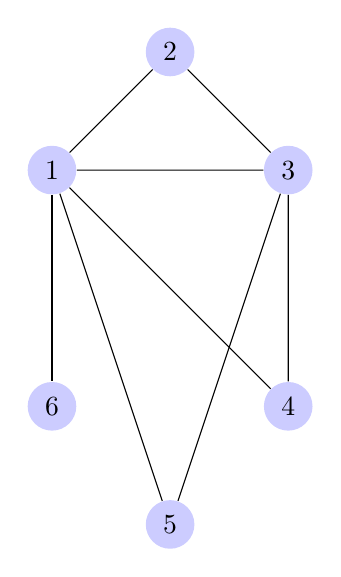
\begin{tikzpicture}[scale=1.5, every node/.style={circle, fill=blue!20}]
            \node (1) at (0, 2) {1};
            \node (2) at (1, 3) {2};
            \node (3) at (2, 2) {3};
            \node (4) at (2, 0) {4};
            \node (5) at (1, -1) {5};
            \node (6) at (0, 0) {6};
    
            \draw (1) -- (2);
            \draw (1) -- (3);
            \draw (1) -- (4);
            \draw (1) -- (5);
            \draw (1) -- (6);
    
            \draw (2) -- (3);
    
            \draw (3) -- (4);
            \draw (3) -- (5);
        \end{tikzpicture}
    \end{center}


    \item Classical AMG is based on the observation that the \textbf{algebraic smooth error varies slowly in the direction of the matrix's relatively large (negative) coefficients}. This gives us an algebraic way to track smooth errors. However, we still need to define large.

    \begin{definitionbox}[: strong connection]
        Given a threshold $\theta \in \left(0, 1\right)$ we say that $i$ is \textbf{strongly connected} with $j$ if:
        \begin{equation}
            -a_{i,j} \ge \theta \underset{k \ne i}{\max}\left(-a_{i,k}\right)
        \end{equation}
        Let us denote by $S_{i}$ the set of vertices that $i$ is strongly connected to by:
        \begin{equation}
            S_{i} = \left\{j \in N_{i} \: : \: i \text{ strongly connects to } j\right\}
        \end{equation}
        Where:
        \begin{equation*}
            N_{i} = \left\{j \ne i \: : \: a_{i,j} \ne 0\right\}
        \end{equation*}
    \end{definitionbox}
    
    \noindent
    This gives us a strength matrix $S$, with $S_{i}$ as its $i$-th row. AMG uses the concept of \emph{strong connection} to \textbf{decide how strongly nodes (grid points) are connected}. This is based on the matrix coefficients. Strong connections are those \textbf{where the matrix coefficients are relatively large}, indicating significant interactions between grid points.


    \item \textbf{\underline{Standard Coarsening}}. Standard coarsening in AMG involves \textbf{reducing the number of variables} (or degrees of freedom) \textbf{in the problem}. This is achieved by \textbf{selecting a subset of nodes}, known as coarse nodes (\textbf{C-vertices}), while the \textbf{remaining nodes become} fine nodes (\textbf{F-vertices}). The \textbf{goal is to simplify the problem while preserving its essential characteristics}.
    
    \begin{itemize}
    	\item \textbf{C-vertices} (Coarse nodes): These are the selected nodes that will form the coarse grid.
    	
    	\item \textbf{F-vertices} (Fine nodes): These are the remaining nodes that are not selected as coarse nodes.
    \end{itemize}
    To put it simply, in AMG we deal with the original problem on a \emph{fine grid}. However, solving large problems directly on this fine grid can be computationally expensive. To simplify, we \textbf{create several \dquotes{coarser} versions of this grid}, in which the \textbf{problem size is progressively reduced}. This process is called \emph{standard coarsening}.
    
    \begin{flushleft}
    	\textcolor{Green3}{\faIcon{question-circle} \textbf{How can we apply the Standard Coarsening?}}
    \end{flushleft}
    \textbf{\underline{It requires an observation before use}}. The oscillatory error should not be a problem, as this error is typically easier to reduce using standard relaxation methods on fine grids. However, the real dilemma is the smooth error, which can't be reduced by simple relaxation methods. \textbf{When applying standard coarsening, we need to focus on reducing smooth error while building each coarse grid group and preserving the most fundamental information}.
    
    \textbf{\underline{Implementation}}. To achieve this, we need to approach the problem from an algebraic point of view. The smooth error tends to vary slowly along strong connections (edges in the graph). Essentially, strong connections represent significant interactions or relationships between nodes (vertices). By \textbf{coarsening in the direction of} these \textbf{strong connections}, we \textbf{preserve the most critical aspects of the problem}, resulting in a more accurate and efficient MG method. In other words, we focus our coarsening efforts on the most \dquotes{meaningful} parts of the graph, where the important information is.
    
    \textbf{\underline{What happens in practice}}. In practice, standard coarsening \textbf{divides the vertices into} Coarse (\textbf{C-vertices}) and Fine (\textbf{F-vertices that are strongly connected to the C-vertices}) sets. The main idea is to \textbf{ensure that each F-vertex has a strong connection to at least one C-vertex}. This allows us to approximate the values at the F-vertices by a linear combination of the values at the C-vertices, preserving the important relationships in the original problem.
    
    \textbf{\underline{What happens after Standard Coarsening}}. The values at the F-vertices can be expressed as a weighted combination of the values at their neighboring C-vertices. This ensures that the coarser problem is a good approximation of the finer problem.
    
    \newpage
    
    \begin{flushleft}
    	\textcolor{Green3}{\faIcon{tools} \textbf{General Coarsening Algorithm}}
    \end{flushleft}
    Given a strength matrix $S$ indicating the strong connections between nodes, the algorithm is:
    \begin{enumerate}
    	\item \textbf{\underline{Initialization}}. We create an empty set $C$ for Coarse vertices and an empty set $F$ for Fine vertices.
    	
    	\item \textbf{\underline{Select an independent set of C-vertices}}. Choose an independent set of C-vertices from the graph of $S$. An independent set means that no two selected C-vertices are directly connected by a strong connection.
    	
    	The selection process is as follows:
    	\begin{enumerate}
    		\item \textbf{\underline{Choose a C-vertex}}. Start with a node and mark it as a C-vertex. In general, we start at the node with the highest number of strong connections (or highest weight, if applicable).
    		\item \textbf{\underline{Populate Fine vertices set}}. All vertices strongly connected to the previously selected C-vertex become F-vertices.
    		\item \textbf{\underline{Repeat}}. We repeat the process by selecting another vertex from the undecided vertices as a C-vertex and making the vertices strongly connected to it as F-vertices.
    		\item \textbf{\underline{Stop when all vertices are classified as either C-vertex}}\break \textbf{\underline{or F-vertex}}.
    	\end{enumerate}
    	
    	\item \textbf{\underline{Select additional C-vertices}}. Ensure that every F-vertex has a strong connection to at least one C-vertex. If any F-vertex is not strongly connected to a C-vertex, convert that F-vertex into a C-vertex to ensure the interpolation requirements are satisfied.
    \end{enumerate}
\end{enumerate}

\begin{flushleft}
	\textcolor{Red2}{\faIcon{bookmark} \textbf{Interpolation}}
\end{flushleft}
Interpolation is used to \textbf{estimate unknown values at fine nodes (F-nodes) using the known values at coarse nodes (C-nodes)}. It’s crucial for maintaining accuracy and efficiency.

Let $\mathbf{e} = \left( e_{1}, e_{2}, \dots, e_{i}, \dots \right)$ be the error; a simple characterization of algebraic smooth error is $A\mathbf{e} \approx 0$. In other words:
\begin{equation}
	a_{i,i} e_{i} + \displaystyle\sum_{j \in N_{i}} a_{i,j}e_{j} \approx 0 \hspace{2em} i \in F
\end{equation}
The idea is that we want to choose proper weight $w_{i,j}$ such that for any algebraic smooth errors:
\begin{equation*}
	e_{i} \approx \displaystyle\sum_{j \in C} w_{i,j}e_{j} \hspace{2em} i \in F
\end{equation*}
But if we define for $i \in F$:
\begin{itemize}
	\item $C_{i}$ the C-points strongly connected to $i$:
	\begin{equation*}
		C_{i} = C \cap N_{i}
	\end{equation*}
	
	\item $F_{i}^{S}$ the F-points strongly connected to $i$:
	\begin{equation*}
		F_{i} = F \cap N_{i}
	\end{equation*}
	
	\item $C_{i}^{S} = C \cap S_{i}$
	
	\item $N_{i}^{W}$ all points weakly connected to $i$:
	\begin{equation*}
		N_{i}^{W} = \dfrac{N_{i}}{\left(C_{i}^{S} \cup F_{i}^{S}\right)}
	\end{equation*}
\end{itemize}
We can rewrite the characterization of algebraic smooth error as:
\begin{equation}
	a_{i,i} e_{i} + \displaystyle\sum_{j \in N_{i}} a_{i,j}e_{j} = 0 \hspace{2em} \alpha = \dfrac{
		\displaystyle\sum_{j \in N_{i}} a_{i,j}
	}{
		\displaystyle\sum_{j \in C_{i}^{S}} a_{i,j}
	}
\end{equation}
We conclude that the \textbf{formula of direct interpolation} is:
\begin{equation}
	w_{i,j} = \alpha\dfrac{a_{i,j}}{a_{i,i}} \hspace{2em} i \in F, \: j \in C_{i}^{S} \hspace{2em} \alpha = \dfrac{
		\displaystyle\sum_{j \in N_{i}} a_{i,j}
	}{
		\displaystyle\sum_{j \in C_{i}^{S}} a_{i,j}
	}
\end{equation}
The above direct interpolation can be applied as long as $C_{i}^{S}$.

\highspace
\begin{flushleft}
	\textcolor{Red2}{\faIcon{dollar-sign} \textbf{How much does it cost?}}
\end{flushleft}
The cost of each iteration in the Algebraic Multigrid (AMG) method primarily \textbf{depends on the operations involved}, such as smoothing, restriction, interpolation, and correction (the all tools that we have already discussed in the previous pages!). The cost is \textbf{generally linearly proportional to the problem size}. This means that as the problem size increases, the cost increases linearly, making AMG methods efficient for large-scale problems.

\highspace
However, leaving aside the iteration cost for the moment, the \textbf{AMG method is the best of the multigrid methods because the construction of the MG hierarchy is done using only information from the matrix and not from the geometry of the problem}. This is the main and most important key. This is one of the most important reasons to choose AMG, especially in real practice problems.

\highspace
\begin{flushleft}
	\textcolor{Green3}{\faIcon{network-wired} \textbf{Can it be parallelized?}}
\end{flushleft}
AMG is not only the best because it is geometric independent, but also because it lends itself very well to parallelization! In general, \textbf{AMG methods are well suited for parallelization, especially for large problems}. The multi-level structure of AMG allows the workload to be distributed across multiple processors. However, the efficiency of parallelization depends on the specific implementation and the problem to be solved (of course). Optimizations and careful communication management can help achieve better parallel performance.


    %%%%%%%%%%%%%%%%%%%%%%%%%%%%%%%%
    % Domain Decomposition Methods %
    %%%%%%%%%%%%%%%%%%%%%%%%%%%%%%%%
    \section{CUDA}

\subsection{Introduction}

\definition{CUDA}, which stands for \textbf{Compute Unified Device Architecture}, is a \textbf{parallel computing platform and application programming interface (API) model created by NVIDIA}. It allows developers to use the power of GPUs (Graphics Processing Units) for general-purpose processing, which enables substantial performance improvements for computationally intensive tasks.

\highspace
\begin{flushleft}
    \textcolor{Green3}{\faIcon{question-circle} \textbf{Why CUDA?}}
\end{flushleft}
GPUs, originally designed to render graphics, have evolved into \textbf{highly efficient and powerful processors capable of handling thousands of threads simultaneously}. This transformation has made GPUs, and by extension CUDA, incredibly valuable for applications requiring massive parallelism, such as scientific simulations, machine learning, and deep learning.

\highspace
\begin{flushleft}
    \textcolor{Green3}{\faIcon{question-circle} \textbf{Why can we not just use the CPU?}}
\end{flushleft}
Understanding the fundamental differences between CPU and GPU architectures is key to appreciating CUDA's advantages:
\begin{itemize}
    \item CPU (Central Processing Unit):
    \begin{itemize}
        \item Designed for sequential processing.
        \item Features powerful Arithmetic Logic Units (ALUs) with low latency.
        \item Utilizes large hierarchical caches to optimize access to frequently used data.
        \item Employs advanced control mechanisms, such as branch prediction and data forwarding, to minimize delays.
    \end{itemize}

    \item GPU (Graphics Processing Unit):
    \begin{itemize}
        \item Optimized for parallel processing.
        \item Contains a large number of simpler, pipelined ALUs designed for high-throughput computations, despite having longer latency.
        \item Relies on smaller caches to facilitate high memory throughput.
        \item Uses simpler control mechanisms, enabling efficient context switching and handling many threads concurrently.
    \end{itemize}
\end{itemize}
CUDA leverages these GPU characteristics to execute programs with a parallel-first approach, breaking down tasks into smaller, manageable pieces and processing them simultaneously. This approach leads to significant speedups compared to traditional CPU-only processing, making CUDA a pivotal technology for high-performance computing.

    \subsection{Overlapping Subdomains}

\definition{Overlapping Subdomains} refer to the concept within Domain Decomposition Methods where the \textbf{computational domain is divided into smaller regions that share some common boundaries}. These shared boundaries are what make them \emph{overlapping}. This method is widely used to \textbf{enhance the convergence and accuracy of solving large-scale computational problems}, particularly partial differential equations (PDEs).

\highspace
\begin{flushleft}
    \textcolor{Green3}{\faIcon{tools} \textbf{Key Characteristics of Overlapping Subdomains}}
\end{flushleft}
\begin{enumerate}
    \item \textbf{Shared Boundaries}: The subdomains have regions where their boundaries overlap with adjacent subdomains. This overlapping region is critical for the exchange of information between subdomains.
    \item \textbf{Independent Solutions}: Each subdomain is solved independently, often in parallel, using updated boundary conditions from adjacent subdomains.
    \item \textbf{Iterative Process}: Solutions are updated iteratively by alternating between solving the subdomains and using the latest boundary conditions. This process continues until convergence is achieved.
\end{enumerate}

\begin{examplebox}
    Suppose we have a domain $\Omega$ that we want to solve a PDE on. We can divide $\Omega$ into two overlapping subdomains $\Omega_{1}$ and $\Omega_{2}$:
    \begin{itemize}
        \item Subdomain $\Omega_{1}$: Contains a portion of $\Omega$ and overlaps with $\Omega_{2}$ at the boundary.
        \item Subdomain $\Omega_{2}$: Contains another portion of $\Omega$ and overlaps with $\Omega_{1}$ at the boundary.
    \end{itemize}
\end{examplebox}

\highspace
\begin{flushleft}
    \textcolor{Green3}{\faIcon{check-circle} \textbf{Benefits of Overlapping Subdomains}}
\end{flushleft}
\begin{enumerate}
    \item \textbf{Improved Boundary Condition Handling}: The overlapping regions allow for better and more accurate boundary condition updates, leading to improved convergence rates.
    \item \textbf{Enhanced Convergence}: The iterative updates and information exchange in the overlapping regions help accelerate the convergence of the solution.
    \item \textbf{Parallel Processing}: Each subdomain can be solved independently, making it suitable for parallel computing, which significantly reduces computation time.
\end{enumerate}

\newpage

\subsubsection{Alternating Schwarz Method}

The \definition{Alternating Schwarz Method} is a classical \textbf{iterative technique} used in numerical linear algebra \textbf{to solve partial differential equations (PDEs)}. It is a type of domain decomposition method that divides the computational domain into overlapping subdomains.

\highspace
\begin{flushleft}
    \textcolor{Green3}{\faIcon{lightbulb} \textbf{Main idea}}
\end{flushleft}
\begin{itemize}
    \item \important{Domain Decomposition}: The main idea is to \textbf{break down a large problem into smaller, overlapping subproblems}. By solving these smaller problems iteratively, the overall solution can be efficiently approximated.
    \item \important{Overlap}: \textbf{Subdomains overlap at their boundaries}, allowing for more accurate boundary condition updates and improving the convergence rate of the method.
\end{itemize}

\highspace
\begin{flushleft}
    \textcolor{Green3}{\faIcon{tools} \textbf{Algorithm}}
\end{flushleft}
\begin{enumerate}
    \item \textbf{Initialization}: Start with an \emph{initial guess} for the solution over the entire domain.
    \item \textbf{Subdomain Solutions}: Alternately solve the PDE on each subdomain:
    \begin{itemize}
        \item On the first subdomain, using boundary conditions updated from the initial guess or the latest solution.
        \item On the second subdomain, using boundary conditions updated from the solution of the first subdomain.
    \end{itemize}
    \item \textbf{Iteration}: Continue alternating between subdomains, \textbf{updating the solution iteratively until convergence is achieved}.
\end{enumerate}

\highspace
\begin{examplebox}[: Elliptic Partial Differential Equation (PDE)]
    The problem involves solving an elliptic PDE of the form:
    \begin{equation*}
        Lu = f \hspace{1em} \text{in} \; \Omega = \Omega_{1} \cup \Omega_{2}
    \end{equation*}
    Where:
    \begin{itemize}
        \item $L$ is the \textbf{differential operator}.
        \item $u$ is the \textbf{unknown function we are solving for}.
        \item $f$ is a given function representing \textbf{the source term}.
        \item $\Omega$ is the \textbf{computational domain}, divided into two overlapping subdomains $\Omega_{1}$ and $\Omega_{2}$.
    \end{itemize}
    The boundary condition is:
    \begin{equation*}
        u = g \hspace{1em} \text{on} \; \partial \Omega
    \end{equation*}
    Here, $\partial \Omega$ represents the \textbf{boundary of the entire domain}.

    \highspace
    \textbf{Domain Decomposition}. The domain $\Omega$ is divided into two overlapping subdomains $\Omega_{1}$ and $\Omega_{2}$, each with its own boundary:
    \begin{itemize}
        \item $\Gamma_{1}$ is the boundary of $\Omega_{1}$.
        \item $\Gamma_{2}$ is the boundary of $\Omega_{2}$.
    \end{itemize}
    These subdomains overlap at certain regions, allowing for the exchange of boundary conditions and improving the overall convergence.
    \begin{center}
        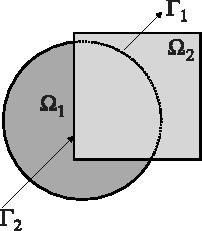
\includegraphics[width=.3\textwidth]{img/elliptic-pde-1.pdf}
    \end{center}

    \highspace
    \textbf{Iterative Solution Process}. The Alternating Schwarz Method iteratively solves the PDE on each subdomain while updating the boundary conditions based on the solutions from neighboring subdomains. The process involves the following steps:
    \begin{enumerate}
        \item \textbf{Initialization}. Start with an initial guess $ u^{(0)} $ for the solution.
        
        \item \textbf{Subdomain Solutions}:
        \begin{itemize}
            \item On $\Omega_{1}$:
            \begin{equation*}
                \begin{cases}
                    L u_{1}^{\left(k+\frac{1}{2}\right)} = f & \text{in} \; \Omega_{1} \vspace{.5em}\\
                    u_{1}^{\left(k+\frac{1}{2}\right)} = g & \text{on} \; \partial \Omega_{1} \setminus \Gamma_{1} \vspace{.5em}\\
                    u_{1}^{\left(k+\frac{1}{2}\right)} = u_{2}^{(k)} & \text{on} \; \Gamma_{1}
                \end{cases}
            \end{equation*}

            \item On $\Omega_{2}$:
            \begin{equation*}
                \begin{cases}
                    L u_{2}^{(k+1)} = f & \text{in} \; \Omega_{2} \vspace{.5em}\\
                    u_{2}^{(k+1)} = g & \text{on} \; \partial \Omega_{2} \setminus \Gamma_{2} \vspace{.5em}\\
                    u_{2}^{(k+1)} = u_{1}^{(k+\frac{1}{2})} & \text{on} \; \Gamma_{2}
                \end{cases}
            \end{equation*}
        \end{itemize}

        \item \textbf{Update}. Combine solutions to form the updated solution $u^{\left(k+1\right)}$:
        \begin{equation*}
            u^{(k+1)} =
            \begin{cases}
                u_{1}^{\left(k+\frac{1}{2}\right)} & \text{in} \; \Omega_{1} \setminus \Omega_{2} \vspace{.5em}\\
                u_{2}^{\left(k+1\right)} & \text{in} \; \Omega_{2}
            \end{cases}
        \end{equation*}
    \end{enumerate}

    \highspace
    \textbf{Convergence}. The iterative \textbf{process continues until the solutions on the overlapping subdomains converge to a stable solution for the entire domain} $\Omega$. The convergence rate is often enhanced due to the overlap and the iterative updating of boundary conditions.
\end{examplebox}
    \subsubsection{Discretized Schwarz Methods}

The \definition{Discretized Schwarz Methods} involve \textbf{applying the Schwarz decomposition principles to a discretized version of the computational domain}. This results in an algebraic system that can be efficiently solved using the same iterative techniques.

\begin{itemize}
    \item \important{Discretization Process}. The \textbf{continuous domain is discretized into a grid or mesh}, resulting in a \textbf{finite set of points that represent the domain}. The PDE is then transformed into a system of linear equations:
    \begin{equation*}
        A\mathbf{x} = \mathbf{b}
    \end{equation*}
    \begin{itemize}
        \item $A$ matrix representing the \emph{discretized operator};
        \item $\mathbf{x}$ is the \emph{vector of unknowns};
        \item $\mathbf{b}$ represents the \emph{source terms} or \emph{boundary conditions}.
    \end{itemize}


    \item \important{Overlapping Subdomains}: Each subdomain $\Omega_{i}$ has a \textbf{set of grid points} ($n$) indexed by $S_{i}$ (with $n_{i} = \left|S_{i}\right|$). The \textbf{overlap between subdomains ensures that the indices in} $ S_1 $ and $ S_2 $ are \textbf{not disjoint} ($S_{1} \cap S_{2} \ne \emptyset$ and $n_{1} + n_{2} > n$), facilitating the exchange of boundary information.


    \item \important{Boolean Restriction Matrices}: Boolean restriction matrices $ R_{i}$ are used to \textbf{extract the relevant components of the solution vector} $\mathbf{v}$ \textbf{for each subdomain}. These matrices play a crucial role in the iterative solution process by ensuring that each subdomain only processes its relevant data.

    Formally, for $i = 1, 2$, let $R_{i}$ be an $n_{i} \times n$ boolean restriction matrix such that for any vector $\mathbf{v} \in \mathbb{R}^{n}$:
    \begin{equation*}
        \mathbf{v}_{i} = R_{i} \mathbf{v} \in \mathbb{R}^{n_{i}}
    \end{equation*}
    This means $\mathbf{v}_{i}$ contains the components of $\mathbf{v}$ corresponding to indices in $ S_{i}$ (i.e., those components associated with nodes in $\Omega_{i}$).


    \item \important{Extension Matrices}: Extension matrices are used to \textbf{expand the solution from subdomains back to the global domain}. The extension matrix $R_{i}^{T}$ maps the local solution $\mathbf{v}_{i}$ back to the global solution $\mathbf{v}$.

    Formally, for $i = 1, 2$:
    \begin{equation*}
        \mathbf{v} = R_{i}^{T} \mathbf{v}_{i}
    \end{equation*}
    This ensures that the components of $\mathbf{v}$ corresponding to indices in $S_{i}$ are the same as those of $\mathbf{v}_{i}$, while the remaining components are zero.


    \item \important{Principal Submatrices}: Principal submatrices are \textbf{submatrices} of the global matrix $\mathbf{A}$ \textbf{that correspond to the subdomains}. For each subdomain $\Omega_{i}$, the principal submatrix $\mathbf{A}_{i}$ is formed by restricting $\mathbf{A}$ to the indices in $S_{i}$.

    Formally, for subdomain $\Omega_{i}$, the principal submatrix $A_{i} \in \mathbb{R}^{n_{i} \times n_{i}}$ is given by:
    \begin{equation}\label{eq: principal submatrices - discretized schwarz methods}
        \mathbf{A}_{i} = R_{i} \mathbf{A} R_{i}^{T}
    \end{equation}
    These submatrices represent the \textbf{system of equations for the respective subdomains}, allowing them to be solved independently.
\end{itemize}

\begin{flushleft}
    \textcolor{Green3}{\faIcon{book} \textbf{Linking the Concepts}}
\end{flushleft}
\begin{itemize}
    \item \important{Extension Matrices and Boolean Restriction Matrices}. The extension matrices $R_i^T$ and the boolean restriction matrices $R_i$ are \textbf{complementary}.
    \begin{itemize}
    	\item Extension Matrices $R_{i}$ \textbf{extracts} the relevant \textbf{components of the solution} vector $\mathbf{v}$ \textbf{for each subdomain};
    	\item Boolean Restriction Matrices $R_{i}^{T}$ \textbf{extends} the \textbf{local solution} $\mathbf{v}_{i}$ \textbf{back to the global solution} $\mathbf{v}$.
    \end{itemize}

    \item \important{Principal Submatrices and Overlapping Subdomains}. The principal submatrices $\mathbf{A}_{i}$ are directly related to the overlapping subdomains. \textbf{Each subdomain $\Omega_{i}$ has its own principal submatrix $\mathbf{A}_{i}$, which represents the local system of equations}. The overlap between subdomains ensures that the principal submatrices share common indices, facilitating the exchange of boundary information and ensuring consistency in the global solution.
\end{itemize}

\highspace
The following pages introduce two types of Discretized Schwarz methods:
\begin{enumerate}
    \item \textbf{Multiplicative Schwarz method}, where subdomains are updated sequentially. The solution from each subdomain is used to update the boundary conditions for the next subdomain in the sequence.

    \item \textbf{Additive Schwarz method}, where subdomains are solved independently and their solutions are combined additively to form the global solution.
\end{enumerate}
    \paragraph{Multiplicative Schwarz method}

The \definition{Multiplicative Schwarz Method} is an \textbf{iterative technique used to solve discretized linear systems}, particularly in the context of domain decomposition methods. It is similar to the block Gauss-Seidel method but uses overlapping blocks. The method involves breaking down a large system into smaller subproblems that can be solved more easily.

\begin{enumerate}
    \item \textbf{Principal Submatrices}. The matrix $A$ is decomposed into principal submatrices $A_{1}$ and $A_{2}$, corresponding to two subdomains. These submatrices are given by (with eq. \ref{eq: principal submatrices - discretized schwarz methods}, page \pageref{eq: principal submatrices - discretized schwarz methods}):
    \begin{equation*}
        \begin{array}{rcl}
            A_{1} &=& R_{1} A R_{1}^{T} \\ [.5em]
            A_{2} &=& R_{2} A R_{2}^{T}
        \end{array}
    \end{equation*}
    Where $R_{1}$ and $R_{2}$ are restriction operators that extract the relevant components for each subdomain.

    \item \textbf{Alternating Schwarz Iteration}. For a discretized problem, the alternating Schwarz iteration takes the following form:
    \begin{equation*}
        \begin{array}{rcl}
            x^{\left(k+\frac{1}{2}\right)} &=& x^{(k)} + R_{1}^{T} A_{1}^{-1} R_{1} \left(b - A x^{(k)}\right) \\ [.5em]
            x^{(k+1)} &=& x^{\left(k+\frac{1}{2}\right)} + R_{2}^{T} A_{2}^{-1} R_{2} \left(b - A x^{\left(k+\frac{1}{2}\right)}\right)
        \end{array}
    \end{equation*}
    These equations update the solution vector $x$ by solving the subproblems within each subdomain iteratively.

    \item \textbf{Error Update}. The overall error $e^{(k)} = x - x^{(k)}$ is updated as:
    \begin{equation*}
        e^{(k+1)} = B_{MS} e^{(k)}
    \end{equation*}
    Where:
    \begin{equation*}
        B_{MS} = \left(I - R_{2}^{T} A_{2}^{-1} R_{2} A\right)\left(I - R_{1}^{T} A_{1}^{-1} R_{1} A\right)
    \end{equation*}
    The \textbf{error propagation matrix} $B_{MS}$ shows how the \textbf{error evolves through each iteration}, ensuring convergence of the method.
\end{enumerate}

\highspace
\begin{flushleft}
    \textcolor{Green3}{\faIcon{book} \textbf{Sequential Nature of the Multiplicative Schwarz Method}}
\end{flushleft}
The Multiplicative Schwarz Method involves \textbf{sequential computation}, which can be both a strength and a limitation depending on the context of its application. 
\begin{itemize}
    \item \important{Subdomain Dependency}. In the Multiplicative Schwarz Method, \textbf{each subdomain's solution depends on the updated solution of the previous subdomain}. This dependency requires that subdomains be solved in a specific sequence. For example, subdomain $\Omega_{2}$ uses the updated boundary conditions from the solution of subdomain $\Omega_{1}$.


    \item \important{Iteration Steps}. The method alternates between solving subdomain problems, updating the boundary conditions iteratively. Here's the typical update process:
    \begin{equation*}
        \begin{array}{rcl}
            \mathbf{x}^{\left(k+\frac{1}{2}\right)} &=& \mathbf{x}^{(k)} + R_{1}^{T} A_{1}^{-1} R_{1} \left(\mathbf{b} - A \mathbf{x}^{(k)}\right) \\ [.7em]
            \mathbf{x}^{(k+1)} &=& \textcolor{Red2}{\mathbf{x}^{\left(k+\frac{1}{2}\right)}} + R_{2}^{T} A_{2}^{-1} R_{2} \left(\mathbf{b} - A \textcolor{Red2}{\mathbf{x}^{\left(k+\frac{1}{2}\right)}}\right)
        \end{array}
    \end{equation*}
    Subdomain $\Omega_{2}$ cannot be updated until subdomain $\Omega_{1}$ has been solved and its results incorporated.
\end{itemize}
In fact, the method is called \emph{multiplicative} because:
\begin{enumerate}
    \item Each subdomain solution depends on the updated boundary conditions from the previous subdomain, effectively \emph{multiplying} the effect of each update;
    \item The error update formula for the Multiplicative Schwarz Method involves the sequential multiplication of error reduction operators for each subdomain.
\end{enumerate}
However, there are limitations:
\begin{itemize}
    \item \important{Lack of Parallelism}. Because of the sequential nature, \textbf{subdomains must be processed one after the other}, making it difficult to exploit parallel computing resources effectively. This limits the scalability of the method on modern high-performance computing systems, where parallelism is crucial for handling large-scale problems efficiently.

    \item \important{Longer Computation Times}. Sequential updates mean that each iteration can take longer compared to methods that allow for parallel processing. The overall computation time increases, especially for problems with many subdomains or very large domains.

    \item \important{Communication Overhead}. In distributed computing environments, the sequential nature can result in increased communication overhead between processors, as each processor must wait for the previous one to complete its computation before starting.
\end{itemize}

\highspace
\begin{flushleft}
    \textcolor{Green3}{\faIcon{book} \textbf{Gauss-Seidel Analogy}}
\end{flushleft}
The Multiplicative Schwarz Method is analogous to the block Gauss-Seidel method. Just like the Gauss-Seidel method updates the solution iteratively using previously computed values, the Multiplicative Schwarz Method updates the solution sequentially by \emph{multiplying} the effect of each subdomain's solution.

\highspace
\begin{flushleft}
    \textcolor{Green3}{\faIcon{check-circle} \textbf{Pros}}
\end{flushleft}
Can lead to \textbf{faster convergence for certain problems} due to the sequential dependency of updates.

\highspace
\begin{flushleft}
    \textcolor{Red2}{\faIcon{times-circle} \textbf{Cons}}
\end{flushleft}
Limited by its sequential nature, making it \textbf{less suitable for parallel processing}.
    \paragraph{Additive Schwarz method}

The \definition{Additive Schwarz method} is a \textbf{domain decomposition method that allows subproblems to be solved in parallel}, unlike the Multiplicative Schwarz Method. This method is particularly suitable for parallel computing environments, making it \textbf{highly efficient for large-scale problems}.

\highspace
\begin{flushleft}
    \textcolor{Green3}{\faIcon{tools} \textbf{Main features}}
\end{flushleft}
\begin{itemize}
    \item[\textcolor{Green3}{\faIcon{check}}] \textcolor{Green3}{\textbf{Parallelism}}. The Additive Schwarz Method achieves \textbf{parallelism by solving subproblems simultaneously}. This is in contrast to the sequential approach of the Multiplicative Schwarz Method, where subproblems are solved one after another.

    \item \important{Block Jacobi Approach}. The method uses a \textbf{block Jacobi approach} instead of a block Gauss-Seidel approach. In the block Jacobi approach, \textbf{each subdomain problem is solved independently}, allowing for parallel execution.
    
    \item \important{Equations and Iteration Steps}. The iterative process involves updating the solution vector $\mathbf{x}$ by combining the solutions from all subdomains additively:
    \begin{equation*}
        \begin{array}{rcl}
            \mathbf{x}^{\left(k+\frac{1}{2}\right)} &=& \mathbf{x}^{(k)} + R_{1}^{T} A_{1}^{-1} R_{1} \left(\mathbf{b} - A \mathbf{x}^{(k)}\right) \\ [.7em]
            \mathbf{x}^{(k+1)} &=& \mathbf{x}^{\left(k+\frac{1}{2}\right)} + \underbrace{R_{2}^{T} A_{2}^{-1} R_{2} \left(\mathbf{b} - A \mathbf{x}^{(k)}\right)}_{\text{independently of }\mathbf{x}^{\left(k+\frac{1}{2}\right)}}
        \end{array}
    \end{equation*}
    These equations indicate that the solutions for subdomains $\Omega_{1}$ and $\Omega_{2}$ can be \textbf{computed simultaneously}.

    \item \important{Error Update}. The overall error $\mathbf{e}^{(k)} = \mathbf{x} - \mathbf{x}^{(k)}$ is updated as:
    \begin{equation*}
        \mathbf{e}^{(k+1)} = B_{AS} \mathbf{e}^{(k)}
    \end{equation*}
    where:
    \begin{equation*}
        B_{AS} = (R_{2}^{T} A_{2}^{-1} R_{2} + R_{1}^{T} A_{1}^{-1} R_{1}) A
    \end{equation*}
    The error propagation matrix $B_{AS}$ reflects the additive nature of the method, combining the effects of all subdomain solutions.
\end{itemize}

\newpage

\begin{flushleft}
    \textcolor{Green3}{\faIcon{tachometer-alt} \textbf{Additive Schwarz Preconditioner}}
\end{flushleft}
The two separate equations for the Additive Schwarz Method can be \textbf{combined into a single update equation by introducing an} \definition{Additive Schwarz Preconditioner}. This preconditioner combines the effects of all subdomain solutions into one equation, simplifying the iterative process. The combined update equation is:
\begin{equation}
    x^{\left(k+1\right)} = x^{\left(k\right)} + P_{ad}^{-1}\mathbf{r}^{\left(k\right)} \hspace{2em} k \ge 0
\end{equation}
where $P_{ad}^{-1}$ is the additive Schwarz preconditioner:
\begin{equation}
    P_{ad}^{-1} = \left(
        R_{1}^{T}A_{1}^{-1}R_{1} +
        R_{2}^{T}A_{2}^{-1}R_{2}
    \right)
\end{equation}
\begin{proof}
    To simplify the formulation, we can eliminate the intermediate step $x^{\left(k+\frac{1}{2}\right)}$ to obtain a direct update equation:
    \begin{equation*}
        x^{\left(k+1\right)} = x^{\left(k\right)} + R_{1}^{T}A_{1}^{-1}R_{1}\left(\mathbf{b} - A\mathbf{x}^{\left(k\right)}\right) + R_{2}^{T}A_{2}^{-1}R_{2}\left(\mathbf{b} - A\mathbf{x}^{\left(k\right)}\right)
    \end{equation*}
    This simplifies to:
    \begin{equation*}
        \begin{array}{rcl}
            x^{\left(k+1\right)} &=& x^{\left(k\right)} + \left(
                R_{1}^{T}A_{1}^{-1}R_{1} + R_{2}^{T}A_{2}^{-1}R_{2}
            \right) \left(\mathbf{b} - A\mathbf{x}^{\left(k\right)}\right) \\ [.7em]
            &=& x^{\left(k\right)} + \left(
                R_{1}^{T}A_{1}^{-1}R_{1} + R_{2}^{T}A_{2}^{-1}R_{2}
            \right) \left(\mathbf{r}^{\left(k\right)}\right)
        \end{array}
    \end{equation*}
    Where:
    \begin{itemize}
        \item $\mathbf{r}^{\left(k\right)}$ is the residual vector $\mathbf{b} - A\mathbf{x}^{\left(k\right)}$;
        \item $\left(R_{1}^{T}A_{1}^{-1}R_{1} + R_{2}^{T}A_{2}^{-1}R_{2}\right)$ is the preconditioner $P_{ad}^{-1}$.
    \end{itemize}
\end{proof}

\noindent
The additive Schwarz preconditioner is \textbf{used to improve the convergence rate} of the iterative solver by combining the effects of all subdomain solutions.

\highspace
\begin{flushleft}
    \textcolor{Green3}{\faIcon{book} \textbf{Symmetry of Preconditioner (and PCG)}}
\end{flushleft}
The preconditioner $P_{ad}^{-1}$ retains the \textbf{symmetry} of the original matrix $A$. This is important because it \textbf{ensures compatibility with the Preconditioned Conjugate Gradient (PCG) method}, which requires the system to be symmetric and positive-definite. It is an iterative solver for symmetric positive-definite linear systems. However, the equation for \textbf{PCG with the additive Schwarz preconditioner} is:
\begin{equation}
    \mathbf{x}^{\left(k+1\right)} = \mathbf{x}^{\left(k\right)} + \alpha_{k}P^{-1}_{ad}\mathbf{p}^{\left(k\right)} \hspace{2em} k \ge 0
\end{equation}
Here, $\alpha_{k}$ is a step size, and $\mathbf{p}^{\left(k\right)}$ is the search direction at iteration $k$ (see chapter \ref{subsection: Conjugate Gradient method}, on page \pageref{subsection: Conjugate Gradient method}, for a refresher on Conjugate Gradient).

\newpage

\begin{flushleft}
    \textcolor{Green3}{\faIcon{star} \textbf{Symmetrized Multiplicative Schwarz Preconditioner}}
\end{flushleft}
The \textbf{standard multiplicative Schwarz iteration matrix is not symmetric}, which can be a limitation when using methods like PCG that require symmetry. To address this, an additional step involving $A_{1}^{-1}$ is introduced to make the preconditioner symmetric:
\begin{enumerate}
    \item First Symmetric Step:
    \begin{equation}
        \mathbf{x}^{\left(k+\frac{1}{3}\right)} = \mathbf{x}^{\left(k\right)} + R_{1}^{T}A_{1}^{-1}R_{1}\left(\mathbf{b}-A\mathbf{x}^{\left(k\right)}\right)
    \end{equation}

    \item Second Symmetric Step:
    \begin{equation}
        \mathbf{x}^{\left(k+\frac{2}{3}\right)} = \mathbf{x}^{\left(k+\frac{1}{3}\right)} + R_{2}^{T}A_{2}^{-1}R_{2}\left(\mathbf{b}-A\mathbf{x}^{\left(k+\frac{1}{3}\right)}\right)
    \end{equation}

    \item Third Symmetric Step:
    \begin{equation}
        \mathbf{x}^{\left(k+1\right)} = \mathbf{x}^{\left(k+\frac{2}{3}\right)} + R_{1}^{T}A_{1}^{-1}R_{1}\left(\mathbf{b}-A\mathbf{x}^{\left(k+\frac{2}{3}\right)}\right)
    \end{equation}
\end{enumerate}
This process results in a symmetric preconditioner $P_{mus}^{-1}$ that can be used effectively with the PCG method to accelerate convergence:
\begin{equation}
    \mathbf{x}^{\left(k+1\right)} = \mathbf{x}^{\left(k\right)} + \alpha_{k}P_{mus}^{-1}\mathbf{r}^{\left(k\right)} \hspace{2em} k \ge 0
\end{equation}

    % 1. **Introduction to Domain Decomposition Methods**
    %    - Brief overview of what Domain Decomposition Methods are and their importance
    % 
    % 2. **Overlapping Subdomains**
    %    1. **Alternating Schwarz Method**
    %       - Explanation and examples
    %    2. **Discretized Schwarz Methods**
    %       - How discretization is applied in Schwarz methods
    %    3. **Additive Schwarz Method**
    %       - Detailed explanation and applications
    %    4. **Additive Schwarz Preconditioner**
    %       - How preconditioners improve the efficiency of additive Schwarz methods
    %    5. **Symmetrized Multiplicative Schwarz Preconditioner**
    %       - Explanation and significance of symmetrized preconditioning
    %    6. **Many Overlapping Subdomains**
    %       - Handling multiple overlapping subdomains and their challenges
    %    7. **Colouring Techniques**
    %       - Techniques used for efficient overlapping and decomposition
    % 
    % 3. **Non-Overlapping Subdomains**
    %    1. **Non-Overlapping Subdomains**
    %       - Introduction to non-overlapping methods
    %    2. **The Schur Complement**
    %       - Explanation and applications in non-overlapping methods
    %    3. **Many Non-Overlapping Subdomains**
    %       - Handling multiple non-overlapping subdomains
    % 
    % 4. **Evaluating Efficiency**
    %    - **How to Evaluate the Efficiency of a Domain Decomposition?**
    %      - Metrics and methods for evaluating the performance of domain decomposition methods


    %%%%%%%%%%%%%%%%%%%%%%%%%%
    % Bibliography and index %
    %%%%%%%%%%%%%%%%%%%%%%%%%%
    \pagestyle{fancy}
\fancyhead{} % clear all header fields
\fancyhead[R]{\nouppercase{\leftmark}}

\bibliography{bibtex}{}
\bibliographystyle{plain}

\newpage

\printindex
\end{document}